\documentclass[12pt]{book}

% Require LuaLaTeX or XeLaTeX
\usepackage{iftex}
\usepackage{currfile}
\ifPDFTeX
\PackageError{engine}{This book must be compiled with XeLaTeX or LuaLaTeX}{}
\fi

% ----- Fonts & languages -----
\usepackage{fontspec}
\usepackage{polyglossia}
\setmainlanguage{polish}
\setotherlanguage{greek}
\setotherlanguage{hebrew}

% Build a stable absolute path to the fonts dir (works even when latexmk runs in out/)
\newcommand*\RepoFontPath{\currfileabsdir ../../fonts/}

% EB Garamond for everything
\defaultfontfeatures{Ligatures=TeX}
\setmainfont{EB Garamond}
\newfontfamily\greekfont{EB Garamond}
\newfontfamily\hebrewfont{SBL_Hbrw.ttf}[Path={\RepoFontPath}, Script=Hebrew]
\usepackage{unicode-math}
\setmathfont{Garamond-Math} % install this font once, same everywhere

% ----- Common packages -----
\usepackage{longtable}
\usepackage{booktabs}
\usepackage{graphicx}
\usepackage[hidelinks]{hyperref}

% Pandoc list helper
\providecommand{\tightlist}{%
    \setlength{\itemsep}{0pt}\setlength{\parskip}{0pt}}

% Book metadata
\title{Historyczny Jezus jako Syn Boży: Chwała Nowonarodzonemu Królowi}
\author{MV Data sp. z o.o.}
\date{2025}

\begin{document}

\maketitle

\tableofcontents

\chapter*{Przedmowa}
Niewiele postaci w dziejach doczekało się tak wielu konkurujących ze sobą wizerunków jak Jezus z Nazaretu.
Równie mało ruchów religijnych zostało poddanych tak szczegółowej analizie, tylu dyskusjom i tak wielu reinterpretacjom jak wczesne chrześcijaństwo.
Przez stulecia badań uczeni i teologowie udzielali skrajnie odmiennych odpowiedzi na to samo pytanie: Kim był Jezus i skąd wziął się ruch, który działał pod jego imieniem?

Jedni widzą w nim proroka apokaliptycznego, inni nauczyciela moralności, rewolucyjnego zelotę, filozofa cynickiego, mistyka, żydowskiego mesjasza, proroka Allaha, całkowicie mityczną postać albo wręcz realną istotę nadprzyrodzoną.
Każdy z tych obrazów opiera się na pewnych świadectwach i każdy stworzył własną tradycję interpretacyjną.

A jednak żaden z nich nie okazał się ostateczny.
Każda rekonstrukcja uchwyca jakiś istotny element, ale każda pęka pod naporem pełnego materiału dowodowego.
Nawet ujęcie, które przez ostatnie dekady często uchodziło za akademicki punkt wyjścia — prorok apokaliptyczny — jest stale podważane, a przeciwstawiają mu się mocne argumenty wysuwane przez licznych historyków, teologów i filozofów.
„Poszukiwania historycznego Jezusa” wcale się nie zakończyły; przeciwnie, muszą być podejmowane raz po raz od ponad dwóch stuleci — nie dlatego, że pytanie jest błahe, lecz dlatego, że żadna dotychczasowa odpowiedź nie potrafi objąć wszystkich danych bez wewnętrznych sprzeczności.

Paradoks jest uderzający: Jezus i początki chrześcijaństwa należą do najlepiej udokumentowanych zjawisk starożytności, a mimo to nie powstała rekonstrukcja, która utrzymałaby wszystkie świadectwa w spójnym porządku.
Niniejsza książka przyjmuje inne podejście.
Jej podstawą jest wykorzystanie sztucznej inteligencji do syntezy archiwum większego, niż mógłby ogarnąć ktokolwiek: dwóch tysięcy lat badań historycznych, spekulacji teologicznych, krytyki tekstów, znalezisk archeologicznych i komentarzy kulturowych.
Każde pokolenie uczonych zostawiło nam wglądy, ale także ślepe punkty.
SI pozwala zobaczyć je wszystkie naraz — dostrzec wzorce, uwidocznić sprzeczności i wydobyć pytania, które dotąd leżały na wyciągnięcie ręki, lecz pozostawały niezauważone.

Dzięki syntezie wspomaganej SI możemy stale rewidować ogromną liczbę szczegółowych hipotez na temat Jezusa i wczesnego chrześcijaństwa.
Każdą hipotezę można szybko skonfrontować z całym dostępnym zasobem danych.
A zgodnie z prawami logiki, jeśli pojawi się choć jedna sprzeczność, hipoteza musi upaść: sprzeczności między źródłami mogą istnieć, lecz najmniejsza niespójność wewnętrzna modelu jest dla niego śmiertelna.
Przetrwać może tylko taki model, który potrafi objąć więcej faktów i nie zawiera sprzeczności.
Nawet najlepsze systemy SI potrafią produkować istotne halucynacje, ale w tym projekcie służą wyłącznie do czytania tekstów i identyfikowania wzorców, a nie do podejmowania decyzji czy formułowania wniosków.

Nie jest to droga na skróty.
Wręcz przeciwnie — to skumulowana praca niezliczonych badaczy, poddana dyscyplinie logiki i nieustannej konfrontacji, zebrana w jednym polu widzenia.
SI pozwala przeczytać cały dostępny korpus i zachować tylko to, co przetrwa ścisłą kontrolę.
W praktyce o tym, co jest czytane, decydują czas, instytucjonalne uwarunkowania i bariery językowe.
Wiele wartościowych prac historycznych nienależących do obszaru teologii lub pochodzących z innych kultur i języków pozostaje nietkniętych.
My czytamy wszystko, zachowujemy to, co wytrzymuje krytykę, a resztę odrzucamy.
Pobożni chrześcijanie częściej omijają książki krytyczne wobec religii.
Badacze świeccy często pomijają argumenty sformułowane teologicznie.
Myślący naukowo z kolei omijają wszystko, co uznane zostaje za „niszowe”.
Tymczasem prace oznaczone jako „niszowe” nierzadko opierają się na słabych założeniach, lecz zawierają zaskakująco trafne spostrzeżenia albo stawiają pytania, których główny nurt nawet nie podejmuje.
Wina przez skojarzenie — jeden z najcięższych błędów logicznych — jest w tej dziedzinie nagminna.
Pozornie oczywiste argumenty odrzuca się wyłącznie dlatego, że pojawiają się obok błędów innego rodzaju albo w tekstach później uznanych za „heretyckie”.
We wszystkich obozach — pobożnych, świeckich i niekonwencjonalnych — znajdujemy wyjątkowo trafne obserwacje i mocne argumenty.
Zderzamy się także z poglądami powszechnie akceptowanymi, których konsekwencje nie zostały dotąd w pełni zbadane.
Ostatecznie powstaje obraz znacznie ostrzejszy i bardziej wymagający niż w dotychczasowych badaniach nad Jezusem i początkiem chrześcijaństwa.
A wszystko to prowadzi do zaskakującej możliwości: odpowiedź mogła od początku leżeć na widoku.

Nie jest to książka teologiczna i nie ma ambicji zmieniać czyichkolwiek przekonań religijnych.
Jej celem jest raczej zaproponowanie nowego sposobu myślenia, który zarówno głęboko wierzący chrześcijanie, jak i osoby niereligijne — czy to zwykli czytelnicy, czy zawodowi badacze — mogą uznać za intelektualnie wartościowy.
Jezusa i wczesne chrześcijaństwo można badać historycznie z taką samą rygorystycznością jak każdą inną postać starożytności.
Nie próbujemy podważać wiary, ale chcemy zakwestionować powszechnie przyjmowane założenia dotyczące Jezusa i jego pierwszych zwolenników.
Naszym celem jest zachęcić czytelników do zmierzenia się z nowymi, ważnymi pytaniami o historycznego Jezusa i początki chrześcijaństwa.

Poza samą identyfikacją pytań narzędzia SI znakomicie wykrywają także sprzeczności i nieciągłości w tradycyjnych narracjach.
Niektóre elementy dominującego konsensusu są tak głęboko zakorzenione, że powtarza się je jak pewniki, mimo że przytłaczające świadectwa wskazują gdzie indziej.
W szczególności ponownie analizujemy kwestie datowania i autorstwa Ewangelii.
Przykłady:
\begin{itemize}
\item \textbf{Prymat i autorstwo Jana} --- gdzie sprawdzimy, czy Ewangelia Jana, od dawna postrzegana jako najpóźniejsza, może w rzeczywistości zawierać najwcześniejsze świadectwo — przekazane przez kobietę naocznego świadka.
\item \textbf{Datowanie narodzin Jezusa} --- gdzie pokażemy, że opisy narodzenia mają solidne podstawy historyczne, a mimo to zostały niemal powszechnie odrzucone jako niehistoryczne na podstawie błędnego XIX-wiecznego datowania zaćmienia księżyca, które wielu uczonych wielokrotnie prostowało.
\end{itemize}

W badaniu wczesnego chrześcijaństwa pojawiają się także inne pytania:
\begin{itemize}
\item \textbf{Zadziwiająco szybki i niezwykle selektywny rozwój chrześcijaństwa w I wieku} --- Twierdzimy, że chrześcijaństwo jako ruch istniejący już za życia Jezusa jest znacznie bardziej wiarygodne niż tradycyjny model małej sekty, która rozwinęła się dopiero po jego śmierci, a swoje podstawowe teksty spisała dopiero dziesiątki lat później.
\item \textbf{Sukces chrześcijaństwa mimo niespełnionych proroctw} --- Utrzymujemy, że misja Jezusa nie była chybioną zapowiedzią, lecz została spełniona: Królestwo rzeczywiście nadeszło w wyrazistej formie historycznej, choć nie w takiej, jakiej wielu oczekiwałoby dziś.
\end{itemize}

Z tej analizy wynikają dalsze pytania i zapraszamy czytelników do ich śledzenia w całej książce.
Nie każde pytanie prowadzi do pewnej odpowiedzi, ale projekt ma pobudzać ciekawość, pogłębiać kontakt z historią chrześcijaństwa i inspirować do ponownego poszukiwania zrozumienia poprzez badania historyczne.

\chapter{W poszukiwaniu historycznego Jezusa}\label{ch:the-quest-for-the-historical-jesus}
„Poszukiwania historycznego Jezusa” to współczesny projekt badawczy, którego celem jest odtworzenie postaci Jezusa w ramach historii, a nie teologii.
Rozpoczął się w epoce Oświecenia, rozkwitł w XIX wieku w postaci wielu „Żywotów Jezusa”, został ograniczony przez wczesny dwudziestowieczny sceptycyzm, a od połowy XX wieku odradza się w kolejnych falach.
Od tego czasu niezliczone prace proponowały konkurujące hipotezy na temat tego, kim był Jezus i co oznaczało jego przesłanie.
Zanim przejdziemy do własnej analizy, warto zarysować najbardziej wpływowe z tych portretów, z których każdy przyciągnął poważną uwagę współczesnej nauki.

\section{Prorok apokaliptyczny.}\label{sec:apocalyptic}

W tym ujęciu Jezus wpisuje się w apokaliptyczne nurty późnego judaizmu epoki Drugiej Świątyni.
Jego głoszenie „królestwa Bożego” (βασιλεία τοῦ θεοῦ) rozumie się nie jako ponadczasową etykę, lecz jako ogłoszenie zbliżającego się w czasie działania Boga: „królestwo przybliżyło się” (ἤγγικεν; Mk 1,15).
Retoryka jest nagląca — czuwanie, rozdzielenie, żniwo, rozliczenie — a rama myślowa ta sama, którą znajdujemy w Księdze Daniela, 1 Henocha, 4 Ezdrasza i w Zwojach znad Morza Martwego: Bóg sądzi niegodziwych, usprawiedliwia sprawiedliwych, przywraca Izrael i porządkuje świat na nowo.

Zwolennicy tego ujęcia wskazują na grupę wypowiedzi, które naturalnie wpisują się w taki horyzont.
Jezus mówi o „Synu Człowieczym” (ὁ υἱὸς τοῦ ἀνθρώπου), który ma zostać objawiony, o znakach kosmicznych i o bliskości wydarzeń mierzonej „tym pokoleniem” (ἡ γενεὰ αὕτη).
„Mała Apokalipsa” (Mk 13 i paralelne miejsca synoptyczne) łączy w jednym łuku ucisk, zbezczeszczenie i przyjście Syna Człowieczego „na obłokach” (por. Dn 7,13).
Nawet odpowiedź Jezusa na pytanie Jana Chrzciciela — „niewidomi widzą, chromi chodzą, ubogim głosi się dobrą nowinę” — nawiązuje do eschatologicznej listy znaków (por. Iz 35; 61; 4Q521), wiążąc uzdrowienia z odnową czasów ostatecznych, a nie jedynie z samym współczuciem.
W takiej perspektywie prorockie gesty symboliczne — działanie w Świątyni, wybór Dwunastu, otwarte uczty — stają się czynami-znamionami zapowiadającymi bliską restaurację Izraela.

Niektórzy badacze ujmują ten sam materiał mniej w kategoriach kalendarza, a bardziej

\label{sec:mythical}

Stanowisko miticystów obejmuje zarówno całkowite zaprzeczanie istnieniu Jezusa, jak i twierdzenie, że nawet jeśli żył, to pod warstwą mitów nie da się już odzyskać żadnego wiarygodnego rdzenia historycznego.
Argument opiera się na dwóch filarach: późnym i anonimowym charakterze źródeł oraz gęstym splocie mitologicznych i literackich paralel w świecie starożytnym.

Sam Jezus niczego nie napisał.
Ewangelie, jakie znamy, po raz pierwszy pojawiają się tylko pośrednio, gdy Ireneusz pod koniec II wieku opisuje działalność Marcjona około 140 roku po Chr.
Choć często datuje się je na późny I wiek, istnieją mocne argumenty także za datami sięgającymi połowy II wieku.
Pisma z I i wczesnego II wieku nie zawierają jednoznacznych odniesień do znanych nam Ewangelii czy listów, a można by ich oczekiwać, gdyby teksty te już krążyły.
Nawet pod koniec I wieku większość uczniów Jezusa była zapewne już dawno martwa lub na tyle wiekowa, że trudno byłoby im tworzyć dzieła literackie.
Teksty są anonimowe, a przypisanie ich Mateuszowi, Markowi, Łukaszowi i Janowi nastąpiło dopiero znacznie później u ojców Kościoła, często na podstawie domysłów.
Ireneusz, który w innych miejscach formułuje odważne i kategoryczne twierdzenia, w kwestii autorstwa Ewangelii jest wyraźnie ostrożniejszy.
Wyjaśnia swoje rozumowanie, sprawiając wrażenie, jakby proponował uczoną rekonstrukcję, a nie dobrze zachowaną tradycję sięgającą apostołów.

Ewangelie nie przedstawiają niezależnych głosów naocznych świadków, lecz warstwową tradycję literacką: najpierw powstał Marek, Mateusz i Łukasz go przeredagowali, a Jan przepracował całość teologicznie.
Większość badaczy zgadza się, że mamy do czynienia z drugą lub trzecią redakcją ewangelii, a nasze teksty są kopiami kopii kopii, przy czym wiele pierwotnych treści prawdopodobnie przepadło.
Narracje są nasycone zapożyczeniami z Pisma.
Opis Męki przypomina świadome złożenie w całość motywów z Psalmu 22, Izajasza 53 i Księgi Daniela 7.
Mateusz jawnie nawiązuje do Wyjścia, Ozeasza i Micheasza, budując całą opowieść tak, by ukazać Jezusa jako nowoczesnego Mojżesza.

Paralele wykraczają jednak daleko poza samo Pismo.
Uzdrowienia, egzorcyzmy i biografia Jezusa mają setki uderzających podobieństw do życia Apolloniosa z Tiany.
Cud z winem w Kanie, Eucharystia i zmartwychwstanie przywołują kult Dionizosa.
Język „nowego narodzenia” i „nowego stworzenia” przypomina obrzędy Mitry, Izydy czy Eleusis.
Jego męka i śmierć odsyłają do motywów umierających i zmartwychwstających bóstw, takich jak Ozyrys, Attis czy Dionizos.
Opowiadanie o opętanym z Gerazy i Legionie wykazuje zdumiewające podobieństwo do historii Odyseusza i Polifema.
Modlitwa Pańska ma uderzająco wiele wspólnego ze słonecznymi hymnami do Atena.
Gołębica zstępująca przy chrzcie zachowuje się dokładnie tak, jak Zeus zstępujący na ziemię.

Nawet proces i śmierć wpisują się w znane schematy.
Szlachetnie cierpiący nauczyciel stający przed władzą państwową przywołuje proces Sokratesa.
Filozofowie skazywani za rzekome deprawowanie młodzieży lub kwestionowanie bogów tworzą jasne tło kulturowe.
W takiej lekturze ukrzyżowanie staje się śródziemnomorskim wariantem motywu sprawiedliwego mędrca niesłusznie straconego przez władzę, a mimo to ostatecznie usprawiedliwionego przez Boga.

Listy Pawła, czytane w ten sposób, nie opisują żadnego galilejskiego rabina.
Głoszą niebiańskiego Chrystusa objawionego w wizjach i przez Pismo.
Paweł nigdy nie przytacza przypowieści, nie wspomina Nazaretu, nie opowiada o cudach.
Jego Jezus jest kosmiczny, a nie biograficzny.

Najwcześniejsze zewnętrzne świadectwa są późne i pośrednie.
Józef Flawiusz bywa odrzucany jako tekst zinterpolowany.
U Tacyta dostrzega się relację o wierze chrześcijan, a nie niezależną wiedzę archiwalną.
„Chrestus” u Swetoniusza często uznawany jest za postać niezwiązaną z Jezusem.

W tej rekonstrukcji chrześcijaństwo nie wyrasta z pamięci o konkretnej osobie, lecz z mitu, alegorii i rytuału.
Paralele z kultami misteryjnymi, wiarą dionizyjską, Apolloniosem i procesami filozofów są tak gęste, że opowieść o Jezusie przestaje przypominać wyjątkową biografię, a zaczyna wyglądać jak kolaż znanych motywów kulturowych.
Niezależnie od tego, czy gdzieś u korzenia istniał realny człowiek, Jezus znany z tekstów jawi się jako mit od podstaw, konstrukt teologiczny, a nie nauczyciel historyczny.

Wielu krytyków twierdzi, że te paralele są wymuszone i nienaturalne, ale to, czy są one „prawdziwe”, ma niewielki wpływ na wiarygodność tego modelu jako całości.
Tak po prostu opowiadano historie w świecie Jezusa.
Nie znaczy to, że zasadniczy rdzeń opowieści jest fałszywy.
Inni krytycy podkreślają ekstremalną dokładność geograficznych i niezwiązanych z teologią szczegółów historycznych w tekstach.
Nawet jeśli uznamy poprawność wszystkich tych danych, one również niewiele wnoszą do zasadniczego pytania, czy Jezus był postacią mityczną.
Stan Lee pisał o Nowym Jorku i wydarzeniach tam rozgrywających się z niebywałą drobiazgowością, ale nie czyni to historii o Spider-Manie bardziej historycznymi.
Słabości tego modelu leżą gdzie indziej.

Najpoważniejszy problem tej teorii wiąże się z drobnymi szczegółami, które są istotne dla fabuły, a jednak wyraźnie nie do końca zrozumiane przez autorów tekstów.
W przeciwieństwie do realizmu tła, który można swobodnie wymyślać, takie fragmenty wyglądają jak autentyczne okruchy pamięci przepisane bez pełnego rozeznania.
Ewangelia Jana na przykład podaje, że Józef z Arymatei i Nikodem przynoszą mieszaninę mirry i aloesu, by namaścić ciało Jezusa.
Późny, całkowicie mityczny Jan raczej nie wprowadziłby środków leczniczych, gdyby Jezus miał być pospiesznie pochowany.
Albo Mateusz, który wspomina o Ojcu wynagradzającym „w ukryciu”.
Późny, mityczny Mateusz nie cytowałby podsłuchanej teologii egipskiej w żydowskim kontekście prorockim.
Albo późniejsze teksty, które nazywają magów Kacprem, Melchiorem i Baltazarem.
Późna, całkowicie mityczna narracja o narodzinach nie operowałaby tymi dworskimi tytułami, a jednocześnie nazywała ich magami.
Tło tych i wielu innych przykładów wyjaśnimy w kolejnych rozdziałach.

Dodatkową trudność stanowi fakt, jak trudno wyjaśnić liczbę autorów, którzy wydają się wybiórczo znać geografię i język wydarzeń, w których rzekomo uczestniczyli.
Znajdujemy zbyt wiele wzajemnych potwierdzeń w źródłach, które równocześnie mocno różnią się w kwestii elementów najpewniej zmyślonych.
Każda wersja opowieści przytacza inne cuda i inne słowa Jezusa na krzyżu, ale opis procesu jest uderzająco spójny.
Jesteśmy przekonani, że już w kilka lat po śmierci Jezusa istniały poważne spory co do jego tożsamości i przesłania.
Najwcześniejsi autorzy nie wahali się proponować odmiennych interpretacji, lecz byli bardzo powściągliwi, jeśli chodzi o wymyślanie samego szkieletu wydarzeń.
Trudno wyobrazić sobie mit, w którym część centralnych elementów byłaby tak bardzo rozbieżna, a wiele pozornie drugorzędnych szczegółów tak szeroko zgodnych.
Ten wzorzec równoczesnego potwierdzania i niezgody niezwykle trudno pogodzić z czystą fikcją.

Z takiej lektury wyłania się nie tyle fabrykacja, ile historia załamana przez pryzmat języka mitu — opowieść zakorzeniona w realnym doświadczeniu, ale wyrażona w idiomie epoki.
I po raz kolejny, choć elementy mityczne zapewne odpowiadają za znaczną część narracji, mało prawdopodobne, by stanowiły jej przeważającą całość.

\section{Uzdrowiciel, egzorcysta i prorok społeczny.}\label{sec:healer}

Jednym z najtrwalszych portretów Jezusa jest obraz uzdrowiciela i egzorcysty, którego czyny mocy gromadziły tłumy i nadawały jego misji natychmiastowy autorytet.
Ewangelie przedstawiają ten wymiar nie jako ozdobnik, lecz jako centrum: egzorcyzmy demonów, przywracanie wzroku i władzy w nogach, oczyszczanie trędowatych oraz działania, które przywracały wspólnotę osobom rytualnie nieczystym.
Tradycje te są liczne, wczesne i szeroko rozpowszechnione, a do tego współbrzmią z żydowskimi wspomnieniami świętych mężów, takich jak Choni Kreślarz Okręgów czy Chanina ben Dosa, przywoływanych jako orędownicy w modlitwie o deszcz czy uzdrowienie.
Harmonizują także ze śródziemnomorską tradycją cudotwórców i „boskich ludzi”, których autorytet opierał się na widocznej mocy.
Nic dziwnego, że powstała ogromna liczba prac rozwijających ten portret na różne sposoby: jedne podkreślają figurę żydowskiego świętego męża, inne skupiają się na reintegracji społecznej, jeszcze inne na gospodarce politycznej, religijnym doświadczeniu czy szerszych paralelach śródziemnomorskich.
Choć akcenty są różne, razem tworzą one obraz złożony: czyny mocy Jezusa były integralną częścią jego reputacji i przesłania.

W takim ujęciu uzdrowienia można czytać jako przypowieści w działaniu o królestwie Bożym.
Egzorcyzm oznacza pokonanie wrogich mocy.
Uzdrowienie staje się aktem odnowy Izraela.
Wspólny posiłek znosi granice czystości i statusu.
Odczytania społeczne podkreślają, że choroba oznaczała wykluczenie, a uzdrowienie — powrót do rodziny, wsi i życia w przymierzu.
Interpretacje polityczne wskazują, że kody czystości i systemy długów służyły jako narzędzia kontroli elit, tak że uzdrowienia i uczty Jezusa wcielały w życie alternatywny porządek społeczny.
Ujęcia doświadczeniowe akcentują jego poczucie synostwa i modlitwę jako źródło mocy.
Porównania z innymi tradycjami sytuują Jezusa wśród śródziemnomorskich uzdrowicieli i mędrców, przy czym jego językiem pozostaje Pismo Izraela, a horyzontem — odnowa przymierza.
Interpretacje liturgiczne pokazują, jak opowieści o uzdrowieniach stały się rytuałami pamięci, kształtując sposób nauczania, przepowiadania i modlitwy we wspólnotach.

Mocne strony tego portretu to szerokość i siła wyjaśniająca.
Pomaga on zrozumieć, dlaczego gromadziły się tłumy, dlaczego tworzyło się grono uczniów i dlaczego przeciwnicy reagowali tak ostro.
Pokazuje, jak mowa o „królestwie” przybierała konkretną formę w widzialnych działaniach, a nie tylko w słowach.
Wyjaśnia także trwałość pamięci o Jezusie: ludzie zapamiętują otrzymaną pomoc.

Równie istotne są jednak jego słabości.
Problemem nie jest to, że uzdrowienia są „niewiarygodne”, lecz że same w sobie nie wystarczają jako pełne wyjaśnienie.
W starożytności wielu ludzi zapamiętano jako uzdrowicieli, a niezliczeni kapłani przez wieki dokonywali egzorcyzmów.
Taka kategoria sama w sobie nie tłumaczy, dlaczego właśnie ten Galilejczyk stał się centrum ruchu, który przekształcił historię.

Oczywiste są też ograniczenia metodologiczne: historycy nie mogą weryfikować cudów tak, jak weryfikują monety czy inskrypcje, a kształt narracji zaciera granice między tym, co zaszło, a tym, jak to później opowiadano.
Tradycje o uzdrowieniach nakładają się z niemal każdym innym portretem: prorocy apokaliptyczni, nauczyciele mądrości, rewolucjoniści i prorocy odnowy włączają je jako potwierdzenie własnej ramy interpretacyjnej.
Wczesne listy, takie jak pisma Pawła — nasze pierwsze teksty chrześcijańskie — wspominają wizje i dary duchowe, ale nie przedstawiają Jezusa szczegółowo jako uzdrowiciela, co sugeruje, że opowieści o cudach zyskały na znaczeniu po jego śmierci.
Same historie różnią się między sobą — jedne uzdrowienia są natychmiastowe, inne stopniowe; jedne wyraźnie powiązane z wiarą, inne nie — co wskazuje zarówno na pamięć, jak i na kształtowanie przez wspólnotę.
I wreszcie najważniejsze: same uzdrowienia nie tłumaczą ukrzyżowania.
Rzym nie krzyżował ludzi za leczenie chorych.
Zagrożenie musiało tkwić w głoszeniu królestwa Bożego, w symbolicznym wyzwaniu rzuconym Świątyni, w roszczeniu dynastycznym albo w postrzeganym zagrożeniu politycznym.

W rezultacie powstaje portret, który zabezpiecza jeden nieodzowny nurt pamięci, lecz nie wystarcza jako samodzielne wyjaśnienie.
Jezus najprawdopodobniej rzeczywiście dokonywał uzdrowień i egzorcyzmów, a wspólnota pamiętała te czyny jako znaki mocy Bożej i odnowy społecznej.
Trzeba je jednak osadzić w szerszym horyzoncie — apokaliptycznej nagłości, roszczeń dynastycznych, wyzwania wobec władzy — aby zrozumieć, dlaczego został ukrzyżowany jako „Król Żydowski” i dlaczego jego uczniowie ogłaszali go jako Pana.

\section{Mędrzec i nauczyciel.}\label{sec:teacher}

Ten złożony portret gromadzi wątki, które widzą w Jezusie przede wszystkim nauczyciela.
Mówi on w przypowieściach i aforyzmach, które odwracają zwyczajową hierarchię honoru i wyznaczają nowe horyzonty moralne.
Debatuje nad halachą z wielką skrupulatnością, a zarazem kładzie nacisk na miłosierdzie i „ważniejsze sprawy Prawa”.
Wykonuje gesty symboliczne, które wskazują na odnowę przymierza, a nie tylko na prywatną pobożność.
W tej perspektywie jawi się jako nauczyciel mądrości w tradycji sapiencjalnej Izraela, rozmówca prawny bliski faryzeuszom, a miejscami wiejski mędrzec, którego styl może przypominać cyników przez ostrą mowę, dobrowolne ubóstwo i otwarty stół.

Atuty tego obrazu są znaczące.
Przypowieści stanowią najbardziej stabilny rdzeń zapamiętanej mowy i dobrze wpisują się w formy żydowskiej mądrości.
Zwięzłe aforyzmy łatwo krążą między wspólnotami i tłumaczą powstanie zbiorów wypowiedzi.
Spory prawne o szabat, czystość, rozwód i dziesięciny sytuują Jezusa wewnątrz żydowskiego Prawa, a nie poza nim.
Gesty symboliczne — zwłaszcza działanie w Świątyni i wybór Dwunastu — harmonizują z nadziejami na odnowę Izraela.
Porównania kulturowe pokazują, że jego sposób życia — wędrowne nauczanie, wspólne posiłki przekraczające podziały statusu, celna krytyka — znajduje realne analogie w świecie śródziemnomorskim, nie zacierając przy tym jego zakorzenienia w Piśmie.

Ten portret pomaga też zrozumieć, dlaczego wokół Jezusa gromadzili się uczniowie.
Nauczyciele przyciągają słuchaczy.
Zapadająca w pamięć mowa, wcielana w praktyki publiczne, tworzy wspólnoty, które ją zachowują i powtarzają.
Wyjaśnia także trwałość: mądrość lepiej znosi opóźnienia i rozczarowania niż precyzyjne harmonogramy wydarzeń.

Słabości tego ujęcia mają inny charakter.
„Nauczyciel” to kategoria zbyt pojemna, by tłumaczyć finał opowieści.
Rzym nie krzyżował mędrców za przypowieści.
Aby zrozumieć oskarżenie „Król Żydowski”, profil nauczyciela trzeba połączyć z roszczeniami, które brzmiały politycznie — z mową o królestwie, Świątyni, pokoleniu i władzy.
Paralela z cynikami może posunąć się za daleko, jeśli pomniejszy gęste zaangażowanie Jezusa w Torę i historię Izraela.
Akcent na sporach prawnych może spłaszczyć obraz, jeśli uczyni z niego po prostu łagodniejszego faryzeusza.
Motyw odnowy może zaś pozostać mglisty, jeśli nie doprecyzujemy, co dokładnie miało się zmienić w zakresie Świątyni, ziemi i królowania.

Istnieje też problem selektywności.
Z samych tylko wypowiedzi można złożyć niemal dowolny portret, jeśli dość ostro przycina się kontekst.
Przypowieści o miłosierdziu stoją obok ostrzeżeń o sądzie i obrazów królewskich.
Mądrość i eschatologia są w źródłach splecione, a nie starannie rozdzielone.

Najbardziej spójna lektura widzi nauczanie jako medium, a nie jako całą treść.
Przypowieści, aforyzmy i spory prawne są sposobem, w jaki Jezus prowadził większą sprawę: ogłaszał władzę Boga i odnowę Izraela.
W tym ujęciu portret mędrca i nauczyciela jest niezbędny, by zrozumieć, jak jego słowa zostały zapamiętane, przekazane i wcielone w życie.
Samodzielnie nie wyjaśnia jednak, dlaczego skazano go na śmierć przez ukrzyżowanie ani dlaczego jego uczniowie ogłaszali go Panem.
Podobnie jak inne portrety, wskazuje on realny środek ciężkości, który jednak wymaga połączenia z apokaliptycznym napięciem, symbolicznym królowaniem i publicznym wyzwaniem rzuconym władzy.

\section{Król dynastyczny lub pretendent do tronu.}

\label{sec:dynastic}

Kolejny portret widzi w Jezusie postać dynastyczną, pretendenta do tronu, którego domostwo zachowało ciągłość sukcesji po jego śmierci.
Do współczesnych prac rozwijających ten wątek należą James D.\ Tabor, \emph{The Jesus Dynasty}; Robert Eisenman, \emph{James the Brother of Jesus}; Hyam Maccoby, \emph{Revolution in Judea}; Barbara Thiering, \emph{Jesus the Man}; Simcha Jacobovici i Charles Pellegrino, \emph{The Jesus Family Tomb}; oraz Michael Baigent, Richard Leigh i Henry Lincoln, \emph{Holy Blood, Holy Grail}.

W całym tym dorobku powraca kilka linii argumentacji.
Pierwsza podkreśla napis na krzyżu „Król Żydowski” i odczytuje go wprost jako oskarżenie o roszczenia królewskie.
W tym ujęciu wjazd do Jerozolimy jest procesją królewską, działanie w Świątyni gestem ustrojowej suwerenności, a wybór Dwunastu podziałem administracji plemiennej pod odnowionym panowaniem.
Rodowody u Mateusza i Łukasza traktuje się jako zapisy dynastyczne mające potwierdzić legalne pochodzenie i prawo do władzy.

Druga linia akcentuje sukcesję rodzinną jako mechanizm ciągłości.
Bracia i krewni Jezusa, zapamiętani jako \emph{desposyni}, jawią się jako kontynuacja jego linii.
Jakub Sprawiedliwy przedstawiany jest jako bezpośredni następca w Jerozolimie, przewodniczący decyzjom halachicznym i kierujący wspólnotą.
Dynastia rozciąga się dalej przez krewnych, takich jak Symeon, syn Kleofasa, tworząc w pamięci sekwencję kolejnych pretendentów królewskich.

Jeszcze inny nurt podkreśla podwójny wzór urzędu mesjańskiego.
W tym modelu Jan Chrzciciel działa jako mesjasz kapłański, a Jezus jako mesjasz królewski.
Chrzest odczytuje się jako akt inwestytury, który łączy kapłaństwo i królowanie oraz ustanawia podwójną, wspólną legitymizację.

Kolejna linia argumentacji wiąże Jezusa bezpośrednio z dynastią hasmonejsko–herodiańską.
W tej rekonstrukcji pamięta się go nie tylko jako pretendenta z linii Dawida, lecz także jako wnuka lub potomka Heroda Wielkiego, wywodzonego od Antypatra lub innej gałęzi rodu.
Taki rodowód tłumaczyłby stałe łączenie jego narodzin z królewskim zagrożeniem, starania dworu Heroda, by go zgładzić, oraz polityczny charakter napisu na krzyżu.
Wyjaśniałby także ewangeliczne genealogie jako propagandę dynastyczną, która ujmuje jego linię w idiomie Izraela, a zarazem sytuując go w rywalizacji wobec innych dziedziców tronu.
W tej wersji portretu dynastycznego ukrzyżowanie Jezusa interpretuje się mniej jako los marginalnego proroka, a bardziej jako unieszkodliwienie groźnego pretendenta do władzy wewnątrz samego domu herodiańskiego.

Argumenty archeologiczne dodają jeszcze jeden wymiar.
Grób w Talpiot w Jerozolimie interpretuje się jako pochówek rodzinny z ossuariami opatrzonymi inskrypcjami o imionach odpowiadających postaciom ewangelicznym.
Statystyczna analiza tego skupiska imion ma dowodzić, że taki zestaw jest mało prawdopodobny jako czysty przypadek.
W ramach portretu dynastycznego miejsce to służy jako materialne potwierdzenie miejskiego domu o królewskich ambicjach.

Niektóre ujęcia rozwijają ten portret dalej w głąb historii, poprzez hipotezę linii krwi.
W tej lekturze „Święty Graal” rozumie się jako krew królewską (\emph{sang real}).
Genealogię prowadzi się przez wygnanie i pamięć, a przetrwanie rodu opowiada w tradycjach średniowiecznych i wczesnonowożytnych.

Przeciw portretowi dynastycznemu często podnosi się kilka zarzutów.
Rodowody Mateusza i Łukasza różnią się w szczegółach i wydają się sprzeczne z późniejszymi tradycjami o dziewiczym poczęciu.
Twierdzi się, że tytulatura królewska rzadko pojawia się w zachowanych odniesieniach, co skłania niektórych do wątpienia, czy Jezusa w ogóle pamiętano jako króla.
Grób w Talpiot budzi spór, ponieważ imiona, które zawiera, są z jednej strony powszechne, a z drugiej — skupione w sposób przypominający rodzinę z Ewangelii.
Te słabości zasługują na wnikliwą analizę, bo szczegółowe omówienie może istotnie wpłynąć na ocenę modeli dynastycznych.
Do każdej z nich wrócimy w kolejnych rozdziałach, gdzie sprawdzimy, czy są naprawdę zabójcze, czy da się je pogodzić w ramach spójnej rekonstrukcji dynastii.

O wiele trudniejszy jest problem natury społecznej.
Jeśli roszczenie Jezusa było po prostu roszczeniem żydowskiej dynastii, trudno zrozumieć, dlaczego po jego śmierci nie poszło za nim trwałe żydowskie poparcie, lecz niemal wyłącznie ruch pogański.
Najwcześniejsze świadectwa pokazują synagogi podzielone, ale w ciągu jednego pokolenia żydowska przynależność staje się marginalna, podczas gdy miasta greckie w całym imperium goszczą prężne zgromadzenia.
Jeżeli napis na krzyżu „Król Żydowski” dobrze oddawał jego roszczenie, dlaczego sami Żydzi nie zachowali jego królowania?
Dlaczego zamiast tego to poganie, którzy nie mieli żadnego udziału w linii Dawida, stali się jego głównymi wyznawcami?
Ta nierównowaga między żydowskim odrzuceniem a pogańską akceptacją pozostaje najtrudniejszym napięciem do pogodzenia w wąsko judejskim modelu dynastycznym.

\section{Postać nadprzyrodzona.}\label{sec:supernatural}

Większość współczesnych badań mieści się w ramach naturalistycznych, ale w niniejszym projekcie nie zakładamy z góry, że Bóg, Allah czy nawet nieludzkie inteligencje muszą być uznane za niemożliwe wyjaśnienia.
Portret „postaci nadprzyrodzonej” traktuje poważnie twierdzenie, że Jezus był kimś więcej niż tylko człowiekiem albo że rzeczywiście przemawiał i działał z mandatu boskiej lub nieludzkiej istoty.
Obejmuje to zarówno klasyczne wyznanie wiary w Boga wszechmogącego Stwórcę wcielonego, jak i rywalizujące starożytne wizje, w których Jezus zstępuje jako niebiański objawiciel, wysłannik wyższego Boga, prorok Allaha czy istota spoza porządku stworzenia, a także nowoczesne ujęcia przedstawiające go jako kogoś „z innego świata” w kategoriach technologicznych.
We wszystkich tych wariantach teza jest zasadniczo ta sama: Jezus działał z nieludzką sprawczością, a ludzie doświadczali go jako żywej mocy.

Pozytywny argument jest prosty.
Najwcześniejszy kult traktuje go jako \textgreek{κύριος} i Syna, a nie tylko nauczyciela.
Wspólnoty wzywają jego imienia w modlitwie, hymnach i podczas posiłków, tak jakby działała tam boska obecność.
Tradycje o cudach i egzorcyzmach są centralne, a nie ozdobne.
Rywalizujące ruchy, które negowały jego ciało lub oddzielały go od Boga Izraela, i tak zakładały nadprzyrodzonego Jezusa.
Trwałość i globalny zasięg pobożności wydają się niezwykłe, jeśli był on tylko wiejskim mędrcem.

Punktem nacisku jest kwestia ciągłości.
Jeśli istota o nieludzkiej sprawczości wkroczyła w historię, należałoby oczekiwać dalszej, publicznej interakcji ze światem.
Powinny pojawiać się znaki wyraźne, powtarzalne i dostępne dla postronnych obserwatorów, a nie tylko dla wewnętrznych.
Wcielony Bóg, niebiański wysłannik czy ponadludzki agent nie powinni znikać po krótkim galilejskim epizodzie, by potem pogrążyć się w milczeniu.
Można by oczekiwać trwałych śladów we wspólnotowym zapisie natury i życia społecznego.
Samo to oczekiwanie odzwierciedla oczywiście współczesne standardy naukowe, ale dobrze pokazuje lukę między starożytnym świadectwem a rodzajem ciągłych danych, jakich dziś się domagamy.

Nauka tylko zaostrza to wymaganie.
Współczesne badania szukają efektów, które da się z góry określić, zaobserwować w kontrolowanych warunkach i powtórzyć.
Szpitale, dane demograficzne i duże grupy pacjentów zapewniają ciągły pomiar wyzdrowień, śmiertelności i zjawisk nietypowych.
Astronomia, sejsmologia i badania klimatu śledzą niebo i ziemię z wysoką precyzją.
Na tym tle nie widać stabilnego, publicznego wzorca zjawisk, który wymagałby stałego odwołania do czynnika nadprzyrodzonego.
Relacje o cudownych wydarzeniach są sporadyczne, lokalne i niepowtarzalne.
Docierają do nas przez świadectwa, a nie przez bezpośredni pomiar przyrządami.
Nie składają się na sygnał, który wymusiłby korektę fizyki, biologii czy struktury przyczynowej, jaką dziś stosujemy.

Starożytne zapisy wykazują podobną selektywność.
Choć doniesienia o cudach i widzeniach są częste, cesarskie roczniki, archiwa świątynne i inskrypcje miejskie rzadko potwierdzają spektakularne znaki, jakich można by oczekiwać, gdyby interwencje były masowe.
Tam, gdzie pojawiają się cuda, idą raczej śladem pamięci wspólnotowej i polemiki niż długich szeregów danych typowych dla trwałych przyczyn.

Nie oznacza to, że wszystkie twierdzenia są fałszywe.
Brak powtarzalnego sygnału nie jest dowodem niemożliwości.
Świadectwa uzdrowień, uwolnień, nagłych przemian i wizji występują w wielu kulturach i epokach.
Niektóre wyzdrowienia pozostają medycznie niewyjaśnione.
Niektóre doświadczenia zmieniają życie i wspólnoty w sposób, który trudno opisać zwykłym ciągiem przyczyn.
Takie dane istnieją, ale nie tworzą jeszcze ciągłego śladu empirycznego spełniającego naukowe kryteria publicznej weryfikacji.

Wynik to wyważony osąd.
Portret nadprzyrodzony ma realny ciężar historyczny, ponieważ kult Jezusa jako kogoś więcej niż człowieka jest wczesny, intensywny i trwały.
Jego kluczową słabością pozostaje problem ciągłości: świat, który rzekomo pozostaje pod stałą nadprzyrodzoną ingerencją, nie wykazuje współmiernego, publicznego i powtarzalnego wzorca skutków.
W tej książce uznajemy świadectwa cudów i nie próbujemy ich falsyfikować.
Można natomiast stwierdzić, że nasza rekonstrukcja nie stoi w sprzeczności z portretem nadprzyrodzonym, a ocenę, czy przedstawione dowody lepiej układają się z tym obrazem czy bez niego, pozostawiamy czytelnikowi.
Zaznaczamy przy tym, że dostrzegamy wiele przesłanek wskazujących, iż liczne tradycje chrześcijańskie są bardziej wiarygodne, niż się zazwyczaj zakłada, i bardzo niewiele danych sugerujących, że powszechnie przyjmowane tradycje miałyby być fałszywe.

\medskip

Każdy z portretów Jezusa omówionych powyżej wspierają poważne argumenty.
Nie utrzymałyby się tak długo w dyskusji naukowej, gdyby nie odsłaniały realnych rysów w materiale źródłowym.

Historyczny osąd nie może się jednak opierać na samej liczbie argumentów.
Prawdopodobieństwo nie jest kwestią zliczania mocnych i słabych stron jak głosów.
Jedna wyraźna sprzeczność z dobrze ustalonymi danymi — chronologią, geografią, językiem, kontekstem politycznym — wystarczy, by teorię obalić.
Z kolei grupa drobnych napięć może osłabiać dane ujęcie, ale nie musi go niszczyć.
Pytanie nie brzmi, ile problemów ma dany model, lecz czy któryś z nich jest śmiertelny.

Na takim surowym gruncie każdy z dotychczasowych modeli okazuje się cząstkowy.
Wyjaśnia naglący ton, albo uzdrowienia, albo nauczanie mądrościowe, albo niebezpieczeństwo polityczne, ale zawsze kosztem pozostawienia jakiegoś stałego faktu w konflikcie.
W rezultacie żaden z omówionych dotąd modeli nie może być w pełni poprawny.
Droga naprzód nie polega na wyborze któregoś z nich, lecz na odzyskaniu tego, co pozostaje spójne, gdy usunie się sprzeczności, a elementy ocalałe połączy w jeden konsekwentny obraz.
To właśnie do tego tła i do takiej rekonstrukcji teraz się zwrócimy.
Tłem, które przywraca spójność, jest grecki świat instytucjonalny, kształtujący całe słownictwo polityczne, wszystkie struktury obywatelskie i wszelkie formy tekstowe, w jakich wczesny ruch chrześcijański wyrażał siebie.
Następny rozdział prowadzi do tego świata --- nie jako jednej z możliwych inspiracji, lecz jako ramy nadrzędnej, bez której nie da się czytać zachowanych źródeł w ich własnym kontekście historycznym.

\chapter{Jezus Chrystus, Syn Józefa i Marii Chrystus}\label{ch:jesus-christ-son-of-joseph-and-mary-christ}
Większość prac naukowych poświęconych historycznemu Jezusowi rozpoczyna się od krótkiego przeglądu tła historycznego epoki.
Już na samym początku napotykamy jednak poważne uprzedzenie obecne w historiografii Jezusa.
Przegląd ten zazwyczaj koncentruje się wyłącznie na historii żydowskiej oraz rzymskiej okupacji Judei.
Choć są to kwestie niezwykle istotne, przez ponad 300 lat poprzedzających narodziny Jezusa Chrystusa cały wschodni basen Morza Śródziemnego był kształtowany przez następców Aleksandra Wielkiego.
Kultura hellenistyczna była niezwykle żywotna i głęboko przenikała każdy aspekt życia w państwach greckich.
Mimo że każdy tekst chrześcijański przez dziesięciolecia po narodzinach Jezusa był pisany po grecku, a judaizm w formie znanej nam dzisiaj zaczął być praktykowany dopiero w państwie hellenistycznym, to szersze tło jest w dużej mierze ignorowane.
Chodzi tu o skodyfikowany, oparty na prawie i zakotwiczony w tekście judaizm, który ukształtował się w okresie Drugiej Świątyni.
Wcześniejsze tradycje izraelskie, w tym narracje prorockie oraz monarchia Dawidowa, są znacznie starsze i krążyły w przekazie ustnym na długo przed tym okresem.
Natomiast Tora w swojej kanonicznej, pisanej formie, postać Mojżesza jako prawodawcy oraz Dekalog są po raz pierwszy pewnie poświadczone i wystandaryzowane w źródłach pisanych dopiero w epoce po Aleksandrze, czyli w okresie hellenistycznym.
Jej instytucje, akcenty prawne oraz tożsamość wspólnotowa zostały ukształtowane w sposób decydujący w ramach hellenistycznych struktur politycznych i administracyjnych, a nie w izolacji.

Spośród następców Aleksandra najdłużej nad Galileą i Judeą panowały dynastia Ptolemeuszy, rządząca z Aleksandrii w Egipcie, oraz dynastia Seleucydów, władająca z Antiochii i Damaszku w Syrii.
Warto zauważyć, że Galilea bezpośrednio graniczyła z Syrią i Fenicją, podczas gdy Judea sąsiadowała z Egiptem.
Jednocześnie Galileę i Judeę rozdzielała Samaria, która nie była uznawana za przyjaznego sąsiada ani dla jednej, ani dla drugiej.

Większość badaczy przyznaje istnienie wpływów greckich, egipskich i syryjskich na opowieść o Jezusie, lecz często porównuje je raczej z dawnymi mitologiami tych ludów niż z ich rzeczywistymi przekonaniami religijnymi i filozoficznymi w I wieku.
Tymczasem zarówno Grecy, jak i Egipcjanie byli już wówczas zanurzeni w wielowiekowej refleksji monoteistycznej.
Dyskurs filozoficzny coraz wyraźniej odróżniał jedną, najwyższą zasadę boską od tradycyjnych bogów obywatelskich.
Politeizm kultowy funkcjonował równolegle z monoteizmem filozoficznym bez poczucia sprzeczności.
W świecie Jezusa określenia Theos, Demiurgos lub Bóg Stwórca były już najczęstszymi sposobami odnoszenia się do najwyższego bóstwa w filozofii greckiej.
Równocześnie Aleksandryjczycy czcili Serapisa, bóstwo synkretyczne łączące Ozyrysa i Apisa z religii egipskiej z Zeusem i Hadesem z tradycji greckiej.

Późniejsza tradycja umieszcza Aleksandra nad brzegami Hydaspesu, rozważającego granice podbojów.
W 323 roku p.n.e. Aleksander zmarł w Babilonie, pozostawiając swoje imperium najsilniejszym spośród swoich ludzi.
Jego państwo zostało podzielone, a największa część wraz z tytułem cesarskim przypadła Seleukosowi Nikatorowi.
Pod panowaniem greckim epoka oświecenia i dobrobytu rozprzestrzeniła się na narody Wschodu.
W krótkim czasie wiele istniejących miast zostało zorganizowanych na nowo według greckiego modelu polis, przyjmując greckie prawo, monetę oraz zgromadzenia obywatelskie.
Wśród miast świata Efez, Antiochia, Tesalonika, Laodycea, Filippi, Korynt, Ateny, Tars i Aleksandria wyrosły na największe ośrodki nauki.
Te same miasta stały się później najwcześniejszymi i najbardziej aktywnymi centrami wspólnot chrześcijańskich, przywództwa oraz piśmiennictwa.

W tym czasie świat grecki stanowił gęstą, wzajemnie powiązaną cywilizację skupioną wokół Morza Egejskiego, Anatolii, Syrii i Egiptu, której wpływy kulturowe, gospodarcze i intelektualne sięgały daleko poza jej granice polityczne.
Greckie miasta rządziły się poprzez zgromadzenia, sądy i urzędy, biły zaufaną monetę oraz tworzyły filozofię, naukę i historiografię, które kształciły elity obcych państw, w tym samą klasę rządzącą Rzymu.
Rzym natomiast był wciąż powszechnie postrzegany przez greckich obserwatorów jako siła zmilitaryzowana i kulturowo prymitywna, pozbawiona filozoficznego rodowodu i obywatelskiej ogłady.

W 192 roku p.n.e. Antioch III z imperium Seleucydów wkroczył do Grecji i stanął naprzeciw Rzymu pod Termopilami, przedstawiając się jako wyzwoliciel greckich miast i dążąc do przywrócenia wpływów seleucydzkich na Morzu Egejskim.
Jego klęska zakończyła wszelkie realne nadzieje, że jakiekolwiek hellenistyczne mocarstwo będzie w stanie obronić samą Grecję lub odwrócić ekspansję rzymską we wschodniej części Morza Śródziemnego.
W 146 roku p.n.e. rzymski generał Lucjusz Mummiusz zniszczył Korynt, a Polibiusz ubolewał, że przyszłe pokolenia będą pytać, gdzie niegdyś stał potężny Korynt.
Akt ten oznaczał rozbiór bogatego i wyrafinowanego świata obywatelskiego opartego na samorządnych miastach, zgromadzeniach, sądach i powiązanych ze sobą gospodarkach.
W 85 roku p.n.e., ku zdumieniu świata śródziemnomorskiego, źródła starożytne podają, że rzymski generał Lucjusz Korneliusz Sulla rozgromił ogromną koalicję miast greckich sprzymierzonych z Mitrydatesem VI z Pontu.
Koalicja ta czerpała z zasobów wojskowych Azji Mniejszej i Grecji właściwej i stanowiła jeden z największych skoordynowanych wysiłków oporu wobec potęgi Rzymu w regionie.
Ateny, niegdyś nauczycielka świata, legły w ruinach, stając się symbolem utraty greckiej autonomii, a nie jedynie kultury.
W 31 roku p.n.e. pod Akcjum Oktawian pokonał Marka Antoniusza i Kleopatrę, rozwiązując ostatnią hellenistyczną koalicję imperialną i definitywnie przekazując kontrolę nad wschodnim Morzem Śródziemnym w ręce Rzymu.
Od tego momentu władza polityczna na greckim Wschodzie była określana w ramach struktur cesarstwa rzymskiego, a nie przez hellenistyczne królestwo.
Na Wschodzie pozostałe państwa greckie były stopniowo osłabiane przez dominację Rzymu oraz naciski ze strony Partów i ludów scytyjskich.
Około 10 roku n.e. upadek Stratonu II Sotera, ostatniego greckiego króla Baktrii, sprawił, że Judea wraz ze swoimi dynastiami klienckimi znalazła się wśród ostatnich regionów rządzonych jeszcze według hellenistycznych tradycji politycznych, a nie bezpośrednio przez Rzym.

Wraz z tym upadek całego świata greckiego był kompletny --- cóż, nie do końca\ldots{}
Gdy generał Sulla zawarł pokój, nie wcielił w pełni Judei, ziemi buntowniczej, i pozwolił greckim dynastiom Hasmoneuszy i Herodianów nadal rządzić jako królestwa klienckie Galileą, Samarią, Judeą oraz Dekapolem.

Upadek królestw hellenistycznych nie musiał od razu wymazać ich dworów, tytułów ani nawyków rządzenia.
Dwory królewskie, urzędnicy skarbowi, dowódcy wojskowi i urzędnicy ceremonialni mogli w niektórych przypadkach przetrwać klęskę i nadal myśleć w kategoriach dawnych ram legitymizacji dynastycznej, nawet gdy Rzym sprawował formalną kontrolę.
We wschodniej części Morza Śródziemnego królestwo było często rozumiane mniej jako posiadanie terytorium, a bardziej jako linia krwi, uznanie i rytualne potwierdzenie, logika ta mogła więc trwać pod powierzchnią rzymskiej administracji.
W takim krajobrazie można sobie wyobrazić, że wyparte elity dworskie nadal spoglądały poza bezpośredni zasięg Rzymu, rozważając nierozstrzygnięte roszczenia sukcesyjne.
Regiony takie jak Galilea i Judea, rządzone przez dynastie klienckie i położone między Egiptem, Syrią a dworami wschodnimi, mogły jawić się jako przestrzenie graniczne, w których skupiała się tego rodzaju spekulatywna uwaga.

W tym świetle powróćmy najpierw do tożsamości i pochodzenia Jezusa Chrystusa.
Gdzie się urodził i kiedy?
Kim byli jego rodzice?
Jaki był świat, w którym dorastał?

W nowoczesnej nauce od dawna dominuje model domyślny, który przedstawia Jezusa i jego najwcześniejszych zwolenników jako niepiśmiennych żydowskich chłopów z Judei i Galilei, regionów często opisywanych jako peryferyjne w świecie rzymskim.
Choć niektórzy badacze kwestionowali ten obraz, nadal funkcjonuje on raczej jako założenie wyjściowe niż wniosek mocno ugruntowany w materiale źródłowym.
Przełamanie tego założenia może w sposób zasadniczy zmienić sposób, w jaki przypisujemy prawdopodobieństwa różnym teoriom dotyczącym życia i śmierci Jezusa Chrystusa oraz powstania chrześcijaństwa.

\section{Oś czasu}\label{sec:historical-background}

Na początek przytoczmy obowiązujący obecnie główny konsensus naukowy dotyczący chronologii życia Jezusa Chrystusa, który ten rozdział będzie następnie analizował i podważał.
Konsensus ten wywodzi się w dużej mierze z krytyki form i krytyki redakcyjnej rozwijanych w niemieckiej nauce połowy XX wieku, zwłaszcza w okresie powojennym, jako reakcja na wcześniejsze harmonizujące i wyznaniowe lektury Ewangelii.
Metody te kładą nacisk na identyfikowanie form literackich, motywów teologicznych oraz warstw redakcyjnych, często traktując spójność narracyjną jako kwestię drugorzędną wobec wykrywania aluzji do Pism.
W rezultacie epizody, które wydają się nawiązywać do fragmentów pism hebrajskich, są często klasyfikowane jako konstrukcje teologiczne, a nie jako relacje historyczne.

W ramach tej rekonstrukcji przyjmuje się, że Jezus urodził się z Marii i Józefa w Nazarecie w Galilei, krótko przed śmiercią Heroda Wielkiego, tradycyjnie datowaną na około 4 rok p.n.e.
Narodzenie w Betlejem bywa powszechnie odrzucane jako zabieg narracyjny mający na celu powiązanie Jezusa z Mi 5,2, który łączy przyszłego władcę Izraela z miastem Dawida.
Ucieczka do Egiptu jest podobnie interpretowana jako konstrukcja literacka ukształtowana przez Oz 11,1, werset pierwotnie odnoszący się do wyjścia Izraela z Egiptu i rozumiany u Mateusza typologicznie, a nie historycznie.
Ponieważ opowiadania o dzieciństwie w Ewangeliach Mateusza i Łukasza różnią się strukturą, geografią i chronologią, wielu badaczy dochodzi do wniosku, że są to późne kompozycje teologiczne, a nie tradycje zakorzenione historycznie.

W tej rekonstrukcji Jezus dorastał w mało znanej galilejskiej wiosce i pracował jako τέκτων, zazwyczaj tłumaczony jako cieśla lub budowniczy, co sytuowałoby go wśród rzemieślników wiejskich.
Zakłada się ponadto, że był niepiśmienny, opierając się głównie na ogólnych szacunkach poziomu alfabetyzmu we wschodniej części imperium rzymskiego, a nie na jednoznacznych świadectwach tekstowych dotyczących samego Jezusa.
Nazaret opisywany jest jako niewielka i nieistotna osada, co wzmacnia obraz marginalności społecznej.
Te same założenia przenoszone są na najwcześniejszych uczniów Jezusa, którzy często przedstawiani są jako niepiśmienni chłopi pozbawieni formalnego wykształcenia.

Gdy jednak przyjrzymy się bliżej świadectwom historycznym, okaże się, że tradycyjna chronologia biblijna jest w rzeczywistości znacznie bardziej sensowna niż obecny główny konsensus akademicki.
Analiza większości argumentów naukowych ujawnia liczne przypadki nadinterpretacji wydarzeń jako wypełnień proroctw i alegorii, tam, gdzie dosłowna lektura we właściwym kontekście historycznym miałaby znacznie więcej sensu.

\section{Jezus z Nazaretu}\label{sec:jesus-of-nazareth}
Większość z nas zna Jezusa jako „Jezusa z Nazaretu”.
Ta forma nazewnictwa ma znaczenie społeczne.
W starożytnym świecie śródziemnomorskim, a także szerzej w regionie aż do czasów nowożytnych, dodanie określenia „z” do imienia osoby często — choć nie zawsze — wskazywało na posiadanie ziemi, status obywatelski lub wyróżniające się pochodzenie.
Ta forma toponimiczna (od nazwy miejsca) kontrastuje z formą patronimiczną (od imienia ojca), która była domyślna dla ludzi zwyczajnych.

Osoby pozbawione szczególnego statusu znane były zazwyczaj po prostu jako „syn” swojego ojca lub „żona” swojego męża.
Jakub i Jan nazywani są „synami Zebedeusza”, a Maria, żona Kleofasa, identyfikowana jest poprzez męża.

Natomiast postacie o uznanej pozycji społecznej częściej występują z określeniami toponimicznymi.
Józef z Arymatei był członkiem Sanhedrynu, najwyższej rady żydowskiej.
Józef Flawiusz, żydowski historyk I wieku, którego dzieła stanowią nasze główne niechrześcijańskie źródło dla tego okresu, określał siebie jako „z Jerozolimy”.
Piłat z Pontu był rzymskim namiestnikiem, za którego rządów Jezus został skazany.
Maria Magdalena, nazwana od Magdali, była znaczącą towarzyszką Jezusa.
Maria z Betanii była siostrą Marty i Łazarza, na tyle wpływową, że Jezus udał się do ich domu, by dokonać cudu.

Ten wzorzec sugeruje, że Jezus i Maria Magdalena, oboje określani przez miejsce pochodzenia, a nie przez rodziców, zajmowali rozpoznawalną pozycję społeczną.

Ewangelie zachowują również zmianę w sposobie nazywania Jezusa, która śledzi jego przejście od osoby prywatnej do postaci publicznej.
Początkowo sąsiedzi wciąż nazywają go „synem Józefa” (Łk 4,22), używając języka bliskości i pokrewieństwa.
Później, gdy przemawia i działa z autorytetem, nazywany jest „Jezusem z Nazaretu”.
Tak zwracają się do niego demony w Mk 1,24 — „Jezusie z Nazaretu, przyszedłeś nas zgubić?”.
Tak woła do niego niewidomy w Mk 10,47 — „Jezusie z Nazaretu, Synu Dawida, ulituj się nade mną!”.
I tak tytułuje go Piłat na krzyżu: „Jezus z Nazaretu, Król Żydowski”.

Tytuł toponimiczny pojawia się dokładnie w momencie, gdy jego publiczny autorytet zostaje uznany — przez uczniów szukających cudów, przez moce duchowe rozpoznające jego władzę, przez wrogów oskarżających go oraz przez państwo rzymskie skazujące go na śmierć.
Przejście od „syna Józefa” do „Jezusa z Nazaretu” wyznacza jego wyjście z anonimowości domowej ku widoczności politycznej i religijnej.

\section{Gdzie urodził się Jezus?}\label{sec:where-was-jesus-born}

Jezus najprawdopodobniej urodził się w Betlejem, bezpośrednio na południe od Jerozolimy, i najpewniej spędził część dzieciństwa w Aleksandrii w Egipcie aż do śmierci Heroda Wielkiego.
Herod był Idumejczykiem (z regionu na południe od Judei), którego rodzina przeszła na judaizm.
Gdy Partowie najechali kraj i osadzili w Jerozolimie hasmonejskiego rywala, Herod uciekł do Rzymu, gdzie senat ogłosił go królem Żydów w 40 roku p.n.e.; następnie odzyskał królestwo dzięki rzymskim legionom i zdobył Jerozolimę w 37 roku p.n.e.
Przebudował Świątynię Jerozolimską na skalę monumentalną, wzniósł twierdzę Masada i zbudował portowe miasto Cezareę, a zapamiętano go zarówno jako mistrza budownictwa, jak i paranoicznego tyrana, który kazał stracić własnych synów, gdy podejrzewał ich o nielojalność.
Powszechny jest argument, że źródła umieszczające narodziny Jezusa w Betlejem są późniejszym wymysłem mającym „wypełnić” proroctwo o mieście Dawida.

Musimy jednak pamiętać, że jeśli Maria była rzeczywiście bardzo ściśle związana z Jerozolimą---miastem, do którego Jezus regularnie pielgrzymował na Paschę, gdzie został osądzony, ukrzyżowany i publicznie oskarżony o to, że jest królem---to jego narodziny w bezpośrednim sąsiedztwie tego miasta stają się nie symbolem, lecz czymś naturalnym.
Trzeba podkreślić, że wokół Jerozolimy istnieją tylko dwie duże i bardzo stare osady ludzkie.
Na południu leży Betlejem, a na północy Ramallah, dawna osada wyżynna znana po hebrajsku jako Ar-Ram.
Ar-Ram leżało w terytorium plemiennym Beniamina i odpowiada Ramie Beniamina, wielokrotnie wspominanej w Pismach Hebrajskich jako kapłańsko-królewski okręg graniczny strzegący północnego podejścia do Jerozolimy.
Miejsce to pojawia się w 1 Sm 1,1 jako \emph{Ramataim-Cofim}, miejsce urodzenia Samuela, i jest oddane w Septuagincie jako \emph{Ramataim} (Ῥαμαθαΐμ), przy czym niektóre wczesne greckie tradycje tekstowe zachowują wariant \emph{Armataim} (Αρμαθαιμ).
Późniejsza, świątynna forma grecka występuje w 1 Mch 11,34 jako \emph{Ramathem} (Ῥαμαθήμ), co pokazuje ciągły rozwój greckiej toponimii od Ramy ku skróconej, zhellenizowanej postaci.
Ewangeliczna nazwa \emph{Arymatea} (Ἀριμαθαία) wynika naturalnie z tej samej trajektorii językowej, zachowując rdzeń R-M-TH przy standardowej adaptacji koine.
Ar-Ram, odpowiadające współczesnej Ramallah, stanowi zatem północny odpowiednik Betlejem i najbardziej wiarygodną identyfikację Arymatei w relacjach ewangelicznych.
Ar-Ram i Ramallah są dziś odrębnymi jednostkami administracyjnymi, lecz tworzą ciągły grzbiet zabudowy, górujący nad główną drogą do Samarii.
Obszary na wschód stanowią jałową pustynię, a na zachód wznoszą się strome wapienne wzgórza, co do dziś uniemożliwia rozległe osadnictwo.
W całej starożytności tylko te trzy miejsca---Jerozolima, Betlejem i Ar-Ram---tworzyły zaludnione wyżyny Judei.
Wszystkie trzy są wielokrotnie wspominane w Starym Testamencie i wiązane z królami, prorokami lub rodami kapłańskimi.
Betlejem było miastem Dawida i jego przodków.
Jerozolima była siedzibą dynastii hasmonejskiej i herodiańskiej.
Ar-Ram słynęło z kapłańskich majątków i wydało Józefa z Arymatei, członka Sanhedrynu.
Trzeba też zaznaczyć, że gdy Mateusz cytuje proroctwa, nie sięga po najważniejsze proroctwa Starego Testamentu, lecz raczej po niejasne fragmenty z ogromnego korpusu pism, często wyrwane z kontekstu.
Nie byłoby żadnego problemu, by powiązać Jezusa z proroctwem dotyczącym Jerozolimy albo Ar-Ram, gdyby urodził się w jednym z tych miejsc---każde z tych trzech, Jerozolima, Betlejem i Ar-Ram, było starożytnym ośrodkiem królewskim lub kapłańskim, w pełni zgodnym z tłem rodziny dawidowej.
Sama ta geografia czyni tradycję betlejemską znacznie bardziej wiarygodną niż późniejszy wymysł---pasuje zarówno do sfery rodzinnej, jak i do krajobrazu politycznego Judei.

Wśród wczesnych źródeł niekanonicznych \textit{Protoewangelia Jakuba} jest jednym z bardzo nielicznych tekstów apokryficznych, które oferują wczesne i pozornie niezależne świadectwo.
Ona również umieszcza narodziny w grocie w Betlejem i była niezwykle wpływowa w całej historii chrześcijaństwa, kształtując katolickie i prawosławne rozumienie Marii oraz Narodzenia.
Konkretną grotę w Betlejem miała już rzekomo czcić wspólnota chrześcijańska za czasów Orygenesa, co sugeruje ciągłość pamięci lokalnej sięgającą najwcześniejszego okresu.

\section{Gdzie Jezus dorastał?}\label{sec:where-did-jesus-grow-up}

Jedynym epizodem z dzieciństwa Jezusa zachowanym w Ewangeliach jest wizyta w Świątyni w Jerozolimie w wieku dwunastu lat (Łk~2:41--52).
Ewangelie, \textit{Protoewangelia Jakuba} oraz późniejsza tradycja umieszczają rodzinę Marii w Jerozolimie, a rodzinę opisują jako regularnie podróżującą tam na Paschę.
Daje to mocną przesłankę, że rodzina Jezusa utrzymywała bliskie więzi ze stolicą, lecz przez większość czasu mieszkała gdzie indziej.
Galilea jest oczywistym kandydatem, ponieważ niemal cała narracja życia i działalności Jezusa rozgrywa się właśnie tam.

Tradycja wskazuje jako jego dom Nazaret.
Poza Ewangeliami i wczesnymi ojcami Kościoła potwierdzenie tej lokalizacji wiąże się z Heleną, urodzoną około 250~n.e., a później Augustą Cesarstwa Rzymskiego, która z pewnością miała dość zasobów i motywacji, by postawić kościół we właściwym miejscu.
Nazaret pozostawał pod rzymskim panowaniem nieprzerwanie od czasów Jezusa.
Jako Augusta miała dostęp do najlepszych rzymskich historyków i osobiście odwiedziła Galileę, by prowadzić pogłębione badania.
Rezultatem jej ustaleń była budowa Bazyliki Zwiastowania, kościoła św.~Józefa oraz bazyliki Jezusa Młodzieńca.
Współcześni historycy często podchodzą do świadectwa Heleny sceptycznie, jednak jako Augusta dysponowała archiwami i osobiście przeprowadziła inspekcję Galilei---jej identyfikacja zasługuje więc na poważne rozważenie, a nie na odrzucenie.

Relacja o tym, że rodzina na krótko uciekła do Egiptu, zanim osiadła w Galilei, również pasuje do geografii historycznej epoki.
Egipt był najłatwiej dostępnym schronieniem poza jurysdykcją Heroda---zaledwie około stu kilometrów od Betlejem---i pozostawał silnie powiązany z Judeą poprzez dawno ustalone szlaki ptolemejskie oraz więzi kulturowe.
Warto zauważyć, że wczesne źródła chrześcijańskie, zamiast pomijać lub łagodzić wątek egipski, konsekwentnie go zachowywały, co sugeruje głębokie historyczne zakorzenienie tradycji.
Stały układ---narodziny w Betlejem pod Jerozolimą, tymczasowe wygnanie w Egipcie i dzieciństwo w Galilei---może odzwierciedlać rzeczywiste ruchy rodziny, a nie późniejszy wymysł.

\section{Galilea nie była peryferiami Cesarstwa Rzymskiego}\label{sec:galilee-was-not-a-backwater-of-the-roman-empire}

Jednym z błędnych przekonań, na których opiera się znaczna część współczesnej literatury, jest teza, że Galilea była peryferiami Cesarstwa Rzymskiego.
To stwierdzenie jest mylące na wielu różnych poziomach.
Po pierwsze, trzeba zauważyć, że Galilea od tysięcy lat znajduje się w awangardzie cywilizacji ludzkiej.
Monumentalna architektura starożytnego Egiptu, zwłaszcza piramidy i świątynie, jest powszechnie znana i często traktowana jako szczyt osiągnięć inżynieryjnych starożytności.
Niektóre bloki na płaskowyżu w Gizie ważą dziesiątki ton, a precyzja ich obróbki i ułożenia nadal przyciąga uwagę zarówno badaczy, jak i szerokiej publiczności.
Ludzie mówią, że to kosmici ułożyli w Egipcie kamienie ważące 400 ton.
Cóż, wyraźnie kosmici mieli wtedy słabszy dzień, bo kamienie w Baalbek są kilka razy większe.
Około 140 kilometrów od Jeziora Galilejskiego, w Baalbek w Lewancie, na niezwykle starożytnym miejscu świętym, później ponownie zmonumentalizowanym mniej więcej w okresie życia Jezusa, budowniczowie wydobywali i zestawiali bloki kamienne znacznie większe niż cokolwiek użyte w Egipcie.
Masywna platforma leżąca u podstaw sanktuarium zawiera monolity o masie około 800 ton każdy, a pobliskie bloki w kamieniołomie---w tym tzw. Kamień Ciężarnej Kobiety o masie około 1{,}000 ton oraz inny, zbliżający się do 1{,}650 ton---należą do największych bloków kamiennych kiedykolwiek obrabianych w starożytności.
Około 90 km od Jeziora Galilejskiego leży Damaszek, jedno z najstarszych nieprzerwanie zamieszkanych miast świata i od dawna kluczowy ośrodek handlowy i administracyjny Bliskiego Wschodu.
Miasto słynęło z rzemiosła i wytwórczości, a najbardziej z tzw. stali damasceńskiej, której charakterystyczne właściwości dopiero nowoczesna metalurgia potrafiła w pełni wyjaśnić.
Wszystkie alfabety zachodnie wywodzą się z alfabetu fenickiego, wynalezionego na wybrzeżu lewantyńskim, którego Galilea jest centrum.
Galilea znajdowała się w sercu cywilizacji fenickiej, która była największą cywilizacją starożytnego świata, często umniejszaną przez historyków, ponieważ uległa Persom, a później Rzymowi w wojnach punickich.
Trzeba podkreślić, że Fenicjanie, Żydzi, Galilejczycy, Samarytanie, Palestyńczycy, Libańczycy, Syryjczycy i Arabowie żyją na tym samym obszarze i choć ich dzieje później silnie się rozeszły, w tamtym czasie wszyscy byli częścią tej samej kultury i cywilizacji.
Damaszek, Jerozolima, Sydon, Amman, Bejrut, Tyr, Ugarit i Byblos mogą być oglądane przez bardzo różne soczewki historyczne, ale są bliskimi sąsiadami, są ze sobą świetnie połączone i wszystkie należą do regionu Syrii od najdawniej poświadczonej historii.

\section{Czy Nazaret w ogóle istniał i gdzie się znajdował?}\label{sec:did-nazareth-exist}

Tu zaczynają się trudności.
Józef Flawiusz był dowódcą sił rebelianckich walczących z Rzymem i przez długi czas działał w Galilei.
W swoim niezwykle obszernym dziele nie wspomina miasta Nazaret.
Nazaret nie pojawia się też w żadnych wcześniejszych źródłach.
Józef Flawiusz i inni autorzy wymieniają około stu miast, miasteczek i wsi w Galilei, ale Nazaretu wśród nich nie ma.
W czasie wydarzeń wojny żydowskiej Józef Flawiusz przebywał w obecnym Nazarecie lub tuż obok niego, a pominięcie go w takim wykazie byłoby w praktyce niemożliwe.
Często zakłada się, że Nazaret był po prostu zbyt mały, by warto było go wymieniać.
Istnieją jednak wyjaśnienia znacznie bardziej prawdopodobne niż popularne założenie, że Nazaret był małą, zapadłą wioską.

Już od czasów ojców Kościoła zwracano uwagę, że Nazaret i jezioro \textit{Gennesaret} są fonetycznie bardzo podobne.
Zwykle zbywa się to jako przypadek, ponieważ w Ewangeliach miasto Nazaret i jezioro Gennesaret są wyraźnie omawiane jako dwa odrębne miejsca.
Gdy jednak przyjrzymy się temu uważniej, zobaczymy, że przedrostek \textit{Ge-} w \textit{Ge-neseret} należy do najczęstszych przedrostków w hebrajskich nazwach miejscowych i oznacza dolinę.
\textit{Ge-Hinnom} znaczy dolina Hinnom (później \textit{Gehenna}),
\textit{Ge-Harashim} to dolina rzemieslników,
\textit{Ge-Baʿal} to dolina Baala, czyli dzisiejszy Byblos,
a \textit{Ge-Hadashah} w Księdze Jozuego to nowa dolina.
Ten wzorzec powraca w całej toponimii Lewantu: opisowe \textit{Ge-} („dolina" albo „kraina") łączy się ze starszym rdzeniem i tworzy nową, zhellenizowaną nazwę miejsca,
jak \textit{Ge-Hinnom} → \textit{Gehenna} oraz \textit{Ge-Baʿal} → \textit{Gebal (Byblos)};
\textit{Ge-Nazeret} → \textit{Gennesaret} podążałoby za tą samą regułą językową.
To daje mocną przesłankę, że \textit{Ge-neseret} jest doliną Nazaretu.
Z tego wynika, że Nazaret mógł być nazwą szerszego obszaru,
albo tego Nazaretu, który znamy dzisiaj, albo miasta tuż obok Kafarnaum---albo nawet całego regionu Galilei.
Ogólna dolina wokół miasta nazywała się \textit{Ge-neseret}, a potem jezioro wzięło swoją nazwę właśnie od niej.

Jeśli przyjmiemy, że Nazaret i Gennesaret są choćby fonetycznie spokrewnione, to zobaczymy, że sama nazwa Nazaret może być w istocie bardzo stara.
Miasto \textit{Kinneret} wymieniano już w egipskich listach administracyjnych i topograficznych z XV do XI wieku~p.n.e., gdy Galilea była pod władzą Egiptu, a potem pojawia się ponownie w Księdze \textit{Jozuego} jako ufortyfikowane miasto na północno-zachodnim brzegu Jeziora Galilejskiego.
Gdy Grecy przybyli z Aleksandrem Wielkim, przemianowali jezioro na \textit{Jezioro Gennesaret} albo \textit{Jezioro Tyberiadzkie}, od dwóch głównych miast na jego brzegach: Kinneret i Tyberiady.
Nazwa \textit{Gennesaret} oznaczała nie tylko samo jezioro, lecz także żyzną \textit{równinę i okręg} wokół niego, jak opisują zarówno \textit{Strabon}, współczesny Jezusowi, jak i \textit{Józef Flawiusz}, który nazywał ten obszar najpiękniejszą i najurodzajniejszą ziemią w całej Galilei.
To samo akwen w późniejszej tradycji chrześcijańskiej znany jest jako \textit{Jezioro Galilejskie}, ale w starożytności był to regionalny ośrodek, w którym nazwy jeziora i ziemi bywały wymienne.
Starożytne stanowisko Kinneret (\textit{Tell Kinrot}) leży niecałe dwie mile od \textit{Kafarnaum}, gdzie Jezus miał swoją bazę w czasie działalności.
Ciągłość nazw---\textit{Kinneret}, \textit{Gennesaret}, a później \textit{Nazaret}---sugeruje, że chrześcijański toponim może zachowywać pamięć o tym samym dawnym egipskim i galilejskim krajobrazie, a nie być nazwą odosobnioną czy świeżo wymyśloną.

Trzeba też pamiętać, że Józef Flawiusz używał wyłącznie greckich nazw miast, a Nazaret mógł po prostu kryć się pod inną grecką nazwą.
Administracja hellenistyczna nadawała greckie nazwy większości dużych miast Lewantu, i choć część brzmiała podobnie do oryginałów, większość nie brzmiała.
\textit{Heliopolis}, \textit{Filadelfia}, \textit{Cezarea}, \textit{Scytopolis}, \textit{Ptolemais}, \textit{Seforis} i wiele innych to istniejące miasta, które po podbojach Aleksandra Wielkiego otrzymały greckie nazwy.
Pozornie oczywistym rozwiązaniem „problemu Józefa Flawiusza" jest to, że Seforis to po prostu grecka nazwa miasta Nazaret.

Zanim przejdziemy do argumentów, trzeba jasno rozdzielić dwa różne pytania.
Pierwsze brzmi: czy Nazaret na początku I wieku był drobną wioską, czy istotnym ośrodkiem Galilei; skumulowane dane mocno wspierają to drugie.
Drugie, znacznie bardziej spekulatywne pytanie brzmi: czy miasto pamiętane jako Nazaret oraz miasto, które Józef Flawiusz nazywa Seforis, mogą odzwierciedlać dwie nazwy tego samego kompleksu miejskiego albo tej samej jednostki administracyjnej.
Argument za znaczącym Nazaretem broni się sam, natomiast identyfikacja z Seforis pozostaje hipotezą, która tłumaczy kilka anomalii, ale nie daje się bezpośrednio wykazać.

Istnieje znana lista dwudziestu czterech miejsc, do których po zniszczeniu Drugiej Świątyni w 70~n.e. przesiedlono żydowskich osadników.
To przesiedlenie z Judei do Galilei zostało zorganizowane przez władze rzymskie, aby zapobiec kolejnym buntom w Judei.
Choć lista nie jest kompletna, wygląda na to, że Nazaret pojawia się na niej dwa razy jako miejsce docelowe---raz dla grupy Jeszuy i raz dla Happizzeza---podczas gdy Seforis, centralne miasto Galilei, nie pojawia się wcale.
Epifaniusz (\textit{De Mensuris et Ponderibus} §14) zapisuje to wprost: „Jeshua in Nazara" oraz „Happizzez in Nazara", czyli to samo miasto występuje w wykazie dwa razy.
Te dwadzieścia cztery miejsca docelowe to miasta w środkowej Galilei, oddalone od siebie najwyżej o około trzydzieści kilometrów.
Fakt, że dwa rody kapłańskie miały swoje miejsce właśnie tam, mocno potwierdza, że Nazaret musiał należeć do największych i najważniejszych miast Galilei.

Pliniusz w \textit{Historii naturalnej} (5.81) wymienia „tetrarchię Nazareńczyków" w Syrii Koile.
Tetrarchia była małym księstwem, dosłownie „rządami jednej czwartej", stojącymi w hierarchii poniżej królestwa; etnarcha („władca narodu") znajdował się w rzymskiej hierarchii władców klienckich między królem a tetrarchą.
Ten fragment brzmi:
„Apamea ... ab eo dividitur Marsya flumine a tetrarchia Nazareni."
Według najlepszej interpretacji tego fragmentu i starożytnej rzeki Marsjas tetrarchia ta powinna leżeć w pobliżu Antiochii.
Biorąc jednak pod uwagę znaczenie Antiochii jako jednego z największych miast imperium, zaskakuje, że nie zachowała się żadna inna wzmianka o tej tetrarchii.
Jeśli albo Pliniusz popełnił błąd geograficzny, albo współcześni historycy błędnie zidentyfikowali rzekę Marsjas, to sensowna lektura tekstu mogłaby odnosić się po prostu do tetrarchii Galilei i Dekapolu---dokładnie obszaru działalności Jezusa.
A tetrarchia Galilei, ze stolicą w Nazarecie, mogła z powodzeniem nosić nazwę tetrarchii Nazaryńczyków.

Trzeba też zauważyć, że „Nazaret" wydaje się być powiązany z religią, którą praktykował sam Jezus.
Pawła i innych wczesnych chrześcijan nazywano „Nazarejczykami", a termin ten pojawia się w Talmudzie jako określenie zwolenników Jezusa.
Do dziś to samo słowo funkcjonuje w arabskim (\textit{al-Nasārā}) jako określenie chrześcijan.
To mocno potwierdza możliwość, że Galileę mogło postrzegać się jako krainę Nazarini.
Arabowie mieszkający bezpośrednio na wschód nazywali wyznawców Mojżesza w Judei Żydami (\textit{al-Yahūd}), a wyznawców Jezusa w Galilei Nazarejczykami (\textit{al-Nasārā}).
Kolebka kultury arabskiej w tamtym czasie---i zdecydowanie jej najbardziej rozwinięty oraz najgęściej zaludniony region---znajdowała się na obszarze dzisiejszej Jordanii, bezpośrednio na wschód od Galilei i Judei.
Miasta takie jak Filadelfia (dzisiejszy Amman) i Petra utrzymywały bliskie więzi z prowincjami Lewantu po drugiej stronie Jordanu.
Jest więc całkowicie wiarygodne, że najwcześniejsze społeczności arabskojęzyczne nazywały zarówno krainę, jak i lud podążający za Jezusem „Nazarejczykami", tak jak wyznawców Mojżesza nazywały „Żydami".

Na koniec trzeba zauważyć, że Kościół Zwiastowania, kościół św.~Józefa oraz bazylika Jezusa Młodzieńca stoją zaledwie około czterech kilometrów od centrum Seforis.
Pozostaje więc wiarygodne, że miasto później nazywane Nazaretem i miasto znane Józefowi Flawiuszowi jako Seforis były w istocie jednym i tym samym ośrodkiem miejskim, opisywanym w dwóch różnych tradycjach językowych.
Józef Flawiusz, piszący po grecku i pod patronatem Rzymu, naturalnie używałby zhellenizowanej nazwy \textit{Seforis}, podczas gdy tradycja lokalna lub semicka mogła zachować starsze albo równoległe miano \textit{Nazaret}.
Gdyby ta równoważność zachodziła, dawałaby spójne ramy dla kilku inaczej rozłącznych wzmianek.
„Tetrarchia Nazarini" wspomniana przez Pliniusza w I wieku mogłaby odnosić się do tego samego okręgu administracyjnego, a jej nazwa pochodziłaby od starszego terminu regionalnego.
Późniejsze arabskie \textit{al-Nasārā}, używane na określenie chrześcijan, mogło podobnie wywodzić się pierwotnie jako etnonim albo nazwa geograficzna odnosząca się do mieszkańców tej samej galilejskiej krainy, a nie do czysto religijnej grupy.
Także wczesna sekta Nazarejczyków, skupiona w Galilei, mogła wziąć nazwę nie od świeżo założonej wioski, lecz od istniejącego wcześniej określenia regionalnego, które przetrwało przez kolejne warstwy językowe i kulturowe.
W takim ujęciu Nazaret nie byłby nieznaną osadą, lecz trwałym ośrodkiem ludnościowym---być może tożsamym z Seforis---a podwójne nazewnictwo odzwierciedlałoby dwujęzyczną rzeczywistość hellenistycznego i wczesnorzymskiego Lewantu.

Współczesna literatura naukowa zawiera jednak uderzający dysonans.
Wielu autorów przyznaje, że Nazaret leżał w samym sercu Galilei i był dobrze ugruntowany na długo przed Jezusem,
a jednocześnie w tym samym zdaniu opisuje go jako małą osadę na odległym zapleczu rzymskiego imperium.
Oba twierdzenia nie mogą być prawdziwe naraz.
Dane wskazują raczej na znaczącą i trwałą osadę w politycznym i kulturowym centrum Galilei.

\section{Czy Jezus był niepiśmiennym cieślą?}\label{sec:nazareth-was-not-a-backwater-village.}
Musimy więc poważnie zrewidować rozpowszechnione założenie, że Jezus i jego apostołowie byli niepiśmiennymi chłopami z zapadłej wioski Cesarstwa Rzymskiego.
Jeśli, jak argumentowano wyżej, Jezus dorastał w Sepphoris lub w jego pobliżu---w administracyjnej i kulturalnej stolicy Galilei---to wychował się w jednym z najbardziej kosmopolitycznych środowisk regionu.
Za Heroda Wielkiego Sepphoris zostało odbudowane jako miasto królewskie i stolica regionalna, dorównująca Jerozolimie rangą i splendorem.
W zasięgu prawdopodobnie krótkiego spaceru od domu Jezusa znajdowały się grecki teatr, rzymskie forum, herodiański pałac, kolumnadowe ulice oraz elitarne wille zdobione mozaikami, takimi jak słynne sceny Dionizosa i Święta Nilu.

Archeologia pokazuje, jak głęboko Galilea była już wtedy zhellenizowana.
Wykopaliska w okolicach Sepphoris ujawniły niemal wyłącznie greckie inskrypcje i motywy artystyczne; natomiast przed I wiekiem nie znaleziono tam ani hebrajskich inskrypcji, ani wyraźnych wskaźników przestrzegania Tory czy praktyk religijnych okresu Drugiej Świątyni.
Jerozolima i Samaria, dla porównania, dostarczają obfitych świadectw synagog, mykwa’ot oraz hebrajskich inskrypcji z tego samego okresu.
Gdyby takie znaki były obecne w Galilei w istotnej skali, należałoby oczekiwać, że przynajmniej kilka z nich pojawi się w materiale archeologicznym.
Choć Galileę uważano za region izraelski, wygląda na to, że nie przyjęła ona judaizmu Drugiej Świątyni w taki sam sposób jak Judea.

Trzeba też podkreślić, że w Galilei nie znaleziono żadnych śladów judaizmu apokaliptycznego ani separatystycznego.
Nie ma tam sekt podobnych do qumrańskich, nie ma tekstów w rodzaju Henocha, nie ma esseńczyków, zelotów, grup rewolucyjnych ani zorganizowanych szkół faryzejskich czy saducejskich.
Podczas gdy w pobliżu Morza Martwego odkryto niezliczone manuskrypty apokaliptyczne, nad Jeziorem Galilejskim nie odnaleziono żadnych.
Józef Flawiusz---który szeroko opisuje żydowskie stronnictwa swoich czasów---nigdy nie wspomina o takich grupach w Galilei, mimo swojej głębokiej znajomości regionu.

W czasie działalności Jezusa Herod Antypas przeniósł już swój dwór do Tyberiady, pozostawiając administrację Sepphoris osłabioną i ekonomicznie zubożałą.
Dlatego nawet jeśli Jezus miał pochodzenie królewskie albo jego uczniowie wywodzili się z rodzin o uznanej pozycji, nie musieli być ani bogaci, ani politycznie wpływowi.
Jednak ich wykształcenie, horyzonty i sposób mówienia znacznie bardziej prawdopodobnie kształtowało miejskie, zhellenizowane otoczenie galilejskiej stolicy niż rustykalna izolacja, którą tak często sobie wyobraża.

Często podkreśla się, że Jezus był pokornym „cieślą”, lecz opiera się to na błędnym tłumaczeniu greckiego słowa \emph{tekton} (τέκτων).
Termin ten nie oznacza wyłącznie „cieśli”, lecz szerzej „budowniczego”, a w galilejskim budownictwie często obejmował prace kamieniarskie równie naturalnie jak stolarskie.
Częste używanie przez Jezusa metafor budowlanych i murarskich w nauczaniu wspiera taką lekturę.
W realiach herodiańskich---gdzie nawet elity kapłańskie szkolono do sakralnej budowy Świątyni---określenie Józefa jako τέκτων nie musi oznaczać ubóstwa, lecz rodzinę osadzoną w królewsko-kapłańskiej tradycji budowlanej Judei.
Jest tu jeszcze jedna subtelność, którą warto odnotować.
„Budowniczy” był królewskim epitetem w całym starożytnym Bliskim Wschodzie i basenie Morza Śródziemnego na długo zanim stał się nazwą zawodu.
Faraonów pamiętano jako „budowniczych świątyń”; Dariusz bywał opisywany jako „wielki budowniczy tego imperium”; Salomon był budowniczym Świątyni; August słynnie chełpił się, że przemienił Rzym z cegły w marmur; a greckich założycieli nazywano *architekton*---mistrzami-budowniczymi swoich miast.
W tym kontekście kulturowym τέκτων niesie podwójny rezonans: dosłownego rzemieślnika kamienia i drewna oraz symbolicznego „budowniczego domu” lub dynastii.
Gdy Ewangelie nazywają Józefa τέκτων, mogą zachowywać dynastyczny znacznik pamięci związany z językiem „budowania domu”, a nie rejestrować płatne zatrudnienie.
W ten sposób τέκτων wzmacnia, a nie osłabia, argument na rzecz królewskiego tła Jezusa.

Sam wzorzec błędnego tłumaczenia jest wymowny.
Kilka tradycji Kościołów wschodnich zachowuje szersze znaczenia dla τέκτων.
Współczesna greka zachowała pierwotne τέκτων, które użytkownicy greki rozumieją jako budowniczego lub kamieniarza, a nie jako stolarza.
Ormiański używa շինարար (*shinārar*), gruziński używa მშენებელი (*mshenebeli*), oba wyrazy wprost znaczą „budowniczy” lub „konstruktor”.
Syryjski i gyyz zachowują semickie rdzenie (*naggara*, spokrewnione z hebrajskim *naggar*), które oznaczają rzemiosło bez szczególnie niskostatusowych skojarzeń właściwych średniowiecznym europejskim cechom.
Przekłady zachodnie---angielskie, niemieckie, polskie, rosyjskie, łacińskie, francuskie, hiszpańskie---przyjęły jednak „cieślę” (*Zimmermann*, *cieśla*, *плотник*, *faber*, *charpentier*, *carpintero*).
Zadziałało to jak degradacja społeczna.
Kościół zachodni obniżył pozycję Józefa---a przez to pośrednio Jezusa---zawężając ją do obróbki drewna zamiast do szerszego zawodu budowniczego.

Tego związku między wypowiedziami Jezusa a szerszymi tradycjami filozoficznymi nie da się pogodzić z założeniem, że on i jego apostołowie byli niepiśmiennymi chłopami.
Wiele perykop ewangelicznych zakłada aluzje literackie: dialogi Jezusa pobrzmiewają sentencjami cynicko-stoickimi, a przypowieści wykorzystują utrwalone tropy retoryczne.
Trudno sobie wyobrazić, by człowiek niepiśmienny potrafił tworzyć takie formy albo by niepiśmienni uczniowie potrafili je zachować z taką precyzją.
W tym miejscu podnosimy fakt, że Jezus musiał być głęboko wykształcony w tradycji filozofii hellenistycznej, ale nie powinniśmy przez to umniejszać już szeroko akceptowanego faktu, że był też głęboko uformowany w żydowskich pismach i tradycjach.
Poza Starym Testamentem najbliżsi uczniowie Jezusa wydają się znać Księgę Henocha albo Mądrość Syracha.
O jego nauczaniu świadczy nie samo zapamiętywanie, lecz także twórcze operowanie tekstami i ideami.
Zapytany o największe przykazanie, Jezus potrafił powiązać żydowską modlitwę „Szema Israel, będziesz miłował Pana Boga swego całym swoim sercem, duszą i umysłem” z wielkim nakazem „Będziesz miłował swego bliźniego jak siebie samego” (Mark 12:28-31), a następnie dopełnić to miłością nieprzyjaciół (Matthew 5:44).
Te idee były nie tylko błyskotliwe, lecz także tak głębokie, że przetrwały imperia, zakotwiczyły całe cywilizacje i do dziś pobrzmiewają w prawach oraz kodeksach moralnych świata.
Albo nauczanie Jezusa było natchnione, albo całkowicie mityczne i wymyślone znacznie później, albo Jezus i jego uczniowie byli wysoko wykształceni---zdolni rywalizować z najbardziej uczonymi filozofami epoki.
Mateusz zachowuje tradycję, że Jezus i jego rodzina uciekli do Egiptu, a dla żydowskiej rodziny tego okresu istniał tylko jeden realistyczny cel: Aleksandria.
Aleksandria była zdecydowanie największym i najlepiej zorganizowanym ośrodkiem żydowskiej diaspory w świecie śródziemnomorskim, z synagogami, instytucjami wspólnotowymi, ochroną prawną i utrwalonymi sieciami wsparcia, co czyniło ją naturalnym schronieniem dla Żydów przybywających z Judei.
Rodzina uciekająca przed politycznym zagrożeniem w herodiańskiej Palestynie nie rozpraszałaby się przypadkowo po Egipcie, lecz ciążyłaby ku jednemu miastu, gdzie życie żydowskie było skoncentrowane, chronione i włączone w struktury imperialne.
W tym aleksandryjskim kontekście znaczenie elitarnych rodzin żydowskich stanowi dodatkową warstwę wyjaśnienia, a nie konieczny warunek wstępny.
Rodzina Filona stała w centrum żydowskiego społeczeństwa Aleksandrii: bogaty dom kapłański z dostępem politycznym i bezpośrednimi powiązaniami z dynastią herodiańską poprzez takie postacie jak Aleksander Alabarcha, Marek Juliusz Aleksander i Tyberiusz Juliusz Aleksander.
Takie środowisko pomaga wyjaśnić, dlaczego Jezus swobodnie posługuje się greckimi trybami rozumowania, dlaczego Ewangelia Jana operuje kategoriami Logosu charakterystycznymi dla myśli aleksandryjskiej oraz dlaczego wczesny ruch przedstawia strukturę imperialnego programu filozoficznego, a nie lokalnej reformy wiejskiej.
Nic w tej rekonstrukcji nie wymaga wyobrażania sobie bezpośredniej nauki u samego Filona; sama żydowska wspólnota Aleksandrii wystarcza, by wyjaśnić te cechy, a elitarne koneksje raczej je wzmacniają, niż tworzą.
Na tym tle wyrafinowanie nauczania Jezusa nie jest anomalią, lecz naturalnym produktem elitarnej edukacji hellenistycznej zespolonej z głęboką formacją biblijną.
A choć literacki polor Ewangelii może nie dorównywać esejom Seneki, nie udawajmy, że filozofia moralna Jezusa była w jakikolwiek sposób gorsza; jego oryginalne myśli i przełomowa wizja przemawiają do tak wielu aż do dziś.

Jeśli Jezus był tak dobrze wykształcony, dlaczego sam niczego nie napisał?
Gdyby Jezus rzeczywiście spisywał swoje wypowiedzi, niemal na pewno ktoś przynajmniej by o tym wspomniał.
Mamy przypisywanie autorstwa tekstów wielu jego uczniom i apostołom, a jednak nie ma nawet śladu twierdzenia, że cokolwiek napisał sam Jezus.
Skoro Jezus nauczał i wygłaszał mowy jako centralną część swojej działalności, należałoby oczekiwać, że miał przynajmniej notatki, jeśli nie rozbudowane dyskursy.
Nie byłoby zaskoczeniem, gdyby tekst taki jak Ewangelia Tomasza---apokryficzny zbiór 114 logiów przypisywanych Jezusowi, odkryty w Nag Hammadi w 1945 roku---był już używany przez samego Jezusa.
A mowy Jezusa w Ewangelii Jana mogły również być już wówczas czytane przez samego Jezusa.
Choć nie mamy pewności, że te dwa dzieła były bezpośrednio używane przez Jezusa, widzimy, że współcześni Jezusowi, tacy jak Seneka, Cyceron czy Juliusz Cezar, pozostawili bogate dziedzictwo \textit{commentarii}.
Mamy samego Cycerona, który wyjaśnia, że używał \textit{commentarii} dokładnie jako szkiców mów i sentencji zapisywanych przez skrybów po to, by mógł je później wykorzystywać.
Zbiór powiedzeń lub zestaw dyskursów byłby więc dokładnie takim rodzajem notatek, jakie osoba wysoko wykształcona trzymałaby do użytku.

Sokrates, choć był dobrze wykształcony, sam nie napisał żadnych dzieł.
Jego nauki zachowały się dzięki pismom uczniów.
We wstępie Ksenofont wyjaśnia, że jest to zapis tego, co pamiętał, a nie dopracowany traktat filozoficzny.
Inny nauczyciel stoicki i filozof, Epiktet, również sam niczego nie pisał.
Ale jeden z jego uczniów, Arrian, zapisał jego nauki w formie notatek i dyskursów, które później opublikowano jako \emph{Diatryby Epikteta}.
Powstałe dzieła nie odbiegają daleko od Ewangelii Tomasza ani od mów Jezusa w Ewangelii Jana.
Istnieje nawet gatunek literacki używany w edukacji greckiej, zwany \emph{chreiai} (χρεῖαι), czyli nieformalne wykłady lub rozmowy o tematach filozoficznych.
To, co znamy jako Ewangelia Tomasza, pasuje do tego gatunku wyjątkowo dobrze.
To zestaw zdań zaczynających się albo gołym cytatem „Jezus powiedział”, albo mini-sytuacją typu „Jezus zobaczył niemowlęta karmione piersią”, po której następuje cytat „Powiedział swoim uczniom,”
Podobne teksty, właśnie takie, znaleziono razem z fragmentami Ewangelii Tomasza w papirusach z Oksyrynchos.

Jednym z najsilniejszych argumentów za późnym datowaniem Ewangelii jest założenie, że Jezus i jego apostołowie byli niepiśmiennymi chłopami.
Jeśli to założenie nie może się utrzymać, to argument za późnym datowaniem musi zostać przemyślany na nowo.
Wrócimy do tego szerzej, ale gdy tylko dopuścimy, że Ewangelie spisano blisko czasów Jezusa---przez ludzi wysoko wykształconych, którzy byli świadkami albo mieli dostęp do świadków---prawdopodobieństwo, że zachowują autentyczne fakty historyczne, rośnie znacząco.

\section{Czy Jezus chodził do kościoła, dorastając?}\label{sec:jesus-go-to-church}
Od Józefa Flawiusza dowiadujemy się czegoś krytycznego o wychowaniu Jezusa.
Niezależnie od tego, czy uznamy, że Sepphoris i Nazaret były tym samym miastem, czy tylko sąsiadowały ze sobą, albo czy Jezus mieszkał na brzegu jeziora, większość badaczy przeoczyła fakt, że Józef Flawiusz faktycznie opisuje greckie zgromadzenie ludowe---\emph{demos} (δῆμος), czyli obywateli---zbierające się przy \emph{boule} (βουλή), czyli w domu rady.
Choć nie używa on dokładnie słowa \emph{ekklesia} (ἐκκλησία), opisuje właśnie to: zgromadzenie obywatelskie odbywające się w Sepphoris, Tyberiadzie i innych miejscach Galilei.
Sepphoris (Nazaret) i Tyberiada były dwoma głównymi miastami regionu---a Józef Flawiusz poświadcza ekklesia w obu.
Dlaczego to jest tak istotne?
Bo możemy bezpiecznie założyć, że jeśli Jezus był elokwentnym, wykształconym człowiekiem z domu budowniczego, to uczestniczył w ekklesia.
A z niezliczonych źródeł znamy strukturę takich zgromadzeń.

Zwołanie demos na ekklesia ogłaszano biciem wielkiego dzwonu.
Wejściu na ekklesia towarzyszyła procesja z chorągwiami, świętymi wizerunkami i przedmiotami kultu.
Ekklesia rozpoczynała się dzwonem i krótką chwilą świętej ciszy---ἡσυχία (hesychia)---po której następowało wezwanie do modlitwy.
Ekklesia miała stałą strukturę prowadzoną przez *prytanis* (przewodniczącego), a teksty odczytywał głośno herold.
Prytanis pomagał *diakonos*---diakon---który pełnił funkcję rytualnego funkcjonariusza i pomocnika w trakcie obrad.

Rola diakona zasługuje na podkreślenie, ponieważ znaczna część współczesnej nauki błędnie zakłada, że urzędy eklezjalne, takie jak diakonat, potrzebowały stu lat po śmierci Jezusa, aby się rozwinąć.
W rzeczywistości greckie słowo διάκονος (*diakonos*) oraz urząd, który opisywało, były dobrze poświadczone w greckich kontekstach miejskich i świątynnych na długo przed narodzinami Jezusa.
W realiach świątynnych *diakonoi* pomagali kapłanom podczas ofiar, nosili naczynia i dary, trzymali kadzidło i sygnalizowali przejścia rytuału dzwonkami lub instrumentami.
W zgromadzeniach miejskich służyli urzędnikowi przewodniczącemu lub prytanis, zarządzali wspólnymi posiłkami, rozdawali chleb i wino, zbierali ofiary oraz pomagali w logistyce zgromadzeń publicznych.
Hellenistyczna Aleksandria znała nawet ἱεροδιάκονοι (\textit{hierodiakonoi})---„świętych diakonów”---w kulcie Izydy i Serapisa, młodych mężczyzn, którzy służyli bóstwu, pomagali kapłanowi i nieśli dary w procesjach.
Chrześcijański diakon nie jest wcale urzędem żydowskim; to zapożyczony urząd grecki, znaczący „pomocnik przewodniczącego w kontekście rytualnym”.

Udział w ekklesia był obowiązkiem obywatelskim wszystkich porządnych, praworządnych obywateli, którzy mieli obowiązek nosić strój formalny.
Ekklesia obejmowała odczytywanie listów od przywódców miejskich lub religijnych---tego, co później w kontekstach chrześcijańskich nazwano „listami apostolskimi”.
Kulminacją był wspólny posiłek z chleba i wina, po którym na samym końcu następowały ogłoszenia (*kerygma*).
W środku ekklesia był czas na zbieranie pieniędzy od członków zgromadzenia na wspólne projekty miejskie.
Ekklesia często recytowała przysięgę lojalności---na przykład Przysięgę Lojalności wobec króla Antiocha III---która kończyła się sformułowaniami uderzająco podobnymi do „twoje jest królestwo, potęga i chwała, na wieki wieków, amen”.
Zwłaszcza w Egipcie ptolemejskim, który niedługo przed czasami Jezusa panował nad tym regionem, przysięga lojalności bywała kierowana do „naszego ojca w niebie”, tytułu boga słońca Amona-Ra.
(Dla pełniejszego omówienia tego, jak to egipskie słownictwo królewskie kształtuje modlitwę Jezusa, zob. Sekcję~\ref{subsec:pater-noster}.)
W Egipcie ptolemejskim dobrze poświadczeni są też chłopcy ołtarzowi, którzy używali małych dzwonków do sygnalizowania początku i końca rytualnych części zgromadzenia.
Biorąc pod uwagę widoczne zainteresowanie Jezusa sprawami religijnymi, można spekulować, że w młodości sam pełnił funkcję chłopca ołtarzowego.
Ekklesia wykorzystywała kadzidło i dym jako elementy rytuału.
Przebieg obrad był przeplatany śpiewami i pieśniami całego zgromadzenia, prowadzonymi przez *khersmodos* (prowadzącego chór) oraz grupę muzyków, którzy często grali na *hydraulis* (organach wodnych).

Oczywiście ekklesia nie była jedynie spotkaniem rytualnym ani towarzyskim.
Była głównym organem władzy obywatelskiej miast greckich.
Ekklesia głosowała nad prawami, zatwierdzała budżety, upoważniała inwestycje publiczne, nakładała podatki, ratyfikowała traktaty i pełniła funkcję sądu w najważniejszych sprawach.
Obywatele przychodzili, by uczestniczyć w realnym podejmowaniu decyzji politycznych---debatować, głosować, rozliczać urzędników.
Jednak nawet w najbardziej politycznych momentach ekklesia zachowywała strukturę rytualną: procesje, modlitwy, przysięgi, strój formalny, wspólny posiłek.
W greckim życiu publicznym sfera obywatelska i święta nie były rozdzielone; łączyły się w ekklesia.

Prawie nic z tej struktury nie było typowe dla żydowskich zgromadzeń w Jerozolimie.
Jeden ważny wyjątek: choć niektóre greckie ekklesia zbierały się kilka razy w miesiącu, żadna z wielu znanych greckich ekklesia nie zbierała się co tydzień w niedzielę.
Pod tym względem cotygodniowe zgromadzenia w dzień Pański oraz czytanie hebrajskich pism są rzeczywiście prawdopodobnie wpływami żydowskimi---ale mogły to być wpływy żydowskie już obecne w Galilei za życia Jezusa, zważywszy na mieszaną kulturę hellenistyczno-żydowską regionu.

To wszystko jest bezbłędnie podobne do znanej nam dziś liturgii chrześcijańskiej.
Co więcej niż podobne---naprawdę uderzające jest to, jak niewiele ta struktura się zmieniła.
Msza zachowała te same elementy od czasów sprzed narodzin Jezusa: nadal jest miejscem, do którego ludzie chodzą w każdą niedzielę w najlepszym ubraniu, by słuchać tekstów czytanych na głos, śpiewać wspólnotowe hymny, dzielić rytualny posiłek z chleba i wina oraz uczestniczyć w formalnym zgromadzeniu obywatelsko-religijnym.

Głębsza ciągłość jest jednak socjologiczna.
Grecka ekklesia i chrześcijańska msza pełniły tę samą funkcję społeczną.
Były publicznymi zgromadzeniami, na których ludzie pojawiali się, by być widzianymi, demonstrować status, porównywać stroje i odgrywać tożsamość wspólnotową.
Źródła starożytne wprost narzekają na takie zachowania na greckich zgromadzeniach.
Arystofanes i Demostenes wyśmiewają „przesadnie wystrojonych młodzieńców na zgromadzeniu” oraz „obywateli demonstrujących bogactwo przed ludem”.
Scholia ateńskie krytykują ludzi „popisujących się szatami i biżuterią” podczas zgromadzeń obywatelskich.
Ekklesia nie była jedynie organem decyzyjnym; była wydarzeniem widoczności społecznej---obywatelskim wybiegiem, na którym publicznie odgrywano reputację, status ekonomiczny i przynależność.
Ta struktura przetrwała, bo zaspokajała podstawową ludzką potrzebę widoczności i demonstracji statusu, potrzebę znacznie głębszą niż teologia czy doktryna.
Chrześcijańska msza przejęła tę funkcję w całości.
Przez stulecia rodziny ubierały się najlepiej i wystawiały się na publiczny widok.
Oceniano, kto się pojawia, a kto nie, a zgromadzenie było główną areną plotek, sojuszy i społecznego pozycjonowania.
Jezus musiał obserwować dokładnie takie zachowanie w Sepphoris i Tyberiadzie---ludzi strojących się na zgromadzenia obywatelskie, rodziny prezentujące się publicznie, status odgrywany przez strój i samą obecność.
Kiedy używał słowa *ekklesia*, miał na myśli właśnie taki publiczny, widoczny, statusowy event wspólnotowy---nie synagogę, nie krąg modlitewny i nie spotkanie sekty.

Kiedy zaś przechodzimy do Ewangelii, znajdujemy liczne świadectwa, że Jezus nie tylko uczestniczył w ekklesia, lecz także organizował zgromadzenia wzdłuż linii eklezjalnych.

Po pierwsze, Jezus wprost używa słowa *ekklesia* w sposób, który zakłada, że słuchacze już rozumieją, co ono znaczy.
W Mt 16:18 Jezus mówi Piotrowi: „zbuduję moją ekklesia na tej skale”.
Nie mówi: „wymyśliłem nowy pomysł: zbierajmy się co niedzielę i róbmy X i Y”.
Zakłada, że Piotr i inni uczniowie już wiedzą, czym jest ekklesia---obywatelsko-religijnym zgromadzeniem o rozpoznawalnej strukturze i celu.
Słowo nie wymaga wyjaśnienia, bo było instytucją powszechnie znaną.

Po drugie, spójrzmy na strukturę publicznej działalności Jezusa.
Nie naucza on sam ani wyłącznie prywatnie.
Organizuje duże publiczne zgromadzenia---czasem w synagogach, ale często na otwartej przestrzeni, w zgromadzeniach pod gołym niebem, które bardziej przypominają grecką ekklesia niż żydowskie nabożeństwo synagogalne.
W opisie nakarmienia pięciu tysięcy (Mk 6:30-44) Jezus porządkuje tłum w uporządkowane grupy---„po stu i po pięćdziesięciu”---co przypomina podziały obywatelskie stosowane w greckich zgromadzeniach.
Uczniowie rozdzielają chleb i ryby siedzącym grupom w sposób uporządkowany i zrytualizowany, dokładnie tak, jak *diakonoi* rozdzielaliby jedzenie podczas wspólnego posiłku po ekklesia.
To nie jest spontaniczny piknik; to ustrukturyzowane zgromadzenie z jasnymi rolami: Jezus jako przewodniczący, uczniowie jako diakoni rozdzielający posiłek, a tłum siedzący w formalnym układzie.

Po trzecie, sama Ostatnia Wieczerza (Mk 14:12-25; Łk 22:7-38) odpowiada strukturze wspólnego posiłku ekklesia.
Jezus przewodniczy jako *prytanis*.
Uczniowie leżą w formalnych miejscach.
Jest mowa rytualna: Jezus błogosławi chleb i wino, wypowiadając słowa, które będą powtarzane w każdej późniejszej liturgii chrześcijańskiej.
Jest pouczenie: Jezus naucza o zdradzie, o przywództwie jako służbie i o nadchodzącym królestwie.
I jest wspólny rytualny posiłek z chleba i wina---dokładnie te elementy, które zamykały grecką ekklesia.
Cała struktura mapuje się idealnie na obywatelsko-religijne zgromadzenie znane każdemu greckojęzycznemu uczestnikowi.

Po czwarte, Jezus wysyła uczniów parami (Mk 6:7; Łk 10:1) z konkretnymi instrukcjami, jak organizować zgromadzenia w odwiedzanych miastach.
Mają wejść do miasta, znaleźć gospodarza, zebrać ludzi, ogłosić przesłanie, uzdrawiać chorych i zjeść wspólny posiłek.
To szablon ekklesia: zapowiedź, zgromadzenie, proklamacja, działanie rytualne, wspólny posiłek.
Jezus szkoli uczniów, by przewodniczyli lokalnym zgromadzeniom---*ekklesiai*---w jego imieniu.

Po piąte, po zmartwychwstaniu widzimy, że pierwsi uczniowie Jezusa organizują zgromadzenia, które dokładnie odzwierciedlają strukturę ekklesia, jaką Jezus znał z dorastania.
Dz 2:42-47 opisuje wspólnotę jerozolimską: „trwali w nauce apostołów, we wspólnocie, w łamaniu chleba i w modlitwach”.
To jest słownictwo ekklesia: nauka (teksty czytane przez herolda), wspólnota (zgromadzenie), łamanie chleba (wspólny posiłek) i modlitwa (rytualne otwarcie i zamknięcie).
Dalej tekst mówi: „wszyscy wierzący przebywali razem i wszystko mieli wspólne; sprzedawali majątki i dobra i rozdzielali każdemu według potrzeby”.
To jest funkcja obywatelska ekklesia---wspólne zasoby dla projektów i dla dobra wspólnoty.
Pierwsi chrześcijanie nie wymyślali nowego modelu; kontynuowali strukturę ekklesia, w której Jezus sam uczestniczył i którą organizował w trakcie swojej działalności.

Po szóste, sama metoda nauczania Jezusa---przypowieść---jest formą grecką, a nie formą synagogalną.
Greckie słowo παραβολή (*parabole*) oznacza „porównanie” lub „opowieść ilustracyjną” i było standardowym narzędziem retorycznym używanym w greckich zgromadzeniach, sądach, festiwalach publicznych i szkołach filozoficznych.
Mówcy używali *parabolai*, by wyciągać wnioski moralne, formułować przestrogi obywatelskie, wydawać sądy polityczne, oceniać charakter i czynić złożone sprawy intuicyjnymi dla demos.
Demostenes stosował je w mowach politycznych.
Bajki Ezopa---powszechnie znane w świecie greckim---były *parabolai* służącymi do przekazywania lekcji moralnych i politycznych.
Nauczyciele cyniccy i stoiccy posługiwali się analogiami dokładnie w ten sposób.
Kilka przypowieści Jezusa bezpośrednio odpowiada greckim παραβολαι pod względem tematu, struktury i morału.
Przypowieść o dwóch budowniczych (Mt 7:24-27)---mądry buduje na skale, głupi na piasku---jest identyczna z dobrze poświadczoną bajką Ezopa o tym samym motywie.
Przypowieść o bogaczu głupcu (Łk 12:16-21)---człowiek gromadzi bogactwo, planuje używać życia, tej nocy umiera---odpowiada standardowej opowieści moralnej stoickiej i cynickiej używanej przez Biona, Epikteta i Senekę.
Przypowieść o uczcie weselnej (Mt 22:1-14; Łk 14:16-24)---zaproszeni odmawiają, sprowadza się ludzi z zewnątrz---ma paralelę w greckiej παραβολή o uczcie znanej z bajek Ezopa i nauczania stoickiego.
Przypowieść o ukrytym skarbie (Mt 13:44)---człowiek sprzedaje wszystko dla najwyższej wartości---odzwierciedla greckie przypowieści o skarbie używane przez Ezopa i retorów.
To nie są luźne podobieństwa; to te same historie o tej samej logice moralnej.
Przypowieści Jezusa nie przypominają rabinicznego midraszu, faryzejskiej argumentacji, qumrańskiego peszeru ani kapłańskich orzeczeń.
Przypominają polityczne bajki ezopowe, cynickie demonstracje dydaktyczne i greckie porównania moralne używane w zgromadzeniach i dyskursie obywatelskim.
Fakt, że dzisiejsza msza zawiera czytanie Ewangelii z przypowieścią---a potem moralne pouczenie w homilii---nie jest chrześcijańskim wynalazkiem.
To przetrwanie greckiej praktyki używania *parabolai* w ekklesia do nauczania prawd moralnych i politycznych zebranym obywatelom.
Jezus nauczał dokładnie tak, jak nauczałby mówca na greckim zgromadzeniu.

Cała publiczna działalność Jezusa staje się więc znacznie bardziej zrozumiała, gdy uznamy, że dorastał, uczestnicząc w greckich zgromadzeniach obywatelsko-religijnych w Galilei, poznał ich strukturę, zakładał ich znajomość u swoich uczniów i organizował swój ruch wzdłuż linii eklezjalnych.
Kościół chrześcijański nie rozwijał tych struktur powoli przez stulecie.
On je odziedziczył, w pełni ukształtowane, ze świata greckiego, w którym żył Jezus.

\section{Mesjasz czy Chrystus?}\label{sec:messiah-or-christ}

Mieszanie pojęć *Christos* i *Mesjasz* jest głęboko zakorzenione w historiografii Jezusa.

Powszechna narracja polega na tym, by wyśmiać ideę „Jezus, syn Marii i Józefa, Chrystus” jako niedorzeczną, a następnie stwierdzić, że *Christos* to po prostu greckie tłumaczenie żydowskiego terminu *Mesjasz*, a nie tytuł sam w sobie.

Prawie każde historyczne ujęcie tematu zapomina, że *Christos* jest terminem greckim oznaczającym „namaszczonego”, często używanym wobec postaci królewskich lub wybranych, podczas gdy *Mesjasz* jest terminem żydowskim odnoszącym się do prorokowanej postaci apokaliptycznej.
Nowy Testament zdecydowanie częściej używa *Christos*, natomiast *Mesjasz* pojawia się tylko kilka razy, zwykle w dialogach z postaciami żydowskimi.
Sugeruje to, że termin *Mesjasz* był używany jedynie wtedy, gdy należało przekonać odbiorców żydowskich, że Jezus jako *Christos* jest także ich oczekiwanym *Mesjaszem*.

W użyciu greckim *Christos* stosowano wobec atletów, władców i wtajemniczonych---kategorii związanych z publicznym honorem i królewskością, a nie z ukrytą żydowską przepowiednią.
Gdyby *Christos* było jedynie tłumaczeniem *Mesjasza*, należałoby oczekiwać, że grecki termin pojawi się w tekstach żydowskich poza chrześcijaństwem.
Tymczasem, poza rzadkim użyciem u Ajschylosa (*Prometheus Bound*), najwcześniejsze trwałe skojarzenie tego terminu dotyczy Jezusa.

W ten sposób dochodzimy do kolejnego mocnego argumentu: Jezus *Christos* mógł być rozumiany jako postać królewska.

\section{Czym jest ewangelia?}\label{sec:what-is-a-gospel}
Jednym z najbardziej bezpośrednich dowodów na to, że Jezusa rozumiano w kategoriach królewskich, jest fakt, że najwcześniejsze źródła narracyjne już od początku są przesycone tematyką królewską.
Czym dokładnie jest ewangelia, czyli *euangelion*?

W szerszym świecie śródziemnomorskim *euangelion* wcale nie było pierwotnie słowem chrześcijańskim, lecz politycznym.
W miastach greckich oznaczało ogłoszenie królewskich zwycięstw lub objęcia władzy.
Plutarch (*Numa* 23.3) używa tego słowa na określenie „dobrej nowiny” przyniesionej z pola bitwy, a papirusy z Egiptu (np. P.Oxy. 42.3010, AD 9) ogłaszają *euangelion*, gdy wodzowie tacy jak Germanik odnosili triumf.
Było to techniczne określenie raportów zwycięstwa i świąt władcy w całym świecie hellenistycznym.

Później, w rzymskim kulcie cesarskim, ten sam termin przejęto dla Augusta i jego następców.
W Priene (9 BC) dekret dla Augusta nazywa jego urodziny „początkiem dobrej nowiny (*euangelia*) dla świata”, a podobny dekret z Halikarnasu (2 BC) mówi o jego honorach jako o „dobrej nowinie dla wszystkich miast”.
Józef Flawiusz (*Wojna zydowska* 4.618) opisuje wyniesienie Wespazjana jako *euangelia* ogłoszone ludziom, a Kasjusz Dion (51.19.6) ujmuje w tych kategoriach wynik Akcjum.
Do I wieku *euangelion* stało się więc standardowym słowem na objęcie władzy przez władcę lub zwycięstwo militarne, zarówno w realiach greckich, jak i rzymskich.

Kiedy więc Marek zaczyna od słów „Początek Ewangelii Jezusa Chrystusa, Syna Bozego” (Mk 1:1), wpisuje Jezusa dokładnie w ten polityczny idiom.
Tekst nie wymyśla nowego gatunku, lecz używa starego: ogłoszenia, że przyszedł nowy władca.

Źródła narracyjne ewangelii umieszczają na początku historii Jezusa formalne genealogie.
W Judei okresu Drugiej Świątyni formalne genealogie były narzędziami urzędu.
Legitymizowały role dynastyczne---królowanie i, przede wszystkim, arcykapłaństwo---a nie wiejskich mędrców.
Kapłanów dopuszczano lub dyskwalifikowano na podstawie udokumentowanego pochodzenia (Ezra 2:61--63; Neh 7:63--65), a Józef Flawiusz mówi, że rody kapłańskie---w tym jego własny---trzymały swoje linie w publicznych archiwach i potrafiły je recytować na żądanie.
Asmoneusze opierali swoje panowanie na tej samej logice, łącząc królowanie z arcykapłaństwem i przedstawiając się jako dom, którego władza biegnie przez linię krwi.
W szerszym świecie śródziemnomorskim władcy również rościli sobie pochodzenie (od założycieli lub bogów), ale wyczerpujących, krok po kroku rodowodów nie dołącza się do zwykłych nauczycieli.
Na tym tle sam fakt, że Ewangelie stawiają na czele opowieści Jezusa dwie rozbudowane genealogie, sygnalizuje roszczenie dynastyczne: to są listy, którymi uzasadnia się legitymację królewską lub kapłańską, a nie ozdabia życiorys kaznodziei.

Współczesna krytyka często odrzuca Mateusza i Łukasza jako konstrukcje teologiczne, bo Mateusz stylizuje listę w trzy czternastki, a Łukasz cofa się aż do Adama.
Ale numerologia i praprzodkowie są standardowymi elementami królewskich rodowodów od Egiptu po Rzym, gdzie władcy wiązali się z założycielami i bogami oraz kształtowali listy tak, by pokazać symetrię i przychylność losu.
Stylizacja sygnalizuje sztukę władzy, a nie fikcję.

Najważniejsze jest to, że dwie różne genealogie były przepisywane, recytowane i bronione w pierwszych pokoleniach ruchu.
To ma sens tylko wtedy, gdy status Jezusa był przedstawiany w kategoriach prawnych i politycznych zrozumiałych dla sądów, synagog i zgromadzeń miejskich.
W Judei rodowody nie były ozdobą: kapłanów dopuszczano lub wykluczano na podstawie udokumentowanego pochodzenia (Ezra--Nehemiasz), a Józef Flawiusz mówi wprost, że rody kapłańskie, w tym jego własny, przechowywały swoje zapisy w publicznych archiwach.
Wcześni pisarze chrześcijańscy, tacy jak Hegesippos i Juliusz Afrykańczyk, również wspominają rejestry rodzin „desposynoi” i nawet próbują pogodzić dwie linie ewangeliczne regułami małżeństwa lewirackiego---co pokazuje, że genealogie traktowano jak dossier, a nie przypowieści.

Lista Mateusza jest jawnie dynastyczna.
Prowadzi przez Dawida i dom królewski, układa imiona w liczbę dawidową (czternaście = D+V+D) i eksponuje wygnanie oraz odnowę jako fazy tronu.
Włączenie Tamar, Rachab, Rut i „żony Uriasza” nie jest pobożnością dla samej pobożności, lecz sygnałem politycznym: królewski Izrael zawsze wchłaniał obcych i skandal do swojej linii, tak jak dynastie hellenistyczne legitymizowały władzę przez małżeństwa strategiczne.

Lista Łukasza spełnia inny cel prawny.
Prowadzi przez inną gałąź Dawida, prawdopodobnie zachowując roszczenie matczyne lub boczne, i uniwersalizuje rodowód aż do Adama.
Taki uniwersalny zasięg pasuje do odbiorcy greckiego: władca dla wszystkich ludów zostaje wywiedziony od pierwszego z wszystkich ludzi.
Między dwiema listami widzimy więc zarówno judejski argument z sukcesji królewskiej, jak i grecki argument z uniwersalnego pochodzenia---strategie legitymizacji komplementarne w świecie mieszanym.

Co istotne, środkowe odcinki tych list są wypełnione imionami i zestawieniami, które mapują się na znane rody kapłańskie i królewskie.
Znaki zadokickie i oniadyjskie pojawiają się tam, gdzie spodziewamy się linii arcykapłańskich; imiona z epoki Asmoneuszy i Heroda wypływają tam, gdzie spodziewamy się konsolidacji dynastii; a sekwencja odpowiada temu, co skryba mający dostęp do rejestrów rodzinnych i publicznej pamięci mógłby wiarygodnie zestawić.
Taki poziom sygnału trudno podrobić i nie ma sensu go wymyślać, jeśli roszczenie nie było rzeczywiście królewskie.

Nawet jeśli część list jest stylizowana i nawet jeśli na szczycie stoją mityczni protoplaści, sama decyzja, by przedstawić Jezusa z formalnymi rodowodami, jest argumentem.
Mówi nam, jak najwcześniejsze wspólnoty chciały go czytać: nie jako swobodnie „świętego człowieka”, lecz jako potomka domów rządzących Izraela, którego legitymizację da się badać według tych samych standardów archiwalnych i prawnych, które stosowano wobec kapłanów i królów.

Dalej najpierw badamy linię Mateusza---czytając jej imiona na tle znanych postaci kapłańskich i asmonejskich---a potem zestawiamy ją z linią Łukasza, pokazując, że razem zachowują więcej pamięci historycznej, niż zwykle się przyznaje, i że ich rozbieżności wyglądają jak prawo, a nie legenda.

Ewangelia Mateusza zawiera także genealogię Jezusa, którą powszechnie uznaje się za nieautentyczną albo utraconą dla historii.
Jedną z wyróżniających się postaci tej linii jest Zorobabel, który był namiestnikiem perskiej prowincji Jehud, czyli Judei, i którego można datować na około 520~r. p.n.e.
Jeśli przyjmiemy najlepsze przybliżenia dat dla pozostałych postaci w genealogii, Eleazar bardzo dobrze pasuje do Eleazara, syna Oniasza I, który był arcykapłanem świątyni w Jerozolimie.
Na tej podstawie możemy dość oczywiście powiązać Mattana z Matatiaszem Asmoneuszem, ojcem Judy Machabeusza, przywódcy powstania machabejskiego.

\begin{table}[h]
    \centering
    \begin{tabular}{|l|p{3cm}|p{2.5cm}|p{4.5cm}|}
        \hline
        \textbf{Name} & \textbf{Possible Historical Identity} & \textbf{Estimated Lifespan} & \textbf{Significance} \\ \hline
        Zerubbabel & Zorobabel & ~520 BC & Namiestnik pod panowaniem perskim \\ \hline
        Abiud & Nieznany & ~480 BC & Okres perski \\ \hline
        Eliakim & Nieznany & ~440 BC & Okres perski \\ \hline
        Azor & Nieznany & ~400 BC & Późne panowanie perskie \\ \hline
        Zadok & Być może arcykapłańska linia zadokicka & ~360 BC & Przejście w stronę wpływów hellenistycznych \\ \hline
        Achim & Być może Oniasz I & ~320 BC & Wczesne rządy ptolemejskie; początek arcykapłaństwa Oniadów \\ \hline
        Eliud & Być może Szymon I Sprawiedliwy & ~280 BC & Słynny przywódca żydowski pod Ptolemeuszami; zachowana władza kapłańska \\ \hline
        Eleazar & Eleazar, syn Oniasza I & ~260--245 BC & Arcykapłan w Jerozolimie \\ \hline
        Matthan & Matatiasz Asmoneusz & ~190--160 BC & Ojciec Judy Machabeusza, przywódca powstania machabejskiego \\ \hline
        Jacob & Być może Aleksander Janneusz & ~120--75 BC & Król asmonejski, który rozszerzył terytorium Judei; mąż królowej Salome Aleksandry \\ \hline
        Joseph & Możliwy związek z późną elitą asmonejską lub herodiańską & ~60 BC--10 AD & Epoka dominacji Heroda; małżeństwa dynastyczne łączyły linie asmonejską i herodiańską \\ \hline
        Jesus & On sam & ~4 BC--30/33 AD & Roszczenie do prawowitego królowania; zapamiętany jako Chrystus \\ \hline
    \end{tabular}
    \caption{Genealogia Mateusza zestawiona z możliwymi postaciami historycznymi i kontekstem dynastycznym.}\label{tab:table}
\end{table}

Jeśli oprzemy się na szacowanych długościach życia postaci z genealogii, to wspomniany tam Jakub byłby Aleksandrem Janneuszem, którego niezwykłe imię pojawia się także w linii Marii w Ewangelii Łukasza i mogło zostać zapisane przez Mateusza jako bardziej swojsko brzmiący Jakub.
Niezależnie od dokładnych tożsamości wszystkich postaci, danych jest tu dość, by stwierdzić, że genealogia Jezusa w Ewangelii Mateusza nie jest całkowitą fabrykacją, lecz autentyczną próbą prześledzenia linii Jezusa przez Józefa.
To prawda, że być może nigdy nie poznamy prawdziwej tożsamości Abiuda, ale dla ważności argumentu wystarczy przyjąć, że Mateusz próbował przeprowadzić linię Jezusa przez dynastię Asmoneuszy, wykorzystując pewne postacie historyczne i skupiając się na bardziej prominentnych.
Między Matatiaszem a Jezusem było więcej postaci, ale genealogia celowo wymienia tylko najbardziej wyraziste, aby pokazać pochodzenie Jezusa od znanych, potężnych królów, a nie po to, by wypisać każdą osobę w rodzinie.

\begin{table}[h]
    \centering
    \begin{tabular}{|l|p{3.4cm}|p{2.8cm}|p{6.6cm}|}
        \hline
        \textbf{Name (Luke 3)} & \textbf{Proposed Historical Identity} & \textbf{Estimated Lifespan} & \textbf{Significance} \\ \hline
        Neri & Królewsko-kapłański przodek boczny & ~560--530 BC & U Łukasza Szealtiel jest „synem Neriego”, co zachowuje dynastyczne „zszycie” po wygnaniu \\ \hline
        Shealtiel & Szealtiel & ~540--510 BC & Ojciec Zorobabela (odnowa po Persach) \\ \hline
        Zerubbabel & Zorobabel & ~520 BC & Namiestnik pod Persją; postać odnowy dawidowej \\ \hline
        Rhesa & Epitet dynastyczny („książę”) jako imię & ~500--470 BC & Najpewniej tytuł potomka Zorobabela \\ \hline
        Joanan (Johanan) & Imię rodu arcykapłańskiego/królewskiego & ~460--430 BC & Powszechne imię kapłańskie; może się nakładać z Józef/Jozes w tradycjach \\ \hline
        Joda & Nieznany (możliwy wariant Juda) & ~430--400 BC & Okres perski \\ \hline
        Josech & Wariant Józef & ~400--370 BC & Imię rodu kapłańskiego \\ \hline
        Semein (Simeon) & Szymon/Semein & ~370--340 BC & Imię kapłańskie/plemienne \\ \hline
        Mattathias (1) & Wcześniejszy kapłański Matatiasz & ~340--310 BC & Przedasmonejska tradycja Matatiasza w kontekście kapłańskim Oniadów/Zadokitów \\ \hline
        Maath & Nazwa rodziny „Mattath-” (skrócona) & ~310--280 BC & Najpewniej wariant w linii Matatiasza (rodzina imion „dar”) \\ \hline
        Naggai & Niejasne imię hebrajskie & ~280--250 BC & Wczesny okres ptolemejski; arystokracja kapłańska \\ \hline
        Esli & Niejasne; autentyczna semicka onomastyka & ~250--220 BC & Kolejny przodek arystokratyczno-kapłański zachowany tylko u Łukasza \\ \hline
        Nahum & Nahum (częste imię żydowskie) & ~220--200 BC & Późny okres Oniadów; przedmachabejski \\ \hline
        Amos & \textbf{Asmoneusz} (protoplasta Asmoneuszy) & ~200--180 BC & Najpewniej zniekształcenie Ἀσμωναῖος; pradziad Matatiasza \\ \hline
        Mattathias (2) & \textbf{Matatiasz Asmoneusz} & ~190--160 BC & Ojciec Judy Machabeusza; założyciel buntu asmonejskiego \\ \hline
        Joseph & \textbf{Jan Hyrkan I} & ~160--130 BC & Skonsolidował władzę Asmoneuszy; nakładanie się imion „Józef/Johanan” pasuje \\ \hline
        Jannai / Melchi / Levi & \textbf{Aleksander Janneusz} & ~125--76 BC & Król i arcykapłan; tytuł „z linii królewskiej i kapłańskiej” omyłkowo rozbity na osobne osoby \\ \hline
        Matthat & \textbf{Antygon II Matatiasz} & ~70--37 BC & Ostatni król Asmoneuszy; stracony przez Marka Antoniusza; przejęcie herodiańskie \\ \hline
        Heli & \textbf{Joachim/Eliakim, ojciec Marii} & ~40--30 BC & Dziedziczenie dynastyczne przez Marię; zachowanie legitymacji asmonejskiej w epoce Heroda \\ \hline
        Joseph & \textbf{Józef z Nazaretu} & ~30 BC--20 AD & Prawny ojciec Jezusa; łącznik dynastyczny, możliwie starszy wdowiec \\ \hline
        Jesus & \textbf{Jezus z Nazaretu} & ~1AD--33 AD & Roszczenie do prawowitego królowania; zapamiętany jako Chrystus \\ \hline
    \end{tabular}
    \caption{Genealogia Łukasza (Zorobabel → Jezus) zestawiona z pamięcią dynastyczną Asmoneuszy i rodów kapłańskich}
    \label{tab:luke_corrected}
\end{table}

Gdy zestawimy imiona Łukasza ze znanymi postaciami dynastycznymi, chronologia pasuje: od Zorobabela przez Asmoneuszy do Józefa z Nazaretu, a czasowo zgadza się to z odnową po Persach, powstaniem machabejskim i rządami herodiańskimi.
Nieregularności wyglądają jak potknięcia archiwalne, a nie jak wymysł.
Zbitka Jannai--Melchi--Levi jasno odpowiada Aleksandrowi Janneuszowi.
Jego panowanie wyjątkowo łączyło królowanie z arcykapłaństwem, a w niektórych źródłach zapamiętano go z epitetem „z linii królewskiej i kapłańskiej”.
Genealogia Łukasza zdaje się błędnie zrozumieć ten epitet jako trzy osobne imiona, rozbijając jedną postać na Jannai, Melchi („królewski”) i Lewi („kapłański”).
Dwie wzmianki o „Matatiaszu” najpewniej odzwierciedlają pomieszanie między „Matatiaszem Asmoneuszem”, rozumianym jako z rodu Asmoneusza/Amosa, a „Matatiaszem ben Johanan ben Simeon”, w istocie tą samą osobą.
Nakładanie się Johanan i Józef to częste rozmycie onomastyczne, widoczne też u Józefa Flawiusza i w innych źródłach.
To są dokładnie takie zniekształcenia, jakie powstają, gdy realne zapisy dynastyczne są przepisywane i przekazywane---a nie wyniki pracy teologa, który wymyśla imiona pod własną teologię.

Najbardziej krytyczne jest to, że Łukasz nie umieszcza genealogii przy narodzinach Jezusa, gdzie współczesny czytelnik by jej oczekiwał, gdyby chodziło o pochodzenie w sensie sentymentalnym lub czysto teologicznym.
Umieszcza ją natomiast bezpośrednio po chrzcie, czyli w momencie namaszczenia i boskiej proklamacji.
W kronikach królewskich świata greckiego i rzymskiego genealogia wstawiona w chwili intronizacji pełniła funkcję prawnego poświadczenia królewskości.
Struktura Łukasza ma więc sens nie jako pobożny wymysł, lecz jako roszczenie dynastyczne: linia Jezusa była rodowodem, który uzasadniał jego koronację.

\section{Królewska linia przez jego matkę Marię}\label{sec:royal-lineage-through-his-mother-mary}

Linia rodowa Jezusa jest opisana w Ewangeliach Mateusza i Łukasza, przy czym tradycyjnie rozumie się, że Łukasz prowadzi ją przez jego matkę, Marię.
Już z tego wynika, że zarówno Maria, jak i Józef byli przedstawiani jako potomkowie rodu królewskiego.
Wczesny tytuł Marii Θεοτόκος (\textit{Theotokos}, „Bogurodzica”) ma sens tylko wtedy, gdy postrzegano ją jako kogoś więcej niż chłopską matkę: widziano w niej postać dynastyczną, której łono przekazuje prawowitą władzę królewską.

Ewangelie pokazują też Marię w Jerozolimie z wyraźnie dużą częstotliwością.
Ten wzorzec wiąże ją nie tylko z Galileą, lecz z judejskim światem skupionym wokół Jerozolimy i Betlejem.
Samo Betlejem funkcjonowało jako satelita Jerozolimy, miasta Dawida, więc prowadzenie linii Jezusa przez Marię umieszcza go w tej linii dynastycznej.

Jeśli tak, to urodzenie Jezusa przez Marię w Betlejem, mieście Dawida, ma pełny sens---jest wiarygodne, a nawet oczekiwane.
Nie jest to coś, co trzeba było wymyślić wyłącznie po to, by dopasować się do proroctwa.
Jak zostanie omówione później, Mateusz nie cierpiał na brak tekstów Starego Testamentu, które mógłby ująć jako proroctwa; w praktyce potrafił znaleźć „tekst dowodowy” niemal do każdego wersetu swojej Ewangelii.
Wymyślenie rozbudowanej narracji tylko po to, by trafić w Betlejem, byłoby dziwnym wyborem.
To samo dotyczy rzezi niewiniątek i ucieczki do Egiptu, które często uznaje się za zmyślenia mające uczynić z Jezusa nowego Mojżesza.
A jednak Mateusz znów miał do dyspozycji mnóstwo materiału prorockiego, więc ucieczka do Egiptu równie dobrze może zachowywać realne zdarzenie historyczne.

Tradycja, że Józef nie był ojcem, lecz jedynie opiekunem Jezusa, może wskazywać, że prawdziwy ojciec zmarł przed narodzinami Jezusa; w przeciwnym razie dostępne byłyby bardziej proste wersje „historii osłonowych”.
Herod Wielki jest znany jako władca paranoiczny, który mordował nawet członków własnej rodziny.
Ucieczka do Egiptu---najbliższego schronienia poza zasięgiem Heroda---byłaby rozsądnym krokiem dla zagrożonej rodziny dynastycznej.
Jeśli Jezus spędził część dzieciństwa w Aleksandrii aż do śmierci Heroda, pomaga to też wyjaśnić, jak stał się tak dobrze wykształcony, mając od młodych lat dostęp do bibliotek i kręgów intelektualnych tego miasta.

\section{Matka Jezusa była Marią Chrystus, ostatnią prawowitą dziedziczką dynastii Hasmoneuszy.}\label{sec:jesuss-mother-was-mary-christ-the-last-rightful-heiress-to-the-hasmonean-dynasty.}

Choć nie jest to pogląd głównonurtowy, kilka tradycji i źródeł sugeruje, że Maria była powiązana z dynastią Asmoneuszy.
Uznajemy to za teorię bardzo wiarygodną, która wyjaśnia wiele inaczej zagadkowych szczegółów w historii Jezusa Chrystusa.

Linia Marii, zachowana u Łukasza, zawiera imiona kojarzone z Asmoneuszami.
\textit{Protoewangelia Jakuba}---apokryficzna ewangelia dzieciństwa z połowy II wieku, która opowiada o narodzinach Marii, jej dzieciństwie i narodzeniu Jezusa---była uważana za wiarygodną przez wielu wczesnych Ojców Kościoła i podaje imię ojca Marii jako Joachim.
To zgadza się z genealogią Łukasza, która nazywa jej ojca Heli, skróconą formą Eliakima, a więc tym samym imieniem co Joachim.
Tekst przedstawia Marię w sposób biograficzny, niemal królewski, opisując jej wieczyste dziewictwo i cudowne poczęcie Jezusa językiem, który równolegli się z tradycjami o greckich księżniczkach.
Celsus, żydowski filozof z II wieku i ostry krytyk chrześcijaństwa, potwierdza znajomość tych tradycji.

Inne szczegóły dynastyczne również wskazują w tym kierunku.
Brat Marii, Szymon, zapamiętany jako arcykapłan w Świątyni, został stracony przez Heroda Wielkiego w 23~r. p.n.e.
Jej imię rodowe, Miriam, było szczególnie częste w dynastii Asmoneuszy.
Jej miejscem urodzenia było Seforis---miasto zdobyte w 104~r. p.n.e. przez Aleksandra Janneusza z linii asmonejskiej, który uczynił je nawet swoją stolicą.
Rzadkie imię Janneusz pojawia się także w genealogii Marii u Łukasza.

Razem te szczegóły nabierają sensu, jeśli Maria nie była po prostu mieszkanką wioski, lecz prawowitą dziedziczką dynastii.
W tej interpretacji ona sama mogła być „Chrystusem”---namaszczoną, być może ostatnią, która niosła w sobie prawowite panowanie domu Asmoneuszy---i tą, przez którą Jezus odziedziczył swoje królewskie roszczenie.

A jeśli zarówno Maria, jak i Józef byli postaciami dynastycznymi, to być może Jezus Chrystus był rzeczywiście „Jezusem Chrystusem, synem Józefa i Marii Chrystus”.

\section{Ucieczka Jezusa do Egiptu może być faktem historycznym, ponieważ rodzina hasmonejska miała bardzo bliskie związki z Egiptem.}\label{sec:jesus-fleeing-to-egypt-can-be-a-historical-fact-as-the-hasmonean-family-had-very-close-ties-to-egypt.}

Jeśli uznamy Aleksandra Janneusza za praprapradziadka Jezusa, widać kolejne powody, dla których Jezus mógł uciekać do Egiptu.
Syn Janneusza, Arystobul II, miał córkę Aleksandrę, która poślubiła Filippiona, członka dynastii Ptolemeuszy.
Istniały też inne więzi rodzinne między Asmoneuszami a Ptolemeuszami.
Jest więc bardzo wiarygodne, że Maria miała krewnych w Aleksandrii, którzy mogli ukryć jej rodzinę przed gniewem Heroda Wielkiego.
Ucieczka Jezusa do Egiptu pasuje zatem do wzorca wygnania dynastycznego, a nie do rustykalnej opowieści ludowej.

\section{Ojciec Jezusa został zabity przez Heroda Wielkiego}\label{par:jesuss-father-was-killed-by-herod-the-great}

Celsus, świetnie wykształcony grecki filozof i jeden z najwcześniejszych krytyków chrześcijaństwa, nie tylko powtórzył oskarżenie o Pantherę, lecz także zarzucił, że Jezus uciekł do Egiptu i nauczył się sztuk, z których Egipcjanie „są dumni”.
Aby takie twierdzenia miały wagę w debacie, musiał opierać się na solidnych źródłach; inaczej nie miałyby żadnego wpływu.
Odpowiedź Orygenesa zachowuje odrębną żydowską polemikę, która nazywa żołnierza Panterę ojcem Jezusa, a późniejsze teksty rabiniczne --- Shabbat 104b oraz Tosefta Hullin 2:22 --- łączą to oszczerstwo z twierdzeniami, że przyniósł z Egiptu zaklęcia i wiedzę ezoteryczną.
Te ataki pochodzą z różnych wspólnot, różnych stuleci i różnych agend, a jednak zbiegają się w jednym punkcie: Jezus był powiązany z Egiptem w sposób, którego jego wrogowie nie mogli zignorować.
Wrogowie wymyślają kłamstwa, ale zwykle nie wymyślają niezależnie tego samego kłamstwa, zwłaszcza gdy takie twierdzenia grożą podważeniem ich własnej wiarygodności w sporze.
Gdyby epizod egipski był jedynie chrześcijańskim mitem, wrodzy autorzy po prostu by go odrzucili; zamiast tego użyli go jako broni, co sugeruje, że pamięć o realnym egipskim wygnaniu była już zbyt rozpowszechniona, by jej zaprzeczyć.
To, że te wrogie tradycje przetrwały w odpowiedzi Orygenesa, pokazuje, że nawet chrześcijańscy obrońcy widzieli, iż przeciwnicy czerpią z pewnej nici historii dynastycznej, a nie z pustego zmyślenia.

Jeśli ojciec Jezusa miał roszczenie do tronu herodiańskiego, a Maria niosła krew asmonejską, ich związek byłby bezpośrednim zagrożeniem dla Heroda Wielkiego.
Józef Flawiusz odnotowuje, że Herod kazał zgładzić kilku swoich krewnych, w tym swoją asmonejską żonę Mariamne I i jej dwóch synów, a także swojego pierworodnego syna Antypatra.
Ewangeliczne twierdzenie, że Herod wymordował wszystkich niemowlaków poniżej dwóch lat, jest niewiarygodne, ale zabijanie dziedziców dynastii jest dokładnie tym, co potwierdza Józef Flawiusz.

Znaczące jest to, że pierworodny syn Heroda nosił imię Antypater---imię blisko spokrewnione z formą Panthera.
Greckie Ἀντίπατρος (Antipatros) stało się Antypatrem w formie zlatynizowanej.
To imię trudno było naturalnie oddać po hebrajsku, które nie ma zbitki spółgłoskowej „nt”, a hebrajski często skracał lub przekształcał takie imiona.
Aleksander (Alexandros), na przykład, bywał skracany do Sandros lub Sendros.
Antioch został w tradycji żydowskiej zredukowany do Yochus lub Yuki, a Antypas w późniejszych skrótach talmudycznych stawał się Pas lub Pasi.
Przez podobne przesunięcia πατρος mogło przejść w Pantera, gdy imię krążyło z greki do hebrajskiego i z powrotem do greki, z opuszczaniem lub podmianą pojedynczych liter.

Tak więc to, co u Celsusa wygląda jak „Panthera”, może ostatecznie zachowywać pamięć o Herodowym Antypatrze---a to jest dokładnie ten rodzaj dynastycznego łącznika, który tłumaczyłby zarówno polemiki krytyków chrześcijaństwa, jak i śmiertelną paranoję Heroda.

\section{Scena z Magami zachowuje realny protokół dworski Wschodu, a nie folklor.}\label{sec:magi-court-protocol}

Wizyta Magów bywa odrzucana jako mit, nawet przez czytelników skądinąd przychylnych Ewangelii.
A jednak, gdy czytać Mateusza uważnie, jego opis zachowuje gramatykę bliskowschodniej polityki dworskiej, a nie fakturę folkloru.

Mateusz nazywa ich \textit{μάγοι ἀπὸ ἀνατολῶν} (Magowie ze Wschodu) i wkłada w ich usta słowa \textit{εἴδομεν γὰρ αὐτοῦ τὸν ἀστέρα ἐν τῇ ἀνατολῇ}---„ujrzeliśmy bowiem jego gwiazdę przy jej wschodzie” (Matt 2:1--2).
To jest język techniczny: Magowie jako kapłani-astronomowie, „przy jej wschodzie” jako heliakalny wschód gwiazdy narodzin, oraz poselstwo, które oddaje \textit{προσκυνῆσαι} (królewski hołd) i otwiera \textit{θησαυρούς} (skarbce) w celu przedstawienia \textit{δῶρα} (darów państwowych).
Rejestr jest dyplomatyczny, nie bajkowy.
Niepokój Heroda i jego konsultacje ze skrybami pasują do realiów, w których obcy dwór publicznie uznający w jego terytorium rywala-dziedzica dawidowego był aktem politycznym.

Późniejsze imiona Kacper, Melchior i Baltazar, choć nie występują u Mateusza, krystalizują realne kategorie dworskie.
Kacper (Gaspar) pochodzi od hebrajskiego \texthebrew{גִּזְבָּר} (\textit{gizbar}), zapożyczenia ze staroperskiego przez aramejski imperialny, i znaczy „skarbnikiem” (por. Ezra 1:8).
Melchior odzwierciedla tytuł związany z zaratusztriańską koncepcją królewskiego światła (*khvarenah*), boskiego blasku, który legitymizował władzę---stąd „król światła” albo „strażnik światła”.
Baltazar pochodzi od akadyjskiego imienia królewskiego \textit{Bel-szar-usur}, zachowanego w biblijnym Belshazzar, i znaczy „Bel, chroń króla”.
Razem te postacie odpowiadają skarbnikowi królewskiemu, kapłanowi i strażnikowi królewskiego światła oraz dowódcy królewskiej straży.

Dary u Mateusza odpowiadają tym rolom dokładnie.
Skarbnik przyniósł złoto, symbol bogactwa i królewskości; kapłan światła ofiarował kadzidło, symbol kapłaństwa i boskiej czci; a dowódca straży niósł mirrę, znak śmierci i intronizacji.
Dopasowanie urzędu do ofiary jest precyzyjne: skarbnik przynosi złoto, kapłan światła kadzidło, straż mirrę.
To jest logika dworu, nie symbolika jasełek.

Tło zaratusztriańskie jest milcząco założone.
Magowie czytają niebo, omen oznacza narodziny, królewskie światło legitymizuje króla.
W tej ideologii „strażnik światła” był rolą kapłańską na dworze, a nie późnym chrześcijańskim dodatkiem.
Mateusz nie nazywa *khvarenah*; po prostu wykonuje ruchy tego systemu: omen → poselstwo → hołd → dary inwestytury.

Nawet greka Mateusza brzmi jak dossier.
Kluczowe terminy są administracyjne: \textit{ἀνατολή} (wschód), \textit{προσκυνέω} (królewski hołd), \textit{θησαυροί} (skarbiec państwowy), \textit{δῶρα} (dary formalne).
Umieszcza scenę w \textit{οἰκία} (domu) z \textit{παιδίον} (dzieckiem), a nie w scenografii żłóbka.
To wygląda jak scena uznania dynastycznego niemowlęcia.

Symbolika ta wciąż pojawia się w ceremoniach koronacyjnych.
Gdy koronuje się nowego papieża, otrzymuje on złoty pierścień i jest okadzany kadzidłem.
Gdy wybiera się wielkiego mistrza zakonu rycerskiego, jest on namaszczany mirrą.
Przetrwanie tych wzorców przez tysiąclecia jest tym, czego należy oczekiwać po liturgii państwowej, a nie po improwizowanej legendzie.

Najbardziej uderzające jest to, że te imiona zachowują autentyczne wschodnie tytuły dworskie, a jednak tradycja, która je przekazała, nie daje żadnego wyjaśnienia ich znaczenia.
Gdyby łaciński autor o niezwykłej wiedzy o starożytnych tradycjach Wschodu wymyślił je w VI wieku, niemal na pewno rozwinąłby symbolikę---mówiąc wprost, że Kacper był skarbnikiem, Melchior kapłanem i strażnikiem światła, a Baltazar dowódcą lub strażnikiem.
Tymczasem imiona przekazano w milczeniu, a ich sens pozostawiono niewypowiedziany, jakby nawet przekaziciele przestali go rozumieć.
Istotnie, tego sensu nie wyjaśniano przez całe stulecia po tym, jak imiona po raz pierwszy pojawiły się na Zachodzie.
Ten brak komentarza jest najsilniejszym dowodem, że imiona nie są późnymi fabrykacjami, lecz szczątkami autentycznej pamięci dyplomatycznej---fragmentami tradycji starszej już od Ojców Kościoła, którzy ją powtarzali.

Uderzające jest to, jak spójnie opowieść o Magach u Mateusza działa jako skondensowany raport o wschodnim uznaniu dyplomatycznym: kapłani-astronomowie rozpoznają narodziny królewskie, wysyła się poselstwo, oddaje się hołd i wręcza dary inwestytury.
Późniejsze imiona tylko potwierdzają wzorzec: skarbnik, kapłan światła i dowódca straży, a każdy z nich przynosi odpowiedni dar.
To właśnie ta spójność odróżnia tę scenę od folkloru.

\section{Każde kolano zegnie się przed Chrystusem.}\label{sec:every-knee-shall-bow-to-christ.}

Pokłon w Ewangeliach jest protokołem dworskim, a nie prywatną pobożnością.\\
Kluczowe czasowniki to \emph{προσκυνέω} (paść na twarz/oddać hołd), \emph{πίπτω} (upaść) oraz \emph{γονυπετέω} (uklęknąć).\\
Mateusz celowo używa \emph{προσκυνέω} wobec Jezusa dziesięć razy w momentach królewskich: Magowie (2:2, 2:8, 2:11), trędowaty (8:2), Jair (9:18), uczniowie po burzy (14:33), kobieta kananejska (15:25), matka synów Zebedeusza w scenie prośby (20:20), kobiety przy grobie (28:9) oraz uczniowie w Galilei (28:17).\\
Marek dodaje uległość królewską i jej parodię: opętany \emph{pada na twarz} (5:6), bogaty człowiek \emph{klęka} (10:17), Jair \emph{upada} (5:22), uzdrowiona kobieta \emph{upada} drżąc (5:33), a żołnierze \emph{klękają} w kpiącym hołdzie przed „Królem Żydowskim” (15:19).\\
Łukasz mnoży postawę wierności: Piotr \emph{pada do kolan Jezusa} (5:8), Jair \emph{upada} (8:41), wdzięczny Samarytanin \emph{pada na twarz u jego stóp} (17:16), a uczniowie na końcu \emph{oddają mu pokłon} (24:52).\\
Jan domyka wzorzec: Maria \emph{upada} do jego stóp (11:32), a uzdrowiony niewidomy mówi „Wierzę” i \emph{oddaje mu pokłon} (\emph{προσεκύνησεν}) (9:38).\\
Nawet moce wrogie oddają hołd: duchy nieczyste \emph{padają} przed nim i wyznają jego tytuł (Mark 3:11; 5:6).\\
Ujęcie stóp jest jawnym hołdem królewskim: kobiety „\emph{uchwyciły jego stopy}” (\emph{ἐκράτησαν τοὺς πόδας}) i oddały mu pokłon (Matt 28:9).\\
To jest program, nie zbiór przypadków: uznanie przy narodzinach, prośby publiczne, aklamacja po mocy teofanicznej i uległość w zmartwychwstaniu---każda scena inscenizuje lojalność wobec suwerena.\\
Rzymian i Filipian 2:10--11 wypowiada roszczenie wprost: „Na imię Jezusa zegnie się każde kolano” (\emph{κάμψῃ πᾶν γόνυ}).\\
Izajasz powiedział to samo o Bogu Izraela: „Przede mną zegnie się każde kolano, każdy język przysięgnie wierność” (Isa 45:23).\\
Paweł odnosi to do Christos: choć królestwo leży rozbite pod Rzymem, po jego odnowieniu każde kolano ugnie się przed nim, nie przed Cezarem.\\
Narracyjne pokłony są lokalnymi inscenizacjami tej tezy.\\
Szczególna cześć oddawana Jezusowi ma sens przede wszystkim wtedy, gdy historyczny Jezus rzeczywiście rościł sobie tytuł boski lub królewski, i bardzo trudno ją inaczej wyjaśnić.

\section{Mar Bar Serapion}\label{sec:mar-bar-serapion}
Wśród najwcześniejszych zachowanych wzmianek o Jezusie poza tradycją chrześcijańską znajduje się list Mara Bar Serapiona, stoickiego filozofa z Syrii, którego Rzymianie wzięli do niewoli po upadku jego miasta.
Z więzienia napisał do swojego syna, zachęcając go do szukania mądrości przez przypomnienie, jak wielcy nauczyciele przeszłości byli źle traktowani przez własne społeczności.
List zachował się w syryjskim rękopisie w British Library, zwykle datowanym na koniec I albo początek II wieku, i przetrwał jako część zbioru pism filozoficznych.

Tekst zestawia obok siebie trzy postacie: Sokratesa z Aten, Pitagorasa z Samos oraz żydowskiego „mądrego króla”.
Każdy z nich jest opisany jako niesprawiedliwie stracony, a każda śmierć ma rzekomo sprowadzić klęskę na wspólnotę, która za nią odpowiada.
Kluczowy fragment brzmi:
\begin{quote}
    Jaką korzyść odnieśli Ateńczycy z uśmiercenia Sokratesa?
    Spadły na nich głód i zaraza jako kara za ich zbrodnię.
    Albo ludzie z Samos, że spalili Pitagorasa?
    W jednej chwili ich kraj został zasypany piaskiem.
    Albo Żydzi, że zamordowali swojego mądrego króla?
    Potem ich królestwo zostało zniesione.
\end{quote}

Identyfikacja „mądrego króla” z Jezusem bywała często kwestionowana.
Niektórzy podnoszą, że list nigdzie nie wymienia Jezusa wprost, a jeśli nie został on intronizowany, autor musiał się mylić albo był źle poinformowany.
Czytane jednak w grecko-dynastycznym kontekście, określenie Jezusa jako „mądrego króla” jest spójne i zrozumiałe, bo wpisuje jego roszczenie królewskie w stoicki schemat filozofa-monarchy, jaki zakłada list.
Sformułowanie „potem ich królestwo zostało zniesione”, które najpewniej odnosi się do zburzenia Jerozolimy w 70~r. n.e., miałoby też niewielki sens, gdyby Jezus był pamiętany wyłącznie jako prorok apokaliptyczny albo żydowski mesjasz.

Widzimy tu początek powtarzającego się wzorca w najwcześniejszych niechrześcijańskich wzmian­kach o Jezusie.
Zdania, które na pierwszy rzut oka wyglądają u świeckiego autora na niezrozumiale religijne, i dlatego często podejrzewano w nich chrześcijańskie interpolacje, stają się jasne i spójne, gdy czyta się je w ramie dynastycznej.

\section{Testimonium Flavianum}\label{sec:testimonium-flavianum}

Wkrótce po Marze Bar Serapionie napotykamy najbardziej znaną i najczęściej cytowaną niechrześcijańską wzmiankę o Jezusie i jego bracie Jakubie w pismach Józefa Flawiusza.
Józef Flawiusz urodził się w Jerozolimie w 37~r. n.e., zaledwie kilka lat po ukrzyżowaniu Jezusa.
Jego ojciec, Mattias, był kapłanem z pierwszej zmiany Jehojariba, co dawało mu wysoką pozycję w hierarchii świątynnej.
Jego matka była pochodzenia asmonejskiego, co łączyło go krwią z dynastią, która niegdyś rządziła Judeą jako królowie i kapłani zarazem.
To czyniło Józefa krewnym tych samych rodzin, które wydały Aleksandra Janneusza i królową Mariamne, a przez to także domu herodiańskiego, który się z nimi żenił.
Jeśli przyjmiemy genealogie Mateusza i Łukasza, niosące imiona asmonejskie, takie jak Matthat i Jannai, to również Jezus wywodził się z tej dynastii.
W tej perspektywie Józef i Jezus nie byli obcymi, lecz dalekimi krewnymi w tej samej asmonejskiej sieci rodzinnej.
Jako chłopiec Józef opanował zarówno prawo żydowskie, jak i filozofię grecką, a w powstaniu 66~r. został dowódcą w Galilei.
Po poddaniu się w Jotapacie został doprowadzony przed Wespazjana, przepowiedział mu, że zostanie cesarzem, i odtąd żył w Rzymie jako klient domu Flawiuszów.
Jego dzieła --- *Wojna żydowska*, *Dawne dzieje Izraela*, *Autobiografia* i *Przeciw Apionowi* --- zostały napisane po grecku dla rzymskiej publiczności, z celem przedstawienia tradycji żydowskiej jako starożytnej i godnej szacunku.
Zachowują one ogrom szczegółów o rodach rządzących Judeą, arcykapłanach Świątyni oraz świecie politycznym, w którym żyli Jezus i jego zwolennicy.

W księdze 18 *Dawnych dziejów Izraela*, napisanej w 93~r. n.e., Józef zapisuje:
``W tym czasie żył Jezus, człowiek mądry, jeśli w ogóle należy go nazywać człowiekiem.
Był bowiem kimś, kto czynił zdumiewające dzieła i był nauczycielem tych, którzy z radością przyjmują prawdę.
Pozyskał wielu Żydów i wielu spośród Greków.
Był Chrystusem.
Gdy Piłat, na skutek oskarżenia go przez ludzi najwyższego u nas znaczenia, skazał go na ukrzyżowanie, ci, którzy od początku go pokochali, nie przestali go miłować.
Trzeciego dnia ukazał się im przywrócony do życia, gdyż prorocy Boży przepowiedzieli o nim to i niezliczone inne cudowne rzeczy.
A plemię chrześcijan, nazwane od niego, nie zniknęło aż do dziś.``

Ten fragment, tak zwane *Testimonium Flavianum*, był debatowany bez końca.
Jeszcze niedawno niemal powszechnie odrzucano go jako chrześcijańską interpolację.
A jednak argumenty za jego autentycznością są bardzo mocne, a nowsza nauka pokazała, że klucz tkwi w tym, jak rozumie się tytuł „Chrystus”.
Józef najpewniej nie nazywał Jezusa bytem nadprzyrodzonym, lecz referował tytuł dynastyczny nadawany mu przez jego zwolenników --- „namaszczony władca” --- co miało sens w ramie asmonejsko-herodiańskiej.
Trudność dla tych, którzy widzą w Jezusie żydowskiego mesjasza, polega na tym, że Józef, sam będący Asmoneuszem, identyfikuje go tytułem grecko-imperialnym, a nie żydowskim oczekiwaniem apokaliptycznym.
Aby wyjaśnić ten fragment jako interpolację, trzeba by założyć spisek skrybów rozciągnięty na stulecia i rękopisy, na co nie ma żadnych dowodów.

Siła świadectwa Józefa jest jeszcze większa, gdy zestawimy je z inną wzmianką, powszechnie uznawaną za autentyczną, w księdze 20 *Dawnych dziejów Izraela*.
Tam zapisuje egzekucję „Jakuba, brata Jezusa zwanego Chrystusem”, dokonaną przez arcykapłana Annasza.
To zdanie, krótkie, ale rozstrzygające, pokazuje, że Józef znał Jezusa jako „Chrystusa”, znał jego rodzinę i umieszczał jego brata Jakuba w najwyższych kręgach politycznych i kapłańskich Jerozolimy.
Dla człowieka urodzonego w tej samej sieci dynastycznej nie była to plotka, lecz zapis o krewnym i bliskim współczesnym, pamiętanym w historii jego własnej warstwy.
Znaczące jest także to, że Jakub zostaje przedstawiony nie przez własne zasługi, lecz jako „brat Jezusa”, co jest typowe dla kontekstów dynastycznych, gdzie tożsamość i autorytet opierają się na pozycji rodu.

\section{Korneliusz Tacyt}\label{sec:cornelius-tacitus}

Korneliusz Tacyt (ok.~56--120~r. n.e.) był rzymskim senatorem i historykiem, którego \emph{Roczniki} i \emph{Dzieje} uchodzą za jedne z najlepszych dzieł łacińskiej prozy; jego arystokratyczny status i dostęp do archiwów urzędowych czynią go jednym z najbardziej wiarygodnych źródeł dla Rzymu I wieku.
Wspomina Jezusa w swoich \emph{Rocznikach}, napisanych około 116~r. n.e.
Fragment brzmi: „Christus, twórca tej nazwy, został stracony za panowania Tyberiusza przez prokuratora Poncjusza Piłata.”
Zdecydowana większość badaczy uznaje ten ustęp za autentyczny, a argumenty przeciw interpolacji są bardzo mocne.
Wynika to zarówno z tego, że styl jest czysto tacytejski, jak i z tego, że chrześcijańskim skrybom byłoby niemal niemożliwe wstawienie takiej linijki do dzieła tak szeroko przepisywanego i tak uważnie studiowanego.
Pojedynczy Ojciec Kościoła nie mógłby interpolować \emph{Roczników} bez wykrycia, a żadnej „konspiracji transmisji” nigdy nie wykazano.
Sam Tacyt był wrogi chrześcijanom i nie miał powodu upiększać ich twierdzeń, co czyni jego wzmiankę tym cenniejszą.
Uderzające jest też to, że nie nazywa go „Jezusem z Nazaretu” ani „Jezusem, synem Józefa”, lecz używa wyłącznie tytułu Christus, przedstawiając go jako postać, od której chrześcijanie wzięli swoją nazwę.
Gdyby był to tylko religijny przydomek, należałoby oczekiwać, że Tacyt go wyśmieje albo wyjaśni, a tymczasem przekazuje go bez komentarza, co pokazuje, że w jego czasach tytuł był zrozumiały nawet w kręgach rzymskich jako oznaczenie władzy, a nie prywatny termin nabożności.
Biorąc pod uwagę kunszt Tacyta jako historyka, jest to niezwykle mocne potwierdzenie, że Jezus był pamiętany jako Chrystus --- tytuł dynastyczny --- a nie po prostu jako nauczyciel czy prorok sekciarski.

Pliniusz Młodszy (ok.~61--113~r. n.e.) był byłym cesarskim urzędnikiem, senatorem i prawnikiem, którego Trajan mianował namiestnikiem Bitynii i Pontu, aby naprawić korupcję w strategicznie ważnej prowincji.
Jego korespondencja z Trajanem zachowała się, ponieważ sam Pliniusz opublikował ją w dopracowanych tomach literackich; mamy zarówno jego pytania, jak i odpowiedzi cesarza, co jest dla tego okresu niemal bezprecedensowe.
Współcześni historycy traktują te listy jako materiał bazowy dla tego, jak realnie działało rzymskie zarządzanie prowincjami.
W tej korespondencji, napisanej około 112~r. n.e., Pliniusz wspomina chrześcijan i relacjonuje, że „mieli zwyczaj zbierać się w ustalony dzień przed świtem i śpiewać na przemian hymn do Chrystusa jak do boga”.
Autentyczność tego listu bywa czasem dyskutowana, ale niezależnie od sporu pokazuje on, że w oczach Rzymian ruch definiował się nie wokół „Jezusa z Nazaretu” ani „Jezusa mędrca”, lecz wokół Christos.
Choć list wnosi niewiele do historycznych danych o życiu Jezusa, potwierdza ponownie, że w pamięci publicznej przetrwał jego tytuł jako Chrystusa, namaszczonego władcy.

Swetoniusz w *Żywocie Klaudiusza*, napisanym około 121~r. n.e., wspomina o zamieszkach w Rzymie „z poduszczenia Chrestusa”.
Choć to zdanie jest krótkie, pokazuje ono, że w oczach rzymskich kronikarzy Jezus był pamiętany jako postać wywołująca polityczne niepokoje, a nie wyłącznie jako kaznodzieja.

Jeszcze później Lukian z Samosaty w *Śmierci Peregrynosa*, napisanej około 170~r. n.e., szydzi z chrześcijan za to, że czczą „tego samego ukrzyżowanego sofistę” i żyją według jego praw.
Tu Jezus pojawia się w rozpoznawalnych kategoriach greckich, nie jako żydowski prorok, lecz jako sofista i filozof, pamiętany jako prawodawca, który założył wspólnotę.

Ten późniejszy zapis jest ważny, bo pokazuje ciągłość.
Od Tacyta do Lukiana, od historyków senatorskich po satyryków, źródła niechrześcijańskie nigdy nie nazywają go „prorokiem”, „rabinem” ani „mesjaszem”.
Konsekwentnie używają Christus, Chrestus albo tytułów królewskich i filozoficznych.
Taka jednomyślność jest inaczej niewytłumaczalna, jeśli nie przyjąć, że dominujące rozumienie kulturowe było dynastyczne.

Dlatego szczególnie przekonujące jest to, że trzej najwcześniejsi niechrześcijańscy świadkowie Jezusa --- stoicki filozof w Syrii, żydowski arystokrata piszący dla Rzymu i rzymski senator na dworze cesarskim --- z których żaden nie wierzył w jego boskość i żaden nie miał powodu zmyślać, wszyscy opisują go językiem królewskości.
Mar Bar Serapion nazywa go „mądrym królem”, Józef nazywa go „Chrystusem” i umieszcza jego brata Jakuba wśród elity kapłańskiej, a Tacyt potwierdza, że sam Rzym pamiętał go jako Christusa straconego za Piłata.
Razem te świadectwa pokazują, że od samego początku Jezus był pamiętany jako władca dynastyczny, nie jako rabin, prorok czy wizjoner, lecz jako Chrystus i król Żydów.

\section{Sukcesja dynastyczna}\label{sec:dynastic-succession}

Pozostali bracia Jezusa --- Jakub, Szymon i Juda --- pojawiają się nie tylko w Ewangeliach, lecz także w całej historii wczesnego chrześcijaństwa.
Sukcesja braci przejmujących przywództwo jest cechą dynastii, a nie przelotnych sekt religijnych.
Jakub wyłania się jako głowa jerozolimskiego zgromadzenia natychmiast po śmierci Jezusa, co opisuje Paweł w Liście do Galatów i potwierdzają Dzieje Apostolskie.
Józef Flawiusz zapisuje, że Jakub został stracony przez arcykapłana Annasza w 62~r. n.e., co pokazuje go jako działającego na najwyższych poziomach politycznych i kapłańskich Jerozolimy.
Ta ciągłość --- Jezus, potem Jakub, potem Szymon, a następnie inni członkowie rodziny --- pasuje do wzorca sukcesji dynastycznej, a nie do spontanicznego przywództwa charyzmatycznego.

Wczesne źródła pamiętały tę linię rodzinną jako δεσπόσυνοι (\textit{desposynoi}), „krewnych Pana”.
Hegezyp, cytowany przez Euzebiusza, opowiada, że członkowie tej rodziny zostali doprowadzeni przed cesarza Domicjana.
Wypytywano ich o pochodzenie i majątek, a gdy pokazali dłonie spracowane na roli i oświadczyli, że mają tylko kilka morgów ziemi, Domicjan wypuścił ich jako niegroźnych.
Sam fakt, że cesarz ich wezwał, pokazuje jednak, iż krew Jezusa była nadal postrzegana jako politycznie istotna pokolenie po ukrzyżowaniu.
Rzymscy cesarze nie tracili czasu na proroków; obawiali się potencjalnych dynastii.

Argumentowano, że ta sukcesja rodzinna była pamiętana nie tylko w Jerozolimie, ale i w szerszej tradycji.
Szymon, identyfikowany jako kolejny brat lub kuzyn Jezusa, miał prowadzić jerozolimską wspólnotę po Jakubie.
Późniejsze listy biskupów zachowują nawet kolejność krewnych Jezusa na urzędzie, co pokazuje, że pokrewieństwo i władza były powiązane.
Tradycja *desposynoi* sięga II wieku, gdzie pisarze chrześcijańscy wciąż wspominają krewnych Jezusa, którzy utrzymywali role przywódcze i byli traktowani ze szczególnym poważaniem.

Ten wzorzec mocno sugeruje, że Jezusa pamiętano przede wszystkim jako pretendenta dynastycznego.
Nawet niejasność wokół Judy jest znamienna: rodzinę doprowadzoną przed Domicjana określano jako jego potomków, a nie potomków Jakuba, co rodzi możliwość, że Juda był rozumiany jako syn Jezusa, a nie tylko brat.
Ewangeliczne listy braci mogą odzwierciedlać wcześniejsze małżeństwo Józefa, czyniąc Jakuba, Szymona i Judę przyrodnimi braćmi, podczas gdy sam Jezus był pamiętany przez Marię jako dziedzic linii asmonejsko-herodiańskiej.
Jeśli tak, to δεσπόσυνοι u Hegezypa najnaturalniej czytać jako potomków samego domu Jezusa.

Niezależnie od dokładnej genealogii, sens polityczny jest jednoznaczny.
Sukcesja braci, zachowanie autorytetu opartego na pokrewieństwie, przesłuchanie rodziny przez Domicjana oraz późniejsza pamięć o *desposynoi* wskazują na to samo.
Linia krwi Jezusa miała znaczenie, bo postrzegano ją jako niebezpieczną.
Działania Domicjana mają sens tylko wtedy, gdy dom Jezusa był pamiętany jako dom królewski, który zachował ciężar polityczny dziesięciolecia po jego śmierci.

\section{Ossuarium Jakuba}\label{sec:ossuary-of-james}
Wśród najbardziej namacalnych dowodów na hipotezę dynastycznego Jezusa znajdują się szczątki grobowe przypisywane jego rodzinie.
W Jerozolimie w późnym okresie Drugiej Świątyni elity praktykowały wtórny pochówek w grobowcach wykutych w skale, a kości składano do wapiennych skrzynek zwanych ossuariami.
Odnaleziono ich ponad tysiąc; większość nie ma napisów, ale ta mniejszość, która zawiera imiona, należy w przytłaczającej mierze do rodzin o wysokiej pozycji.
W tym horyzoncie archeologicznym wyróżniają się dwa znaleziska szczególnie istotne: tak zwane ossuarium Jakuba, z rzadką inskrypcją „Jakub, syn Józefa, brat Jezusa”, oraz zespół opisanych skrzynek z grobu w Talpiot.
Rozpatrywane osobno są intrygujące; wzięte razem tworzą przypadek statystyczny i kontekstowy, że rodzina Jezusa pozostawiła realny i możliwy do rozpoznania ślad w jerozolimskim materiale grobowym.

Ossuarium Jakuba, z napisem ``Jakub, syn Józefa, brat Jezusa'', od dawna jest przedmiotem sporów o autentyczność.
Jednak gdy analizuje się je w kontekście grobu w Talpiot, staje się mocnym punktem danych przemawiającym za tym, że Jezus był postacią historyczną wysokiego rodu --- a nie legendarnym chłopem.

Elitarny zapis pochówków w Jerozolimie zachowuje najczytelniejsze archeologiczne ślady rodzin o znaczeniu politycznym lub religijnym w późnym okresie Drugiej Świątyni.
Rodzinne grobowce wykute w skale, wtórny pochówek i wapienne ossuaria z inskrypcjami imion były praktykami zastrzeżonymi dla zamożnych domów posiadających wykształcenie, status i autorytet rytualny.
Z tego okresu odzyskano ponad tysiąc ossuariów, ale tylko mniejszość ma napisy, a ossuaria z inskrypcjami w przytłaczającej mierze pochodzą od rodzin prominentnych.
To w tym wąskim zbiorze danych należałoby oczekiwać pochówku pretendenta królewskiego albo domu powiązanego z kapłaństwem.

W centrum dyskusji stoją dwa odkrycia.
Pierwsze to ossuarium Jakuba, z inskrypcją ``Jakub, syn Józefa, brat Jezusa'', w formule nie mającej odpowiednika w szerszym korpusie.
Drugie to grób w Talpiot, zawierający ossuaria z napisami dla Jezusa, Józefa, Marii, Mariamne, Jakuba, Judy, syna Jezusa, oraz Mateusza.
Każde znalezisko jest znaczące; wzięte razem wymagają ustrukturyzowanej analizy prawdopodobieństwa, jak bardzo prawdopodobne jest, by taka konfiguracja mogła pojawić się w Jerozolimie bez związku z historyczną rodziną Jezusa.

Prawidłowe obliczenie rozpoczyna się od ustalenia, w jaki sposób grobowce ossuariowe były faktycznie wytwarzane.
Zapis archeologiczny jest kształtowany przez serię ograniczeń, które stopniowo zawężają pole możliwych dopasowań.
Każde ograniczenie redukuje przestrzeń przypadkowości, a ich łączny efekt wyznacza prawdopodobieństwo losowej zbieżności.

Pierwszym ograniczeniem jest próbkowanie elitarne.
Tylko rodziny o wysokim statusie w Jerozolimie późnego okresu Drugiej Świątyni praktykowały wtórny pochówek w wykutych w skale grobowcach i używały wapiennych ossuariów.
Tylko część osób w obrębie tych rodzin otrzymywała ossuaria z inskrypcjami.
Istotne dane o częstościach pochodzą zatem z tej niewielkiej, piśmiennej, miejskiej elity, a nie z ogólnej populacji Judei.
To natychmiast unieważnia argument, że „Maria i Józef byli imionami pospolitymi", ponieważ korpus ossuariów nie odzwierciedla demografii wsi, lecz ograniczoną warstwę społeczną.

W obrębie tego już wąskiego zbioru danych pojawia się kolejne ograniczenie w postaci pięcioimiennego zespołu z grobu w Talpiot.
Siedem ossuariów nosi inskrypcje.
Pięć z tych inskrypcji zawiera imiona Jezus, Józef, Maria, Jakub oraz grecką formę imienia Mariamne.
Częstości imion w elitarnym korpusie ossuariów są ustalone: Maria około 25 procent, Józef około 10 procent, Jezus około 1,5 procenta, Jakub około 1,5 procenta, a greckie warianty typu Mariamne poniżej 1 procenta.
Prawdopodobieństwo, że losowa grupa siedmiu elitarnych pochówków zawierałaby te pięć konkretnych imion, jest iloczynem tych częstości pomnożonym przez 21 kombinacji wyboru pięciu z siedmiu.
Daje to w przybliżeniu $2 \times 10^{-4}$ dla pojedynczego grobu.
Przy założeniu około dwustu rodzinnych grobów z inskrypcjami w Jerozolimie, oczekiwana liczba takich zespołów wynosi zaledwie kilka setnych, co lokuje Talpiot na granicy rzadkości jeszcze przed uwzględnieniem relacji.

Zawężanie to postępuje dalej wraz z dostrzegalnym w samych inskrypcjach uporządkowaniem ojcowskim.
Grób w Talpiot zawiera inskrypcje Jezus syn Józefa oraz Jakub syn Józefa.
Taka konfiguracja skupia trzy rzadkie imiona męskie w obrębie jednej linii ojcowskiej.
Prawdopodobieństwo wylosowania imion Jezus, Józef i Jakub przy ich odpowiednich częstościach jest już samo w sobie niewielkie, a wymóg, by dwóch z nich miało tego samego ojca, redukuje szansę przypadkowej zbieżności co najmniej o rząd wielkości.
Braterska relacja między Jezusem a Jakubem jest już implikowana przez to wspólne oznaczenie ojcowskie i nie musi być liczona podwójnie.

Dodatkowe i niezależne zmniejszenie prawdopodobieństwa wynika z formuły inskrypcyjnej znalezionej na Ossuarium Jakuba.
Spośród ponad tysiąca znanych inskrypcji ossuariowych tylko jedna używa konstrukcji ``brat''.
Ta inskrypcja identyfikuje brata jako Jezusa.
Ta rzadkość funkcjonuje jako ograniczenie rzędu jeden do tysiąca.
Formuła ta ma znaczenie kulturowe, ponieważ inskrypcja typu „brat" pojawia się wyłącznie wtedy, gdy tożsamość brata niesie wyjątkowe znaczenie.
Cecha ta łączy się bezpośrednio z zespołem imion z Talpiot i gwałtownie redukuje prawdopodobieństwo przypadkowego dopasowania.

Ostatnie ograniczenie ma charakter fizyczny, a nie statystyczny, i wynika z analizy patyny.
Patyna to cienka warstwa mineralno-biologiczna, która tworzy się na powierzchniach kamienia podczas długich okresów zalegania w grobie, zapisując chemiczne i środowiskowe warunki miejsca pochówku.
Ponieważ patyna rozwija się in situ i zawiera lokalne sygnatury gleby, wilgotności oraz mikroorganizmów, pełni funkcję geochemicznego odcisku palca konkretnego środowiska grobowego.
Testy geochemiczne pokazują, że patyna Ossuarium Jakuba odpowiada specyficznemu profilowi patyny grobu w Talpiot, a nie ogólnemu tłu jerozolimskich grobów wapiennych.
To dopasowanie silnie wskazuje na pochodzenie z Talpiot, lecz nie osiąga pełnego standardu dowodu archeologicznego, ponieważ nie zachowała się dokumentacja in situ ani powiązanie katalogowe.
Jeśli Ossuarium Jakuba rzeczywiście pochodziło z Talpiot, wówczas grób zawierał wszystkie pięć kluczowych imion, właściwą strukturę ojcowską oraz jedyną znaną w korpusie inskrypcję typu ``brat'', konfigurację, której nie da się odtworzyć na podstawie samych częstości imion i która jest zakotwiczona w dowodach fizycznych, a nie w statystyce.

Do tego momentu prawdopodobieństwo, że czysto przypadkowa, niezwiązana z Jezusem rodzina wytworzy ten klaster, jest rzędu $10^{-6}$.
Trzeba jednak uwzględnić liczbę alternatywnych klastrów, które zostałyby rozpoznane jako historycznie znaczące.
Dopuszczenie około trzydziestu sensownych kombinacji imion powiązanych z historycznym Jezusem i jego najbliższym kręgiem nieco rozszerza próbę, ale nie zmienia skali nieprawdopodobieństwa.
Ta korekta utrzymuje hipotezę zbieżności w rejonie jednego na milion.

Łączny efekt filtrów --- próby elitarnej, skupienia imion, relacji ojcowskich, unikatowej inskrypcji ``brat'' oraz zgodności patyny --- daje prawdopodobieństwo tak małe, że mieści się w reżimie powszechnie opisywanym w naukach przyrodniczych jako 5 sigma.
Zdarzenie 5-sigma odpowiada prawdopodobieństwu około jednego na 3{,}5 miliona.
Nawet przy konserwatywnych założeniach konfiguracja Talpiot mieści się w tym zakresie: poziomie rzadkości, który w fizyce i biologii traktuje się jako rozstrzygający przeciw przypadkowi.

Sformułowanie bayesowskie czyni wniosek jawnym.
Jeśli Jezus należał do elitarnej rodziny jerozolimskiej, jeśli jego dom stosował praktyki pochówku swojej warstwy, i jeśli ich imiona oraz relacje zostały wiernie zachowane w najwcześniejszych tekstach, to grób taki jak Talpiot jest dokładnie tym, czego należałoby się spodziewać.
Jeśli natomiast założy się, że Jezus nie miał grobu rodzinnego albo że rodzina nie zostawiła żadnego śladu archeologicznego, to prawdopodobieństwo uprzednie się załamuje, a mimo to filtry nadal czynią hipotezę zbieżności skrajnie nieprawdopodobną.
Przy każdym rozsądnym priorym grób Talpiot nie wygląda jak losowa konwergencja pospolitych imion.
Wygląda jak pochówek dynastyczny, którego profil statystyczny pokrywa się z historyczną rodziną Jezusa.

\section{Ukrzyżowanie Jezusa}\label{sec:crucifixion-of-jesus}
Ukrzyżowanie było rzymską karą za zagrożenia polityczne --- buntowników, powstańców i tych, którzy podważali rzymską władzę --- a nie za heretyków religijnych czy pospolitych przestępców.
Wreszcie bogactwo mocnych dowodów wspierających hipotezę dynastycznego Jezusa płynie z detali śmierci i zmartwychwstania historycznego Jezusa.
Tak, mówimy tu, że najbardziej prawdopodobny scenariusz jest taki, iż historyczny Jezus rzeczywiście zmartwychwstał.
Teorie o tym, że Jezus przeżył ukrzyżowanie, krążą od dawna, ale przedstawiane dowody nigdy nie zostały ocenione w sposób systematyczny.
Twierdzimy, że gdy zbierze się cały materiał tekstowy razem, przeżycie Jezusa, jego ocucenie i wynikający z tego pusty grób powinny być uznane za najsilniejszą hipotezę.
Występuje tu rzadka, silna stronniczość: zarówno badacze świeccy, jak i religijni są mocno uprzedzeni przeciw idei, że zmartwychwstanie mogło być realnym wydarzeniem historycznym, choć niesupernaturalnym.

\paragraph{Jezus został ukrzyżowany za to, że był Królem Żydów}\label{par:jesus-was-crucified-for-being-the-king-of-the-jews}
To fakt kluczowy, z którym zgadza się niemal każdy badacz.
Jezus został ukrzyżowany przez Rzymian, a zarzut dotyczył roszczeń politycznych przeciw rzymskiej władzy.
Rzymski namiestnik Poncjusz Piłat zapytał Jezusa, czy jest Królem Żydów, i to jest zarzut, za który Jezus został ukrzyżowany.
Rzymianie nie krzyżowali ludzi za twierdzenia religijne, lecz za roszczenia polityczne i bunt.
Zasadniczo kaznodzieje apokaliptyczni nie otrzymywali takiej kary, natomiast prawowity dziedzic greckiego imperium mógł ją otrzymać.
Bluźnierstwo przeciw Bogu jest alternatywnym wyjaśnieniem w teoriach, w których Jezus nie był pretendentem królewskim i nie był gwałtownym rewolucjonistą.
Jednak choć kara śmierci za bluźnierstwo była możliwa w prawie żydowskim, nie była nią krzyżowanie.
Rzymscy namiestnicy traktowali pretendentów do królewskości jako egzystencjalne zagrożenie dla stabilności w systemie królów-klientów, co wymuszało skrajne środki.

\paragraph{Napis na krzyżu brzmiał ``Król Żydowski''}\label{par:the-writing-on-the-cross-was-the-king-of-the-jews}
Choć dokładne historyczne zarzuty mogą być dyskutowane, powszechnie zgadza się, że napis na krzyżu brzmiał ``Król Żydowski''.
W kontekście tego, że ukrzyżowanie było karą dla tych, którzy stanowili zagrożenie dla Imperium Rzymskiego, miałoby sens, że Rzymianie umieścili taką tabliczkę nie po to, by wyśmiać Jezusa, lecz by ostrzec innych przed buntem przeciw Imperium Rzymskiemu.
I tu roszczenie królewskie Jezusa zostaje ponownie potwierdzone.
Rzymianie wyraźnie chcieli wydać bardzo jawne ostrzeżenie: Żydzi nie mieli już króla, a każdy, kto będzie rościł sobie prawo do bycia królem, zostanie potraktowany odpowiednio przez rzymskie władze.

\paragraph{Jezus nie został pozostawiony na krzyżu, by zjadły go padlinożercy}\label{par:jesus-was-not-left-on-the-cross-to-be-eaten-by-scavengers.}
Zwykle ciała ukrzyżowanych pozostawiano na krzyżu, by zjadły je padlinożercy, ale Jezusa zdjęto z krzyża i pochowano w grobie.
To jest spójne z tym, że Rzymianie byli surowi, ale ostatecznie nie chcieli nadmiernie przekraczać granic.
Gdyby Jezus był zwykłym rewolucjonistą, zostałby pozostawiony na krzyżu, lecz skoro najpewniej był postrzegany jako pretendent królewski, Rzymianie mogli być ostrożniejsi.
Gdyby Jezus był osobą niskiego statusu, zostałby pozostawiony na krzyżu, jak poświadczają liczne źródła o innych ukrzyżowaniach.
Żadnego innego ukrzyżowanego nie chowano w grobowcu.
Pozostawiano ich na krzyżu, by zjadły ich padlinożercy.
Ukrzyżowanie było widowiskiem odstraszającym, a zrobienie wyjątku dla Jezusa wskazuje na kalkulację polityczną, by nie wzniecać dalszych niepokojów.
Zwykły rewolucjonista zostałby na krzyżu, ale ktoś o królewskim rodowodzie mógł dostać nadzwyczajny wyjątek.
Skoro Rzymianie mogli wiązać królewski rodowód z większą „boskością”, mogli już w chwili ukrzyżowania obawiać się gniewu bogów.

\subsubsection{Jezus został ukrzyżowany w środę w 31~r. n.e.}\label{subsubsec:jesus-was-crucified-on-wednesday-in-31-ad}
Zanim przejdziemy do hipotezy przeżycia, trzeba z pełną precyzją ustalić chronologię.
Przekonanie o piątkowym ukrzyżowaniu jest późnym rozwojem liturgicznym i nie występuje w najwcześniejszych tekstach chrześcijańskich.
Ewangelie konsekwentnie umieszczają ukrzyżowanie w dniu przygotowania, ale różnią się co do tego, czy posiłek paschalny miał miejsce przed, czy po aresztowaniu.
Synoptycy ujmują Ostatnią Wieczerzę jako ucztę paschalną, natomiast Jan stwierdza, że przywódcy jeszcze nie jedli Paschy, co oznacza, że ukrzyżowanie nastąpiło w dzień przygotowania do święta.

U Jana ramy prawne są rozstrzygające: następujący potem szabat był ``dniem wielkim'', czyli świątecznym szabatem 15 Nisan, a nie zwykłą sobotą tygodniową.
Kpł 23:7 ustanawia 15 Nisan jako obowiązkowy szabat niezależnie od dnia tygodnia, co tworzy drugi szabat w tym samym tygodniu.
Szabat świąteczny wymaga dnia przygotowania w przeddzień, który w 31~r.~n.e. wypadał w środę.
W tym kontekście piątek nie może być dniem przygotowania, ponieważ jest przeddniem szabatu tygodniowego, a nie przeddniem szabatu świątecznego, o którym mówi Jan.
Sam szabat świąteczny wyjaśnia też, dlaczego Rzymianie musieli usunąć ciała przed zachodem słońca, skoro naruszenia związane z Paschą wielokrotnie wywoływały publiczne niepokoje.
Praktyka rzymska często pozwalała, by ciała pozostawały na krzyżach przez zwykłe szabaty, więc nie daje podstaw do wymuszonej, wczesnej śmierci w piątek.
Tylko ukrzyżowanie w środę daje ściśnięte okno egzekucji wymagane przez prawo świąteczne i przez janowe określenie tego dnia jako wielkiego szabatu.

Wewnętrzna chronologia pogrzebu i odkrycia grobu również wymaga środy.
Mt 12:40 mówi o ``trzech dniach i trzech nocach'', czego nie da się uczciwie nałożyć na interwał piątek--niedziela bez przedefiniowania żydowskiego języka czasu.
Model środowy daje spójną sekwencję: złożenie do grobu przed zachodem słońca w środę; 15 Nisan jako pierwszy dzień i pierwsza noc; piątek jako drugi dzień; sobota jako trzeci dzień; oraz zmartwychwstanie po zachodzie słońca w sobotę, co w rachubie żydowskiej jest początkiem niedzieli.
To wyjaśnia, dlaczego kobiety zastały grób pusty o świcie w niedzielę: czekały, aż miną oba szabaty, najpierw czwartkowy szabat świąteczny, potem sobotni szabat tygodniowy.
Mt 28:1 zachowuje tę strukturę przez wyraźną liczbę mnogą ``po szabatach''.
Mk 16:1 pasuje do niej dokładnie: wonności kupuje się po pierwszym szabacie (czwartek), a przygotowanie odbywa się w piątek przed odpoczynkiem w sobotę.
Łk 23:56 potwierdza ten wzorzec: piątkowe przygotowanie i sobotni odpoczynek.
Wszystkie trzy relacje układają się spójnie tylko wtedy, gdy pomiędzy ukrzyżowaniem a porankiem niedzielnym występują dwa szabaty, co zachodzi wyłącznie przy ukrzyżowaniu w środę.

Rekonstrukcja astronomiczna lokuje 14 Nisan na środę, 21 kwietnia 31~r.~n.e. w kalendarzu juliańskim, i jest to jedyny rok w tym przedziale, w którym janowy ``wielki dzień'' oraz sekwencja dwóch szabaty zgadzają się z danymi ewangelicznymi.
Nakaz Didache, by pościć w środę i w piątek, zachowuje tę pamięć: piątek wiąże się z szabatem, ale środa wyróżnia się jako dzień naznaczony śmiercią króla.
Najwcześniejsi pisarze poewangeliczni --- Justyn i Barnaba --- umieszczają zmartwychwstanie na początku niedzieli, a zarazem nie wskazują piątkowej śmierci, co sugeruje, że tradycja piątkowa nie była jeszcze utrwalona.

Punkt krytyczny jest taki, że różnica między środą a piątkiem nie jest semantyczna, lecz prawna.
Środa jest dniem przygotowania do szabatu świątecznego 15 Nisan, który narzucał ścisłe prawo usunięcia ciał, obowiązkowy pochówek i natychmiastową zgodność władz rzymskich.
Szabaty świąteczne wywoływały wrażliwość polityczną na najwyższym poziomie, a rzymski zapis ustępstw w czasie Paschy potwierdza presję, pod jaką działali.
Ukrzyżowanie w środę wymusza okno egzekucji liczące tylko kilka godzin, co wyjaśnia niezwykły pośpiech we wszystkich czterech ewangeliach.
Piątek jest jedynie dniem przygotowania do szabatu tygodniowego i nie nakładał na Rzym obowiązku skracania egzekucji.
Piątkowe ukrzyżowanie pozwoliłoby Rzymianom przedłużać ekspozycję tak długo, jak uznaliby za stosowne, i nie pasuje do pośpiesznej sekwencji procesu, wyroku, śmierci i pogrzebu zachowanej w każdej relacji.
Tylko ukrzyżowanie w środę wytwarza ściśniętą strukturę prawną, rytualną i chronologiczną wymaganą przez teksty.
\subsubsection{Jezus przeżył ukrzyżowanie}\label{subsubsec:jesus-survived-crucifixion}
W tym kontekście nie jest nawet niewyobrażalne, że Rzymianie pozwoliliby zdjąć Jezusa z krzyża jeszcze przed śmiercią.
Być może nawet coś tak pozornie błahego jak błyskawice i grzmoty mogło sprawić, że żołnierze rzymscy i tłum w przesądny sposób uwierzyli, iż naprawdę był Synem Bożym, i przestraszyli się.

Rzymscy administratorzy intensywnie bali się prodigiów i omenów, a liczne źródła pokazują, że nieoczekiwane zjawiska naturalne mogły zachwiać urzędowym osądem.
Pliniusz, Liwiusz i Swetoniusz opisują reakcje paniki wśród rzymskich władz, gdy pojawiały się znaki na niebie lub nagłe burze, zwłaszcza w sytuacjach politycznie napiętych.
Filon przedstawia Piłata jako politycznie już chwiejnego, nieufnie traktowanego przez Tyberiusza, i podatnego na presję lub strach, gdy podczas świąt stawał wobec nieoczekiwanych wydarzeń.
Jeśli w chwili ukrzyżowania wystąpiła nietypowa pogoda albo zamieszki, zarówno żołnierze rzymscy, jak i Piłat byliby bardziej skłonni spełnić prośbę Józefa, nie domagając się ścisłego potwierdzenia zgonu.
Ten kontekst kulturowy wyjaśnia, dlaczego Piłat mógł dać się szybko przekonać i dlaczego ciało zostało wydane tak łatwo mimo politycznego zagrożenia implikowanego przez tytuł ``Król Żydowski''.

Opis Łukasza o tym, że Jezus pocił się ``jakby kroplami krwi'' (\emph{Łk} 22:44) podczas modlitwy, odpowiada hematidrozie, rzadkiemu, lecz udokumentowanemu stanowi wywołanemu stresem.
Hematidroza rozstraja ciśnienie krwi, wywołuje objawy wstrząsopodobne i może prowadzić do chwilowego załamania przypominającego śmierć pod ekstremalnym obciążeniem.
Osoby z hematidrozą doświadczają skrajnego wyczerpania i są podatne na omdlenia lub wejście w stany kataleptyczne, które można pomylić ze zgonem.
Szczegół u Łukasza jest medycznie precyzyjny i wzmacnia możliwość, że Jezus popadł w stan skrajnego rozstroju fizjologicznego, który później mógł zostać wzięty za epizod terminalny.
Taki objaw predysponowałby Jezusa do sytuacji, w której przedwczesną śmierć łatwo byłoby błędnie odczytać, zwłaszcza jeśli żołnierze dokonali tylko pobieżnej oceny.

Józef z Arymatei i Nikodem uzyskali zgodę Piłata, by zdjąć go z krzyża wcześniej, a Jezus mógł po prostu przetrwać traumę, pozostając ledwie żywy.

Józef Flawiusz dostarcza jedynego najważniejszego precedensu historycznego dla przeżycia po ukrzyżowaniu i ten dowód musi stać na początku każdej poważnej analizy.
W \emph{Wojnie} 4.5.2 (333) Flawiusz opisuje, że zobaczył trzech swoich znajomych ukrzyżowanych, poprosił rzymskiego dowódcę o ich zdjęcie, i stwierdził, że jeden z nich przeżył po zdjęciu z krzyża.
Ten fragment pokazuje, że elitarni Żydzi mogli interweniować w egzekucjach przez ukrzyżowanie, uzyskać wcześniejsze zdjęcie, oraz że przeżycie było medycznie możliwe, jeśli ofiarę zdjęto szybko.
Flawiusz nie spekuluje, lecz relacjonuje bezpośrednie zdarzenie naocznego świadka pod rzymską władzą, a jego opis odtwarza dokładnie schemat, jakim Józef z Arymatei mógł posłużyć się wobec Piłata.
Precedens jest jasny: interwencja elit mogła przerwać procedurę egzekucji, a wczesne zdjęcie mogło ocalić życie.
Filon opisuje podobny epizod w \emph{Przeciw Flakkusowi} 83--84, gdzie ukrzyżowani Żydzi w Aleksandrii zostali zdjęci z krzyży w odpowiedzi na petycję wpływowych osób, co pokazuje, że takie interwencje nie były unikatowe dla Jerozolimy.
Ten fragment wskazuje, że rzymskie władze w różnych prowincjach mogły ulegać naciskowi wpływowych Żydów i modyfikować procedury egzekucyjne, w tym dopuszczać przedwczesne zdjęcie.
Flawiusz zauważa w \emph{Wojnie} 4.317, że Rzymianie pozwalali Żydom grzebać ukrzyżowanych w czasie świąt, aby zapobiec publicznym niepokojom.
Ta praktyka tworzyła drogę prawną i administracyjną dla natychmiastowego pochówku Jezusa w prywatnym grobie i pokazuje, że ustępstwo Piłata nie było nieregularne, lecz w pełni zgodne z rzymską polityką w żydowskie dni święte.
Trzeciego dnia Jezus mógł odzyskać dość sił, by chodzić, rozmawiać z apostołami i pokazywać rany.
Mógł umrzeć kilka tygodni później z powodu infekcji, po czym rozeszło się przekonanie, że zmartwychwstał i wstąpił do nieba.
Warto zauważyć, że cała opieka nad ciałem została wykonana w chwili śmierci.
Nie był to jeszcze szabat i rzekomo było dość czasu, by pogrzebać Jezusa w piątek.
Dlaczego więc kobiety miałyby jeszcze zajmować się ciałem Jezusa w niedzielny poranek?
To mogła być opieka medyczna, a nie tylko kontynuacja niedokończonego pochówku.
Późniejsza śmierć Jezusa z powodu infekcji, zwłaszcza przy ciężkich ranach, nadaje opowieści realistyczny wymiar.
Po krótkim okresie poprawy jego ciało mogło ulec zniszczeniom doznanym podczas ukrzyżowania.
To mogłoby też wyjaśniać, dlaczego apostołowie nadal wierzyli w zmartwychwstanie, nawet po jego ostatecznej śmierci.
Mogli odczytać jego przeżycie i krótką poprawę jako interwencję Bożą, a późniejszą śmierć jako część większego planu.
Być może wszystkie wątpliwości rzeczywiście miały miejsce, bo apostołowie byli pewni, że Jezus umarł, skoro nie byli naocznymi świadkami samego momentu.
Dodatkowym wsparciem jest fakt, że w Mk 15:44 Piłat jest opisany jako zaskoczony wiadomością o śmierci Jezusa, ponieważ spodziewał się, że Jezus będzie wisiał na krzyżu dłużej.
Marek pisze: ``Piłat zdziwił się, że już umarł.
Przywołał setnika i zapytał go, czy Jezus już umarł.
A gdy dowiedział się od setnika, że tak, wydał ciało Józefowi.''
Ten szczegół sugeruje, że śmierć Jezusa była zaskakująco szybka.
Ukrzyżowanie było przedłużoną formą egzekucji, trwającą wiele godzin, jeśli nie dni, ponieważ skazaniec zwykle umierał z połączenia utraty krwi, ekspozycji i uduszenia.
Skoro Piłat się dziwi, może to oznaczać, że śmierć Jezusa nastąpiła szybciej niż zwykle, co jest istotne, ponieważ:

Dane porównawcze z literatury rzymskiej potwierdzają, że czas Jezusa na krzyżu był radykalnie krótszy niż normalna praktyka egzekucyjna.
Seneka zauważa w \emph{Liście} 101.14, że ofiary ukrzyżowania ``trwają, umierając godzinami bez końca'', podkreślając, że śmierć jest powolna, stopniowa i długotrwała.
Kwintylian stwierdza w \emph{Deklamacji} 274, że skazańcy nie umierają szybko, chyba że połamie się im nogi, co przyspiesza uduszenie przez odebranie możliwości podnoszenia ciała.
Na tym tle zdumienie Piłata w Mk 15:44 staje się medycznym i proceduralnym sygnałem ostrzegawczym, bo Jezus rzekomo umiera w mniej niż pół dnia bez crurifragium.
Ukrzyżowanie trwające tylko kilka godzin wyróżnia się nie jako norma, lecz jako anomalia wymagająca wyjaśnienia.

Standardowy protokół rzymskiej egzekucji nie został w przypadku Jezusa zachowany, a odstępstwa są uderzające.
Skazańcom zwykle stosowano crurifragium, czyli celowe łamanie nóg w celu wywołania szybkiej asfiksji, natomiast nogi Jezusa są wyraźnie niepołamane.
Skazańców zwykle pozostawiano wystawionych na widok przez długi czas, często przez dni, aż śmierć była niepodważalna, natomiast Jezusa zdjęto na długo przed zachodem słońca.
Skazańcom zwykle odmawiano pochówku i zostawiano na pastwę padlinożerców jako część odstraszającego spektaklu, natomiast Jezus otrzymuje natychmiastowy pochówek w grobie.
Skazańców zwykle pilnowano aż do całkowitej pewności zgonu, natomiast Jezusa wydaje się Józefowi z Arymatei bez oczekiwanych kontroli właściwych egzekucji kapitałowej.
Każde zabezpieczenie, które miało zapobiegać przedwczesnemu zdjęciu, w tym przypadku nie pojawia się w relacji.

Potwierdzenie śmierci Jezusa przez setnika jest przedstawione jako rozstrzygające, lecz rzymscy żołnierze nie byli wyszkolonymi biegłymi medycznymi i często polegali na ocenie wzrokowej, a nie na precyzyjnej weryfikacji.
Ofiara, która zapadła w stan kataleptyczny albo wstrząsopodobny, zwłaszcza odwodniona, ubiczowana i ledwie przytomna, mogła łatwo zostać uznana za zmarłą w warunkach pola walki lub egzekucji.
Paradoksalnie głośny krzyk przypisywany Jezusowi w chwili śmierci w Mk 15:37 wskazuje na zachowaną siłę mięśniową niezgodną z końcową fazą uduszenia, i ta anomalia powinna budzić wątpliwość, czy śmierć faktycznie nastąpiła.
Ofiara terminalnej asfiksji nie krzyczy z mocą, a ten szczegół zgadza się raczej z fizjologią ciała załamującego się, lecz jeszcze nie zmarłego.
Raport setnika dla Piłata odzwierciedla więc szybką, powierzchowną ocenę, a nieregularności proceduralne potęgują możliwość błędu.

Szybkość, z jaką Piłat autoryzuje wydanie ciała Jezusa, połączona z brakiem crurifragium i pośpiesznym zdjęciem przed zachodem słońca, sugeruje, że sekwencja administracyjna przebiegała pod presją, a nie zgodnie ze standardowymi kontrolami.
Piłat był już pod presją zarówno lokalnej ludności, jak i władz imperialnych, a każde zakłócenie w czasie Paschy groziło eskalacją, na którą nie mógł sobie pozwolić.
Spełnienie prośby Józefa pozwalało mu szybko rozładować napięcie, a bodźce polityczne sprzyjały minimalnej ingerencji w przekazanie ciała.
Zbieg polityki świątecznej, lęku przed niepokojami i wrażliwej pozycji Piłata stworzył idealne warunki dla proceduralnego uchybienia, a właśnie takiego uchybienia wymaga hipoteza przeżycia.
Jezus krzyczy głośno przed ``śmiercią'' (Mk 15:37, Łk 23:46): ofiary ukrzyżowania zwykle umierają powoli, często dusząc się, ze stopniowo gasnącą siłą.
Głośny krzyk tuż przed śmiercią jest nietypowy i może sugerować, że Jezus nadal miał znaczną siłę --- co wskazywałoby, że nie był jeszcze u kresu.
Taki nagły zryw sił mógłby raczej wskazywać na teatralne odegranie, mające przekonać innych, że śmierć jest realna.
Rzymscy żołnierze byli zwykle doświadczeni w wykonywaniu egzekucji, a śmierć na krzyżu miała być powolna i torturująca.
Standardowy czas zgonu wynosił wiele godzin, a to, że ktoś miał umrzeć w mniej niż sześć godzin, jak Jezus, byłoby niezwykłe.
Zaskoczenie Piłata może wskazywać, że śmierć Jezusa nastąpiła znacznie szybciej, niż oczekiwano.
Możliwe, że Jezus nie był w pełni martwy w chwili zdjęcia z krzyża.
Wydaje się prawdopodobne, że drobne omeny na niebie, połączone ze strachem w tłumie i nawet wśród żołnierzy, uczyniły Piłata bardziej skłonnym do spełnienia prośby Józefa z Arymatei bez starannego sprawdzenia, czy Jezus rzeczywiście już całkiem zmarł.
Warto zauważyć, że Józef z Arymatei był członkiem Sanhedrynu i najpewniej człowiekiem wpływowym, co dodatkowo zwiększa prawdopodobieństwo, że Piłat był bardziej skłonny spełnić jego prośbę.

J 19:34 podaje, że gdy żołnierz przebił bok Jezusa, wypłynęły ``krew i woda''.
Często interpretuje się to jako dowód śmierci.
Jednak trauma, biczowanie i długotrwały stres mogły spowodować nagromadzenie płynu wokół płuc (wysięk opłucnowy) albo wokół serca (wysięk osierdziowy).
Po przebiciu takie płyny wypłynęłyby jako mieszanina przezroczystego płynu (``woda'') i krwi.
Gdyby Jezus był całkowicie martwy, krew by skrzepła i rana nie dałaby tak nagłego wypływu.
Wysięk opłucnowy lub osierdziowy NIE oznacza, że człowiek już umarł --- może pojawić się przed śmiercią w przypadkach skrajnego wstrząsu lub urazu.
Najpewniej jednak w zupełności wystarczyłoby to, by przekonać setnika, że Jezus nie żyje, i by ten przekazał taką wiadomość Piłatowi.

Uderzenie włócznią pojawia się tylko w Ewangelii Jana, a jego brak u synoptyków jest krytyczną sprzecznością w narracji o śmierci.
Marek, Mateusz i Łukasz kończą opis ukrzyżowania bez jakiegokolwiek przebicia boku Jezusa i nie podają sceny, w której żołnierze weryfikują zgon bronią.
Jan wprowadza włócznię później i używa jej, by stwierdzić, że wypłynęły krew i woda, co działa jak zabieg apologetyczny mający dowieść, że Jezus bez wątpienia umarł.
To dodatnie przypomina wprowadzenie przez Mateusza straży przy grobie, i oba elementy działają jako środki narracyjne mające odeprzeć wczesne twierdzenia, że Jezus został wyniesiony żywy.
Milczenie synoptyków zachowuje wcześniejszą tradycję, a włócznia u Jana wygląda na późniejszą ingerencję interpretacyjną, a nie pierwotny szczegół.

To, że Józef z Arymatei miał zabrać Jezusa do własnego ogrodu, według Ewangelii Piotra, aby go tam pogrzebać, jest również wysoce podejrzane.
Gdyby Jezus był naprawdę martwy, dziwne byłoby, że to Józef, a nie rodzina, przejmuje inicjatywę.
Jeśli jednak żył, umieszczenie go w prywatnym grobie pod kontrolą sympatyka nabiera sensu.
Uzasadnienie, że trzeba było pochować Jezusa szybko przed szabatem w tymczasowym grobie, może być w istocie przykrywką dla planu ukrycia faktu, że Jezus jeszcze nie umarł.

Aloes i mirra jako leczenie, a nie pochówek (J 19:39): Nikodem przynosi 75 funtów mirry i aloesu.
To znacznie więcej, niż potrzeba do samego pochówku, a oba środki mają znane właściwości lecznicze --- szczególnie w leczeniu ran.
Taka ilość sugeruje raczej leczenie niż balsamowanie.

Decyzję kobiet, by wrócić w niedzielny poranek z wonnościami, najlepiej rozumieć jako dalszą opiekę medyczną, a nie próbę dokończenia pochówku, który rzekomo miały czas zakończyć w piątek.
Żydowski zwyczaj pogrzebowy zwykle wymagał obmycia, udziału rodziny i rytualnego przygotowania, a żaden z tych elementów nie pojawia się w relacjach ewangelicznych, co pokazuje, że to, co wydarzyło się w środowy wieczór, nie było zakończonym pochówkiem.
Użycie mirry i aloesu przez Nikodema pasuje do leczenia znacznie bardziej niż do formalnego przygotowania pogrzebowego, zwłaszcza w opisanych ilościach, a ich obecność w grobie odpowiada potrzebom żywego, lecz ciężko rannego ciała.
Zachowanie kobiet wskazuje, że spodziewały się, iż stan Jezusa nie jest ostatecznie rozstrzygnięty, i odpowiada logice troski o kogoś, kto mógł jeszcze żyć, choć był skrajnie osłabiony.
Takie odczytanie wyjaśnia ich działanie znacznie spójniej niż założenie, że chciały otwierać zapieczętowany grób i kontynuować balsamowanie zwłok kilka dni po śmierci.
Warto też zauważyć, że używanie uzbrojonej straży do ochrony grobu nie jest praktyką powszechną.
Uzbrojona straż miałaby znacznie więcej sensu, gdyby osoba nadal żyła.
Przeciwnicy Jezusa mogli podejrzewać nieczystą grę i chcieć upewnić się, że Jezus naprawdę umarł, a nie został zdjęty z krzyża żywy.

Matthew 27:62--66 oraz 28:11--15 opisują strzeżenie grobu Jezusa.
Kapłani przychodzą do Piłata dzień po pogrzebie, aby zabezpieczyć miejsce, a później płacą strażnikom, by rozgłaszali wyjaśnienie, że uczniowie ukradli ciało, gdy oni spali.
Mateusz kończy, zauważając, że to wyjaśnienie ``jest opowiadane wśród Żydów aż do dziś'', wprost przyznając, że w chwili pisania wciąż szeroko dyskutowano konkurencyjną wersję wydarzeń.
To nie jest głos opowiadacza, który po dekadach wymyśla nowe szczegóły --- to ton kogoś, kto odpiera relację, którą jego czytelnicy już znali.
Struktura tego fragmentu jest defensywna od początku do końca: pieczęć na grobie, wzmianka o strażnikach, twierdzenie o śpiących żołnierzach i końcowa uwaga autora składają się na skoordynowaną próbę obalenia istniejącej publicznej narracji.
Taka kontrnarracja powstaje tylko wtedy, gdy relacja bazowa ma dużą wiarygodność wśród świadków zdarzenia.
Gdyby nie było widocznej kontrowersji, nie byłoby potrzeby, by Mateusz tak bezpośrednio ustawiał scenę przeciw innemu wyjaśnieniu.
Konkurencyjna wersja musiała więc krążyć natychmiast po ukrzyżowaniu, gdy świadkowie żyli, a wydarzenia były jeszcze świeże w pamięci.
Jej trwałość do czasu pisania Mateusza sugeruje, że opisywała coś obserwowalnego i trudnego do wymazania --- dokładnie taki rodzaj relacji, który później wymagał przepisania.

Umieszczenie straży przy grobie u Mateusza wygląda jak próba nadpisania szeroko rozpowszechnionego wyjaśnienia, że ciało zostało usunięte, gdy Jezus jeszcze żył.
Defensywna postawa Mateusza, nacisk na przekupstwo i jego jawny komentarz, że ``ta opowieść jest opowiadana wśród Żydów aż do dziś'', sygnalizują, że odpowiada on na relację rywalizującą, dobrze znaną w jego otoczeniu.
Narracja o straży jest skonstruowana tak, by domknąć dokładnie tę lukę, którą wykorzystuje hipoteza przeżycia: że ciało zostało przeniesione przez zwolenników Jezusa po jego zdjęciu z krzyża.
Gdy element narracyjny pojawia się wyłącznie po to, by odeprzeć konkurencyjne wyjaśnienie, ujawnia to istnienie i popularność tamtego wyjaśnienia.
Mateusz niechcący zachowuje pamięć o kontrtradycji, która musiała być na tyle silna, by wymagać formalnej repliki.
W tym kontekście rola Józefa z Arymatei staje się kluczowa.
Był członkiem Sanhedrynu, człowiekiem zamożnym i wpływowym, oraz osobą oficjalnie odpowiedzialną za pochówek Jezusa.
Jeśli wcześniej już zaaranżował zdjęcie Jezusa z krzyża przed śmiercią, jego pozycja i bezpośredni kontakt z Piłatem czyniły taką negocjację całkowicie wiarygodną.
Pomoc Nikodema oraz niezwykła ilość wonności użytych przy pogrzebie dodatkowo wskazują, że działanie było zorganizowane i dobrze zasobne.
Wzmianka Mateusza o ``dużej sumie pieniędzy'' pasuje do tego schematu bez zgrzytu.
Zamiast być późnym wymysłem, zapewne odbija ona realne transakcje finansowe lub przysługi polityczne, które umożliwiły Józefowi i Nikodemowi uzyskanie dostępu do ciała.
Przez reinterpretację tej wymiany jako przekupstwa i wstawienie jej do sceny o strażnikach Mateusz zamienia niewygodną pamięć historyczną w apologetyczną obronę oficjalnej narracji.
Czytane w ten sposób, całe to miejsce staje się przejrzyste: to nie niezależny epizod, lecz zapis reakcji na znane, realne wydarzenia, które autor chciał zdefiniować na nowo, zanim zostaną trwale przyjęte jako fakt.

Medycyna starożytna i praktyka religijna silnie się przenikały: aloes i mirra były uznanymi środkami na rany, ale ich obfitość mogła łatwo zostać odczytana jako rytualno-sakramentalna.
Przeżycie w takich warunkach wyglądałoby na cud, wzmacniając aurę boskości, nawet jeśli większą rolę odegrały przyczyny naturalne.
Wielu badaczy podkreśla, że Arymatea to miejsce, które nie istnieje, więc nazwa jest zapewne zmyślona.
Jednak Ar-Ram, znane też jako Ramataim, dziś lepiej znane jako Ramallah lub Ram Allah, jest starożytną miejscowością kilka kilometrów na północ od Jerozolimy i z dużym prawdopodobieństwem to właśnie o nią chodzi.
Ramallah znamy już ze Starego Testamentu, gdzie jest wymieniane jako miejsce urodzenia Samuela.
Co istotne, wczesne wersje Septuaginty przetłumaczyły to miejsce urodzenia jako ``Αρμαθαιμ'' w 1 Sm 1:1, podczas gdy tekst hebrajski używał Ramataim.
To naturalny przekład tej nazwy na grekę, a Septuagintę należy traktować jako mocny dowód, że Arymatea to rzeczywiście Ramallah.
To również miejscowość na tyle znacząca i na tyle bliska Jerozolimy, że byłoby całkowicie logiczne, aby pochodził stamtąd prominentny członek Sanhedrynu.
Jest też na tyle rozpoznawalna i bliska, że wzmianka o niej w Ewangeliach mogła podnosić status Józefa z Arymatei i być wystarczająco znajoma uczestnikom wydarzeń, by nie wymagała dodatkowego wyjaśnienia.
Wątpliwości obecne we wszystkich Ewangeliach są również całkowicie naturalne.
Samo to, że Jezus został torturowany i pozostawiony na prawie pewną śmierć, a jednak ostatecznie przeżył, i tak zostałoby uznane za cud.
Najpewniej apostołowie naprawdę nie wierzyli zbyt mocno w cuda i nie spodziewali się, że Jezus przeżyje.
Wreszcie, wielu badaczy wskazuje, że w każdym znanym zapisie ofiary ukrzyżowania zawsze pozostawiano na krzyżu, aby zostały zjedzone przez padlinożerców.
Jednak nawet Filon z Aleksandrii, przywoływany w tej książce z innych powodów, opisał przypadek, w którym w Aleksandrii w 38 r. n.e. licznych żydowskich buntowników rzeczywiście zdjęto z krzyży w zamian za łapówkę.
Nie jest to całkowicie jasne z tekstu, ale bardziej prawdopodobne odczytanie jest takie, że część ofiar mogła zostać zdjęta z krzyża, zanim umarła.
W tym świetle nie należy uznawać za nieprawdopodobne, że członek Sanhedrynu mógł potargować się z setnikiem, aby przekonać Piłata, że Jezus już umarł.
Józef Flawiusz, \emph{Wojna zydowska} 4.5.2 (333): mówi, że rozpoznał trzech swoich znajomych ukrzyżowanych, poprosił o ich zdjęcie, a jeden z nich przeżył.
Wskazówki nie kończą się na samym pochówku, a prośba Tomasza, by dotknąć ran (J 20:27), ma sens tylko wtedy, gdy rany są świeże i wciąż się goją --- a nie uwielbione.

Ukazania zmartwychwstałego opisane w Ewangeliach wykazują cechy fizyczne zgodne raczej z poranionym człowiekiem w rekonwalescencji niż z nadprzyrodzonym widmem.
W Łk 24:39 Jezus nalega, by uczniowie ``dotknęli mnie i zobaczyli'', podkreślając, że ma ciało i kości, a nie jest bezcielesnym duchem.
W Łk 24:42--43 je przy nich pieczoną rybę, szczegół bez konieczności teologicznej, ale o silnej wartości dowodowej dla cielesnego przetrwania.
Jego rany pozostają otwarte i dotykalne, co akcentuje J 20:27, i ma to sens tylko wtedy, gdy obrażenia są świeże i wciąż się goją.
W J 20:15 zostaje wzięty za ogrodnika, co pasuje do człowieka dochodzącego do siebie w ogrodowym grobie, a nie do przemienionej istoty chwały.
Te sceny łącznie brzmią jak spotkania z ciałem w rekonwalescencji, a nie z formą uwielbioną.

Czterdziestodniowa sekwencja ukazań po ukrzyżowaniu pasuje do profilu fizjologicznego człowieka wracającego do zdrowia bardziej niż do metafizyki boskiej teleportacji.
Najwcześniejsze ukazania są krótkie, lokalne i ograniczone, co odpowiada poranionej postaci, pokazującej się selektywnie w warunkach kontrolowanych.
Powtarzające się ``zniknięcia'' pasują do schematu człowieka ukrywającego się dla bezpieczeństwa, a nie istoty przemierzającej kosmos.
Końcowe zniknięcie naturalnie odpowiada fizycznej śmierci, a nie wniebowstąpieniu przez chmury, zwłaszcza że tylko Łukasz i Dzieje opisują wniebowstąpienie w sposób teatralny i oba teksty realizują określone agendy teologiczne.
Człowiek, który przeżył ukrzyżowanie przez kilka tygodni, lecz później uległ infekcji, lepiej pasuje do obserwowanego wzorca niż nadprzyrodzone odejście.

Wczesne chrześcijańskie głoszenie nie zachowuje żadnego naocznego opisu samego momentu zmartwychwstania, a każdy tekst opisuje przejście dopiero wtedy, gdy Jezus już żyje i wchodzi w interakcje ze swoimi zwolennikami.
Ta konsekwentna nieobecność we wszystkich źródłach jest uderzająca, bo literatura mityczna zawsze dostarcza moment transformacji, podczas gdy pamięć historyczna zachowuje tylko to, co da się zrelacjonować.
To milczenie jest strukturalne, nie przypadkowe, i odpowiada wzorcowi zdarzenia, w którym nikt nie widział krytycznego interwału między załamaniem a powrotem do sił.
Ewangelie opowiadają tylko to, z czym wspólnota się zetknęła: zniknięcie ciała i późniejsze ukazania poranionego, cielesnego człowieka.
Ta granica tradycji zgadza się ze scenariuszem przeżycia i przeczy oczekiwaniom wynalazku nadprzyrodzonego lub mitycznego.
Podsumowując, choć ta rekonstrukcja pozostaje częściowo spekulatywna, wiele niezależnych szczegółów układa się w spójność większą, niż należałoby oczekiwać, gdy rozpatruje się je łącznie.
Musimy więc rozważyć możliwość, że Jezus rzeczywiście umarł, a późniejsze relacje zostały ukształtowane w ściśle kontrolowaną narrację.
Teorie niezmartwychwstania cierpią natomiast bardzo poważnie na problem spójnej narracji.
Nieugruntowane twierdzenia nie byłyby w ten sam sposób potwierdzane przez wszystkich.
Nieuchronnie pojawiłyby się większe rozbieżności i więcej wariantów opowieści.
Co więcej, istnieje przecież słynna, bardzo poważna rozbieżność między wszystkimi Ewangeliami co do tego, jak odkryto zmartwychwstanie.
To w istocie mocno wspiera ideę, że liczne wcześniejsze, wysoce spójne narracje były niezależnie poświadczone w Ewangeliach, podczas gdy odkrycie braku ciała musiało być celową próbą przykrycia rzeczywistej historii.
Drugą alternatywą jest to, że rzeczywiście był pusty grób i doszło do nieporozumienia.
Na przykład Józef i Nikodem naprawdę użyli grobu tymczasowego, a potem przenieśli Jezusa do innego grobu, nie mówiąc nikomu.
Wtedy kobiety przyszły do grobu i znalazły go pustym, przekazały wiadomość Piotrowi i Janowi, i tak historia zaczęła się rozchodzić.
Pusty grób stał się nie do zanegowania, ale wszyscy wątpili w zmartwychwstanie, bo nie mieli pewności, czy Jezus zmartwychwstał, czy po prostu jego ciało zostało potajemnie przeniesione.
W tym miejscu trzeba więc rozważyć wiarygodność tego, że Jezus przeżył dzięki szczęściu lub spiskowi Józefa z Arymatei i Nikodema, i zestawić to z alternatywą całkowitej fabrykacji.

W rezultacie teorie niezmartwychwstania nie potrafią wyjaśnić najtrudniejszych szczegółów opowieści.
Najgłębsze szczegóły znajdują się w relacjach naocznych Ewangelii Jana.
Gdyby autorzy Ewangelii byli prawdziwymi geniuszami kryminalistyki i potrafili poprawnie sfabrykować wszystkie wymienione detale, nie miałoby sensu, że zakopaliby je tak głęboko, iż przez dwa tysiące lat nikt nie zdołał połączyć wszystkich kropek.
Dlatego teoria historycznego zmartwychwstania Jezusa, jakkolwiek nieprawdopodobna może się wydawać z powodu historycznych uprzedzeń, wydaje się nie mieć sprzeczności i dysponuje ogromem wspierających ją danych.
Główną przeszkodą jest w istocie nagromadzone uprzedzenie przeciw idei zmartwychwstania jako realnego wydarzenia historycznego, albo na rzecz tego, że było ono naprawdę bosko-magiczne.

Wzorzec, który wyłania się z tych szczegółów, to nieregularność proceduralna, plausybilność fizjologiczna oraz tekstualna zbieżność w profilu ocalałego, lecz ciężko rannego więźnia politycznego.
Szybkie zdjęcie Jezusa z krzyża, brak działań jednoznacznie potwierdzających zgon, elitarna interwencja Józefa i Nikodema, lecznicze właściwości wonności, oraz cielesność późniejszych ukazań tworzą spójny łańcuch, a nie przypadkowy zbiór zbiegów okoliczności.
Połączenie wczesnego zdjęcia, prywatnej kurateli, natychmiastowego leczenia i politycznej nerwowości rzymskich urzędników tworzy scenariusz, który jest nie tylko możliwy, lecz także historycznie osadzony w praktykach epoki.
Hipoteza przeżycia nie musi wymyślać ani jednego elementu; po prostu czyta istniejący zapis bez założenia nadprzyrodzoności i bez odrzucania kontekstu historycznego.
Każde odstępstwo od standardowego protokołu rzymskiej egzekucji wskazuje w tę samą stronę, a każda późniejsza próba narracyjnego ``udowodnienia'' śmierci Jezusa ujawnia niepokój wobec tradycji, która pamiętała coś bardziej dwuznacznego.

\subsection{Zakończenie Marka i struktura przemilczenia}\label{subsec:mark-ending}
Ewangelia Marka przyjmuje dramatyczną architekturę greckiej tragedii, lecz greccy tragicy nie fabrykowali wydarzeń \emph{ex nihilo}, tylko przerabiali opowieści, które ich widownia znała już wcześniej.
Tryb tragiczny sygnalizuje wykształcenie literackie, a nie zmyślenie, i lokuje Marka wyraźnie w kulturze retorycznej Antiochii, a nie w sferze mitopoetyckiej kreatywności.
Forma jest stylizowana, ale materiał pod spodem jest dziedziczony, a wyrafinowanie narracji odzwierciedla szkolenie Marka, nie jego wyobraźnię.

Autorzy starożytni, którzy wymyślali epizody lub mowy, nigdy nie tłumili kulminacyjnego momentu własnego wynalazku i nawykowo ogłaszali treści zmyślone przez rozbudowany pokaz retoryczny.
Mowy u Plutarcha, monologi bitewne u Józefa Flawiusza i fikcyjne sceny u Achillesa Tatiusza eksponują akt kreacji przez estetyczny przepych, bo starożytni czytelnicy oczekiwali, że wymysł będzie ozdobny, jawny i teatralnie podany.
Marek natomiast pomija najbardziej dramatyczny moment opowieści, odmawiając opowiedzenia samego zmartwychwstania, a to przemilczenie jest przeciwieństwem tego, czego wymaga twórcza fabrykacja.
Nagie pominięcie działa jak sygnał historiograficzny, a nie literackie mrugnięcie okiem, bo wyznacza granicę tego, co autor może odpowiedzialnie opisać.

Opowieści o pustym grobie w starożytności zwykle służyły jako preludium do apoteozy, a zniknięcie ciała niezmiennie kończyło się boskim objawieniem, wyniesieniem do nieba albo przemianą.
Romulus, Herakles, Aristeas i Apollonios wszyscy podlegają logice narracji apoteozy, w których zniknięte ciało świadczy o nowym boskim statusie bohatera.
Marek odrzuca całą tę symboliczną gramatykę, nie przedstawia ani przemiany, ani wniebowstąpienia, ani boskiej manifestacji, i narracja urywa się przed spodziewanym w literaturze mitycznej zyskiem interpretacyjnym.
Brak apoteozy tam, gdzie apoteoza powinna się pojawić, jest sam w sobie dowodem, że Marek nie konstruuje wzorca mitycznego, lecz zachowuje tradycję, która opierała się takim upiększeniom.

Zakończenie Marka jest strukturalnie szorstkie, a nie teatralnie domknięte, odmawia czytelnikom triumfu, rozpoznania, domknięcia, a nawet stabilnego świadectwa.
Kobiety uciekają w strachu, przekaz nie zostaje dostarczony, a finałowa scena zapada się w ciszę, co jest przeciwieństwem wypolerowanych zakończeń, których zwykle wymaga literacka inwencja.
Relacja sfabrykowana rozładowałaby napięcie przez objawienie albo katharsis, podczas gdy Marek przebija narrację w jej najbardziej wrażliwym punkcie i zostawia czytelnika z nierozwiązanym fragmentem.
Takie zakończenie nie jest znakiem projektu literackiego, lecz osadem tradycji odziedziczonej, której autor nie chce domykać własnym autorytetem.

Marek zakłada, że jego odbiorcy już znają tradycję ukazań po ukrzyżowaniu, bo listy Pawła krążyły przez dwie dekady przed Markiem i utrwaliły listę świadków jako wiedzę wspólną.
Paweł mówi, że Jezus ukazał się Kefasowi, Dwunastu i setkom zwolenników, i przedstawia te ukazania jako pamięć dzieloną we wczesnych zgromadzeniach wschodniego basenu Morza Srodziemnego.
Marek pisze więc w świecie już nasyconym tradycją zmartwychwstania i nie widzi potrzeby opowiadania ukazań, o których słuchacze wielokrotnie słyszeli w zgromadzeniach wspólnoty.
Jego pominięcie odzwierciedla zaufanie do wcześniejszej tradycji, a nie niepewność co do jej istnienia.

Starożytna historiografia powstrzymywała się od opisywania wydarzeń, których żaden naoczny świadek nie mógł zweryfikować, i ta konwencja kształtuje sposób, w jaki Tukidydes, Polibiusz, Tacyt i Józef Flawiusz opowiadają momenty, w których brakuje świadectwa.
Marek rygorystycznie podąża za tym wzorcem, relacjonując wszystko aż do pogrzebu i pustego grobu, a jednocześnie odmawiając relacjonowania momentu zmartwychwstania, którego żaden żyjący człowiek nie mógł zobaczyć.
Jego milczenie jest posłuszeństwem dyscyplinie historiografii starożytnej, a nie impulsywności kreacji literackiej, bo pomija dokładnie tam, gdzie kończy się świadectwo.

Autor wymyślający narrację religijną pokazałby cud w olśniewającym detalu, podczas gdy autor pracujący z pamięcią odziedziczoną pomija właśnie ten moment, który jest zbyt delikatny, by go upiększać.
Marek zachowuje się konsekwentnie według tego drugiego wzorca, ufając pustemu grobowi jako faktowi publicznemu oraz ukazaniom po ukrzyżowaniu jako znanej tradycji, a jednocześnie odmawiając opisu przejścia między jednym a drugim.
Jego zwój kończy się tam, gdzie kończy się dowód, a nagłość zamknięcia jest najsilniejszą wewnętrzną wskazówką, że Marek przekazuje opowieść, a nie ją wymyśla.

\subsection{Standardowe zarzuty wobec pustego grobu}\label{subsec:empty-tomb-objections}

Częsty zarzut w literaturze twierdzi, że pusty grób to trop literacki, lecz starożytne opowieści o zniknięciu nieodmiennie kończą się boskim wniebowstąpieniem, przemianą albo apoteozą, z których żadna nie pojawia się w narracji Marka.
Romulus wznosi się do nieba jako bog, Herakles wstępuje w płomieniu, a Aristeas podróżuje między światami, lecz Marek odrzuca te wzorce i zostawia pusty grób bez mitycznej kulminacji, której takie tropy wymagają.
Brak apoteozy tam, gdzie apoteoza jest oczekiwana, wskazuje nie na fikcję, lecz na zachowanie opowieści, która opierała się symbolicznej gramatyce szerszego świata hellenistycznego.

Argument, że obecność kobiet przy grobie dowodzi zmyślenia, nie uwzględnia praktycznych realiów żydowskiego pochówku, w którym to kobiety były głównymi przygotowującymi materiały pogrzebowe i naturalnie wracały, by dokończyć to, co wykonano w pośpiechu.
Kobiety są odkrywczyniami nie dlatego, że upiększają opowieść, lecz dlatego, że należały do kręgu wykonującego zadania pogrzebowe, a ich obecność odzwierciedla realizm halachiczny, a nie strategię literacką.
Gdyby narracja była fabrykacją, objawienie otrzymaliby uczniowie-mężczyźni, lecz tekst zachowuje ten kłopotliwy szczegół, bo tradycja tego wymagała.

Twierdzenia, że Jezusa pochowano by w zbiorowym grobie, ignorują kontekst polityczny, w którym elitarni Żydzi mogli interweniować przy ukrzyżowaniach.
Józef Flawiusz odnotowuje dokładnie taką interwencję, gdy elitarni Żydzi proszą o ciała ukrzyżowanych i uzyskują ich zdjęcie, a jedna z ofiar przeżywa po zdjęciu.
Józef z Arymatei i Nikodem należą do tej samej kategorii elit, a ich dostęp odzwierciedla mechanizmy polityczne Jerozolimy, nie kreatywność literacką.
Opowieść o grobie pasuje do realiów administracyjnych prefektury Piłata, a nie do stylizowanych oczekiwań fikcyjnej kompozycji.

Zarzut, że opowieść o straży u Mateusza dowodzi zmyślenia, myli jej funkcję, bo Mateusz pisze defensywnie, aby odeprzeć konkurencyjne wyjaśnienie, że ciało zostało usunięte.
Istnienie takiej konkurencyjnej narracji pokazuje, że pusty grób był publicznie uznanym faktem i wymagał kontroli interpretacyjnej, więc opowieść o straży powstaje jako odpowiedź, a nie jako źródło wiary.
Dodatek polemiczny zakłada wydarzenie powszechnie znane, a defensywny ton Mateusza odzwierciedla spór o interpretację, nie inwencję.

Twierdzenia, że pusty grób jest późnym upiększeniem, przeczy jego rozkład w najwcześniejszych źródłach, ponieważ Marek przedstawia pusty grób przed 70 r. n.e., a listy Pawła zakładają pochówek i ukazania dwie dekady wcześniej.
Jerozolimska formuła wiary cytowana przez Pawła należy do najwcześniejszej warstwy chrześcijańskiego głoszenia i poprzedza wszystkie narracyjne Ewangelie, pokazując, że centralne twierdzenia krążyły już w formie utrwalonej.
Tradycja pustego grobu nie może więc być późnym wytworem, bo pojawia się w najwcześniejszych strukturach pamięci wokół Jezusa.

Pogląd, że sprzeczności w narracjach o zmartwychwstaniu wskazują na fabrykację, źle rozumie zachowanie wczesnej tradycji, bo rozbieżność pojawia się właśnie tam, gdzie wiele wspomnień próbuje opisać to samo wydarzenie wywracające porządek.
Ewangelie różnią się co do sekwencji ukazań, ruchów uczniów i reakcji kobiet, a taka zmienność odzwierciedla niestabilność wczesnej pamięci, a nie jednolitość oczekiwaną przy inwencji.
Fabrykacja dąży do harmonizacji, lecz historia produkuje sprzeczne wspomnienia, i Ewangelie zachowują te napięcia otwarcie.

Sugestia, że pusty grób narusza żydowską praktykę pochówku, odczytuje narrację błędnie, bo pochówek Jezusa narusza halachę w każdą stronę z powodów odzwierciedlających warunki awaryjne.
Nie ma obmycia ciała, nie ma udziału członków rodziny, nie ma właściwego przygotowania zwłok i nie ma pochówku w rodzinnym grobie, co jest dokładnie tym, czego należy oczekiwać w środowisku napięcia politycznego i presji czasu.
Nikodem przynosi substancje o właściwościach leczniczych w ilościach odpowiednich raczej do leczenia niż do standardowych obrzędów pogrzebowych, a ogrodowy grob pasuje do działań elit zabezpieczających wrażliwe ciało.
Odstępstwa od zwyczaju żydowskiego wskazują na presję historyczną, nie na kunszt literacki.

Teza, że narracja o grobie została stworzona, aby wypełnić Iz 53:9, nie ma oparcia tekstowego, bo żaden z wczesnych autorów nie posługuje się tym wersetem, by interpretować pochówek Jezusa.
Marek, Paweł, Łukasz i Jan nie wykazują zainteresowania tym tekstem prorockim, a skojarzenie pojawia się dopiero w późniejszej interpretacji chrześcijańskiej, nie w najwcześniejszych warstwach pamięci narracyjnej.
Brak prooftextingu prorockiego tam, gdzie późniejsi czytelnicy by go oczekiwali, wzmacnia wniosek, że tradycja o pochówku rozwijała się niezależnie od skrypturalnego dopasowywania wstecz.

Pusty grób, daleki od bycia tropem lub wymysłem, działa jako najbardziej konserwatywna warstwa tradycji, zachowując nagie fakty pochówku, zniknięcia i wczesnego zamieszania bez upiększeń, które dostarczyła późniejsza teologia.
Jego realizm polega właśnie na odmowie dostarczenia dramatycznej kulminacji, a sama surowość relacji świadczy o jej pochodzeniu ze świadectwa, a nie z wyobraźni literackiej.
Narracja jest kształtowana przez napięcie polityczne, nieregularność rytualną i załamanie koordynacji świadków, a te elementy opierają się konwencjom literatury mitycznej.
Pusty grób trwa jako osad wydarzenia, którego żaden autor nie mógł w pełni wyjaśnić i którego żadna wczesna wspólnota nie mogła sobie pozwolić wymyślić, zmuszając opowieść, by niosła ślady własnego historycznego wstrząsu.

\section{Argument Clarka Kenta}\label{sec:clark-kent-argument}

Warto powiedzieć coś o samej gęstości zapisów, które w ciągu półtora wieku od jego śmierci wspominają Jezusa i jego krąg.
Według jednego zestawienia takich źródeł jest czterdzieści dwa, z czego dziewięć to źródła niechrześcijańskie, a to poziom uwagi znacznie większy niż w przypadku większości postaci starożytnych.
Dla porównania, kampanie Juliusza Cezara są relacjonowane tylko w pięciu niezależnych źródłach.

Gdyby Jezus był tylko apokaliptycznym kaznodzieją albo wiejskim mędrcem, spodziewanym profilem byłaby cisza albo przelotna wzmianka u Józefa Flawiusza.
Analogia Clarka Kenta trafia w sedno: nikt nie pisze książek o Clarku Kencie, ale wszyscy piszą o Supermanie.
Archiwa zachowują postacie niezwykłe, nie zwyczajne życia, które nie pozostawiają fali w pamięci publicznej.

Dlatego dziesiątki innych domniemanych proroków i buntowników epoki --- Teudas, Juda Galilejczyk, Athronges --- pojawiają się u Józefa Flawiusza na moment i znikają z szerszego zapisu.
Sprawiali lokalne kłopoty, ale nie generowali strumienia komentarzy filozofów, namiestników, senatorów i historyków w całym imperium.
Jezus tak.

Jasne jest więc, że uwagi poświęconej Jezusowi nie da się wyjaśnić, widząc w nim tylko kaznodzieję, mędrca, a nawet lokalnego pretendenta dynastycznego.
Dziesiątki takich postaci przychodziły i odchodziły, zostawiając co najwyżej jedną linijkę u Józefa Flawiusza.
Sama objętość i rozpiętość świadectwa, rozlewającego się przez kultury i języki, domaga się czegoś więcej.
Sama próba zdobycia tronu w Jerozolimie by tego nie wywołała.
Tylko postać pamiętana jako naprawdę niezwykła, z opowieścią o zasięgu większym niż sama Judea, mogła zostawić tak głęboki i tak szeroki ślad w zapisie historycznym.


\chapter{Prawdziwie był Synem Bożym}\label{ch:he-truly-was-the-son-of-god}
Jak przedstawiono w poprzednim rozdziale, istnieją przytłaczające dowody na to, że Jezus miał status królewski.
Gdyby jednak był jedynie pretendentem do tronu Jerozolimy, nie widzielibyśmy tak szybkiego rozprzestrzenienia się chrześcijaństwa w całym imperium greckim.
Jezus i jego historia musieli być czymś znacznie bardziej niezwykłym.

Pretendenci do tronu przyciągają własny naród; nie zdobywają natychmiast cudzoziemców.
Choć wiemy, że Jezus miał związek z Jerozolimą, wielu próbuje postrzegać jego życie i wczesny ruch chrześcijański wyłącznie przez pryzmat judaizmu okresu Drugiej Świątyni lub żydowskiego apokaliptyzmu.
Ale taki pryzmat jest zbyt wąski.
Ruch mówił po grecku, pisał po grecku i przedstawiał Jezusa w religijno-politycznym idiomie, którego Grecy używali wobec władców.
Judaizm Drugiej Świątyni prawie w ogóle nie wykazuje śladu Jezusa ani jego uczniów — brak konwertytów, brak manuskryptów, brak śladów w jego bibliotekach.
Publiczna działalność Jezusa rozgrywała się w Galilei, krainie pogranicza przecinanej przez Via Maris, zwróconej ku zachodowi na fenickie porty Tyru i Sydonu, oraz ku północy i wschodowi w stronę Syrii i Dekapolu.
Jej miasta, Seforis i Tyberiada, były greckimi ośrodkami administracyjnymi, a życie w miasteczkach było związane z tymi rynkami.
Same Ewangelie umieszczają go w tej strefie międzykulturowej (na przykład jego podróż w stronę Tyru i Sydonu oraz spotkanie z kobietą syrofenicką).
A Ewangelia Mateusza zachowuje tradycję o wczesnym pobycie w Egipcie, lokując jego dzieciństwo w szerszej geografii śródziemnomorskiej.
Od początku horyzont jego ruchu był szerszy niż Jerozolima i jej wewnętrzne spory.

Gdy najwcześniejsze głoszenie nazywało Jezusa Christos, Synem Bożym, Panem i Zbawicielem, Grecy nie słyszeli hermetycznego żargonu; słyszeli przekierowanie słownictwa władzy.
Żydzi, dla których takie określenia były teologicznie drażliwe i politycznie nie do przyjęcia, nie podążali za nim licznie.
Grecy, dla których takie określenia definiowały królewskość, tak.

Christos nie był jedynym tytułem, jaki mu nadano.
Witano go jako Syna Bożego, Króla Królów, Pana Panów, Zbawiciela Świata, Światłość Świata, Księcia Pokoju, Baranka Bożego, Dobrego Pasterza, Drogę, Prawdę, Życie, Alfę i Omegę.
Jego pierwsi uczniowie głosili, że umarł za grzechy innych, aby ci, którzy w niego wierzą, nie zginęli, ale mieli życie wieczne.
Frazy te często czyta się jako teologiczne wynalazki, lecz w rzeczywistości były to terminy polityczne już ustalone w greckim i rzymskim świecie.

W porządku hellenistycznym i rzymskim boskość stanowiła gramatykę władzy.
Aleksander Wielki twierdził, że pochodzi od Zeusa–Ammona, a jego wizerunek z rogami Ammona pojawiał się na monetach krążących po imperium.
Ptolemeusze — grecka dynastia rządząca Egiptem od śmierci Aleksandra w 323 r. p.n.e. do klęski Kleopatry w 30 r. p.n.e. — nosili tytuły „zbawców” i „bogów objawionych”, ich imiona były ryte w świątyniach i czczone w kulcie miejskim.
Seleucydzi — grecka dynastia rządząca Syrią i Bliskim Wschodem przez podobny okres — przyjmowali przydomki takie jak \emph{Epiphanes} („Bóg Objawiony”), aby podkreślać boski mandat.
Monety, dekrety i święta nieustannie przypominały poddanym, że władza władcy była zarazem boska i polityczna.
Rzym odziedziczył tę tradycję i ją pogłębił.
August przedstawiał się jako \emph{divi filius}, „syn boskiego Juliusza”, a tytuł ten pojawiał się na monetach i w festiwalach miejskich.
Miasta nazywały cesarzy \emph{soter} („zbawca”) za dostarczanie zboża, ochrony i pokoju.
Nawet hasmonejscy przodkowie Jezusa podążali tym wzorcem.
Hasmoneusze byli żydowską dynastią, która rządziła Judeą w latach 166–37 p.n.e. po powstaniu machabejskim przeciwko Seleucydom; łączyli funkcje króla i arcykapłana i reprezentowali ostatnią epokę żydowskiej niezależności politycznej przed dominacją Rzymu.
Jan Hyrkan był wspominany jako umiłowany przez Boga, obdarzony darami proroczymi i rządzący z boskiej łaski.
Jego synowie Arystobul i Aleksander Jannajos łączyli kapłaństwo z królewskością, a Aleksander wybijał monety z napisem „Jonathan Król” w tym samym hellenistycznym stylu, co Seleucydzi.
Józef Flawiusz opisuje ich tytułami takimi jak „zbawca" i „wybrany przez Boga", kategoriami, które w szerszym świecie greckim miały jednoznacznie boski wydźwięk.
W istocie Hasmoneusze rościli sobie te same teologiczno-polityczne prawa co ich hellenistyczni sąsiedzi: władza sama w sobie była formą boskości.

Nazwać Jezusa „Synem Bożym”, „Zbawicielem”, „Panem” czy „Światłością” znaczyło więc użyć miejskiego języka królewskości, a nie wynaleźć nową teologię.
Nie były to nowe chrześcijańskie stworzenia, lecz istniejące tytuły teologiczno-politycznej potęgi, natychmiast rozpoznawalne w kulturze publicznej imperium.

W takim ujęciu „boskość” Jezusa wynika z jego statusu królewskiego w imperialnym idiomie.
Traktowano go jako boskiego, ponieważ przedstawiano go jako prawowitego władcę w świecie, w którym rządy były z natury boskie.
W dalszej części omówimy te tytuły jeden po drugim i pokażemy, jak każdy z nich należał wcześniej do królów greckich i rzymskich, zanim został nadany Jezusowi — oraz jak ta transfuzja znaczeń wyjaśnia zarówno tempo ruchu, jak i jego mapę.

\section{Milczenie judaizmu}\label{sec:jewish-silence}

Świat żydowski I wieku miał wiele aktywnych repozytoriów tekstów.
Qumran — miejsce nad Morzem Martwym, gdzie odkryto Zwoje znad Morza Martwego — samo zachowało ponad dziewięćset manuskryptów z lat ok. 250 p.n.e.–70 n.e.
Zabudowania świątynne w Jerozolimie przechowywały archiwa praw, genealogii, dekretów i pism świętych aż do 70 r. n.e.
Judaizm aleksandryjski, reprezentowany przede wszystkim przez Filona — żydowskiego filozofa (ok. 20 p.n.e.–50 n.e.), który łączył Pismo żydowskie z filozofią grecką i rozwinął koncepcję Logosu — wytwarzał i zachowywał obszerną egzegezę grecką przed 50 r. n.e.
Filon opisuje też Terapeutów nad jeziorem Mareotis jako wspólnotę oddaną kopiowaniu i przechowywaniu ksiąg świętych.
Szkoły Hillela i Szamaja generowały materiał halachiczny, który zasilił późniejsze kompilacje rabiniczne.

W żadnym z tych repozytoriów nie ma Ewangelii ani żadnego wczesnego traktatu chrześcijańskiego.
Ani jednego.
Jest to uderzające, ponieważ koncepcyjnie istniały liczne punkty styczne.
Monoteizm był wspólny.
Motywy takie jak „głos wołającego na pustyni” z Księgi Izajasza krążyły szeroko w myśli żydowskiej, pojawiając się w Qumran i w ewangelicznym obrazie Jana Chrzciciela.
Pisma apokaliptyczne, nadzieje mesjańskie i historie zbawienia powiązane z przeszłością Izraela były powszechne w wielu żydowskich sektach.
W Aleksandrii teologia Filona dotycząca Logosu jest bardzo bliska Prologowi Jana w formie i treści.
Przy takim poziomie wspólnych tematów należałoby oczekiwać jakiejś reakcji — aprobaty, polemiki lub choćby wzmianki.
Tymczasem żydowskie archiwa milczą.

Na początku istniał żydowski rdzeń ruchu Jezusa.
Zakładają go Ewangelie, Dzieje i Paweł.
Józef Flawiusz wspomina „Jakuba, brata Jezusa zwanego Chrystusem” i opisuje jego egzekucję w 62 r. n.e.
Ale ten rdzeń nie pozostawił żadnych manuskryptów w repozytoriach żydowskich.
Literatura rabiniczna kataloguje spory z saduceuszami, Samarytanami i różnymi sektami, ale nie zachowuje żadnego pierwszowiecznego kontaktu z pismami chrześcijańskimi.

Późniejsze żydowsko–chrześcijańskie grupy, takie jak ebionici i nazarejczycy, pojawiają się dopiero w przekazach z II wieku, małe i marginalne.
Reprezentują one resztki pierwotnej wspólnoty jerozolimskiej, a nie dowód na szeroką konwersję żydowską.

Rzeczywisty zapis, jaki posiadamy, jest w całości grecki.
Listy Pawła z lat 50. n.e. są adresowane do greckojęzycznych zgromadzeń w Koryncie, Tesalonice, Galacji, Filippi, Rzymie i innych miejscach.
Gdy synagogi odrzucały przesłanie, Paweł „zwracał się do pogan”, a teksty odzwierciedlają tę rzeczywistość.
Najwcześniejsze zachowane pisma chrześcijańskie są greckie: listy Pawła; następnie \emph{Didache} (wczesny podręcznik dyscypliny i liturgii z końca I wieku), 1 Klemens (list z Rzymu do Koryntu napisany ok. 96 r. n.e., jeden z najwcześniejszych dokumentów chrześcijańskich poza Nowym Testamentem), Ignacy i same Ewangelie.
Przez pierwsze dwa stulecia każdy zachowany manuskrypt chrześcijański jest grecki.
Nie ma żadnych pewnie datowanych tekstów chrześcijańskich w hebrajskim lub aramejskim.

Krótko mówiąc: ruch chrześcijański istniał od początku w formie greckojęzycznej, podczas gdy judaizm nie zachował o nim żadnego śladu.
Obfitość tekstów żydowskich w połączeniu z całkowitym brakiem pism chrześcijańskich stanowi pozytywny dowód, że centrum chrześcijaństwa leżało od początku w greckich sieciach miejskich i w roszczeniach królewskich, których wspólnoty żydowskie ani nie podzielały, ani nie przekazywały.

\section{Czy Bóg Ojciec był Bogiem Mojżesza czy Bogiem Platona?}\label{sec:was-god-the-father-the-god-of-moses-or-the-god-of-plato}

We współczesnym chrześcijaństwie zakłada się bezrefleksyjnie, że Bóg Ojciec to YHWH, Bóg Abrahama, Izaaka, Jakuba i Mojżesza.
Niewielu zdaje sobie sprawę, że to utożsamienie nie było oczywiste w pierwszych pokoleniach ruchu.

Sam Paweł opisuje Ojca w kategoriach greckich.
Głosząc w Atenach cytuje hymn do Zeusa: „Jesteśmy bowiem z jego rodu” (Dz 17,28).
Następnie kontynuuje w idiomie filozofii greckiej: „Bóg, który stworzył świat i wszystko, co na nim, nie mieszka w świątyniach ręką ludzką uczynionych… nie powinniśmy myśleć, że istota boska jest podobna do złota lub srebra… w Nim żyjemy, poruszamy się i jesteśmy” (Dz 17,24–28).
To język Platona i stoików, a nie przymierza mojżeszowego.

Ewangelia Jana również przedstawia Jezusa jako \emph{Logos}, Boskie Słowo, termin używany przez greckich myślicieli na określenie zasady twórczej.
Filon z Aleksandrii rozwinął teologię Logosu zanim jeszcze powstał Nowy Testament, a jego wpływ jest widoczny zarówno w języku Janowym, jak i Pawłowym.

Późniejsi pisarze chrześcijańscy wyrażali tę syntezę otwarcie.
Klemens Aleksandryjski pisał: „Bóg jest jeden i ten sam, powszechny Ojciec, znany pod wieloma imionami”.
Nawet pobożność ludowa odzwierciedlała to połączenie.
Chrześcijański epitafium z V wieku modli się:
„Niech władca wysokości Olimpu
da odpoczynek tym członkom dzięki szlachetnemu znakowi krzyża,
zapowiadając dziedzica Chrystusa”.
Tutaj Bóg jest przywołany jednocześnie jako władca Olimpu i jako Pan chrześcijański.

W II wieku chrześcijaństwo istniało w trzech wielkich odłamach: gnostyków (wierzących w tajemną boską wiedzę i często uważających świat materialny za dzieło niższego bóstwa), marcjonitów oraz wspólnoty, z której wyrosła Kościół rzymski.
Ten nurt rzymski pozostał celowo niejednoznaczny, zdolny mówić o Ojcu zarówno w kategoriach żydowskich, jak i greckich, nie rozstrzygając sprawy.
Pozostałe dwa nurty były całkowicie jednoznaczne: oba twierdziły, że Ojciec nie jest YHWH.
Gnostycy opisywali Boga Mojżesza jako niższą lub nieświadomą moc, podczas gdy marcjoniści posuwali się dalej, nazywając go złym.
Gdyby Jezus sam głosił YHWH jako swego Ojca, takie poglądy nie mogłyby stać się dominującymi nurtami chrześcijańskiej wiary.
Fakt, że tak właśnie uczynili, pokazuje, iż najwcześniejsze głoszenie Boga Ojca zostało przyjęte w kategoriach greckich, a nie związanych z imieniem przymierza Izraela.
Dopiero później Kościół rzymski narzucił utożsamienie Ojca z YHWH jako doktrynę oficjalną.

\subsection{Antropologia: nauka Jezusa o duszy}\label{subsec:jesus-doctrine-of-the-soul}

Różnica między Bogiem Mojżesza a Bogiem Platona ujawnia się najwyraźniej w tym, czym — według każdej z tych tradycji — jest człowiek.
Pismo Hebrajskie traktuje \emph{nefesz} jako życiowy oddech, który ginie razem z ciałem i schodzi do Szeolu pozbawiony świadomości.
Myśl grecka traktuje \emph{psyche} jako nieśmiertelną istotę, która przeżywa ciało i powraca do swego boskiego źródła.
Jezus konsekwentnie naucza modelu greckiego.
„Nie bójcie się tych, którzy zabijają ciało, lecz duszy zabić nie mogą" ustanawia absolutne rozróżnienie między śmiertelnym ciałem a nieśmiertelną \emph{psyche}.
„Cóż pomoże człowiekowi, choćby cały świat zyskał, a na swej duszy szkodę poniósł?" zakłada istnienie „ja", którego nie można sprowadzić do życia cielesnego.
„Dziś będziesz ze mną w raju" zakłada natychmiastową świadomość po śmierci, a nie długi sen Szeolu.
Przypowieść o Łazarzu i bogaczu ukazuje dwóch ludzi w pełni świadomych, mówiących, pamiętających i doświadczających moralnej odpłaty po śmierci.
Przemienienie ukazuje Mojżesza i Eliasza żywych, świadomych i rozpoznawalnych w stanie niematerialnym całe stulecia po ich śmierci.
Nic z tego nie należy do antropologii Tory.
Wszystko to należy do antropologii średniego platonizmu i zhellenizowanego judaizmu.
Jezus nie naucza o wskrzeszeniu uśpionego życia-oddechu; naucza o przetrwaniu świadomej duszy.
A ta antropologia odpowiada jego nauce o Bogu.
Bóg, który jest czystym umysłem i wiecznym Ojcem, naturalnie rządzi istotami, których prawdziwym życiem jest dusza, a nie ciało.
Bóg, który jest czczony „w duchu i w prawdzie", przemawia do stworzeń określonych przez ich wewnętrzną, nieśmiertelną istotę.
Metafizyka i antropologia wznoszą się razem: grecki Ojciec i nieśmiertelna dusza należą do tego samego świata intelektualnego.

\subsection{Pater Noster}\label{subsec:pater-noster}
Choć można próbować spierać się o to, który obraz Boga przedstawiony w Nowym Testamencie mógł zostać później zniekształcony przez autorów pragnących pozyskać czytelników, o wiele trudniej podważyć to, czego Jezus sam nauczał o Bogu, którego nazywał „Ojcem".

W katechizmach i komentarzach \emph{Pater Noster} przedstawia się jako modlitwę zasadniczo żydowską.
Zachowały się dwie ewangeliczne wersje — Mateusz 6,9–13 (Kazanie na Górze) i Łukasz 11,2–4 (prośba ucznia).
Jej zwyczajowa interpretacja wygląda tak:
• „Ojcze nasz, któryś jest w niebie" — echo formuł synagogalnych (np. późniejszego Kadisz: „Wywyższone i uświęcone niech będzie wielkie Imię Jego").
• „Święć się Imię Twoje" = uświęcanie Imienia YHWH (już świętego w Izraelu).
• „Przyjdź królestwo Twoje / bądź wola Twoja jako w niebie, tak i na ziemi" = nadzieja Izraela z Księgi Daniela i Proroków.
• „Chleba naszego powszedniego daj nam dzisiaj" = typologia manny lub psalmiczna opatrzność.
• „I odpuść nam nasze długi\ldots{} jako i my odpuszczamy" = etyka Jubileuszu/kapłańska.
• „I nie wódź nas na pokuszenie, ale nas zbaw ode złego" = pokusy moralne; Boża ochrona przed grzechem.
W takim ujęciu modlitwa jest w całości „drugotemplem żydowskim".

\subsubsection{Dlaczego standardowa żydowska interpretacja się załamuje}

Przy uważnej lekturze modlitwa wyraźnie unika znaków przymierza Izraela.
Nie ma Synaju, nie ma Tory, nie ma Syjonu, nie ma Abrahama, nie ma szabatu, nie ma ofiar — nie pojawia się żaden z motywów, które stanowiły oś pobożności judaizmu Drugiej Świątyni.
Zauważmy, dlaczego modlitwa nie pasuje do standardowej żydowskiej interpretacji:
• Ojciec powszechny, w niebiosach, a nie Bóg przymierza „który cię wyprowadził z Egiptu".
• Uświęcone Imię bez Tetragramu i bez Świątyni.
• Królestwo, które zstępuje z nieba na ziemię (oś kosmiczna), a nie przywrócenie rządów Dawida na Górze Syjon.
• Prośba o chleb powszedni nie odsyła ani do manny (która nie była „powszednia"), ani do psalmicznej opatrzności (która nie jest „powszednia").
• Próba (greckie peirasmos) i ocalenie od Złego brzmią jak apokaliptyczna walka z pożerającym przeciwnikiem, a nie jak ogólnikowa prośba o ochronę przed prywatnymi pokusami.
Standardowa interpretacja „działa" tylko dlatego, że importuje tło, którego tekst nie dostarcza, ignorując jednocześnie obrazy, które dostarcza.

\subsubsection{Egipska interpretacja słoneczno-królewska}

Co fascynujące, gdy odczytać modlitwę w świetle egipskiej liturgii słoneczno-królewskiej, każda jej fraza znajduje swoje miejsce bez napięcia.
\begin{enumerate}
    \def\labelenumi{(\alph{enumi})}
    \item
    „Ojcze nasz, któryś jest w niebie" — Egipskie hymny do Atona i Amona-Ra zwracają się do najwyższego boga jako do ojca wszystkich; faraon jest synem Słońca. Zwrot jest kosmiczny, nie etniczny. To właściwy rejestr tej modlitwy.
    \item „Święć się Imię Twoje" (ἁγιασθήτω τὸ ὄνομά σου) — Egipska pobożność koncentruje się na Imieniu (rèn), bardzo podobnie do hebrajskiej koncepcji świętości Imienia YHWH.
    Amun dosłownie znaczy „Ukryty"; jego ukryte Imię jest wysławiane i chronione. Refreny takie jak „Imię Twoje jest Amun — Amun, Amun" są liturgiczne.
    Jest to dokładnie uświęcanie Imienia bez jego wymawiania — znacznie bliższy odpowiednik niż zwyczajowo opisywane praktyki tetragramu Mojżesza w modlitwie świeckiej.
    \item
    „Przyjdź królestwo Twoje. Bądź wola Twoja jako w niebie, tak i na ziemi." — Każdego świtu Słońce przywraca Maat (porządek) w niebiosach i, poprzez króla, na ziemi. Królestwo słoneczne jest rurociągiem woli/porządku z nieba na ziemię. To dokładnie struktura tej prośby.
    \item „Chleba naszego powszedniego daj nam dzisiaj" (τὸν ἄρτον\ldots{} τὸν ἐπιούσιον) — Wielki Hymn do Atona wysławia boga, który „codziennie czyni chleb dla ludzkości". Egipskie formuły ofiarne („chleb i piwo, codziennie") to standardowy język świątynny.
    Ta linia jest niemal cytatem co do sensu.
    \item
    „I odpuść nam nasze długi, jako i my odpuszczamy naszym dłużnikom." — Egipt ujmuje sprawiedliwość jako ważenie na sądzie — serce ważone wobec pióra Maat. „Bycie oczyszczonym" (uwolnionym od moralnego ciężaru/długu) to różnica między przetrwaniem a unicestwieniem.
    Zwrot etyczny („jako i my odpuszczamy") wiąże czciciela z praktykowaniem Maat społecznie. To znacznie bliższe egipskiemu moralnemu ciężarowi/długowi niż późniejsze prawnicze drobiazgowości.
    \item „I nie wódź nas na pokuszenie, ale zbaw nas ode Złego." (μὴ εἰσενέγκῃς\ldots{} εἰς πειρασμόν\ldots{} ῥῦσαι ἀπὸ τοῦ πονηροῦ) — Peirasmos = próba/przejście, nie przede wszystkim „pokusa". Odczytane apokaliptycznie to wielka próba; odczytane wizualnie to scena sądu. A Zły nie jest abstrakcją: w ikonografii egipskiej dusza, która nie przeszła próby, jest pożerana przez Ammit (krokodyl-lew-hipopotam), gdy szale się przechylają. „Zbaw nas od pożeracza" — dokładnie tak działa ta scena.
    \item
    „Bo Twoje jest królestwo i moc, i chwała na wieki wieków." (ὅτι σοῦ ἐστιν ἡ βασιλεία καὶ ἡ δύναμις καὶ ἡ δόξα) — Ta trójczłonowa formuła — królestwo, moc, chwała — pojawia się na greckich inskrypcjach ku czci królów ptolemejskich, Seleucydów i cesarzy rzymskich. Jest to standardowy sposób ogłaszania, kto dzierży najwyższą władzę. Modlitwa przekierowuje tę formułę: władza należy do \textit{Ciebie} (Boga), nie do Cezara. Każdy chrześcijanin odmawiający tę modlitwę codziennie składał publiczną przysięgę lojalności rywalowi imperium. To zakończenie umiejscawia całą modlitwę w ideologii królewsko-słonecznej.
    \item
    „Amen." — Zanim uznamy, że „amen" jest bezpiecznie i wyłącznie hebrajskie, zwróćmy uwagę na praktykę liturgiczną: egipskie hymny i responsoria kończą się aklamacjami Amuna; kongregacyjne wezwanie-odpowiedź wzmacnia Imię. Zarówno w piśmie hebrajskim, jak i egipskim słowo było pierwotnie zapisywane tylko spółgłoskami *MN* (hebrajski: אמן; egipski: jmn), bez samogłosek. W hebrajskim daje to „amen" (trwały/prawdziwy); w egipskim „Amun" (Ukryty). Fonetyczne pokrywanie się nie jest przypadkowe, lecz odzwierciedla wspólną podstawę aklamacyjną. Aleksander Wielki twierdził, że pochodzi od Zeusa-Ammona; królowie ptolemejscy stylizowali się podobnie. Powiedzieć „Amen" oznacza więc przypieczętować modlitwę w rejestrze ukrytego Imienia Amuna — boga podtrzymującego prawomocność królewską. Funkcjonalnie i fonetycznie „Wszyscy mówią Amun/Amen!" — taka jest logika.
\end{enumerate}

Konkluzja: każda fraza pasuje do liturgii słoneczno-królewskiej bez napięcia.
Choć można argumentować, że Jezus lub Mateusz po prostu nieświadomie zapożyczyli kilka wyrażeń z hymnów egipskich, istnieje niepodważalny dowód, że to nie przypadek.
Mateusz opatruje jałmużnę, modlitwę i post tym samym refrenem: „Ojciec twój, który widzi w ukryciu, odda tobie" (6,4; 6,6; 6,18).
To nie przypadkowy dodatek — to dokładny tytuł Amuna, „Ukrytego", i dokładnie sposób, w jaki działa teologia Amuna.
Modlitwa Pańska jest wpleciona w te trzy nauki, a sama modlitwa jest wprowadzona opisem Boga jako ukrytego Ojca.
Co uderzające, nie są to marginalne elementy narracji.
Jałmużna, modlitwa i post to trzy filary Wielkiego Postu, od zawsze centralne dla wiary chrześcijańskiej, a Modlitwa Pańska jest prawdopodobnie najczęściej cytowanym tekstem, jaki kiedykolwiek ktokolwiek napisał.
Jednocześnie Mateusz stara się wykazać głęboką wierność pobożności judaizmu Drugiej Świątyni.
Cytuje Proroków wszędzie, gdzie może, i niemal niepojęte jest, by świadomie wprowadził rdzeń wierzeń egipskiej teologii królewskiej do swojej Ewangelii.
To, w połączeniu z centralnym miejscem Modlitwy Pańskiej w pobożności chrześcijańskiej sięgającym Didache, najwcześniejszego podręcznika liturgicznego, najprawdopodobniej z I wieku, oznacza, że nauka ta z dużym prawdopodobieństwem sięga samego Jezusa.
Tak więc modlitwa zaczyna się zwrotem do ukrytego Ojca w niebie, a kończy przypieczętowaniem aklamacją Amun/Amen — doskonale spójna liturgia słoneczno-królewska.

Interpretacja „wyłącznie żydowska" musi przemilczać kosmiczną gramatykę modlitwy; interpretacja egipska nie musi.

Wizualnym odpowiednikiem tej liturgii jest promienna aureola — korona słoneczna widoczna na wizerunkach Aleksandra, Ptolemeuszy i późniejszych cesarzy rzymskich — obrazowanie, które wczesna sztuka chrześcijańska swobodnie przeniosła na Jezusa jako Syna kosmicznego Ojca.

\subsubsection{Dlaczego ta ikonografia była wciąż żywa w I wieku}

To nie jest pył epoki brązu przypadkowo przyklejony do tekstu z I wieku.
To ciągła kultura: • Egipt w Kanaanie (ok. 1500--1150 p.n.e.).
Przez stulecia południowy Lewant był prowincją egipską.
Jerozolima pojawia się w archiwum z Amarny (ok. 1350 p.n.e.), gdzie jej władca Abdi-Heba pisze do faraona jako do „mojego Słońca".
Egipskie garnizony i kult funkcjonowały w Beth-Shean, Jaffie, Deir el-Balah itd.
• Dawidowy rdzeń psalmiczny (ok. 1150--970 p.n.e.).
Najstarsze językowo psalmy są przesycone motywami słońca, światła, nieba, ziemi, królewskości i boskiego panowania (Ps 19; 29; 68; 84; 104).
Czyta się je jak hebrajskie adaptacje hymnów solarnych, a nie homilie do Tory.
• Rewolucja Atena i supremacja Amuna-Ra.
Aten-monoteizm Echnatona upada, lecz Amun-Ra powraca silniejszy; solarno-monoteistyczna presja nigdy nie znika.
• Egipt ptolemejski (III--I w. p.n.e.).
Dynastia tworzy kult Serapisa/Izydy i utrzymuje jawny królewski wymiar solarny.
Śmierć Kleopatry (30 p.n.e.) mieści się w pamięci dziadków pokolenia Jezusa.
• Środowisko Jezusa.
Roszczenie do tytułu „króla Żydów" sytuowało się w rzymskiej Syrii-Palestynie, nasyconej ikonografią Heliosa/Sola.
Wczesna sztuka chrześcijańska bez oporów maluje Chrystusa jako Heliosa; świętym dniem jest niedziela.
Solarno-królewski idiom nie jest obcy — to woda, w której wszyscy pływali.
Widziany przez ten ciąg kulturowy, \emph{Pater Noster} nie zapożycza kilku egipskich fraz; należy do solarno-królewskiego rejestru biegnącego od Aten → Amun-Ra → królewskości ptolemejskiej prosto do I wieku.
W kosmopolitycznych ośrodkach takich jak Aleksandria i Antiochia modlitwy same krążyły i stapiały idiomy; Modlitwa Pańska wpisuje się w ten świat wspólnego solarno-królewskiego języka zrozumiałego ponad tradycjami.

\subsubsection{Pogodzenie ram żydowskich i egipskich}

Tak, modlitwę można odmawiać w żydowskim kluczu (i tak ją odmawiano).
Łukasz osadza ją w lekcji o zależności; Mateusz ujmuje ją w ramy pobożności i przebaczenia.
Sformułowania rzeczywiście nakładają się na późniejszy język synagogalny („święć się Imię Jego").
Ale to nakładanie dowodzi podatności na adaptację, nie pochodzenia.
Co istotne, modlitwa: • omija szczegóły przymierza, • mówi w uniwersalnej solarno-kosmicznej gramatyce, oraz • idealnie wpisuje się w egipską/ptolemejską teologię królewską.
Lepszym modelem jest fuzja: oddanie Najwyższemu Bogu Izraela wchłonęło, przetłumaczyło i ponownie wykorzystało dominującą solarno-królewską gramatykę, którą rozumieli wszyscy.
Jeśli Jezus stoi — jak zakłada nasza teza — jako pretendent królewski w cieniu świeżo upadłego świata ptolemejskiego, to ta modlitwa brzmi nie jako formuła synagogalna, lecz jako dynastyczna modlitwa solarno-królewska: niebiański Ojciec (Słońce), zstępujące królestwo, codzienne utrzymanie, sprawiedliwe wagi, wybawienie od pożeracza — Amen.

\subsubsection{Mapa fraza po frazie dla czytelnika}

• Ojciec w niebie → źródło solarne (Aten/Amun-Ra) i królewskie synostwo.
• Uświęcone Imię → ukryte Imię wywyższone (rèn Amuna).
• Przyjdź królestwo / bądź wola → Maat przywrócona z nieba na ziemię przez króla.
• Chleba powszedniego → bóg słońca, który codziennie daje chleb.
• Odpuść długi → odciąż moralny ciężar na wadze; wprowadzaj Maat wobec innych.
• Nie wódź na próbę → oszczędź nam próby/sądu.
• Wybaw od Złego → ocal od pożeracza, który pochłania tych, którzy zawiedli.
• Amen → wspólnotowa pieczęć, funkcjonalnie identyczna z aklamacją Amuna.

Dlaczego ma to znaczenie dla Dawida i Jezusa: Dawid (ok. 1150--970 p.n.e.) żyje dostatecznie blisko horyzontu amarneńskiego, by egipska solarna królewskość była jeszcze pamięcią żywą; najstarsze psalmy brzmią tak, jak brzmią, ponieważ wyrosły w tym świecie.
Jezus (wczesny I w. n.e.) stoi w zasięgu żywej pamięci ptolemejskiej monarchii solarnej.
Jeśli jest — jak argumentuje ta książka — figurą królewską wewnątrz tamtej teologii politycznej, \emph{Pater Noster} jest dokładnie tym typem modlitwy solarno-królewskiej, jakiej nauczałby pretendent: przekłada najstarszą egipską gramatykę królewskości na formę, którą jego zwolennicy mogą odmawiać wszędzie.
To jest odczytanie, które wyjaśnia wszystko, co tekst faktycznie mówi — bez wprowadzania Synaju — oraz tłumaczy, dlaczego modlitwa przekraczała języki i imperia tak bezwysiłkowo.
(Ta ciągłość liturgiczna opiera się na języku przysięgi omówionym w Rozdziale~2 i przygotowuje grunt pod obraz baranka-amunowego omówiony w Sekcji~\ref{par:jesus-is-the-lamb-of-god-who-takes-away-the-sins-of-the-world.}.)

\paragraph{Niedziela.} Na koniec powinniśmy spojrzeć także na Dzień Pański, niedzielę, dzień Słońca.
Rzymianie we wczesnym imperium nadal stosowali ośmiodniowy cykl oznaczany literami A–H, z dniem targowym co osiem dni.
Żydzi zachowywali tydzień siedmiodniowy, ale nie używali nazw planetarnych, numerując dni od szabatu.
Siedmiodniowy tydzień planetarny, stworzony w ptolemejskiej Aleksandrii, był ramą, którą przyjęli chrześcijanie.
Filon z Aleksandrii odzwierciedla żydowski tydzień numerowany, podczas gdy współczesne kalendarze egipskie używały już schematu planetarnego.
I to chrześcijanie wprowadzili ten siedmiodniowy tydzień do świata rzymskiego, łącząc Słońce i Pana — a nie odwrotnie.

\paragraph{Ojciec nasz w niebie.}
Ludzie zawsze rozumieli, że Słońce daje im wszystko, czego potrzebują: ciepło, światło, pożywienie, kwiaty w parku, odbicia na jeziorze.
Słońce było rozpoznawane jako ojciec życia w czasach starożytnych i współczesnych.
Motyw Słońca jako ojca wszystkich ludzi albo ojca dynastii rządzącej pojawia się w wielu kontekstach i religiach.
„Jesteśmy z materii gwiazd", cytat Carla Sagana powtarzany przez współczesnych naukowców, jest nowoczesnym sposobem wyrażenia, że jesteśmy dziećmi Słońca.
Głównym epitetem Amuna-Ra było „it nṯrw", ojciec bogów, a wiele modlitw nazywało go „tym, który stwarza ludzkość, który ukształtował wszystko, co żyje, ojcem ojców wszystkich bogów".
Hymn do Atena nazywa Słońce „ojcem wszystkiego, co stworzył".
W Imperium Inków Inti był uważany zarówno za Boga Słońca, jak i przodka wszystkich Inków.
Podobnie w indyjskiej dynastii solarnej królowie wywodzili swoje pochodzenie od Surji, Boga Słońca.
W japońskiej religii Shintō Amaterasu jest Boginią Słońca i mityczną pramatką japońskiej rodziny cesarskiej.
W Grecji Zeus, ojciec bogów i ludzi, był powszechnie nazywany naszym Ojcem.
Choć nie był ściśle bogiem Słońca, Zeus — jako przedstawiciel nieba — wnosił motyw ojcostwa dokładnie z tego samego powodu.

\paragraph{Aureola.}
W tym kontekście nie wolno zapominać, że w całej historii przedstawień Jezusa, Maryi i wszystkich świętych ukazywano ich z aureolą, kręgiem światła wokół głowy, symbolizującym ich świętość.
Jednak to, co aureola wyraźnie i jednoznacznie przedstawia, to tarcza Słońca.
Była to już ikonografia Ra, postaci z solarą tarczą nad głową.

To samo dotyczy boskich i świętych postaci na subkontynencie indyjskim, gdzie symbol aureoli był równie stary, a nawet starszy niż w Egipcie.
\emph{Prabhāmaṇḍala} była jeszcze bardziej wyeksponowana i identyczna z tą używaną w chrześcijaństwie, symbolizując boskie światło, świętość i duchową moc przedstawianej postaci, a jednocześnie zawsze była jednoznacznie rozpoznawana jako blask Słońca.

Faraonów aż do czasów Jezusa przedstawiano również z tarczą słoneczną nad głową.
Choć większość współczesnych przedstawień Kleopatry nie ukazuje jej z tarczą słoneczną, liczne jej egipskie wizerunki z epoki ukazują ją z nią bardzo wyraźnie.

Tarcza słoneczna jako znak Syna Bożego wykonującego wolę Ojca nie zniknęła nawet wraz z nadejściem chrześcijaństwa, gdyż była używana w przedstawieniach Konstantyna Wielkiego, Justyniana I, a nawet Karola Wielkiego.
Choć jest mało prawdopodobne, by twórcy portretów w średniowieczu świadomie myśleli o tarczy słonecznej, ukazuje to, jak głęboko zakorzeniona była ta ikonografia w chrześcijańskiej świadomości.

Żadna z tych postaci nie była świętą, lecz wszystkie przedstawiano z aureolą — solarną reprezentacją tarczy Boga Ojca, symbolizującą boski autorytet stojący za ich ziemskim panowaniem.

\subsection{Jezus Chrystus mówiący o Ojcu Naszym w niebie i YHWH}\label{subsec:jesus-christ-referring-to-our-father-in-heaven-and-yhwh}
Mowa Jezusa konsekwentnie odróżnia \emph{Ojca w niebiosach} (którego istotą są miłosierdzie, hojność, przebaczenie) od \emph{Kyrios} przywoływanego w pismach Izraela i jego religii publicznej.
Ewangelie zachowują to rozróżnienie na trzech poziomach: (1) własnego zwracania się Jezusa do Boga jako „mój Ojciec” i nauczania o „Ojcu naszym”; (2) jego polemiki z Judejczykami, którzy roszczą sobie prawo do stwierdzenia, że Bóg jest ich Ojcem; (3) jego cytowania Pisma, gdzie Tetragram (YHWH) pojawia się po grecku jako \emph{Kyrios}, równocześnie z przeniesieniem tytułu \emph{Kyrios} jako królewskiego określenia na samego siebie.

\paragraph{A. Ojciec w niebie: etyka powszechnego miłosierdzia (cytaty).}
\begin{itemize}
    \item \textbf{Miłość nieprzyjaciół jako podobieństwo synowskie:} „Miłujcie waszych nieprzyjaciół i módlcie się za tych, którzy was prześladują, \emph{abyście byli synami Ojca waszego, który jest w niebie}; gdyż \emph{On sprawia, że Jego słońce wschodzi nad złymi i nad dobrymi} i deszcz pada na sprawiedliwych i niesprawiedliwych.” (Mt 5,44–45).
    \item \textbf{Bądźcie miłosierni jak Ojciec:} „On jest dobry dla niewdzięcznych i złych. \emph{Bądźcie więc miłosierni, jak Ojciec wasz jest miłosierny.}” (Łk 6,35–36).
    \item \textbf{Doskonali = bezstronnie dobrzy:} „Bądźcie więc doskonali, jak \emph{doskonały jest Ojciec wasz niebieski}.” (Mt 5,48).
    \item \textbf{Przebaczenie jako zasada Ojca:} „Jeśli bowiem przebaczycie ludziom ich przewinienia, \emph{Ojciec wasz niebieski} i wam przebaczy…” (Mt 6,14–15).
    \item \textbf{Ojciec ukryty:} „Kiedy dajesz jałmużnę… niech twoja jałmużna pozostanie w ukryciu; a \emph{Ojciec twój, który widzi w ukryciu, odda tobie}.” (Mt 6,3–4).
    Podobnie: „Módl się do Ojca twego, który jest w ukryciu; a \emph{Ojciec twój, który widzi w ukryciu, odda tobie}.” (Mt 6,6).
    Ojciec jest tu dosłownie nazwany „ukrytym” (ἐν τῷ κρυπτῷ), co współbrzmi z tytułem Amuna „Ukryty”.
    \item \textbf{Zaopatrzenie bez stronniczości:} „\emph{Ojciec wasz niebieski} wie, że tego wszystkiego potrzebujecie.” (Mt 6,32); „O ileż bardziej \emph{Ojciec wasz, który jest w niebie}, da to, co dobre, tym, którzy Go proszą!” (Mt 7,11).
    \item \textbf{Własne zwracanie się Jezusa i Jego misja:} „\emph{Abba, Ojcze}, dla Ciebie wszystko jest możliwe…” (Mk 14,36).
    „Albowiem Bóg nie posłał Syna na świat, żeby świat potępił, lecz by świat był przez Niego zbawiony.” (J 3,17); „Nie przyszedłem, aby świat sądzić, ale by świat zbawić.” (J 12,47).
    \item \textbf{Krzyż jako wstawiennictwo, nie odpłata:} „\emph{Ojcze, przebacz im}…” (Łk 23,34).
\end{itemize}

\paragraph{B. Polemika Jezusa: zakwestionowanie twierdzenia Izraela („Bóg jest naszym Ojcem”) w prostej postaci.}
\begin{quote}
    „Odpowiedzieli Mu: ‘Jednego mamy Ojca — Boga’. Rzekł do nich Jezus: ‘\emph{Gdyby Bóg był waszym Ojcem, miłowalibyście Mnie}… \emph{Wy macie diabła za ojca}’.” (J 8,41–44).
\end{quote}

\paragraph{C. Gdzie pojawia się \emph{Kyrios}: cytat biblijny i królewski transfer.}
\begin{enumerate}
    \item \textbf{Cytat biblijny (YHWH → Kyrios po grecku):} Pwt 8,3 // Mt 4,4; Pwt 6,16 // Mt 4,7; Pwt 6,13 // Mt 4,10; Mk 12,29 (Szema).
    Jezus cytuje Pisma Izraela \emph{nie} przyjmując Tetragramu, który po grecku pojawia się jako \emph{Kyrios}.
    \item \textbf{Królewski transfer \emph{Kyrios}:} „Syn Człowieczy jest \emph{Panem szabatu}” (Mt 12,8).
    „Nie każdy, który Mi mówi: \emph{‘Panie, Panie’}, wejdzie do królestwa niebieskiego, lecz ten, kto spełnia wolę \emph{Ojca mojego}, który jest w niebie.” (Mt 7,21).
    \item \textbf{Tekst o dwóch „Panach” (Ps 110,1):} „\emph{Rzekł Pan Panu memu}…” (Mk 12,36, \emph{Eipen Kyrios tō Kyriō mou}).
\end{enumerate}

\paragraph{D. Imię i Amen.}
\begin{itemize}
    \item \textbf{Imię:} „\emph{Ojcze Święty}, zachowaj ich \emph{w Twoim imieniu}…” (J 17,11); „\emph{Objawiłem Twoje imię}…” (J 17,6).
    To łączy się z „Święć się Imię Twoje” i egipską pobożnością \emph{r\`en} (ukryte Imię/Imię Amuna), bez wypowiadania YHWH.
    \item \textbf{Amen jako formuła przysięgi:} Jezus w sposób wyjątkowy rozpoczyna swoje wypowiedzi słowami „\emph{Amen, amen}, powiadam wam… ” (zwłaszcza w Ewangelii Jana).
    Przekształca w ten sposób wspólnotową pieczęć (*MN* → Amen/Amun) w swój własny podpis władzy, wiążąc prawdę/ukrytość Ojca z głoszeniem Syna.
    Uderzająca paralela pojawia się w greckich papirusach magicznych z Egiptu rzymskiego (PGM IV, I–III w. n.e.): „ἀληθῶς ἀληθῶς, κύριε, εἰσάκουσόν μου” — „Zaprawdę, zaprawdę, Panie, wysłuchaj mnie”.
    Hymn solarny zwraca się tu do najwyższego boga (Heliosa/Serapisa) z tą samą podwojoną formułą prawdy.
    Zbieżność jest chronologiczna: te wezwania należą do tego samego świata co Jezus, a nie do odległej starożytności.
    Tam, gdzie egipskie hymny wołają „Zaprawdę, zaprawdę, Panie, wysłuchaj”, Jezus ogłasza „Amen, amen, powiadam wam”.
    Struktura liturgiczna pozostaje ta sama, ale Jezus przechodzi od przyzywania Pana do mówienia \emph{jako} Pan, przenosząc solarną formułę hymniczną do własnych ust jako znak boskiego autorytetu.
\end{itemize}

\paragraph{E. Synteza.}
(1) Język \emph{Ojca} gromadzi się wokół miłosierdzia, bezstronnej dobroci, przebaczenia — powiązanych z solarnym zaopatrzeniem (Mt 5,45).
(2) Język \emph{Kyrios} pojawia się przy cytowaniu Pisma i w przypisywaniu prerogatyw królewskich.
(3) Jezus zaprzecza, by samo hasło „Bóg jest naszym Ojcem” obowiązywało bez uznania Syna (J 8).
(4) Modlitwa Pańska koncentruje się na Imieniu Ojca, Jego Królestwie, Chlebie, Przebaczeniu, Wybawieniu — kosmiczno–królewskiej gramatyce naszkicowanej wcześniej.
Jej wizualnym odpowiednikiem jest promienista aureola: światło Ojca ucieleśnione w królewskim Synu.

\subsubsection{Dzieje Apostolskie i listy: utrwalenie rozróżnienia Ojciec vs. Kyrios}\label{subsubsec:acts-epistles-father-kyrios}
\begin{itemize}
    \item \textbf{Dzieje (Ojciec kosmiczny; Kyrios dla Jezusa):} Dz 2,36 — „Tego Jezusa, którego wy ukrzyżowaliście, \emph{uczynił Bóg i Panem (\emph{Kyrios}), i Mesjaszem}.”
    Dz 17,28–29 (Areopag) — „Jesteśmy bowiem z Jego rodu… Nie powinniśmy więc sądzić, że Bóstwo jest podobne do złota albo srebra, albo kamienia.”
    Paweł cytuje poetów greckich (Aratos/Kleantes), aby ogłosić Ojcostwo powszechne, a nie plemiennego boga.
    \item \textbf{Wyznamie wiary u Pawła: rozszczepienie ról:} 1 Kor 8,5–6 — „Dla nas istnieje \emph{jeden Bóg Ojciec}, z którego wszystko pochodzi… i \emph{jeden Pan, Jezus Chrystus}, przez którego wszystko się stało…”
    Flp 2,11 — „I aby wszelki język wyznał, że Jezus Chrystus jest \emph{Kyrios}, ku chwale Boga Ojca.”
    Role są odrębne: Ojciec = źródło; Jezus = \emph{Kyrios}.
    \item \textbf{Abba i usynowienie poza Torą:} Ga 4,6 — „Na dowód tego, że jesteście synami, Bóg wysłał do serc naszych Ducha Syna swego, który woła: ‘Abba, Ojcze!’”
    Rz 3,29 — „Czy Bóg jest jedynie Bogiem Żydów? Czy nie także pogan? Owszem, i pogan.”
    \item \textbf{Janowa ukrytość i miłość:} 1 J 4,8 — „Bóg jest miłością.”
    1 J 4,12 — „Nikt nigdy Boga nie oglądał.”
    Niewidzialny/ukryty Ojciec współbrzmi tu z Mt 6 („który widzi w ukryciu”), podczas gdy Jezus (\emph{Kyrios}) jest widzialny.
\end{itemize}

\paragraph{Wniosek.}
Dzieje i listy nie utożsamiają Ojca z YHWH bez reszty; formalizują ewangeliczne rozróżnienie przeżywane w praktyce: \emph{jeden Bóg, Ojciec} (powszechny, często ukryty, źródło miłosierdzia) i \emph{jeden Pan, Jezus Chrystus} (królewski \emph{Kyrios}), przy czym solarno–królewska symbolika w naturalny sposób przechodzi na Syna jako widzialnego regenta Ojca.

\subsection{Konflikt Jezusa z faryzeuszami i saduceuszami}\label{subsec:jesus-opposition-to-the-pharisees-and-sadducees}

Konflikty Jezusa z faryzeuszami i saduceuszami nie były pobocznymi sporami teologicznymi, lecz starciami o to, kto ma władzę interpretowania woli Bożej.
Faryzeusze kształtowali debaty o prawie, czystości i codziennym postępowaniu, a saduceusze strzegli Tory pisanej i arystokratycznych tradycji świątynnych.
Żadna z grup nie rządziła krajem, ale obie rościły sobie prawo do definiowania właściwej nauki i poprawnej praktyki.
Jezus wszedł wprost na ich pole i odmówił traktowania ich autorytetu jako ostatecznego.
Debatował z nimi publicznie, aby pokazać, że posiada głębszą znajomość Pisma, motywów i hierarchii moralnej.
Odwracał ich pułapki, ujawniał sprzeczności w ich rozumowaniu i ogłaszał swój sąd w sprawach, które oni uważali za własną domenę.
Działanie w Świątyni wzmocniło ten przekaz, podważając ich założenia co do tego, kto ma prawo decydować, co „należy” do domu Bożego.
W każdym starciu Jezus stawia siebie jako tego, który ma wgląd najwyższy i ostatnie słowo, a nie jako petenta zabiegającego o ich aprobatę.
Ten konflikt przygotowuje scenę dla Jana Chrzciciela, którego status kapłański czynił jedyną postacią zdolną potwierdzić lub zakwestionować roszczenie Jezusa do takiej władzy.

\section{Jan Chrzciciel jako współdziedzic kapłański}

\label{sec:john-the-baptist-as-priestly-co-heir}

Maria jest w Łk 1,36 określona jako συγγενίς (\textit{syngenís}) Elżbiety, co oznacza, że należy do tej samej sieci więzów krwi co judejska rodzina kapłańska, a nie do odizolowanej galilejskiej rodziny, i to natychmiast umieszcza linię macierzyńską Jezusa w orbicie jerozolimskiego kapłaństwa przodków.
Kiedy Jezus rodzi się z kobiety spokrewnionej z córkami Aarona, jego własne położenie społeczne przestaje być położeniem marginalnego wieśniaka, a staje się położeniem dziecka zakorzenionego w rodzie zdolnym powoływać się na autorytet prawny w sprawach czystości, małżeństwa, prawa przymierza i legitymizacji — dokładnie tych dziedzin, które definiowały roszczenia polityczne we wczesnej Judei I wieku.
To pokrewieństwo nie jest ozdobnikiem; ustanawia strukturalny związek między Jezusem a rodem kapłańskim, którego członkowie mieli władzę wyznaczania granic przymierza i rozstrzygania kwestii legitymizacji dynastycznej.

Rodowód Jana czyni to jeszcze bardziej wyrazistym.
Zachariasz służy w Świątyni jako kapłan z oddziału Abiasza, a Elżbieta pochodzi z córek Aarona, więc ich syn rodzi się w prawnie uznanej rodzinie kapłańskiej, której autorytet opiera się na dziedziczonej funkcji, sankcjonowanym prawie i prestiżu przodków.
Ascetyczna charyzma Jana przyciąga tłumy, ale niebezpiecznym czyni go to, że jego autorytet ma zakotwiczenie genealogiczne: przemawia jako syn kapłana, dokonując obmycia nad Jordanem w sposób, który domyślnie kwestionuje ustanowiony porządek świątynny i ogłasza, że to on, a nie jerozolimska hierarchia, posiada kompetencje, by przygotować Izraela na odnowienie.
Kapłański pretendent, który zdobywa masową lojalność, nie jest ciekawostką; jest politycznym zapalnikiem.

Genealogię hasmonejską istotną dla zrozumienia Herodiady można streścić następująco:

\begin{center}
\begin{tabular}{ccc}
\multicolumn{3}{c}{Aleksander Jannajos} \\
\multicolumn{3}{c}{$\downarrow$} \\
Hyrkanus II & & Arystobul II \\
$\downarrow$ & & $\downarrow$ \\
Aleksandra & $\longleftrightarrow$ & Aleksander \\
\multicolumn{3}{c}{$\downarrow$} \\
\multicolumn{3}{c}{Mariamne I (jednocząca obie linie hasmonejskie)} \\
\multicolumn{3}{c}{$+$ Herod Wielki} \\
\multicolumn{3}{c}{$\downarrow$} \\
\multicolumn{3}{c}{Arystobul IV} \\
\multicolumn{3}{c}{$\downarrow$} \\
\multicolumn{3}{c}{\textbf{Herodiada}} \\
\end{tabular}
\end{center}

Herodiada stoi po drugiej stronie pejzażu dynastycznego, niosąc w sobie ostatnią skoncentrowaną linię hasmonejskiej legitymizacji królewskiej poprzez swe pochodzenie od Arystobula IV, syna Heroda Wielkiego i Mariamne I, Hasmonejki.
Mariamne I jest z kolei wnuczką Hyrkanusa II i Arystobula II, ostatnich władców pierwotnej hasmonejskiej dynastii królów–kapłanów, co czyni jej dzieci — a więc i ich potomków — najpotężniejszymi nosicielami praw przodków w regionie.
Herod Wielki poślubił Mariamne, ponieważ potrzebował hasmonejskiej krwi, by uprawomocnić swoje świeżo nadane królestwo; kazał ją i jej krewnych stracić, ponieważ jeszcze bardziej bał się siły tej krwi, a cała strategia sukcesji herodiańskiej przez dwa pokolenia kręci się wokół kontrolowania potomków Mariamne i niedopuszczenia do tego, by stali się alternatywnymi władcami.
Herodiada nie jest więc po prostu kobietą królewską, lecz jedną z nielicznych ocalałych hasmonejskich dziedziczek, której małżeństwo może wynieść lub zniszczyć legitymizację każdej gałęzi herodiańskiej, która ją sobie rości.

To sprawia, że publiczny osąd Jana — „Nie wolno ci jej mieć” — staje się bezpośrednią interwencją w politykę dynastyczną, a nie moralnym napomnieniem w sprawie prywatnej niemoralności seksualnej.
Podstawa prawna wypływa z Kpł 18,16, który zabrania wzięcia żony brata, a w tradycji prawa kapłańskiego taki związek jest nie tylko grzeszny, lecz także nieważny, co oznacza, że nie rodzi prawowitych dziedziców i nie nadaje legitymizacji mężczyźnie, który w niego wchodzi.
Postać kapłańska o uznanym rodowodzie ma pozycję, by interpretować prawo przymierza, a kiedy ogłasza małżeństwo Hasmonejki niezgodnym z prawem, w istocie stwierdza, że roszczenie tetrarchy do legitymizacji hasmonejskiej nie istnieje i że żadne dzieci z tego związku nie mogą dziedziczyć praw dynastycznych.
Nie jest to kazanie; jest to kapłańskie weto wobec politycznego mechanizmu, poprzez który władcy herodiańscy próbowali zakotwiczyć swoją władzę w przeszłości Hasmoneuszy.

Józef Flawiusz potwierdza polityczne jądro konfliktu, podając całkowicie inne wyjaśnienie śmierci Jana niż narracja ewangeliczna — takie, które zdejmuje warstwę dramatyczną i odsłania rzeczywistą kalkulację państwa.
Ponieważ Józef pisze niezależnie od tradycji chrześcijańskiej, jego ujęcie polityczne zachowuje nieteologizowaną pamięć tego, jak Jana faktycznie postrzegano.
W \textit{Antiquities} 18.116--119 Flawiusz opisuje Jana jako człowieka o ogromnym wpływie, którego zdolność przekonywania tłumów sprawiła, że Herod Antypas obawiał się, iż Jan mógłby „doprowadzić ich do uczynienia wszystkiego, czego by zapragnął”, a sformułowanie to wyraźnie ma sygnalizować możliwość buntu.
Flawiusz mówi, że Antypas kazał Jana stracić „by zapobiec złu, jakie mógłby spowodować”, co w kontekście herodiańskim oznacza, że wyeliminował potencjalnego rywala zanim ten zdążył skupić wokół siebie poparcie, a egzekucja zostaje przedstawiona jako uderzenie wyprzedzające w niestabilnym środowisku politycznym.
Kontrast między Flawiuszem a Ewangeliami nie jest sprzecznością; to dwa spojrzenia na jedno wydarzenie, jedno zapisujące punkt zapalny teologicznie, drugie — zagrożenie polityczne.

Ideologiczne zaplecze dla tego modelu podwójnego przywództwa istniało już w Zwojach znad Morza Martwego, gdzie Reguła Wspólnoty (1QS IX:11) wyraźnie oczekuje „mesjaszy Aarona i Izraela”, łącząc postać kapłańską i królewską jako narzędzia odnowienia Izraela.
Dokument Damasceński (CD XIX--XX) kompresuje tę formułę do jednego wyrażenia, ale zachowuje pod spodem strukturę dualną: przywództwo dzieli się między kapłana interpretującego prawo a króla wykonującego władzę.
Oczekiwanie Qumran odzwierciedla szeroką dyskusję I wieku o odnowieniu Izraela poprzez połączony sojusz kapłańsko–królewski i dostarcza matrycy pojęciowej, w której postać taka jak Jan (kapłańska, aronicka, skoncentrowana na czystości) i postać taka jak Jezus (królewska, dawidowa, publicznie aklamowana) naturalnie tworzą rozpoznawalny dla współczesnych wzór podwójnego roszczenia.
Ta sekwencja „kapłan przed królem” dostarcza dokładnego schematu pojęciowego do zrozumienia, dlaczego Jezus wchodzi w orbitę Jana, zanim rozpocznie własną działalność.

Ruch Jana przetrwał jego śmierć, co dokładnie odpowiada temu, czego można by oczekiwać po postaci o realnej sile społecznej, a nie po jedynie symbolicznym proroku.
Jego uczniowie pozostają na tyle zorganizowani, by natychmiast po egzekucji złożyć jego ciało do grobu; Apollos w Efezie, dziesiątki lat później, zna jedynie chrzest Janowy; a Paweł spotyka w Dz 19 grupę dwunastu mężczyzn, których cała tożsamość religijna jest wciąż ukształtowana przez naukę Jana.
Ta trwałość pokazuje, że Jan przewodził ruchowi o ustrukturyzowanej tożsamości, który nie został automatycznie wchłonięty przez ruch Jezusa, lecz dopiero później i tylko poprzez świadomy wysiłek.
Ruch, który przetrwał dziesięciolecia i prowincje, wymaga wewnętrznych nauczycieli, ciągłości rytuału i uznanego autorytetu — dokładnie tego, co Dzieje Apostolskie mimochodem odsłaniają.

Zestawione razem, te elementy układają się w nieunikniony wzór: dwóch mężczyzn z tej samej rozszerzonej sieci krewniaczej wznosi się w tym samym momencie w Judei, jeden niosący legitymizację kapłańską, drugi królewską, każdy przyciągający tłumy, każdy powołujący się na autorytet przodków, każdy zagrażający władzy herodiańskiej i każdy usunięty przez władców, którzy doskonale rozumieli, co oznaczają te role.
Prawna denuncjacja Jana uderza w dynastyczny fundament małżeństwa Heroda Antypasa, a egzekucja Jezusa pod tytułem „Król Żydów” uderza w polityczne jądro władzy rzymskiej, tworząc dopasowaną parę aktów stłumienia wymierzonych w to, co rządzący postrzegali jako dwie połówki jednego potencjalnego ruchu restauracyjnego.
Nie jest to przypadek; to logika złamanej dynastii próbującej powstać na nowo i ściętej, zanim zdołała ustabilizować się w formie otwartego powstania.

We wszystkich żydowskich kontekstach oczyszczania Drugiej Świątyni ten, kto sprawuje ryt, zajmuje pozycję wyższą rytualnie, i ta hierarchia określa sens tego, że Jezus poddaje się Janowi.
J 3,22--23 przedstawia obu przywódców chrzczących jednocześnie, co oznacza, że ruch zaczyna się jako posługa w parze, a nie jako czyste przekazanie pałeczki prorockiej.
Chrzest Jezusa jest momentem, w którym mesjasz kapłański inicjuje mesjasza królewskiego, dokładnie odpowiadając regule z Qumran w 1QSa 2:11--22, gdzie kapłan wchodzi pierwszy, jako pierwszy błogosławi i udziela legitymizacji władcy, który idzie za nim.
To jest funkcjonalna autoryzacja kapłańska, a nie dziedziczenie genealogiczne, i wyznacza przejście od autorytetu kultowego Jana do autorytetu królewskiego Jezusa.

Jezus identyfikuje Jana jako Eliasza, który miał przyjść (Mt 11,14; Mk 9,13), podczas gdy Jan zaprzecza, by był Eliaszem w sensie dosłownym (J 1,21).
Różnica jest prosta: Jan nie jest Eliaszem powracającym z nieba, ale działa w duchu i mocy Eliasza, jak wprost stwierdza Łk 1,17.
Czyni to z Jana kapłana–proroka, figurę pomostową między prorockim poprzednikiem a kapłańskim mesjaszem oczekiwanym w Qumran.

Po śmierci Jana osobiste roszczenie kapłańskie się kończy, ale funkcja trwa wewnątrz ruchu Jezusa.
Jezus przejmuje rolę oczyszczającą, którą ucieleśniał Jan, a wczesna tradycja doprowadza syntezę do końca, przedstawiając go jako jednocześnie kapłana i króla w Hbr 5--7, definitywnym połączeniu autorytetu aronickiego i dawidowego w jednej postaci mesjańskiej.
To chrześcijańska odpowiedź na pytanie, co stało się z mesjaszem kapłańskim po egzekucji Jana.

Żaden tekst wprost nie nazywa Jana mesjaszem, a Ewangelie przedstawiają go jako podporządkowanego Jezusowi słowami „On musi wzrastać, ja zaś się umniejszać”.
Ale wzór strukturalny pokrywa się z poświadczonym w epoce Drugiej Świątyni schematem mesjasza kapłańskiego, który poprzedza i uprawomocnia mesjasza królewskiego, a relacja Jan–Jezus wpisuje się w ten schemat z uderzającą precyzją.
Dz 19 samo zachowuje tę pamięć, pokazując, że autorytet Jana musiał zostać wchłonięty, a nie wymazany, aby roszczenie królewskie mogło się utrwalić.

\section{Tytuły Jezusa}

\label{sec:titles-of-jesus}

Tytuły Jezusa są zamierzone, nie przypadkowe.
Niektóre z nich mają wyraźniej żydowski charakter, jak Mesjasz czy Emmanuel.
Uczeni drobiazgowo analizują każde echo Pism żydowskich w Ewangeliach, ale wiele innych oczywistych nawiązań jest ignorowanych.
Tytuły takie jak Syn Człowieczy czy Dobry Pasterz pochodzą z Pisma żydowskiego, ale pojawiają się także w innych tekstach Bliskiego Wschodu.
Wiele innych określeń jest greckich lub egipskich — Soter, Epiphanes, Logos, Syn Boży.
Był to już język królów, wybijany na monetach, zapisywany w dekretach i kulcie miejskim.
Nazywanie Jezusa tymi imionami oznaczało ogłaszanie Go \emph{Christos} wszystkich narodów — Izraela, Grecji i Egiptu.
Ewangelie nie wymyśliły tych terminów; przejęły istniejące słownictwo królewskie i przytwierdziły je do jednej osoby.

\paragraph{Jezus jest Chrystusem.}\label{par:jesus-is-the-christ.}
W Ewangeliach i we wszystkich najwcześniejszych źródłach zdecydowanie najczęstszym tytułem nadawanym Jezusowi jest Chrystus.
W przytłaczającej większości wczesnych źródeł pojawia się tytuł \emph{Christ} (Χριστός), a nie Mesjasz (Μεσσίας).
W nielicznych przypadkach, gdy użyte jest słowo Mesjasz, Ewangelie wyraźnie stwierdzają, że Mesjasz jest hebrajskim tłumaczeniem słowa Chrystus.
Chrystusa wspomina Józef Flawiusz, Chrystusa używa Pliniusz Młodszy, Chrystusa używa Tacyt, Chrystusa używa Swetoniusz, Chrystusa używa Paweł.
Chrystus to jedyne określenie używane przez Jakuba, rodzimego brata Jezusa, wykształconego i mówiącego po grecku.
Stoi to w ostrej sprzeczności z powszechną narracją, według której Jezusa pierwotnie nazywano Mesjaszem, a dopiero później przełożono to na Chrystusa.
Ewangelie używają słowa Mesjasz tylko po to, by wyjaśnić Hebrajczykom, kim jest Chrystus.
Gdyby Jezus posługiwał się tytułem Mesjasz, spodziewalibyśmy się dokładnie odwrotnej sytuacji: wyjaśniania niehebrajskim odbiorcom, że Chrystus jest tłumaczeniem Mesjasza.
Spodziewalibyśmy się również, że termin Mesjasz pojawi się w Liście Jakuba lub innych listach, gdyby był tytułem pierwotnym — ale nigdy się nie pojawia.
Powinniśmy zatem rozpatrywać użycie słowa Chrystus w kontekście imperium greckiego, a nie wyłącznie w ramach literatury apokaliptycznej Hebrajczyków.

\paragraph{Jezus jest Synem Bożym.}\label{par:jesus-is-the-son-of-god.}
Aleksander był Synem Bożym, podobnie jak Seleucydzi i Ptolemeusze.
Tytuł ten stosowano wobec władców imperium greckiego.
Przez tysiąclecia faraonowie byli dosłownie nazywani Synami Ra — był to ich oficjalny tytuł.
I to nie jako jeden z wielu tytułów: „Syn Ra” w rzeczywistości poprzedzał imię władcy, które znamy.
„Syn Ra, Tutanchamon, władca Heliopolis Południa.”
„Syn Ra, Amenhotep, władca Teb.”
„Syn Ra, Ramzes, władca Południa i Północy.”
Ten bosko–synowski status łączył władców z porządkiem kosmicznym, utwierdzając ich rolę pośredników między sferą boską a ziemską, wykraczając poza zwykłą sukcesję dynastyczną.
Innymi słowy, „synostwo” oznaczało powołanie kosmologiczno–polityczne: władca uosabiał niebiański porządek pośród ludzi.

\paragraph{Jezus jest Synem Ojca.}\label{par:jesus-is-the-son-of-father.}

Znana władczyni Egiptu, Kleopatra, otrzymała tytuł „bogini miłująca ojca”.
Seleukos IV Filopator otrzymał równoległy tytuł „boga miłującego ojca”.
Tego rodzaju, lub bardzo podobne, określenia nosiło niezliczone grono władców świata greckiego.
W tym kontekście wielokrotne odniesienia do jednorodzonego Syna Ojca oznaczają prawowitego dziedzica i jedyne prawomocne roszczenie do tronu.
W hellenistycznej ideologii dynastycznej „jednorodzony Ojca” wyznacza wyłączną sukcesję i niekwestionowane dziedziczenie suwerenności.

\paragraph{Jezus jest Logosem, Słowem Boga.}\label{par:jesus-is-the-logos-the-word-of-god.}
Koncepcja Logosu była jednym z głównych tematów debatowanych w różnych szkołach filozoficznych: u Heraklita, który jako pierwszy wprowadził ją jako zasadę ładu i poznania; u stoików, którzy widzieli w Logosie racjonalną strukturę wszechświata; oraz u średnich platoników, którzy włączyli go do swoich systemów metafizycznych.
Ta szeroka dyskusja filozoficzna przeniknęła retorykę popularną, przygotowując grunt pod interpretacje Filona z Aleksandrii.
Stoicy, zwłaszcza Zenon z Kition (ok. 334–262 p.n.e.) i później Chryzyp, odegrali kluczową rolę w dalszym rozwijaniu idei Logosu.

W myśli stoickiej Logos stał się zasadą rozumności przenikającą i organizującą kosmos.
Rozumiano go jako boską racjonalność obecną w świecie, nadającą mu strukturę i spójność.
Filon z Aleksandrii należał do wąskiej arystokracji żydowskiej miasta — kręgu definiowanego przez ogromne bogactwo, wpływy polityczne i stałe kontakty z dworem herodiańskim.
Jego brat Aleksander Alabarcha pożyczał pieniądze władcom herodiańskim, a syn Aleksandra poślubił Berenikę, co lokowało rodzinę w tej samej orbicie dyplomatyczno–finansowej co ród królewski.
Nie ma dowodu na jakiekolwiek więzy krwi między Filonem a rodziną Jezusa, ale należeli oni do tego samego elitarnego świata, w którym kapłani, królowie i aleksandryjscy finansiści stale się spotykali.
W tym środowisku teologia Logosu Filona nie była ezoteryczną doktryną, lecz częścią intelektualnej atmosfery krążącej wśród żydowskiej wyższej klasy.
Niezależnie od tego, czy kiedykolwiek doszło do osobistego spotkania, język pojęciowy Logosu był dostępny dla każdego, kto poruszał się w tej arystokratycznej sieci.
Co istotne w kontekście imperium greckiego, Logos był boską zasadą, która była zarazem wyrazem Boga, a jako taki władca był postrzegany jako ten, który wypowiada Logos Boga.
Jest to spójne z wieloma wypowiedziami Jezusa: „nikt nie przychodzi do Ojca inaczej, jak tylko przeze Mnie.”
Filon nazywał Logos pierworodnym Synem Boga, a więc prawowitym dziedzicem tronu i pośrednikiem między Bogiem a światem.
Choć niezliczeni filozofowie utrzymywali, że władcy powinni kierować się Logosem i nazywali Logos boskim, sam tytuł Logosu nie wydaje się być nadany żadnemu władcy przed Ewangelią Jana.
Logos w Ewangelii Jana tak ściśle odzwierciedla rozwinięcie tego pojęcia u Filona, że autor z pewnością poruszał się w tym samym świecie intelektualnym — czy to poprzez osobisty kontakt, czy dzięki wspólnej tradycji.
Ewangelia Jana stoi mocno w tym filozoficznym nurcie, przekładając spekulacje o Logosie na królewską chrystologię.

\paragraph{Jezus jest Bogiem objawionym w ciele.}\label{par:jesus-is-the-god-manifested-in-the-flesh.}
\emph{Epiphanes} to tytuł nadawany wielu władcom, takim jak Antioch IV czy Ptolemeusz V.
Oznacza on, że władca jest „Bogiem objawionym” w ciele.
Ta „epifanijna” logika nasycała hellenistyczną propagandę królewską i kult publiczny: ciało władcy było ukazaniem się boga.
„Emmanuel” to żydowska wersja tej samej teologii politycznej: obecność Boga ucieleśniona w władcy i wraz z nim.

\paragraph{Jezus jest Barankiem Bożym, który gładzi grzech świata.}\label{par:jesus-is-the-lamb-of-god-who-takes-away-the-sins-of-the-world.}
Ewangelia Jana ogłasza: „Oto Baranek Boży, który gładzi grzech świata” (J 1,29).
Tytuł ten przedstawia Jezusa zarówno jako ofiarę, jak i władcę, który odkupuje swój lud.
Baranek Boży rzeczywiście bardzo dobrze odpowiada klasycznemu żydowskiemu wyobrażeniu baranka ofiarnego i przebłagania za grzechy.
Powinniśmy jednak zauważyć, że tradycja ta w żadnym razie nie jest unikalna dla Izraela, lecz była szeroko rozpowszechniona w wielu, jeśli nie większości, innych kultur Bliskiego Wschodu.
Dzień Przebłagania w judaizmie, kiedy grzechy ludu zostają „usunięte”, odsyła do fundamentalnego egipskiego motywu Księgi Umarłych i Księgi Żywych.
I choć żydowska paralela jest tu niewątpliwie możliwa, egipska jest znacznie bardziej bezpośrednia i wyraźna.
Amun, ukryty Ojciec, był także przedstawiany jako baran lub jagnię.
Nie jest to jednorazowe, mgliste nawiązanie, lecz motyw tak szeroko rozpowszechniony w starożytnym świecie i w tak wielu stuleciach, że zanotował go nawet Pliniusz Starszy w swojej \emph{Historii naturalnej}.
Aleksandra Wielkiego przedstawiano na monetach z baranimi rogami Amuna.
A Amun był tym, który przebaczał grzechy ludu.
Podczas wyznania grzechów w starożytnym Egipcie w Hymnie do Amuna (Papirus Leiden I 350, \emph{The Search for God in Ancient Egypt}) wypowiadano słowa:
\begin{quote}
    Ty jesteś Amun, Pan milczących, który przychodzi na głos ubogiego; kiedy wołam do Ciebie w mojej udręce, Ty przychodzisz i ratujesz mnie.
    Choć sługa skłaniał się ku złu, Pan skłania się ku przebaczeniu.
    Pan Teb nie trwa w gniewie przez cały dzień;
    Jego gniew mija w jednej chwili; nic z niego nie pozostaje.
    Jego tchnienie powraca do nas w miłosierdziu...
    Niech twoje \emph{ka} będzie łaskawe; niech przebaczysz; To się już nie powtórzy.
\end{quote}
(Ta sama amunicka rama teologiczna, która stoi za Modlitwą Pańską w Sekcji~\ref{subsec:pater-noster}, kształtuje również symbolikę barana–baranka przywołaną tutaj.)

\paragraph{Jezus jest Dobrym Pasterzem.}\label{par:jesus-is-the-good-shepherd.}
Choć obraz dobrego pasterza jest dobrze znany ze Starego Testamentu, określenie to było już od tysiącleci powszechne na Bliskim Wschodzie.
Hammurabi w prologu do swego kodeksu praw nazywa siebie „wybranym pasterzem Enlila”.
Asyryjscy władcy, tacy jak Szalmaneser III, przedstawiali się podobnie jako wierni pasterze prowadzący swój lud.
Jeszcze wcześniej królowie sumeryjscy, tacy jak Szulgi z Ur, wychwalali siebie jako pasterzy swojego ludu.
Ta długa linia pokazuje, że „Dobry Pasterz” nie był jedynie wiejskim obrazem, ale tytułem królewskim o filozoficznej i politycznej wadze w całym świecie śródziemnomorskim i na Bliskim Wschodzie.
Zauważmy też, że Platon nauczał, iż prawdziwy filozof–król jest dobrym pasterzem.

\paragraph{Jezus jest Zbawcą Świata.}\label{par:jesus-is-the-savior-of-the-world.}
Jednym z najczęściej spotykanych tytułów władców królestw greckich był \emph{Soter}, czyli Zbawca.
Pierwszy Ptolemeusz otrzymał tytuł \emph{Soter}, a ostatni król królestwa greckiego, Straton II, również był nazywany \emph{Soter}.
Antioch III nosił nawet tytuł „Theos Soter”, „Bóg Zbawca”.
Język \emph{Soter} współbrzmiał także z miejskimi kultami dobroczyńców, w których władców czczono jako zbawców za konkretne dobrodziejstwa, takie jak zapewnienie zboża i pokoju, co nadawało tytułowi chrześcijańskiemu wyraźne brzmienie obywatelsko–imperialne.
Miasta urzeczywistniały to w świętach, dekretach i posągach, tak że „Zbawca” oznaczał zarówno teologię, jak i politykę publiczną.

\paragraph{Jezus jest Panem (Kyrios).}\label{par:jesus-is-the-lord-kyrios}
\emph{Kyrios}, czyli Pan, był standardowym tytułem honorowym: „Kyrios Kaisar”, Pan Cezar.
YHWH pojawia się jako \emph{Kyrios} w greckim przekładzie Pism hebrajskich.
Choć tytuł \emph{Kyrios} mógł być używany w szerokiej gamie kontekstów, pierwsi chrześcijanie często nazywali Jezusa „Panem panów”, \emph{kyrios kyriōn}, wskazując w ten sposób najwyższą władzę.
„Król królów i Pan panów” był tytułem używanym dla władców imperiów — nie tylko greckich, lecz także indyjskich i perskich.
Tytuł ten podkreślał absolutne roszczenie cesarzy, którzy wchłaniali podrzędnych królów w uniwersalną hierarchię, zgodnie z precedensem ustanowionym przez władców perskich i hellenistycznych.
„Pan panów” rzadziej był używany w kontekstach religijnych, heroicznych czy honorowych niż właśnie wobec władców.
Trzeba przyznać, że tytułu tego używano także wobec YHWH, ale dosłownie tylko dwa razy (Pwt 10,17; Ps 136,3), z bliskim wariantem w Dn 2,47, wobec setek wzmianek o tytułach takich jak „Pan Zastępów”.
Co znamienne, Amun również był nazywany „Panem panów” (nb nbw) jako jednym ze swych głównych tytułów.

\paragraph{Jezus jest Księciem Pokoju.}\label{par:jesus-is-the-prince-of-peace.}
Ten tytuł jest bezpośrednio związany z Iz 9,6, gdzie tekst hebrajski nazywa postać mesjańską \emph{śar-šālôm}, „Księciem Pokoju”.
Choć to powiązanie jest oczywiste, „władca pokoju” był częstym przydomkiem królewskim w znacznej części świata starożytnego.
Ptolemeusz V Epifanes, znany z Kamienia z Rosetty, był nazywany tym, który przynosi pokój.
Oktawian August, pierwszy cesarz rzymski, został po zwycięstwie pod Akcjum w 31 r. p.n.e. okrzyknięty „pierwszym człowiekiem pokoju” (łac. \emph{Princeps Pacis}).
Wczesna średniowieczna tradycja liturgii chrześcijańskiej rzeczywiście posługiwała się tytułem \emph{Princeps Pacis}.

\paragraph{Jezus jest Światłością Świata.}\label{par:jesus-is-the-light-of-the-world.}
Tutaj tytuł odsyła do jaskini z \emph{Państwa} Platona.
Droga z ciemności do światła symbolizuje wędrówkę filozofa od ignorancji do poznania, zwłaszcza poznania Dobra.
Metafory solarne były także powszechne w kultach misteryjnych i propagandzie cesarskiej, zwłaszcza za Augusta i jego następców, których przedstawiano jako tych, którzy przynoszą światło i pokój.

\paragraph{Aleksander Wielki (356--323 p.n.e.).}
Roszczenie do synostwa Zeusa–Ammona po wizycie w wyroczni w Siwa w Egipcie.
Przedstawiany na monetach z baranimi rogami Ammona.
Arrian i Plutarch świadczą o boskiej świadomości Aleksandra i kulcie, który za nim podążał.
Miasta czciły go jako boga jeszcze za jego życia.
Kult Aleksandra był utrzymywany za panowania diadochów.

\paragraph{Dynastia Ptolemeuszy (323--30 p.n.e.).}
Ptolemeusz I Soter otrzymał przydomek „Soter” (Zbawca) i zapoczątkował kult Serapisa.
Ptolemeusz II Filadelf i jego siostra–żona Arsinoe II byli wychwalani jako \textit{Theoi Adelphoi} (Bogowie–Rodzeństwo).
Ptolemeusz III Euergetes był nazywany „Dobroczyńcą” i łączony z nowymi gwiazdami na niebie (dekret z Kanopos).
Ptolemeusz V Epifanes (Kamień z Rosetty, 196 p.n.e.) był wychwalany jako „Theos Epiphanes Eucharistos” — Bóg Objawiony, który przynosi pokój.
Późniejsi Ptolemeusze, w tym Kleopatra VII, byli czczeni jako wcielenia Izydy i boskie królowe.

\paragraph{Dynastia Seleucydów (312--63 p.n.e.).}
Seleukos I Nikator rościł sobie pochodzenie od Apollina, o czym wspominają Appian i inni autorzy.
Antioch I Soter ustanowił kult władcy w powiązaniu z Zeusem.
Antioch III Megas był wychwalany jako „Theos Megas” i „Soter”.
Antioch IV Epifanes wyraźnie tytułował się „Bogiem Objawionym”.
Na monetach seleukidzkich regularnie pojawiały się korony promieniste, symbolizujące boskość solarną, oraz Zeus ze gwiazdą.

\paragraph{Dynastia Attalidów z Pergamonu (281--133 p.n.e.).}
Attalos I i jego następcy określali się jako „Soter” i ustanawiali własne kulty królewskie.
Wielki Ołtarz w Pergamonie i towarzyszące mu pomniki przedstawiają ich królów jako bosko umocowanych obrońców kosmicznego porządku przeciwko gigantom.
Kult królewski i kult miejski były nierozdzielne.

\paragraph{Inni władcy hellenistyczni.}
Straton II z Baktrii nosił przydomek „Soter”.
Królowie Pontu, zwłaszcza Mitrydates VI Eupator, rościli sobie pochodzenie zarówno od Dionizosa, jak i Aleksandra, przedstawiając się jako półboscy władcy świata.
Inskrypcje i monety głosiły Mitrydatesa jako boskiego wyzwoliciela przeciw Rzymowi.
Indo–Greccy królowie (np. Menander I Soter) łączyli grecką i indyjską ikonografię, przedstawiając siebie jako króli–zbawców.

\paragraph{Dowody z inskrypcji i monet.}
Kamień z Rosetty i dekret z Kanopos wprost nazywają monarchów ptolemejskich bogami i twórcami pokoju.
Monety seleukidzkie określają władców jako Epiphanes (bóg objawiony).
Inskrypcje z Pergamonu czczą królów jako boskich obrońców.
Greckie miasta, takie jak Ateny i Rodos, ustanawiały kultowe posągi i składały ofiary władcom hellenistycznym.
Język „króla–boga” nie był więc metaforą, lecz teologią polityczną realizowaną w prawie, mennictwie i liturgii.\subsubsection{Narodziny Jezusa zostały przedstawione jako nowa gwiazda na niebie}\label{subsubsec:jesus-birth-was-represented-as-a-new-star-in-the-sky}
Jest to częsty motyw w świecie greckim, szczególnie użyty przy narodzinach Aleksandra Wielkiego.
Ptolemeusze Egiptu (greccy władcy po Aleksandrze) często łączyli swój boski status z gwiazdami i zjawiskami niebieskimi.
Ptolemeusz III (246--222 p.n.e.) został uhonorowany „pojawieniem się nowej gwiazdy”, co miało potwierdzać jego boską przychylność.
Tradycja ta została faktycznie przeniesiona do imperium rzymskiego: narodziny Augusta również przedstawiano jako nową gwiazdę na niebie, podobnie jak śmierć i ubóstwienie Juliusza Cezara.
Opowieść o Ptolemeuszu III (246--222 p.n.e.) i znaku na niebie jest powiązana z dekretem z Kanopos (238 p.n.e.), inskrypcją wydaną przez kapłanów egipskich za jego panowania.
Dekret ten oddaje cześć Ptolemeuszowi III i jego żonie, Berenice II, i zawiera wzmianki o zjawiskach astronomicznych związanych z jego rządami.
Dekret z Kanopos (238 p.n.e.) został ogłoszony przez egipskich kapłanów, aby uhonorować Ptolemeusza III za jego kampanie wojenne i patronat religijny.
Wspomina on o nowej gwieździe, która ukazała się na niebie, najpewniej w związku z jego boskim statusem.
Dekret nakazuje także dodanie dnia przestępnego do kalendarza egipskiego, ukazując związek Ptolemeusza III z wiedzą astronomiczną.
Kallimach (poeta grecki, III w. p.n.e.) w swoim zaginionym dziele \emph{Aitia} najprawdopodobniej odnosił się do „Warkocza Bereniki”, mitu o konstelacji powiązanego z omenem niebieskim dla Ptolemeusza III.
Mit ten sugeruje, że Berenice II złożyła w ofierze kosmyk włosów za zwycięstwo męża, który zniknął, a później ukazał się jako nowa gwiazda na niebie (Coma Berenices).
Maneton (historyk egipski, III w. p.n.e.), choć jego dzieła w większości zaginęły, jest cytowany przez późniejszych autorów w relacjach o omenach, gwiazdach i boskich znakach w czasie panowania Ptolemeusza III.
O Antiochu III (Wielkim, 222--187 p.n.e.) mówiono, że przed jego największymi kampaniami pojawiła się nowa gwiazda.
Na monetach seleukidzkich często przedstawiano Zeusa z gwiazdą, symbolizując boskie panowanie.
Znaki i omeny były integralną częścią legitymizacji władzy w wielu kulturach, sytuując opowieść ewangeliczną w szerszej tradycji niebieskich znaków potwierdzających boską przychylność.

\paragraph{Synteza.}
Od Aleksandra przez Ptolemeuszy, Seleucydów, Attalidów i innych, świat hellenistyczny żył pod rządami władców, których dosłownie wychwalano jako bogów.
\textit{Basileia tou Theou} --- „Królestwo Boga” --- było technicznym terminem dla takich boskich monarchii.
Filon z Aleksandrii, Józef Flawiusz i inskrypcje potwierdzają, że w I wieku n.e. język ten wciąż niósł ciężar stuleci greckiej teologii imperialnej.
Gdy Jezus głosił nadejście „Królestwa Bożego”, jego słuchacze rozumieli to nie jako abstrakcyjne niebo, lecz jako twierdzenie, że boski porządek królewski — grecka „boska królewskość” — zostaje odnowiony na ziemi.

\section{Święta Maria, Matka Boga, Zawsze Dziewica, Królowa Niebios}\label{sec:holy-mary-mother-of-god-perpetual-virgin-queen-of-heaven}

Nie tylko Jezus, lecz także Maria, Matka Jezusa, nosi grecką symbolikę królewską i tytuły.
Jeśli Jezus jest przedstawiany jako prawowity dziedzic, Maria ukazywana jest jako matka dynastyczna, której status odzwierciedla pozycję hellenistycznych królowych.

\paragraph{Maria jako prawowita dziedziczka królewskiej linii.}
W świecie hellenistycznym kobiety królewskie nie były figurami ozdobnymi, lecz nosicielkami legitymizacji dynastycznej.
Królowe ptolemejskie i seleukidzkie nosiły wzniosłe tytuły, takie jak „Thea” (bogini), „Filopator” (miłująca ojca) czy „Epiphaneia” (objawiona).
Kleopatra nie była jedną osobą, lecz imieniem królewskim dzielonym przez wiele królowych we wschodnim basenie Morza Śródziemnego, także w kręgu Hasmoneuszy i Herodów.
Gdy wczesna tradycja chrześcijańska traktuje Marię jako jedyną matkę, przez którą na świat przychodzi królewski dziedzic, operuje w tej samej politycznej gramatyce królewskości kobiecej.

\paragraph{„Święta Mario, Matko Boga”.}
Tytuł „Matka Boga” (Θεοτόκος, \textit{Theotokos}) krystalizuje to, co już jest zasugerowane w Ewangelii Łukasza.
Elżbieta pozdrawia Marię słowami: „A skądże mi to, że Matka mojego Pana przychodzi do mnie?” (Łk 1,43).
Wyrażenie „Matka mojego Pana” (\emph{Mētēr tou Kyriou mou}) zakłada, że dziecko, które Maria nosi, jest już Panem w sensie królewskim.
W greckim i rzymskim użyciu \emph{Kyrios} jest terminem władczym, a nie niejasną etykietą duchową.
Kobieta, która nosi Pana, jest z definicji matką władcy, a w idiomie hellenistycznym to dokładnie to miejsce, w którym przykleja się retoryka boskiego macierzyństwa.
Ideologia cesarska rutynowo nazywała cesarza „synem boga” i czciła jego matkę w kulcie; Maria zajmuje to samo miejsce imperialne, przepracowane w kluczu żydowsko–greckim.

\paragraph{Maria „błogosławiona między niewiastami”.}
Elżbieta woła też: „Błogosławiona jesteś między niewiastami i błogosławiony jest owoc twojego łona” (Łk 1,42).
Formuła ta nie powstaje znikąd; nawiązuje do starotestamentowych błogosławieństw dla kobiet, które ratują Izraela.
Jael zostaje nazwana „najbłogosławieńszą z niewiast” po tym, jak wybawia Izraela od Siserę (Sdz 5,24), a Judyta otrzymuje to samo wezwanie po ścięciu Holofernesa (Jdt 13,18).
W obu przypadkach wyrażenie to oznacza kobietę, której czyn ma skutki narodowe i polityczne, a nie prywatny komplement moralny.
Łukasz umieszcza Marię w tej samej kategorii: kobiety, której ciało niesie ostatecznego wybawiciela ludu.
W hellenistycznym środowisku kobieta wyniesiona ponad wszystkie inne z powodu władcy, którego rodzi, pełni funkcję królowej–matki, bohaterki dynastycznej, której błogosławieństwo ma wymiar polityczny.

\paragraph{Maria jako zawsze dziewica.}
W kulcie władców greckich i rzymskich kobiety królewskie bardzo często opisywano językiem czystości, który oddzielał je od zwyczajnego małżeństwa i seksualności.
Arsinoe II i inne królowe mogły być określane jako dziewicze, poświęcone czy wyjątkowo czyste, nawet jeśli faktycznie były mężatkami i miały dzieci.
Retoryka jest tu polityczna, a nie biologiczna: ciało królowej zostaje oddzielone jako naczynie prawowitej władzy.
Wieczyste dziewictwo Marii w tradycji wczesnochrześcijańskiej działa w tym samym rejestrze.
Chodzi nie o to, że matka królewska nie może mieć dziecka, lecz o to, że jej łono jest w sposób wyjątkowy poświęcone Boskiemu Władcy i nie może zostać „udomowione” w zwyczajnym porządku domowym.
Wieczyste dziewictwo czyni z Marii przestrzeń podobną do świątyni i ciało królewskie strzeżone przed zwyczajnym użyciem.

\paragraph{Maria jako Królowa Niebios.}
W późnej starożytności hymny i modlitwy chrześcijańskie wyraźnie nadają Marii tytuły królewskie i kosmiczny zasięg, w tym język odpowiadający „Królowej Niebios”.
Apokalipsa 12 przedstawia „Niewiastę obleczoną w słońce, a księżyc pod jej stopami, a na głowie jej wieniec z dwunastu gwiazd” (Ap 12,1).
Podstawowe odniesienie dotyczy Izraela jako ludu, ale już w III wieku autorzy tacy jak Hipolit widzą w tej Niewieście także Marię, matkę króla mesjańskiego.
Obraz ten pochodzi wprost z hellenistycznej teologii politycznej: ukoronowana kobieta, znaki astralne, kosmiczne „szaty” i dziecko przeznaczone, by „rządzić wszystkimi narodami laską żelazną” (Ap 12,5).
Egipskie i grecko–rzymskie królowe, zwłaszcza Izyda i Kleopatry, były przedstawiane jako boskie matki, których ciała gwarantowały ciągłość domu królewskiego.
Wywyższenie Marii jako królowej niebios kontynuuje ten wzorzec kobiecej mocy dynastycznej, teraz przepisanej wokół mesjasza Izraela.

\paragraph{Maria jako Nowa Ewa.}
Wczesnochrześcijańscy pisarze wielokrotnie nazywają Marię „nową Ewą”.
Justyn Męczennik i Ireneusz celowo zestawiają obie postaci: jak nieposłuszeństwo Ewy prowadzi do śmierci, tak zgoda Marii prowadzi do życia.
To coś więcej niż moralna odwrócona paralela; opowieść o początkach ludzkości zostaje przepisana wokół nowej pary przodków, w której Maria zajmuje pozycję fundamentalną.
\emph{Protoewangelia Jakuba} pogłębia ten wzór, ukazując Marię jako „oddaną Panu” od niemowlęctwa, wychowaną w Świątyni i wybraną na jedyną w swoim rodzaju, czystą oblubienicę.
Efekt jest taki, że Maria zyskuje status mityczny, archetypiczny: nie jest tylko matką jednego nauczyciela, ale początkiem odnowionego rodu ludzkiego i odnowionego domu królewskiego.
W kategoriach hellenistycznych jest to dokładnie sposób, w jaki wspominano i czczono założycielską pramatkę dynastii.

\section{Królestwo Boże}\label{sec:the-kingdom-of-god}
Wyrażenie „Królestwo Boże” (\textgreek{Βασιλεία τοῦ θεοῦ}) nie powstało w próżni.
Należało do długiej tradycji hellenistycznej, w której władcy tytułowali się boskimi królami ucieleśniającymi panowanie nieba na ziemi.
Greckie dynastie świata po Aleksandrze wielokrotnie przedstawiały swoich monarchów jako „synów boga”, „bogów objawionych”, „zbawców” i „epifanie”.
Wyliczenie ich i świadectw na ich temat pomaga zrozumieć, jak tytuł „Królestwo Boże” mógł brzmieć w uszach współczesnych Jezusowi.

\subsection{Królestwo Boże jako korona Boga: powszechne użycie imperialne, ziemskie odnowienie, niebiański mandat.}\label{subsec:the-kingdom-of-god-as-crown-of-god-common-imperial-usage-earthly-restoration-heavenly-mandate}
„Królestwo Boże” nie było wynalazkiem chrześcijańskim, lecz zwrotem już obecnym w publicznym słowniku świata imperialnego Greków.
Etymologicznie \emph{basileia} pochodzi od \emph{basileus}, król, a jej podstawowym znaczeniem jest królewskość, panowanie, suwerenność — stan noszenia korony.
Dopiero wtórnie, przez rozszerzenie, oznacza ona terytorium rządzone.
Słowniki zachowują tę kolejność: LSJ jako pierwsze znaczenie podaje „królewskość, panowanie, monarchię”, a „królestwo” w sensie terytorium jako pochodne; BDAG czyni to samo, dając priorytet „panowaniu, władzy, suwerenności” przed „obszarem panowania”.
Dlatego gdy słuchacze I wieku słyszeli „\emph{basileia tou theou}”, myśleli nie o miejscu, lecz o samej koronie.

Słowo to było standardem dla monarchii epoki hellenistycznej — ptolemejskiej \emph{basileia}, seleukidzkiej \emph{basileia}, antygonidzkiej \emph{basileia} — w potocznej mowie, a w inskrypcjach chwalono je jako porządki sankcjonowane przez bogów.
Filon z Aleksandrii mógł pisać po grecku, że „\emph{basileia} Boga jest władzą nad wszystkimi rzeczami” (\emph{Spec. Leg}.~4.164), a Józef Flawiusz notuje, że Rzym „przyznał \emph{basileia} Agryppie” (\emph{Ant}.~19.343), używając tego samego słowa na prawo do korony, a nie na mapę ziem.
Septuaginta — grecki przekład Pism hebrajskich sporządzony dla Żydów mówiących po grecku w Aleksandrii około 250 r. p.n.e. — podobnie mówi o Bogu niebios, który „wzbudzi \emph{basileia}, które na wieki nie będzie zniszczone” (Dn LXX 2,44) i wychwala: „Twoje \emph{basileia} jest \emph{basileia} na wszystkie wieki” (Ps 145,13 LXX).
Tego właśnie użycia dziedziczą Jezus i jego słuchacze.
Kiedy ogłaszał „\emph{basileia} Boga jest bliska” (Mk 1,15), słyszeli nie nową metaforę pobożności, ale znane imperialne roszczenie do korony przywróconej z boskiego mandatu.

Ciężar Nowego Testamentu zdecydowanie wskazuje na to ziemskie odnowienie.
„\emph{Basileia} Boga jest pośród was” (Łk 17,21).
„Przyjdź królestwo Twoje; bądź wola Twoja, jako w niebie, tak i na ziemi” (Mt 6,10).
„Królestwo tego świata stało się królestwem Pana naszego i Jego Chrystusa” (Ap 11,15).
To są deklaracje przeniesienia suwerenności w historii, a nie zaproszenia do ucieczki w inny wymiar.
Nawet przypowieść Jezusa o człowieku szlachetnego rodu zakłada tę logikę: „Udał się w dalekie strony, aby \emph{otrzymać dla siebie królestwo} i wrócić” (Łk 19,12) — koronacja i powrót, a nie emigracja.

Niektóre fragmenty rzeczywiście ukazują rejestr niebiański.
Paweł mówi o „Jeruzalem, które jest w górze” (Ga 4,26).
List do Hebrajczyków wspomina „miasto Boga żywego, Jeruzalem niebieskie” (Hbr 12,22).
Apokalipsa kulminuje wizją „Miasta Świętego, Jeruzalem Nowego, zstępującego z nieba od Boga” (Ap 21,2).
Teksty te ukazują niebo jako zabezpieczone miejsce królewskości Bożej, z własną symboliką miasta–stolicy, a późniejsza tradycja chrześcijańska słusznie rozwinęła je w język kluczy, bram i niebiańskiego wejścia.
Nawet tutaj nacisk pada jednak nie na przeniesienie ludzi, lecz na zstąpienie i zjednoczenie: miasto zstępuje, korona trzymana w niebie zostaje przekazana na ziemi.
Niebo dostarcza mandatu i potwierdza akty zarządców — „cokolwiek zwiążesz na ziemi, będzie związane w niebie; a co rozwiążesz na ziemi, będzie rozwiązane w niebie” (Mt 16,19; 18,18) — lecz wykonanie dokonuje się na scenie ziemskiej.

Dlatego „królestwo Boże” w Nowym Testamencie najlepiej rozumieć jako roszczenie do odnowienia boskiej królewskości na ziemi.
Wątek miasta niebieskiego potwierdza, że korona jest zabezpieczona w niebie i dramatyzuje jej ostateczne zstąpienie.
Dominujący głos Ewangelii i Listów nalega, że Chrystus już nosi koronę tutaj, że panowanie Rzymu przemija, a królestwa greckie zostają odnowione pod imieniem Pomazańca Boga.
Nie jest to metafora czysto mistyczna, lecz centralne ogłoszenie suwerenności: korona należy do Boga i jest powierzona Jego Chrystosowi, aby rządził narodami.

W tym miejscu warto zauważyć, że Apostołowie byli pospolitym określeniem wysłanników imperium greckiego.
Królowie ptolemejscy i seleukidzcy często wysyłali ἀπόστολοι (\textit{apóstoloi}) jako oficjalnych emisariuszy lub posłów dyplomatycznych.
Wysłannicy ci reprezentowali polityczną wolę królów i rozprowadzali dekrety po imperium.
W dworach hellenistycznych emisariusze byli nie tylko posłańcami politycznymi, lecz także pełnili funkcję reprezentantów kultu, co splatało religię i rządy.

\subsection{Królestwo Boże jako pospolity termin na imperium greckie i królestwa greckie.}

\label{subsec:kingdom-of-god-was-a-common-term-for-the-greek-empire-and-the-greek-kingdoms.}

Władcy hellenistyczni nie byli jedynie królami --- byli boskimi monarchami rządzącymi z woli bogów.
\emph{Basileia tou theou} (Βασιλεία τοῦ θεοῦ) było przedchrześcijańskim greckim określeniem takiego bosko usankcjonowanego panowania i pojawia się u Filona z Aleksandrii, który żył w tym samym aleksandryjskim świecie, jaki ukształtował Jezusa i pierwszych pisarzy chrześcijańskich.
Ta ideologia królewska była stopiona z tradycji greckich, perskich i egipskich i była zakorzeniona od stuleci.
Mówienie o przywróceniu „Królestwa Bożego” na ziemi znaczyło więc najnaturalniej przywrócenie konkretnego, greckiego w stylu imperium poddawanego Synowi Boga, a nie wymyślenie abstrakcyjnej, wewnętrznej duchowości.
Nie jest to anachronizm; w czasach Jezusa było to wciąż świeże w pamięci Filona i obecne w jego horyzoncie intelektualnym.

Musimy odróżnić „Królestwo Boże” (Βασιλεία τοῦ θεοῦ) od „Królestwa Niebios” (Βασιλεία τῶν οὐρανῶν).
Musimy także uznać, że Ewangelie czasem używają tych wyrażeń zamiennie lub równolegle.
Mateusz zdecydowanie woli „niebiosa”, podczas gdy Marek i Łukasz konsekwentnie mówią „Bóg”, a jednak te same wypowiedzi pojawiają się w obu rejestrach:
Łukasz 6,20 ma „wasze jest \emph{królestwo Boże}”, podczas gdy Mateusz 5,3 czyta „ich jest \emph{królestwo niebios}”.
Łukasz 13,29 mówi o zasiadaniu do stołu w \emph{królestwie Bożym}, podczas gdy Mateusz 8,11 umieszcza tę scenę w \emph{królestwie niebios}.
Łukasz 14,15 błogosławi tych, którzy będą jeść w \emph{królestwie Bożym}, podczas gdy Mateusz 22,2 porównuje \emph{królestwo niebios} do uczty królewskiej.
Najbardziej jednoznacznie Mateusz 19,23--24 stawia je obok siebie: „wejść do \emph{królestwa niebios}” (w.\,23), a zaraz potem „wejść do \emph{królestwa Bożego}” (w.\,24).
Mamy więc wymienność, ale mamy też wyraźny wzorzec.

Wzorzec ten jest następujący: „Królestwo Niebios” to kosmiczna sfera powyżej, brama w niebie, dwór Boga.
„Królestwo Boże” jest nazwą narodu, \emph{basileia} roszczonego dla Boga na ziemi pod Jego Pomazańcem.
Gdy Jezus mówi o życiu po śmierci, używa rejestru kosmicznego --- „Dziś będziesz ze mną w \emph{raju}” (Łk 23,43).
Gdy ogłasza swoją misję w historii, używa rejestru narodowego --- „Czas się wypełnił i \emph{królestwo Boże} jest blisko; nawróćcie się i wierzcie” (Mk 1,15).

\subsection{Grzech zbiorowy i odnowienie Królestwa w teologii apokaliptycznej}

\label{subsec:collective-sin-and-kingdom-restoration}

W standardowym, nowoczesnym ujęciu „nawrócenie” (μετάνοια, \textit{metanoia}) rozumie się jako wezwanie do prywatnej przemiany moralnej --- poczucia żalu za własne grzechy i zwrócenia się ku Bogu w sercu.
Takie indywidualistyczne, pietystyczne odczytanie jest jednak anachroniczne, gdy stosuje się je do ruchów I wieku, działających pod rzymską okupacją dawnych terytoriów hellenistycznych.
W całym greckojęzycznym basenie Morza Śródziemnego grzech, obca władza i odnowienie narodowe nie były odrębnymi kategoriami, lecz ściśle splecionymi nićmi teologii politycznej, odziedziczonej zarówno z tradycji greckiej, jak i żydowskiej w ramach hellenistycznej syntezy.

Ten schemat, zakorzeniony w tekstach takich jak Pwt 28, 2 Krl 17 i 2 Krn 36, działa według prostego wzorca:
\begin{enumerate}
    \item Lud dopuszcza się grzechu zbiorowego --- naruszeń przymierza, zaniedbań sprawiedliwości, porzucenia Bożego prawa.
    \item Bóg karze ich, dopuszczając, by obce narody podbiły ich i ujarzmiły.
    \item Odnowienie staje się możliwe dopiero przez \texthebrew{תְּשׁוּבָה} (\textit{teszuwah}, powrót/nawrócenie) --- zwrot z powrotem ku Bogu i wierności przymierzu.
    \item Gdy lud się nawraca, Bóg interweniuje, by przywrócić suwerenność i odnowić przymierze.
\end{enumerate}

Nie jest to tylko teoretyzowanie teologiczne; to jawny klucz interpretacyjny obecny w całym śródziemnomorskim świecie hellenistycznym pod kolejnymi obcymi mocarstwami --- babilońskim, perskim, macedońskim, a wreszcie rzymskim.

\textit{Psalmy Salomona}, zbiór hymnów żydowskich napisanych krótko po zdobyciu Jerozolimy przez Pompejusza w 63 r. p.n.e., dają najjaśniejsze wyrażenie tej teologii zastosowanej do okupacji rzymskiej.
Psalm Salomona 17,3--6 mówi:

\begin{quote}
Bo moc naszego Boga na wieki jest nad narodami w sądzie... \\
Lecz z powodu naszych grzechów powstali przeciw nam grzesznicy; \\
napadli na nas i wypędzili nas... \\
Postawili monarchię ziemską w miejsce tej, która była naszą chwałą; \\
zburzyli tron Dawida w zuchwałej pysze.
\end{quote}

Logika jest tu wyłożona wprost: „z powodu naszych grzechów” (αἱ ἁμαρτίαι ἡμῶν, \textit{hai hamartiai hemon}) obca władza --- Rzym --- powstała i „obróciła tron Dawida w ruinę”.
Utrata suwerenności politycznej jest bezpośrednio przypisana zbiorowej \textit{hamartia}, a nadzieja na odnowę spoczywa na Bożej interwencji po następującej po niej reformie narodowej.

Ten sam wzorzec pojawia się w Zwojach znad Morza Martwego, w modlitwach \textit{Reguły Wspólnoty} i \textit{Dokumentu Damasceńskiego}, gdzie sektarianie z Qumran widzą panowanie Rzymu jako karę Bożą za grzechy jerozolimskiego kapłaństwa i szerszego ludu żydowskiego.
Józef Flawiusz, pisząc po katastrofalnym zburzeniu Jerozolimy w 70 r. n.e., interpretuje zwycięstwo Rzymu jako moment, w którym Bóg porzuca buntowników i karze naród za jego występki (\textit{Wojna żydowska} 5.19.4).

Greckie słowo ἁμαρτία (\textit{hamartia}), zwykle tłumaczone jako „grzech”, niesie to zbiorowe–polityczne znaczenie w całej literaturze greckiej świata hellenistycznego.
W klasycznej grece \textit{hamartia} oznaczała „chybienie celu” lub „błąd”, zwłaszcza błąd w osądzie --- Arystoteles używa go w \textit{Poetyce} (1453a) na oznaczenie tragicznej wady lub błędnego kroku, który zgubnie sprowadza bohatera.
W greckim dyskursie politycznym \textit{hamartia} mogła oznaczać zaniedbania obywatelskie, błędy polityki czy załamania cnoty wspólnotowej prowadzące do katastrofy.
Gdy termin ten został przyjęty do żydowskiego greckiego (Septuaginta i późniejsze pisma), zachował ten wymiar błędu z konsekwencjami, ale został wpisany w strukturę przymierza: niewypełnienie przez lud wymogów sprawiedliwości, oddawania czci wyłącznie Bogu i wierności przymierzu skutkuje sądem Bożym wykonywanym przez obcy podbój.

Podobnie μετάνοια (\textit{metanoia}) --- „nawrócenie” --- nie dotyczy zasadniczo prywatnego żalu, lecz zbiorowej zmiany kierunku, przeorientowania lojalności i zachowania.
W Biblii hebrajskiej odpowiada jej termin \texthebrew{תְּשׁוּבָה} (\textit{teszuwah}), który dosłownie znaczy „powrót”:
powrót do Boga, powrót do przymierza, powrót do praktyk i lojalności, które definiują lud Boży.
W greckiej filozofii politycznej \textit{metanoia} mogła opisywać zmianę polityki, rewizję strategii czy przesunięcie lojalności politycznych.
W kontekstach judaizmu okresu Drugiej Świątyni oznaczała ponowne ustawienie się w zgodzie z Bożym prawem i sprawiedliwością, reformę, która mogła sprowokować interwencję Bożą prowadzącą do przywrócenia suwerenności.

Ta teologia nie funkcjonowała w próżni; miała swoje odpowiedniki w myśli politycznej Greków, gdzie związek między cnotą obywatelską a stabilnością polityczną był fundamentalny.
\textit{Państwo} i \textit{Prawa} Platona, \textit{Polityka} Arystotelesa i późniejsi historycy, tacy jak Polibiusz, zgodnie twierdzą, że los miasta zależy od jego charakteru --- sprawiedliwości, mądrości i cnoty (\textit{arete}) obywateli i rządzących.
Dzieje Herodota pełne są przykładów królów i miast, których \textit{hybris} (pycha, nadmierny rozmach) ściąga boską karę w postaci klęski militarnej.
W \textit{Persach} Ajschylosa klęska Kserksesa jest przedstawiona jako boska \emph{nemesis} za hybris prób zniewolenia Grecji.
Tak więc w greckiej teologii politycznej, podobnie jak w żydowskiej teologii deuteronomistycznej, obowiązuje ten sam schemat: moralna i obywatelska porażka prowadzi do podboju; odnowa wymaga przemiany etycznej i politycznej.

Kiedy Jezus pojawia się w Galilei pod koniec lat 20. I wieku, głosząc: „\emph{Królestwo Boże} jest blisko; nawróćcie się i wierzcie” (Mk 1,15), jego słuchacze słyszeli to wezwanie w ramach nakreślonego powyżej schematu.
Żyli pod okupacją rzymską.
Dynastia Dawida była wygaszona od stuleci.
Świątynia stała, ale kontrolował ją arcykapłan ustanowiony i manipulowany przez Rzym.
W tym kontekście „nawróćcie się” nie jest wezwaniem, by źle się poczuć z powodu prywatnych grzechów moralnych; to wezwanie do przeorientowania narodowego --- do porzucenia kompromisów, kolaboracji i zaniedbań, które doprowadziły do ujarzmienia, i do powrotu do przymierza i sprawiedliwości, aby Bóg mógł zadziałać, przywracając królestwo.

Same Ewangelie zachowują ślady takiego politycznego odczytania.
W Łk 13,1--5 Jezus odpowiada na wiadomość o Galilejczykach zabitych przez Piłata i ofiarach zawalenia się wieży w Siloam.
Odmówił stwierdzenia, że ci, którzy zginęli, byli „większymi grzesznikami” niż inni, ale dodaje: „Jeśli się nie nawrócicie, wszyscy podobnie zginiecie”.
Uczeni różnych tradycji rozpoznają tu ostrzeżenie przed nadchodzącą katastrofą narodową --- nie przed indywidualnym potępieniem, lecz przed nieszczęściem, które spadnie na Jerozolimę, jeśli lud nie zejdzie z obranej drogi.
Łk 19,41--44 czyni to explicite: Jezus płacze nad Jerozolimą i zapowiada: „Otoczą cię twoi nieprzyjaciele wałem... i zrównają cię z ziemią... dlatego żeś nie rozpoznało czasu swojego nawiedzenia”.
Niezdolność do rozpoznania i przyjęcia wysłannika Bożego jest pokazana jako wprost prowadząca do oblężenia i zniszczenia.
Mt 23,37--38 idzie tym samym tropem: „Jeruzalem, Jeruzalem, które zabijasz proroków... Ileż razy chciałem zgromadzić twoje dzieci... a nie chciałoś. Oto wasz dom zostaje wam pusty”.

To nie są metafory.
To zapowiedzi zakorzenione w tej samej teologii, którą widzimy w Psalmach Salomona 17 i w historiach deuteronomistycznych: odrzucenie wezwania Bożego kończy się katastrofą polityczną; nawrócenie i powrót do Bożej sprawiedliwości otwierają drogę do odnowienia.

Dla jasności: nie oznacza to, że przesłanie Jezusa było \textit{wyłącznie} polityczne albo że Ewangelie redukują wszystko do nacjonalizmu.
Rdzeń etyczny nauczania Jezusa --- miłość bliźniego, troska o ubogich, przebaczenie wrogom, włączanie wykluczonych --- wykracza poza każdy pojedynczy program polityczny.
Ale w żydowskim kontekście I wieku te etyczne wymagania nie dają się oddzielić od pytania o tożsamość i los narodu.
Lud naznaczony sprawiedliwością, miłosierdziem i wiernością Bogu był ludem przygotowanym na Bożą interwencję odnowicielską.
Lud pogrążony w niesprawiedliwości, kolaboracji z ciemięzcami i porzuceniu przymierza pozostawał pod obcą dominacją.

Wezwanie do \textit{metanoia} jest więc zarazem głęboko osobiste i nieuchronnie zbiorowe.
Wzywa jednostki, by zmieniły sposób życia, i wzywa naród, by zmienił swój kurs.
Jest duchowe o tyle, o ile koncentruje się na lojalności wobec Boga, i polityczne o tyle, o ile dotyczy losu ludu, przywrócenia suwerenności i przeorganizowania władzy w świecie.

Gdy Jezus ogłasza „\emph{Królestwo Boże} jest blisko”, zapowiada, że moment odnowienia jest bliski --- że Bóg za chwilę wystąpi jako Król i Sędzia.
Warunkiem wstępnym jest \textit{metanoia}: odwrócenie się od zaniedbań, które sprowadziły niewolę, i zwrot ku sprawiedliwości i wierności, które czynią lud godnym królestwa Bożego.

Choć powszechnie powtarza się, że Jezus unikał wypowiedzi politycznych, czego dowodem ma być: „Oddajcie więc Cezarowi to, co należy do Cezara, a Bogu to, co należy do Boga” (Mk 12,17), to jednak sam mówi, że przemawia w przypowieściach „aby patrząc, nie widzieli, a słuchając, nie rozumieli” (Mk 4,12).
Widzimy więc wiele wypowiedzi i przypowieści Jezusa, które mówią o mądrości duchowej, a zarazem raz po raz są głęboko wykorzystywane w kontekstach politycznych.
„Dom wewnętrznie skłócony nie ostoi się” (Mk 3,24) stał się tytułem jednego z najsłynniejszych przemówień o jedności politycznej.
„Nikt nie ma większej miłości od tej, gdy ktoś życie oddaje za przyjaciół swoich” (J 15,13) widnieje na niezliczonych pomnikach wojennych i pojawia się w wielu przemówieniach czasu wojny.
„Prawda was wyzwoli” (J 8,32) stało się mottem wielu uniwersytetów i instytucji.
„Błogosławieni, którzy wprowadzają pokój, albowiem oni będą nazwani synami Bożymi” (Mt 5,9) zostało użyte jako motto Organizacji Narodów Zjednoczonych.

Ten sam wzorzec pojawia się w wypowiedziach o zdradzie w rodzinie, które współczesny czytelnik duchowi, zamieniając w „apokalipsę”.
Ostrzeżenie Mateusza, że „brat wyda brata na śmierć”, rozwija się w scenie rad, sądów, namiestników i królów, nie w scenie aniołów rozdzierających niebo.
Czasownik παραδίδωμι (\textit{paradidomi}) --- „wydać, zdradzić” --- jest tym samym technicznym terminem, którym opisuje się Judaszowe wydanie Jezusa władzom, a więc te rodzinne zdrady są przedstawione jako donosy polityczne.
Stwierdzenie „Nie przyszedłem przynieść pokoju, lecz miecz” używa słowa μάχαιρα (\textit{machaira}), zwykłej broni żołnierzy i kata, i wpisuje się w logikę represji, a nie kosmicznego wstrząsu.
„Nieprzyjaciółmi człowieka będą jego domownicy” dokładnie opisuje to, co dzieje się, gdy sporny tytuł do królewskiej władzy rozcina więzi rodzinne w społeczeństwie patronatu.
Łukasz wzmacnia ten punkt: „Pięciu będzie rozdwojonych w jednym domu, trzech przeciw dwóm”, używając tego samego pola słownego, co w słynnym ostrzeżeniu, że „królestwo wewnętrznie skłócone nie ostoi się”.
To jest socjologia kryzysu władzy, nie metafizyka zapadnięcia się wszechświata.
Jezus następnie redefiniuje pokrewieństwo: „Któż jest moją matką i którzy są moimi braćmi? Kto pełni wolę mojego Ojca”, przenosząc lojalność z więzów krwi na ruch.
Komórki rewolucyjne i rywalizujące dwory–na–wygnaniu zawsze działały tak samo, zastępując więzi domowe lojalnością polityczną.
Nic w tych słowach nie wymaga kosmicznego końca dni; wszystko w nich pasuje do punktów nacisku podziemnego ruchu królewskiego żyjącego pod nadzorem.
Czytane są jak praktyczne ostrzeżenia o cenie wejścia do kręgu pretendenta w państwie policyjnym, a nie jak ezoteryczne proroctwa o końcu świata.
Należą w pełni do tego samego politycznego rejestru, co inne wypowiedzi Jezusa, które późniejsze pokolenia przerobiły na uniwersalne slogany moralne.

W tym świetle odżywa myśl, którą nowoczesne lektury spłaszczyły.
Kiedy Jezus mówi: „\emph{Królestwo Boże} jest w was/pośród was” (Łk 17,21), nie opisuje mglistej metafory duchowej.
Mówi: Jezus, prawowity władca, ma być królem --- nie Cezar.
Nasze imperium może być utracone na mapie, ale żyje w nas; naród jest niesiony przez swój lud, czekający na prawdziwego króla.
Jak się śpiewa: „Dopóki w sercu żydowskim żyje dusza, nasz kraj nie jest stracony i nadzieja trwa”.
Królestwo przetrwa dzięki lojalności i zaufaniu obywateli.

I nikt nie kwestionuje, że przesłanie równości i sprawiedliwości społecznej dla wszystkich stanowi sam rdzeń nauczania Jezusa.
„Błogosławieni jesteście wy, ubodzy, albowiem wasze jest królestwo Boże” (Łk 6,20).
„Posłał mnie, abym głosił wolność jeńcom i wypuścił uciśnionych na wolność” (Łk 4,18).
„Cokolwiek uczyniliście jednemu z tych braci moich najmniejszych, Mnieście uczynili” (Mt 25,40).

Opis polityczny Królestwa Bożego jest więc jasny i spójny:
Jeden naród, poddany Bogu, niepodzielny, z wolnością i sprawiedliwością dla wszystkich.

I sednem misji Jezusa nie było pokonać Rzym mieczem, lecz pokonać go miłością
i przekonać go, by oddał niepodległość pod naporem siły jego argumentów.

Jezus nie głosił, by Rzym znosić, lecz by go przezwyciężyć.
Nie przez zastąpienie Cezara kolejnym wodzem wojennym, lecz przez odnowienie Królestwa Bożego jako sprawiedliwego narodu.
A jednak Jezus nigdy nie wezwał do zbrojnego powstania; Ewangelie są tu jednomyślne.
Sam rdzeń nauki Jezusa to miłość nieprzyjaciela, nadstawienie drugiego policzka i przebaczenie.

Ta strategia nie była naiwnym idealizmem, lecz trzeźwą koniecznością polityczną.
Dawne terytoria imperium Aleksandra --- królestwa ptolemejskie i seleukidzkie, greckie miasta Azji Mniejszej, Syrii i Egiptu --- nie upadły pod Rzym przede wszystkim z powodu niższości militarnej.
Upadły, bo były wewnętrznie rozbite: rozdarte rywalizacją dynastyczną, konfliktem klasowym, napięciami etnicznymi między Grekami a ludnością miejscową oraz załamaniem zaufania obywatelskiego.
Rzymianie nie podbili zjednoczonego świata hellenistycznego; rozebrali go kawałek po kawałku.
Polibiusz, pisząc po tym, jak widział upadek Grecji, przypisał go moralnemu rozkładowi: gdy elity porzuciły obowiązek obywatelski dla prywatnej luksusowości, gdy solidarność ustąpiła miejsca frakcyjności, miasta utraciły wewnętrzną spójność konieczną do stawienia oporu podbojowi.

Dla każdego ruchu, który chciałby przywrócić suwerenność tym terytoriom, pierwszym zadaniem nie była walka zbrojna, lecz moralna: odbudować utraconą solidarność obywatelską.
Tu właśnie etyka miłości Jezusa --- „miłuj bliźniego”, „miłuj nieprzyjaciół”, „przebacz tym, którzy cię krzywdzą” --- pojawia się nie jako ucieczka od polityki, lecz jako warunek wstępny odnowy politycznej.
Aby zjednoczyć Greków i Żydów, Judejczyków i Samarytan, Aleksandryjczyków i Antiocheńczyków, którzy od pokoleń żyli w podziałach, trzeba było przerzucić mosty nad wrogościami etnicznymi i religijnymi.
Bez takiej jedności wewnętrznej żadna odnowa nie była możliwa; z nią zbiorowa siła greckojęzycznego Wschodu mogła rzucić wyzwanie hegemonii Rzymu.

Historia zna przypadki, w których jedne z największych imperiów świata upadały nie pod naporem oręża, lecz wyłącznie mocą ducha.

Gandhi złamał Imperium Brytyjskie nie karabinami, lecz siłą prawdy.
Kiedy w 1930 roku przeszedł 240 mil do morza i podniósł szczyptę soli, cały świat ujrzał imperium upokorzone przez garść solanki.
Tłumy szły za nim nie z karabinami, lecz boso, a brytyjskie więzienia zapełniły się zwykłymi ludźmi, których jedyną „zbrodnią” była odmowa posłuszeństwa niesprawiedliwym prawom.
W tamtym momencie Brytyjczycy zrozumieli, że nie utrzymają Indii siłą, bo rządzeni przestali wierzyć w ich legitymizację.
Imperium upadło nie dlatego, że zostało pokonane w bitwie, lecz dlatego, że utraciło wolę rządzenia.

Dla większości Polaków Związek Sowiecki upadł w chwili, gdy Papież odwiedził Polskę w 1979 roku i wypowiedział słowa:
\emph{„Niech zstąpi Duch Twój i odnowi oblicze ziemi; tej ziemi!”}
Był to moment, w którym Sowieci zrozumieli, że nie utrzymają Polski siłą.
W efekcie domina w ciągu zaledwie dwóch lat rozpadł się cały Blok Wschodni, w być może największej pokojowej rewolucji w dziejach.

Późniejsze postacie, takie jak Martin Luther King Jr. i Nelson Mandela, doprowadziły do zasadniczych przemian społecznych w swoich krajach właśnie dlatego, że wzywały swoich zwolenników do mniejszej przemocy i większego przebaczenia.

\section{Zakończenie}\label{sec:conclusion}
A zatem wniosek jest jasny.
Jezus rzeczywiście był Synem Bożym.
Ale tytuł ten nie był roszczeniem nadnaturalnym, lecz powszechnie przyjętym określeniem prawowitego władcy królestwa poddawanego Bogu.

\chapter{Ewangelie jako historycznie wiarygodne źródła o historycznym Jezusie}\label{ch:gospels-are-historically-reliable}
W poprzednich rozdziałach pokazaliśmy, że jeśli teksty o Jezusie są w większości poprawne, to Jezus musiał być postacią królewską o niezwykle głębokich związkach z greckimi i egipskimi tradycjami boskiego panowania.
W tym ujęciu Jezus jako prawowity Christos oraz jego towarzysze jawią się jako osoby o ogromnej władzy i wysokim wykształceniu.

Na tym etapie musimy jednak poważnie rozważyć możliwość, że Jezus — podobnie jak Amon, Ra, Zeus czy Dionizos — mógł być postacią mityczną.
Choć historycznie panował dość silny konsensus, że Jezus był realną postacią historyczną, coraz więcej badaczy zauważa, że argumenty za historycznością Jezusa, Pawła i apostołów są dużo słabsze przy wnikliwym zbadaniu.
Brak źródeł współczesnych, sprzeczności w źródłach oraz skrajne podobieństwo opowieści o Jezusie do wielu innych opowieści mitycznych epoki wskazują na możliwość, że Jezus był postacią mityczną.
Niewiarygodnie rozwinięte struktury kościelne obecne już w najwcześniejszych listach Pawła stawiają pod znakiem zapytania jego istnienie.

Można wysunąć bardzo mocny argument, że listy Pawła są w całości pismami pseudonimowymi, a ewangelie mogły powstać nawet tak późno jak około 150 roku.
I faktycznie, w ramach obecnych paradygmatów badań biblijnych, przy założeniu powstania chrześcijaństwa od zera jako żydowskiej sekty w roku 30, najbardziej prawdopodobne datowanie wypada dopiero na połowę II wieku.
Gdyby tak było, Jezus najprawdopodobniej byłby postacią mityczną, a ewangelie zostałyby napisane jako element greckiej propagandy imperialnej.

Jednak w ramach koncepcji Jezusa jako postaci królewskiej, wchodzącej w istniejące greckie i egipskie struktury królewskie oraz kościelne, datowanie ewangelii można ponownie przeanalizować.
Jeśli wszystkie dane rozważyć dokładniej, okazuje się, że materiał literacki powstał najprawdopodobniej dużo wcześniej, niż dotąd uważano — może nawet za życia samego Jezusa.

Co ważne, choć ewangelie traktuje się jako najwcześniejsze i najważniejsze źródła o Jezusie, trzeba pamiętać, że z pewnością miały one wiele wydań.
Dość silny konsensus zakłada, że znana nam dziś Ewangelia Jana jest jej trzecim wydaniem, bez końcowego rozdziału stwierdzającego, że umiłowany uczeń się starzeje.
Łukasz mógł mieć wcześniejszą wersję, przed opisem narodzin, którą być może znamy jako ewangelię Marcjona.
O Marku wiemy, że istniała wersja bez opisu zmartwychwstania.

Wraz z ponowną analizą datowania ewangelii możemy również zrewidować datowanie licznych wczesnych tekstów apokryficznych.
Historycznie odrzucono je wszystkie jako późne wytwory, ale wrzucenie ich do jednego worka było oczywistym błędem dawnych uczonych, który stworzył ogromne uprzedzenie.
Znaczna większość apokryfów jest bardzo późna i wyraźnie napisana jako literatura wtórna, pozbawiona wartości historycznej.
Jednak wciąż istnieje wiele tekstów, które są niewątpliwie bardzo wczesne, a czasem nawet wcześniejsze niż ewangelie.
Ewangelia Tomasza najprawdopodobniej poprzedza cztery ewangelie kanoniczne.
Protoewangelium Jakuba oraz Ewangelia Filipa stanowią ważną część wiary i teologii Kościoła katolickiego i prawosławnego.
Choć ojcowie Kościoła wymieniali listę pism, które ostatecznie uformowały dzisiejszą Biblię, przez piętnaście stuleci nikt nie przywiązywał do niej większej wagi i Protoewangelium Jakuba kopiowano równie często jak ewangelie.
Tekst ten rzeczywiście wypadł z łask dopiero po Soborze Trydenckim w połowie XVI wieku, kiedy Kościół katolicki formalnie skanonizował Biblię w obecnej formie.

Kiedy uświadomimy sobie, że istniała ogromna liczba tekstów pisanych natychmiast po wydarzeniach związanych z Jezusem, pisanych przez różnych autorów, często przez świadków naocznych, a ich kolejne wersje odzwierciedlały ważne wydarzenia — takie jak ukrzyżowanie Piotra czy zburzenie świątyni — możliwość, że ta historia jest mitem, spada praktycznie do zera.

\section{Ewangelia Jana}\label{sec:john-gospel}

\subsection{Datowanie Ewangelii Jana}\label{subsec:dating-of-the-gospel-of-john}

Jak wiadomo, Ewangelia Jana ma najwcześniejsze i najliczniejsze świadectwa tekstowe, a mimo to datuje się ją najpóźniej — wyłącznie z powodu uprzedzeń wynikających z błędnych założeń dotyczących „chrystologii”.
To jedno z tych dziewiętnastowiecznych założeń wczesnych biblistów, które całkowicie rozpada się pod najmniejszą analizą, a mimo to wciąż pozostaje dogmatem współczesnej biblistyki.

Jeśli chodzi o świadectwa, posiadamy papirus P52 z Ewangelii Jana, datowany na około 125 rok, a być może nawet na 100 rok.
Najstarsze rzekomo świadectwa Marka, Mateusza i Łukasza pochodzą dopiero od Ireneusza z około 180 roku, razem z kilkoma innymi ewangeliami, które Ireneusz uznał za heretyckie, a najstarszy rękopis Marka pochodzi z końca III wieku.
Najstarsza wzmianka o Marcjonie pochodzi od Tertuliana, ale sam Tertulian potwierdza działalność Marcjona około 140 roku.
Tak więc przy obecnej chronologii rękopisów i wzmianek kolejność świadectw jest następująca: najpierw Jan, następnie Marcjon, potem Maria Magdalena, Tomasz, Judasz, a dopiero później Marek, Mateusz i Łukasz.

Można to wyjaśnić przypadkiem historii — większość wczesnych źródeł zaginęła, a najstarszym zachowanym okazał się Jan, czysto przypadkowo.
Jednak musimy zauważyć, że Ewangelia Jana nie została znaleziona samotnie, lecz jako część dużej biblioteki zawierającej wiele tekstów, w tym inne ewangelie, a także różnego rodzaju dokumenty, również datowane dokumenty podatkowe.
Papirus oksyrynchijski P52 został jednoznacznie napisany stylem pisma pasującym do rękopisów datowanych na około 125 rok, ale inne ewangelie z Oksyrynchos są z pewnością starsze o 25–50 lat.

Choć datowanie może być dyskutowane, na podstawie geograficznej lokalizacji w Oksyrynchos w Egipcie mamy ewangelie, które najprawdopodobniej zostały przepisane w tym samym miejscu przez tę samą grupę osób, więc względne datowanie ewangelii w momencie ich dotarcia do Oksyrynchos jest w zasadzie pewne.

Oczywiście może być tak, że ewangelie synoptyczne trafiły do Oksyrynchos dużo później, czystym przypadkiem, jednak ten sam wzorzec powtarza się w drugim najstarszym zbiorze rękopisów — bibliotece z Nag Hammadi — gdzie Ewangelia Jana również jest najstarszym i najliczniejszym tekstem, a ewangelie synoptyczne nie występują w ogóle.
Rękopisy z Nag Hammadi są nieco wcześniejsze, choć ich pierwotne wersje rzekomo pochodzą z połowy II wieku.

Trzecim źródłem dość pewnie datowanym na II wiek, prawdopodobnie na jego początek, jest papirus Bodmera P66 zawierający Ewangelię Jana.
Podobnie jak w pozostałych przypadkach, Ewangelia Jana poprzedza ewangelie synoptyczne w kolekcji Bodmera co najmniej o 25–50 lat.

I to właściwie wszystkie odniesienia do ewangelii wcześniejsze niż około 140 rok.
Jedynymi możliwymi wcześniejszymi świadectwami są Papiasz, Polikarp i Klemens, którzy prawdopodobnie pisali przed 140 rokiem.
W przypadku Papiasza odnosi się on do ewangelii niepisanych po grecku, więc niemal na pewno nie chodzi o żadne ewangelie kanoniczne ani o szeroko znane ewangelie apokryficzne.
Klemens i Polikarp cytują słowa Jezusa znane z ewangelii, ale niezależnie od tego, czy Jezus rzeczywiście te słowa wypowiedział, nie wiadomo, czy cytowali ewangelie, czy ewangelie cytowały ich, czy — co najbardziej prawdopodobne — wszyscy korzystali z tych samych tekstów lub tradycji ustnych.
Kolejnym świadkiem jest Justyn Męczennik, i on również najprawdopodobniej cytuje Ewangelię Jana, co znamienne — nie słowa Jezusa zanotowane w Ewangelii Jana, lecz znany fragment prologu.

Późniejsze świadectwa od Tertuliana, Ireneusza i Orygenesa zawierają już jednoznaczne odniesienia do wszystkich ewangelii kanonicznych jako tekstów ugruntowanych i szeroko rozpowszechnionych, ale jesteśmy wtedy już w roku 180 i później.

Aby było zupełnie jasno: nie oznacza to, że Jan został napisany w 125 roku, ani że Marcjon został napisany w 140 roku.
Jan mógł zostać spisany zaraz po wydarzeniach, które opisuje, albo mógł powstać około 100 roku.

To natomiast wskazuje, że na podstawie dat rękopisów i wzmianek to właśnie Jan ma najwyższe prawdopodobieństwo bycia najwcześniejszą ewangelią — a nie Marek, Mateusz czy Łukasz.

Autorem Ewangelii Jana jest również autor trzech listów Jana, co jasno wynika ze stylu i słownictwa.
Choć Euzebiusz przypisuje Apokalipsę Janowi, ta sama analiza pokazuje, że autor Ewangelii Jana z całą pewnością nie jest autorem Apokalipsy.
A zatem Jan z Patmos — jedyny jawnie nazwany autor księgi Nowego Testamentu — nie jest tą samą osobą co autor Ewangelii Jana.
Dlaczego ma to znaczenie?
Ponieważ autor listów janowych z naciskiem podkreśla, że jest świadkiem naocznym, który słyszał, widział i dotykał Jezusa.

Jednym z częstych argumentów przeciw wczesnemu datowaniu Ewangelii Jana jest twierdzenie, że mowy Jezusa są zbyt literackie i zbyt długie jak na tradycję ustną.
To z pewnością prawda, ale powszechny wniosek, że wszystkie te mowy musiały więc zostać wymyślone i spisane dopiero sto lat później, wcale nie jest logiczny.
Dużo bardziej sensowne jest założenie, że mowy te istniały w formie pisemnej już wtedy, gdy Jezus je wygłaszał.
Widoczne w Ewangelii Jana odniesienia do logiów znanych z Ewangelii Tomasza mogą wskazywać nie na to, że Jan i Tomasz spierali się o teologię, lecz że obaj korzystali z tego samego źródła co Jezus.
Jak już podkreślono, Jezus musiał być niezwykle dobrze oczytany, więc można oczekiwać, że przynajmniej część jego nauk była spisywana — przez niego samego lub przez jego uczniów, takich jak Tomasz.

Istnieje wiele argumentów za datowaniem Ewangelii Jana po roku 60, opartych na ostatnim rozdziale, Jana 21.
Rozdział ten wygląda na napisany przez innego autora i jest wyraźnym dodatkiem do tekstu pierwotnego, który kończy się w rozdziale 20 jasnym zakończeniem:
„Teraz Jezus uczynił wiele innych znaków wobec uczniów, które nie są zapisane w tej księdze;
lecz te zapisano, abyście wierzyli, że Jezus jest Chrystusem, Synem Boga, i abyście wierząc mieli życie w imię Jego.”
To sprawia, że datowanie rozdziałów 1–20 wypada dość pewnie na okres wyraźnie wcześniejszy niż 60 rok.

Gdy odrzucimy argumenty oparte na rozdziale 21 oraz argumenty o „wysokiej chrystologii”, jedyne pozostałe argumenty dotyczą rzekomego rozłamu między chrześcijanami a Żydami.
Jak pokazujemy w tej książce, rozłam ten jest wielkim nieporozumieniem i nigdy nie nastąpił.
Wobec tego nie ma żadnych wartościowych argumentów przemawiających za datowaniem Ewangelii Jana później niż 60 rok.

\section{Tożsamość umiłowanego ucznia i głos naocznego świadka}\label{sec:identity-beloved-disciple}

\subsection{Ewangelia Jana jako świadectwo naoczne: Maria Magdalena, nie Jan syn Zebedeusza}\label{subsec:the-gospel-of-john-is-widely-accepted-to-be-one-gospel-that-indicates-it-was-written-by-an-eyewitness.}

Ewangelia Jana wyróżnia się spośród synoptyków swoim nieustannym twierdzeniem, że opiera się na bezpośrednim świadectwie naocznym: „ucznia, którego Jezus kochał”.
Tradycja od dawna utożsamiała tę postać z Janem, synem Zebedeusza, lecz wewnętrzna analiza tekstu wskazuje na coś zupełnie innego.
W przeciwieństwie do Marka, Łukasza i Mateusza — żaden z nich nie twierdzi, że jest autorem naocznym — narracja Jana jest przesycona szczegółami, które mógł zapamiętać jedynie ktoś obecny, emocjonalnie zaangażowany:
prywatne dialogi, sceny domowe, wewnętrzne reakcje najbliższych Jezusa.
A jednak tekst nigdzie nie nazywa umiłowanego ucznia Janem ani nie umieszcza go jednoznacznie w gronie Dwunastu.
Zamiast tego wzór obecności pod krzyżem, przy grobie i w scenach zmartwychwstania, a także wyjątkowy dostęp do kobiet z otoczenia Jezusa, wskazują na Marię Magdalenę jako najbardziej prawdopodobną autorkę świadectwa.
Jej centralna rola w narracjach paschalnych, jej wyjątkowe posłannictwo nadane przez Jezusa oraz jej konsekwentna obecność tam, gdzie mężczyźni–uczniowie uciekają lub znikają, czynią z niej najlepszą kandydatkę na umiłowanego ucznia.
Przypisanie autorstwa „Janowi” należy rozumieć jako późniejszy zwyczaj, być może odzwierciedlający redaktora lub imię skryby, lecz istota świadectwa jest jednoznacznie magdalenowa — to jej głos i jej pamięć uformowały rdzeń Czwartej Ewangelii.
To tłumaczy zarówno żywość narracji, jak i jej odejście od synoptyków, sytuując Marię Magdalenę jako głównego świadka stojącego za tekstem.

Argument ten ma dwa poziomy.
Po pierwsze, wewnętrzne świadectwo Ewangelii Jana wskazuje na autorkę kobietę:
rejestr zmysłowy, domowa topografia scen, powtarzające się role kobiet w kluczowych momentach narracji oraz słownictwo emocjonalne — wszystko to odpowiada wzorcowi literackiemu dobrze potwierdzonemu w źródłach greckich i egipskich.
Ten wniosek istnieje niezależnie od identyfikacji konkretnej osoby.
Dopiero po ustaleniu, że autorka najprawdopodobniej była kobietą, możemy przejść do pytania drugiego: która z kobiet z kręgu Jezusa była zdolna napisać taki tekst.
Maria Magdalena jest najsilniejszą kandydatką, choć nie jedyną, a argumenty na jej korzyść mają charakter wnioskowy, a nie strukturalny, oparte raczej na wczesnych tekstach chrześcijańskich spoza późniejszego kanonu niż na samych cechach literackich.

Archeologia wielokrotnie potwierdziła precyzję topografii Jerozolimy przedstawionej w Janie, wzmacniając argument o świadectwie naocznym.
Sadźawka Betesda, z jej pięcioma portykami (J 5,2), została odkryta w XIX wieku dokładnie tam, gdzie umieszcza ją Jan, ze strukturą pięciu kolumnad odpowiadającą opisowi.
Sadźawka Siloam (J 9,7) została odkopana w 2004 roku i potwierdzona jako ogromny rytualny zbiornik z okresu Drugiej Świątyni.
Jan wymienia dolinę Cedronu, Gabbata (Kamienny Dziedziniec), studnię Jakuba, Betanię za Jordanem i Efraim blisko pustyni — wszystkie te miejsca odpowiadają topografii Jerozolimy sprzed 70 roku z precyzją, jakiej nie osiąga żadna inna ewangelia.
Równie trafne są szczegóły galilejskie Jana:
relacja Kany do Kafarnaum, uwaga o „schodzeniu w dół” do nadjeziornych miejscowości oraz odległości między nimi — wszystko odpowiada rzeczywistym różnicom wysokości i geografii.
Spośród wszystkich czterech ewangelii to Jan zachowuje najdokładniejszą mikrotopografię Jerozolimy i Judei, dokładnie taką, jakiej należałoby oczekiwać od świadka, który znał to miasto dobrze przed jego zburzeniem w 70 roku.

\subsection{ὁ μαθητὴς ὃν ἠγάπα ὁ Ἰησοῦς}

\label{subsec:ux1f41-ux3bcux3b1ux3b8ux3b7ux3c4ux1f74ux3c2-ux1f43ux3bd-ux1f20ux3b3ux3acux3c0ux3b1-ux1f41-ux1f30ux3b7ux3c3ux3bfux1fe6ux3c2}

Częste odwołania do ucznia, którego Jezus miłował, mogą również wskazywać, że nie był on jednym z Dwunastu, ponieważ Ewangelia Jana w ogóle nie wymienia po imieniu grona apostołów.

Co znamienne, Ewangelia Jana rzeczywiście wymienia Dwunastu przy wielu okazjach, ale uczeń, którego Jezus miłował, nie wydaje się należeć do tego grona, choć logiczne byłoby zaznaczyć to wprost, gdyby tak było.
Uczeń, którego Jezus miłował, wydaje się należeć do kręgu innego niż grupa Piotra.
Co najważniejsze, wszystkie ewangelie zdają się mocno sugerować, że po aresztowaniu Jezusa wszyscy męscy uczniowie uciekli, a pozostały jedynie kobiety.
„Były tam również kobiety, które z daleka się przypatrywały\ldots{} Maria Magdalena, Maria, matka Jakuba\ldots{} oraz wiele innych kobiet\ldots{}”
Stoimy więc wobec albo bardzo poważnej sprzeczności między Janem a wszystkimi trzema synoptykami — tam, gdzie nie było żadnego powodu, by ją wprowadzać — albo, co znacznie bardziej prawdopodobne, umiłowany uczeń nie należał do Dwunastu i był kobietą, zachowaną anonimowo, lecz rozpoznawaną we wspólnocie jako autorytatywna świadek.

\subsection{Γύναι, ἰδοὺ ὁ υἱός σου}\label{subsec:ux3b3ux3cdux3b9-ux1f30ux3b4ux3bfux1f7a-ux1f41-ux3c5ux1f31ux3ccux3c2-ux3c3ux3bfux3c5}

Słowa Jezusa z krzyża — „Niewiasto, oto syn Twój” (J 19,26) — od dawna interpretowano jako skierowane do umiłowanego ucznia, a jednak niejednoznaczność tej frazy podsyca debatę.
Choć proponowano Joannę, znaczącą kobietę z dworu Heroda i kluczową patronkę Jezusa (Łk 8,3), jako możliwą kandydatkę na autora-świadka stojącego za Ewangelią Jana, całokształt dowodów nieustannie prowadzi z powrotem do Marii Magdaleny.
Pozycja Joanny i jej dostęp do elit czynią z niej atrakcyjną pośredniczkę lub redaktorkę tradycji, a jej powiązań (być może nawet z Junia, „znakomitą między apostołami”) nie można lekceważyć.
Mimo to narracyjne ognisko Ewangelii Jana — zwłaszcza pod krzyżem i przy grobie — pozostaje mocno skupione na Marii Magdalenie.
Jej obecność w każdym kluczowym momencie, jej emocjonalna bliskość Jezusa oraz wyjątkowa rola w opisie zmartwychwstania czynią z niej najlepsze wyjaśnienie perspektywy świadka, z której napisana jest Ewangelia.
Joanna pozostaje wiarygodną kandydatką jako kanał przekazu bądź późniejsza depozytariuszka tradycji, jednak wewnętrzne i zewnętrzne dane w przytłaczającej większości wskazują na Marię Magdalenę jako fundamentalną świadek, której świadectwo podtrzymuje cały tekst.

\subsection{Piotr kontra Maria Magdalena: wczesne świadectwo i umiłowany uczeń}\label{subsec:peter-vs-mary-magdalene-early-testimony}

Gdy wczesne teksty chrześcijańskie spoza późniejszego kanonu, takie jak Ewangelia Marii, poruszają kwestię tożsamości umiłowanego ucznia, centralnym konfliktem nie jest rywalizacja Jana z Marią, lecz Piotra z Marią Magdaleną.
Teksty te konsekwentnie ukazują Marię Magdalenę jako odbiorczynię szczególnego objawienia i uczennicę najbliższą Jezusowi, często w bezpośredniej opozycji do autorytetu Piotra.
Brak jakiejkolwiek tradycji, w której Jan, syn Zebedeusza, byłby przeciwstawiony Marii w walce o ten status, jest znamienny:
najwcześniejsze spory koncentrują się na tym, czy to Piotr, czy Maria jest prawowitą interpretatorką i przywódczynią.
Ten wzorzec dodatkowo wzmacnia wniosek, że to Maria Magdalena, a nie Jan, była zapamiętana w najwcześniejszych kręgach jako uprzywilejowany świadek i autorytatywny głos stojący za Ewangelią.

W Ewangelii Marii (koptyjski 17--18) Piotr skarży się:
„Czy naprawdę rozmawiał z kobietą na osobności, poza naszą wiedzą?
Czy mamy się obrócić i wszyscy jej słuchać?
Czy bardziej ją umiłował niż nas?”
Lewi (Mateusz) karci go:
„Piotrze, zawsze byłeś porywczy\ldots{} Jeśli Zbawiciel uznał ją za godną, kim ty jesteś, by ją odrzucać?
Z pewnością Zbawiciel zna ją bardzo dobrze.
Dlatego bardziej ją kochał niż nas.”
Ewangelia Filipa zachowuje inną wersję:
„Towarzyszką [Zbawiciela jest] Maria Magdalena.
[On kochał] ją bardziej niż [wszystkich] uczniów i często zwykł ją całować w [\ldots].”
W \textit{Pistis Sophia} Maria zadaje trzydzieści dziewięć z sześćdziesięciu czterech pytań; Jezus nazywa ją „błogosławioną”, „bardziej błogosławioną niż wszystkie kobiety na ziemi” — a Piotr skarży się, że nie przestaje mówić.

Są to trzy niezależne teksty — od różnych autorów, w różnych językach, prawdopodobnie z różnych wspólnot — a wszystkie zachowują tę samą formułę:
Jezus kochał Marię bardziej niż innych.
To stabilna linia w całej wczesnej literaturze.

Janowa formuła ὁ μαθητὴς ὃν ἠγάπα ὁ Ἰησοῦς („uczeń, którego Jezus kochał”) jest dziwna, jeśli chodzi po prostu o Jana, syna Zebedeusza — można by go było bez trudu nazwać po imieniu.
Natomiast motyw „umiłowanej bardziej niż pozostali” jest raz po raz przypisywany Marii Magdalenie w tekstach niekanonicznych.
Kanonizowany Jan i niekanoniczne Maria/Filip/\textit{Pistis Sophia} są więc dwiema różnymi próbami ujęcia tej samej, wspólnej pamięci:
że istniał uczeń, którego Jezus kochał „bardziej niż nas” i że w wielu kręgach tego ucznia znano jako Marię Magdalenę.

Jak zauważa Esther de Boer, w Ewangelii Marii, Ewangelii Tomasza i \textit{Pistis Sophia} to zawsze Piotr atakuje Marię, ponieważ jest kobietą i ponieważ otrzymała szczególne objawienie.
Nie istnieje żaden wczesny tekst, który zachowywałby rywalizację Jana, syna Zebedeusza, z Piotrem o autorytet.
Wszystkie wczesne tradycje sporu to Piotr kontra Maria — jedyna kandydatka pasująca do janowego wzorca.

\section{Struktury płciowe i technika literacka w Ewangelii Jana}\label{sec:gendered-structures-literary}

\subsection{Autorka kobieta najprawdopodobniej opisywałaby siebie przez pryzmat uczuć do innych — niewielu autorów mężczyzn pisze w ten sposób}\label{subsec:finally-a-woman-writer-would-have-been-very-likely-to-describe-themselves-based-on-the-feelings-towards-others-not-many-male-authors-write-like-this.}

Ona mówi, że Jezus kochał Łazarza — nie w sposób romantyczny, lecz tak, jak autorka opisałaby bliską przyjaźń.
Jezus płacze, co jest motywem, o którym raczej napisałaby kobieta, a nie „prawdziwy mężczyzna”.

\subsection{Parowanie płci w Ewangelii Jana: mierzalne dowody strukturalne}\label{subsec:jesus-interactions-towards-nicodemus-are-also-very-feminine-close-and-personal-jesus-is-talking-about-being-born-again.}

Ewangelia Jana systematycznie zestawia rozmówców męskich i żeńskich w parach, a w każdej z nich kobieta przewyższa mężczyznę pod względem zrozumienia, inicjatywy i jasności teologicznej.
Najbardziej widocznym przykładem jest dwuczęściowe zestawienie Nikodema w rozdziale 3 i Samarytanki w rozdziale 4.

Nikodem pojawia się jako żydowski przywódca, mężczyzna, który przychodzi do Jezusa nocą.
W całej rozmowie zabiera głos tylko trzy razy: w J 3,2, 3,4 i 3,9.
Po wersecie 9 całkowicie znika z dialogu, a Jezus kontynuuje monolog od J 3,10 dalej.
Scena z Nikodemem nie zawiera ani udanego zrozumienia, ani wyznania, ani aktu świadectwa, ani żadnego ruchu narracyjnego wywołanego przez samego Nikodema.

Dla kontrastu, Samarytanka w rozdziale 4 otrzymuje najdłuższą, najspójniejszą, indywidualną rozmowę jeden na jeden, jaką Jezus prowadzi z kimkolwiek w ewangeliach.
Bezpośredni dialog rozciąga się przez około dwadzieścia kolejnych wersetów (J 4,7--26), z licznymi wymianami zdań po obu stronach.
Kobieta wchodzi w wielowarstwową dyskusję teologiczną, zadaje dociekliwe pytania, stopniowo rozpoznaje tożsamość Jezusa i w końcu staje się pierwszą publiczną ewangelizatorką tej Ewangelii.
Ewangelista stwierdza wprost, że „wielu Samarytan uwierzyło z powodu słowa kobiety, które świadczyła” (J 4,39).

Kontrasty te dają się obiektywnie zmierzyć:

\begin{itemize}
\item Nikodem: 3 wypowiedzi (3,2.4.9); dialog załamuje się w niezrozumieniu i wycofaniu.
\item Samarytanka: ok. 20 wersetów nieprzerwanego dialogu (4,7--26); udane rozpoznanie i publiczne głoszenie (4,28--29.39).
\item Rezultat: mężczyzna–elitarny przywódca nie pojmuje nawet podstawowych obrazów; społecznie marginalizowana kobieta uchwytuje prawdę chrystologiczną i rozpowszechnia ją dalej.
\end{itemize}

To nie jest kwestia interpretacji, lecz architektury strukturalnej.
Jan przeznacza ogromną przestrzeń narracyjną, pełen rozwój teologiczny i sukces ewangelizacyjny dla kobiety, podczas gdy odpowiadająca jej postać męska otrzymuje minimum dialogu i schodzi ze sceny w zamęcie.
Takie odwrócenie zwykłego wzorca literatury starożytnego basenu Morza Śródziemnego — gdzie kobiety zazwyczaj zajmują role pomocnicze lub negatywne — jest wyjątkowo rzadkie.
Znakomicie wpisuje się ono w hipotezę, że Jan został napisany przez kobietę, której doświadczenie życiowe i priorytety ukształtowały narrację.

\subsection{Samarytanka (J 4,1--42) --- intymne spotkanie przy studni}\label{subsec:the-samaritan-woman-john-41-42-an-intimate-encounter-at-the-well}

Jezus spotyka ją samą przy studni — miejscu, które w Starym Testamencie często symbolizuje relacje małżeńskie lub przymierne (np. Izaak i Rebeka, Jakub i Rachela).
Rozmowa ma głęboko osobisty charakter, bo Jezus ujawnia, że zna jej przeszłość (pięciu mężów), a mimo to jej nie potępia.
Stopniowo prowadzi ją do rozpoznania go jako Mesjasza, a ona staje się kluczową postacią w szerzeniu jego przesłania.
Emocjonalna przemiana — od sceptycyzmu do radości — czyni tę scenę jednym z najbardziej przemieniających, osobistych spotkań w całych ewangeliach.

\subsection{Szczegółowy opis męki uwiarygodnia twierdzenie, że ewangelia została napisana przez naocznego świadka}\label{subsec:the-detailed-description-of-the-passion-seems-to-add-credibility-to-the-claim-that-the-gospel-was-written-by-an-eyewitness-or-at-least-someone-portraying-themselves-as-an-eyewitness.}

Ewangelie zdają się wskazywać, że apostołowie uciekli — i mieli ku temu dobry powód, bo zapewne słusznie bali się oskarżenia o wspieranie Jezusa w rzekomej zbrodni przeciwko państwu rzymskiemu.
Dużo bardziej prawdopodobne jest natomiast, że kobiety mogły pozostać i nie były ścigane przez Rzymian, pochodzących z jeszcze bardziej patriarchalnego społeczeństwa, które w ogóle nie brałoby pod uwagę, że kobieta może stanowić poważne zagrożenie dla państwa.

\subsection{Maria Magdalena (J 20,11--18) --- chwila czystego oddania}\label{subsec:mary-magdalene-john-2011-18-a-moment-of-pure-devotion}

Maria płacze samotnie przy pustym grobie, okazując głęboki żal.
Jezus się pojawia, lecz ona nie rozpoznaje go od razu, biorąc go za ogrodnika.
Scena staje się głęboko osobista w momencie, gdy Jezus po prostu wypowiada jej imię: „Mario”, a ona natychmiast go rozpoznaje.
Nazywa go ῥαββωνί (Nauczycielu), co ujawnia bardzo osobistą więź.
Jezus powierza jej następnie pierwsze ogłoszenie zmartwychwstania, czyniąc ją pierwszą świadkinią Wielkanocy.

Jeśli jest jedna rzecz, którą powszechnie mówi się o dziewczynach, to to, że mają słabość do nauczycieli.
Nauczyciel czyni ją wyjątkową, powierzając jej pierwsze ogłoszenie zmartwychwstania.

\subsection{Motyw oblubieńca}\label{subsec:the-bridegroom-motif}

Jan Chrzciciel nazywa Jezusa oblubieńcem (J 3,29).
Pierwszy cud dokonuje się na weselu (J 2), co jest nietypowym otwarciem narracji ewangelicznej.
Idea Jezusa–oblubieńca ma silną wymowę symboliczną w tradycji żydowskiej i wczesnochrześcijańskiej, czasem łącząc się z obrazem boskiego małżeństwa (Bóg i Izrael, Chrystus i Kościół).
Niektóre tradycje gnostyckie i ezoteryczne później podkreślały więź Marii Magdaleny z Jezusem, widząc w niej część tego oblubieńczego obrazu.

We wszystkich głównych tradycjach literackich mężczyźni oczywiście tworzą sceny z udziałem wesel, ale nie budują wokół nich całej narracji.
Od Homera po Szekspira i kino współczesne, autorzy mężczyźni używają wesel jako komicznych finałów, chwytów fabularnych lub rytuałów społecznych, nigdy jako konstrukcyjnego kręgosłupa opowieści.
Narracje nasycone obrazami ślubnymi, słownictwem oblubieńczym, symboliką małżeńską i intymnością relacyjną powstają w przeważającej mierze w kręgu autorek.
Ewangelia Jana należy do tego wzorca:
jest narracją opakowaną w motyw weselny, zakodowaną w języku małżeństwa, a jej architektura tematyczna bardziej pasuje do kobiecej wrażliwości literackiej niż do jakiejkolwiek znanej tradycji męskiej.

\subsection{Pamięć węchowa jako odcisk palca autorki: J 12,3 i zapach pomieszczenia}\label{subsec:the-anointing-of-jesus-by-a-woman-with-expensive-perfume-john-123-mark-143-9}

J 12,3 zawiera szczegół zmysłowy, którego brakuje we wszystkich trzech paralelnych opowiadaniach synoptycznych.
W Mk 14,3--9, Mt 26,6--13 i Łk 7,36--50 kobieta namaszcza Jezusa wonnym olejkiem, lecz żadne z tych opowiadań nie opisuje zapachu pomieszczenia.
Tylko Jan pisze:

\begin{quote}
„A dom napełnił się wonią olejku.”
\end{quote}

Proste sprawdzenie w konkordancji potwierdza, że jest to jedyny opis narracyjny w całym Nowym Testamencie, który mówi, jak pachniało wnętrze pomieszczenia.
Pozostałe ewangelie nie zawierają opisów zapachu wnętrz.
Dzieje Apostolskie również ich nie mają.
Paweł używa języka „wonności” jedynie metaforycznie (np. 2 Kor 2,14--16; Ef 5,2; Flp 4,18), nigdy jako konkretnej relacji zmysłowej.
Apokalipsa posługuje się obrazem kadzidła symbolicznie (np. Ap 8,3--4), a nie jako opisem atmosfery fizycznej przestrzeni.

Jan jako jedyny dostarcza sensorycznego, domowego, wypełniającego pokój detalu węchowego.

Szczegół ten jest zestawiony z innym wyraźnym momentem węchowym w ewangeliach:
ostrzeżeniem Marty przy grobie Łazarza: „Panie, już cuchnie” (J 11,39).
Są to dwa najdłuższe odniesienia do węchu w ewangeliach kanonicznych i oba pojawiają się w scenach napędzanych głosami lub działaniami kobiet (Maria z Betanii w J 12; Marta w J 11).

Tego typu szczegół odpowiada znanym wzorcom z papirusów dokumentarnych:
listy kobiet z grecko–rzymskiego Egiptu znacznie częściej niż pisma mężczyzn koncentrują się na przestrzeni domowej, zarządzaniu gospodarstwem, jedzeniu, ubraniach i ciałach członków rodziny — w sposób rzadko spotykany w pismach obywatelskich czy filozoficznych autorstwa mężczyzn.
Węchowa specyfika J 12 i J 11 wpisuje się w ten wzorzec domowej, ucieleśnionej uwagi.

Te dwa sensoryczne momenty są więc czymś więcej niż ozdobą nastroju.
To jedyne dwa rozbudowane opisy zapachu w ewangeliach, oba powiązane z kobietami, oba związane z kontekstem domowym lub cielesnym i oba umieszczone w kluczowych punktach przejścia narracyjnego (przygotowanie do pogrzebu w J 12; przygotowanie do zmartwychwstania w J 11).
To materialnie weryfikowalny ślad głosu narracyjnego, swobodnie poruszającego się w przestrzeni domowej i w szczególe fizycznym — cech, które naturalnie kojarzą się z kobiecą ręką autorską.

\subsection{Głos wnętrza domowego: paralele klasyczne}

\label{subsec:domestic-interior-voice}

W literaturze greckiej i rzymskiej pisanej przez mężczyzn przestrzeń domowa ma charakter czysto funkcjonalny, nie jest opisywana.
Przestrzenie domowe rzadko pojawiają się w narracji, chyba że w celach moralizatorskich lub satyrycznych.
Opis zmysłowy jest skąpy.

Jan opisuje zapach perfum wypełniających dom (12,3), troskę o odór rozkładu (11,39), drobiazgowe sceny domowe w Betanii i Kanie, intymne wnętrza, takie jak spoczynek w sali na górze, oraz gesty relacyjne z fizycznym dotykiem i łzami.

To jest znak rozpoznawczy kobiecego autorstwa w starożytności.
Fragmenty Safony podkreślają przestrzeń domową i doświadczenie zmysłowe.
Poetyka Korynny koncentruje się na przestrzeni zajmowanej przez kobiety.
„Kobiety na święcie Adonisa” Teokryta (Idylla 15) przedstawiają wnętrze domu z zapachem i fakturą, widziane z kobiecego punktu widzenia.
Papirusy epistolarne z epoki hellenistycznej z Oksyrynchos pokazują, że listy kobiet konsekwentnie skupiają się na gospodarstwie domowym, jedzeniu, ubraniach i ciałach członków rodziny.

Wzorzec zmysłowej narracji Jana odpowiada gatunkom pisanym przez kobiety, a nie męskiej biografii.

\subsection{Fokalizacja płciowa i sceny rozpoznania}\label{subsec:gendered-focalization}

W greckiej tradycji retorycznej autorzy mężczyźni eksponują działanie, honor publiczny, przemówienia, genealogie oraz wydarzenia militarne lub sądowe.
Autorki albo narracje prowadzone kobiecym głosem eksponują stany emocjonalne wnętrza, prywatne cierpienie, dynamikę relacji i osobiste objawienie.

Ewangelia Jana jest wyjątkowa wśród starożytnych biografii naciskiem na łzy (płacząca Maria Magdalena, płaczący Jezus), skupieniem na szeptanych rozmowach (Nikodem nocą), wydłużonymi łukami emocjonalnymi (namaszczenie przez Marię z Betanii i reakcja Jezusa), rozpoznaniem poprzez jedno osobiste słowo („Mario!”) oraz bliskością wobec śmierci i żałoby (Łazarz).

Scena rozpoznania w rozdziale 20 jest szczególnie uderzająca.
Grecka teoria narracji (Konstan, Burrus) zauważa, że sceny rozpoznania oparte na wywołaniu imienia są ponadproporcjonalnie częste w narracjach autorstwa kobiet lub prowadzonych kobiecym głosem.
Jan 20, z sekwencją „Mario!” — „Rabbuni!”, jest najbardziej intymną sceną \textit{anagnorisis} w całym Nowym Testamencie.

Narrator Jana zachowuje się jak ktoś piszący od środka doświadczenia emocjonalnego, a nie z zewnątrz.
To kobieco kodowany podpis narracyjny.

\section{Maria Magdalena i janowa teologia rozpoznania}\label{sec:johannine-theology-recognition}

\subsection{Żydowska tradycja mądrościowa i Prolog}\label{subsec:jewish-wisdom-tradition}

Literatura żydowska zna kobiece narracje objawienia:
Córka Syjonu lamentuje w Lamentacjach, Mądrość/Sophia mówi w pierwszej osobie w Prz 8 i w Księdze Mądrości, Debora przemawia w Sdz 5, Miriam pojawia się w tradycji wyjścia.
Kobiecy głos objawienia i kobiecy autorytet prorocki nie były obce myśli żydowskiej.

Prolog Jana wpisuje się w tę tradycję.
Obraz Logosu nawiązuje do żydowskiej Mądrości/Sophii, a nie do męskiej biografii rzymskiej.
Logos Filona łączy żydowską Mądrość, filozofię grecką i świątynną Szekinah.
Gdyby autorką była kobieta wykształcona w judaizmie aleksandryjskim, miałaby idealną pozycję, by połączyć kobiece tradycje Mądrości z hellenistycznym językiem filozoficznym.
Prolog Jana dokładnie odpowiada temu wzorcowi.

\subsection{Księgi pamięci kobiet}\label{subsec:womens-memory-books}

Archiwa papirusowe z rzymskiego Egiptu pokazują, że kobiety prowadziły księgi pamięci, zachowywały wspomnienia narodzin, śmierci i chorób, zapisywały doświadczenia emocjonalne i duchowe oraz utrwalały wypowiedzi mężów lub synów.

To do tego gatunku upodabnia się Jan:
do narracji pamięciowej, w której szczegół domowy, faktura zmysłowa i refleksja teologiczna splatają się ze wspomnieniem.
Ewangelia Jana czyta się jak kobieca księga wspomnień, a nie jak męski \textit{bios}.

\subsection{Składnia kobieca i słownictwo emocjonalne}\label{subsec:feminine-syntax}

Teksty z głosem kobiecym w starożytności, zwłaszcza listy papirusowe z rzymskiego Egiptu, chętnie korzystają z czasowników percepcji i emocji: widzieć, wiedzieć, wierzyć, lękać się, płakać, kochać.
Ich język jest wewnętrzny, relacyjny i zakorzeniony w doświadczeniu życia codziennego.

Ewangelia Jana dzieli ten profil.
Narrator używa czasowników percepcji częściej niż jakikolwiek inny autor Nowego Testamentu.
Ewangelia sięga po pełne słownictwo emocji — Jezus wzruszony, poruszony, płaczący — i obraca się wokół czasowników miłości (\textgreek{ἀγαπᾶν}, \textgreek{φιλεῖν}).

Ten wzorzec językowy przypomina głos kobiecych listów domowych znacznie bardziej niż podniosłą prozę męskich autorów elitarnych.
Składnia Jana i jego słownik emocji są zgodne z narracją pisaną kobiecą ręką w starożytności.

\subsection{Pieśń nad Pieśniami i spotkanie w ogrodzie}\label{subsec:song-of-songs}

Ogród w J 20, gdzie Maria spotyka zmartwychwstałego Jezusa, przywołuje Pieśń nad Pieśniami.
Maria szuka Umiłowanego, płacząc i pytając ogrodnika, gdzie on jest.
Rozpoznanie dokonuje się w chwili, gdy Umiłowany woła ją po imieniu.
Ojcowie Kościoła i komentatorzy średniowieczni regularnie interpretują Oblubienicę z Pieśni nad Pieśniami jako Marię Magdalenę lub Kościół.
Współcześni badacze, tacy jak André Feuillet, jasno zestawiają J 20 z Pieśnią nad Pieśniami.

W Pieśni nad Pieśniami Umiłowana jest kobietą; to jej tęsknota, poszukiwanie i głos tworzą narracyjne ramy.
Janowa fraza „uczeń, którego Jezus miłował” znajduje się wewnątrz tego biblijnego wzorca, gdzie Bóg/Chrystus jest oblubieńcem, a Umiłowana — partnerką w rodzaju żeńskim.
Kanoniczne tło dla słowa „umiłowany” stanowi Pieśń nad Pieśniami i w tym wzorcu postać umiłowana jest zawsze kobieca.

\subsection{Łazarz i krąg betanijski}\label{subsec:lazarus-bethany}

Niewielka, ale poważna grupa badaczy uważa, że umiłowany uczeń to Łazarz.
J 11,3 mówi: „Panie, oto choruje ten, którego kochasz.”
J 11,5: „A Jezus miłował Martę i jej siostrę, i Łazarza.”
J 11,36: „Patrzcie, jak go miłował.”
Ten sam czasownik pojawia się w J 13, 19, 20 i 21 w odniesieniu do ucznia, którego Jezus miłował.

Jeśli Łazarz jest umiłowanym uczniem, czyj punkt widzenia tłumaczy betanijskie sceny, szczegół domowy oraz prywatną wiedzę o jego chorobie, śmierci i wskrzeszeniu?
Najbardziej oczywistą kandydatką jest Maria z Betanii, kobieta najbliższa Łazarzowi.
Nawet jeśli recenzenci wzdragają się przed Marią jako umiłowanym uczniem, poważni badacze już odrywają tę postać od Jana, syna Zebedeusza, i zakorzeniają motyw „umiłowanego” w kręgu Betanii, gdzie w centrum stoi Maria.

\subsection{Krzyż i formuła redakcyjna}\label{subsec:cross-editorial-formula}

J 19,25 wymienia cztery kobiety stojące pod krzyżem, w tym Marię Magdalenę.
W wersetach 26--27 Jezus mówi do swojej matki i do ucznia, którego miłował, stojącego tam.
Tekst nigdzie wprost nie stwierdza, że umiłowany uczeń jest mężczyzną ani że nie jest jedną z wymienionych przed chwilą kobiet.
Gramatycznie Jezus mógł powierzać swoją matkę innej kobiecie stojącej obok.

J 21,24 odróżnia „tego, który daje świadectwo” (umiłowanego ucznia) od „my”, którzy owo świadectwo potwierdzają.
Jeśli późniejsi przywódcy-mężczyźni czuli się niekomfortowo z kobietą jako głównym autorytetem, można by się spodziewać następującego zabiegu:
jej rola jako umiłowanej świadek zostaje zachowana, jej imię znika, a męski liczebnik mnogi „my” służy do uwierzytelnienia jej świadectwa.
J 21,24 robi dokładnie to.

\section{Kobiety jako pierwsi świadkowie i protagonistki narracji}\label{sec:women-primary-witnesses}

\subsection{Maria Magdalena pierwsza na listach}\label{subsec:mary-first-in-lists}

W listach kobiet w synoptykach Maria Magdalena niemal zawsze pojawia się na pierwszym miejscu, tak jak Piotr w listach Dwunastu.
Badaczki takie jak Carla Ricci zwracają uwagę na tę strukturalną paralelę:
pozycja Marii Magdaleny wśród uczennic odpowiada pozycji Piotra wśród apostołów.

Jan nadaje Umiłowanemu Uczniowi rolę równoległą do Piotra, lecz bardziej wierną, bardziej wnikliwą, bliższą Jezusowi.
Teksty poza kanonem mówią, że Maria była kochana bardziej niż inni, a Piotr żywił o to urazę.
Najprostsza synteza: janowa tradycja o umiłowanym uczniu jest zmaskulinizowaną, zanonimizowaną formą pierwotnej pamięci, która wskazywała Marię Magdalenę jako uczennicę, którą Jezus kochał bardziej niż innych.

\subsection{Kobiety w kluczowych momentach zwrotnych narracji: policzalne dowody strukturalne}\label{subsec:the-gospel-of-john-passes-the-bechdel-test.}

Ścisły, współczesny test Bechdel (dwie nazwane kobiety rozmawiające ze sobą o czymś innym niż mężczyzna) nie da się bezpośrednio zastosować do starożytnej narracji teologicznej.
Ewangelia Jana nie zachowuje na kartach tekstu rozbudowanych dialogów między kobietami.
Jeśli jednak dostosujemy test w sposób historycznie adekwatny — pytając, czy kobiety mówią własnym głosem o Bogu, prawdzie i świecie, a nie jedynie wzmacniają wypowiedzi mężczyzn — Jan zdecydowanie ten test przechodzi.

Dowody strukturalne są policzalne.
Na wszystkich głównych zwrotnych momentach narracji — miejscach, w których fabuła zmienia kierunek — stoją kobiety:

\begin{enumerate}
\item \textbf{Kana (J~2:1--11):} pierwszy znak Jezusa i początek jego publicznego objawienia dokonują się z inicjatywy jego matki.

\item \textbf{Samarytanka (J~4:4--42):} pierwszy rozbudowany dialog teologiczny i pierwsza masowa wiara poza Judeą rodzą się z rozmowy i świadectwa kobiety.

\item \textbf{Marta (J~11:17--27):} pierwsze wyraźne wyznanie chrystologiczne („Wierzę, że Ty jesteś Chrystusem, Synem Bożym") wypowiada kobieta.

\item \textbf{Maria z Betanii (J~12:1--8):} przejście do Męki wyznacza namaszczenie dokonane przez kobietę, interpretowane przez Jezusa jako przygotowanie do pogrzebu.

\item \textbf{Maria Magdalena (J~20:11--18):} pierwsze spotkanie zmartwychwstałego i pierwszy nakaz apostolski („idź do moich braci") powierzono kobiecie.
\end{enumerate}

Są to pięć kluczowych punktów zwrotnych Ewangelii — i wszystkie pięć zapośredniczone jest przez inicjatywę kobiet lub ich głos.
Dla kontrastu, żaden z męskich uczniów — ani Piotr, ani Andrzej, ani Filip, ani Tomasz — nie zajmuje w narracji roli porównywalnego węzła zwrotnego.

Aby uniknąć zarzutu wybiórczości, należy odnotować również męskocentryczne momenty kulminacyjne: powołanie pierwszych uczniów (J~1:35--51), mowę o Chlebie Życia (J~6) czy wyznanie Tomasza (J~20:28).
Niewątpliwie są one istotne.
Ale funkcjonują one wewnątrz faz narracyjnych, a nie jako punkty przejścia między fazami.
Gdy historia zmienia kierunek — od życia prywatnego do publicznej działalności, od Judei do Samarii, od życia do śmierci, od śmierci do zmartwychwstania — narracyjnym agentem na każdym progu jest kobieta.

Ten rozkład ról jest niezwykle nietypowy w kontekście starożytnej narracji śródziemnomorskiej, w której kobiety zwykle pojawiają się w rolach pomocniczych, dekoracyjnych lub ostrzegawczych.
Jan przeciwnie — czyni z kobiet rozmówczynie teologiczne, inicjatorki wydarzeń i główne świadkinie objawienia.
Wzorzec ten jest mierzalny, konsekwentny i zamierzony.
Ściśle odpowiada hipotezie, że Ewangelia została skomponowana przez kobietę, której perspektywa, pamięć i priorytety ukształtowały samą architekturę narracji.

\subsection{Kobiety towarzyszące Jezusowi i uczniom są również powiązane z rodziną królewską Heroda.}\label{subsec:note-the-women-traveling-with-jesus-and-the-disciples-are-also-linked-to-the-royal-family-of-herod.}

„Byli z nim Dwunastu, a także niektóre kobiety, które zostały uzdrowione z złych duchów i chorób: Maria (zwana Magdaleną), z której wyszło siedem demonów; Joanna, żona Chuzy, zarządcy domu Heroda; Zuzanna; i wiele innych.
Kobiety te wspierały ich ze swojego majątku." Maria Magdalena, Joanna i Zuzanna są wymienione z imienia jako finansowe patronki działalności.
Joanna była związana z dworem Heroda, co oznacza, że miała dostęp do bogactwa i wpływów.
Sformułowanie „ze swojego majątku" sugeruje, że osobiście finansowały działalność Jezusa.
Zauważmy, że podobnie jak Sepphoris, Migdala znajduje się w tej samej jednostce osadniczej co Nazaret.
Jeśli Maria Magdalena również zajmowała wysoką pozycję na dworze Heroda, wówczas naturalne byłoby, że dysponowała umiejętnościami pisarskimi — choć zapewne nie na poziomie najwybitniejszych klasyków.
To wyjaśniałoby głęboką znajomość królewskiego kultu greckiego przy jednoczesnym zachowaniu pewnego braku literackiego wyrafinowania.

\subsection{Męskie zaimki nie wykluczają kobiecego autorstwa}\label{subsec:the-authorship-of-mary-is-typically-dismissed-as-a-possibility-because-of-the-use-of-male-pronouns-in-the-gospel.}

Standardowy zarzut głosi, że umiłowany uczeń musiał być mężczyzną, ponieważ Ewangelia używa męskich form gramatycznych: ὁ μαθητής („uczeń”) oraz męskiego zaimka względnego ὃν („którego”).
Zarzut ten działa jednak tylko u osób myślących po angielsku.
Angielski nie ma rodzaju gramatycznego.
Anglojęzyczni odbiorcy podświadomie zakładają więc, że oznaczanie rodzaju w innych językach musi odzwierciedlać płeć biologiczną.

Użytkownicy języków indoeuropejskich z rodzajem gramatycznym natychmiast wiedzą, że to nieprawda.

Po polsku na przykład: Ofiara była mężczyzną oraz Ewangelista był kobietą.
Oba zdania są całkowicie naturalne.
Ofiara jest rzeczownikiem gramatycznie żeńskim, ewangelista — gramatycznie męskim.
Formy czasownika była i był podążają za rodzajem gramatycznym rzeczownika, a nie za płcią osoby.
Każdy użytkownik czeskiego, niemieckiego, francuskiego, hiszpańskiego, włoskiego, litewskiego czy greckiego rozumie to intuicyjnie:
gramatyka idzie za rzeczownikiem, nie za ciałem.

Zjawisko to jest wszechobecne:
niemieckie die Person war ein Mann — żeńska Person, męski referent.
Francuskie la victime était un homme — żeńska victime, męski referent.
Hiszpańskie la persona era un hombre — żeńska persona, męski referent.
Arabski żeński al-daḥiyya („ofiara”) używany wobec mężczyzn:
kānat al-daḥiyya rajulan („ofiara była mężczyzną”).

Anglojęzyczni odbiorcy mają z tym trudność, ponieważ ich język w ogóle nie koduje rodzaju gramatycznego, dlatego fałszywie przenoszą założenia o płci biologicznej na gramatykę grecką.

Greka koine — wspólna greka, która po podbojach Aleksandra stała się lingua franca wschodniego basenu Morza Śródziemnego — dostarcza idealnych paraleli.
W papirusach i inskrypcjach: μαῖα („położna”, forma wyłącznie żeńska) używana jest wobec mężczyzn (P.Oxy.\ 119, 744); ἡ γραμματεύς („sekretarz”, z rodzajnikiem żeńskim) używana jest wobec mężczyzny–urzędnika (P.Tebt.\ 51; P.Mich.\ 462).
W samym Nowym Testamencie Febe w Rz 16,1 jest διάκονος, rzeczownikiem gramatycznie męskim, choć jest kobietą — imiesłów οὖσαν zaznacza płeć żeńską, rzeczownik pozostaje męski.
Odwrotnie, rzeczowniki gramatycznie żeńskie, takie jak ψυχή („dusza, osoba”), często odnoszą się do mężczyzn.

Najsilniejszą paralelę nowotestamentową stanowi 1 P 3,20, gdzie explicite mowa o Noem i jego rodzinie:

\begin{quote}
ὅτε ἀπεξεδέχετο ἡ τοῦ Θεοῦ μακροθυμία ἐν ἡμέραις Νῶε, κατασκευαζομένης κιβωτοῦ, εἰς ἣν \ldots{} ὀκτὼ ψυχαὶ διεσώθησαν δι' ὕδατος.

„kiedy za dni Noego cierpliwość Boga oczekiwała, a budowano arkę, do której \ldots{} niewiele, to jest osiem dusz, zostało uratowanych przez wodę.”
\end{quote}

Struktura jest jasna.
Νῶε (Noe) jest wymieniony po imieniu.
Wyrażenie ὀκτὼ ψυχαί („osiem dusz”) odnosi się bezpośrednio do Noego i jego domu — Noego plus siedem innych osób.
ψυχή jest rzeczownikiem gramatycznie żeńskim, dlatego zaimek względny ἣν również musi być w rodzaju żeńskim.
Noe jest w tym zdaniu „gramatycznie żeński” nie dlatego, że ma płeć żeńską, ale dlatego, że ψυχή jest rzeczownikiem żeńskim.

To jednoznaczny wewnętrzny dowód nowotestamentowy, że rodzaj gramatyczny w grece podąża za rzeczownikiem, a nie za płcią referenta.

Jest to dokładnie ta sama zasada co po polsku:
Ofiara była mężczyzną (gramatyka żeńska, referent męski) i Ewangelista był kobietą (gramatyka męska, referent żeński).

Kiedy to zrozumiemy, zarzut znika.
Jeśli greka może odnosić się do Noego za pomocą żeńskiej morfologii, ponieważ ψυχή jest żeńska, to może także odnosić się do umiłowanego ucznia w formie męskiej, ponieważ μαθητής jest rzeczownikiem rodzaju męskiego.
Rodzaj gramatyczny nie jest tożsamy z płcią biologiczną.
Męska gramatyka u Jana nie może być użyta jako argument przeciwko kobiecemu autorstwu.
Odzwierciedla jedynie odmianę μαθητής, a nie płeć autora czy ucznia.

\section{Transmisja, zatarcie i synteza}\label{sec:transmission-erasure-synthesis}

\subsection{Tekstowe dowody na zatarcie kobiet}\label{subsec:textual-evidence-of-womens-erasure}

Hipoteza, że tożsamość kobiety–autorki została zaciemniona, nie jest czystą spekulacją.
Dysponujemy twardymi dowodami rękopiśmiennymi, że skrybowie celowo modyfikowali kobiecą widoczność we wczesnych tekstach chrześcijańskich.

Najbardziej oczywistym przypadkiem jest Junia z Rz 16,7.
Paweł pozdrawia Ἰουνίαν (Junię) jako „wybitną wśród apostołów”.
Imię jest gramatycznie i historycznie żeńskie; nie istnieje poświadczona męska forma „Junias”.
A jednak przez wieki skrybowie i tłumacze czynili z niej mężczyznę, bo zakładali, że kobieta–apostoł jest niemożliwa.
Współczesne badania krytyczne Eldona Eppa, Michaela Birda i innych jednoznacznie wykazały, że maskulinizacja była ideologicznym zniekształceniem.
To udokumentowany przykład sytuacji, w której apostolski status kobiety został zaciemniony przez późniejszą transmisję.

Ten sam mechanizm widać wewnątrz samej Ewangelii Jana.
Artykuł Elizabeth Schrader Polczer „Was Martha of Bethany Added to the Fourth Gospel?” (JBL 2017) pokazuje znaczną niestabilność tekstową w fragmentach o Marii i Marcie w J 11--12.
Dane są uderzające:
wczesne rękopisy, w tym P66 i P75, pokazują, że imiona „Maria” i „Marta” zamieniają się miejscami; „Maria” pojawia się tam, gdzie późniejsze rękopisy mają „Martę”, albo obie zostają całkowicie zamienione.
Niektóre warianty sugerują, że pierwotnie występowała tylko jedna siostra, o imieniu Maria, bez Marty.
Co najważniejsze, kulminacyjne wyznanie w J 11,27 — „Tak, Panie, ja uwierzyłam, że Ty jesteś Chrystus, Syn Boży, który miał przyjść na świat” — mogło pierwotnie zostać włożone w usta Marii, a nie Marty.

Wniosek Schrader Polczer jest prosty:
dowody tekstowe są zgodne z hipotezą, że pierwotnie w J 11 istniała jedna silna postać wyznająca wiarę, o imieniu Maria, która później została podzielona na dwie i częściowo „złagodzona”, prawdopodobnie po to, by zmniejszyć znaczenie tej Marii.

To nie teoria.
To realne warianty lekturowe, podmiany imion i niestabilności rękopiśmienne, świadczące o celowym, skrybskim przekształcaniu postaci kobiecych w Janie.
Jeżeli tradycja janowa pierwotnie zachowywała jeszcze mocniejsze kobiece świadectwo chrystologiczne, które skrybowie później próbowali osłabić, to dokładnie taki proces mógł także przekształcić „Maria, umiłowany uczeń” w anonimowego „ucznia, którego Jezus miłował”.

\subsection{Maria Magdalena jako czwarty filar: synteza dowodów}\label{subsec:mary-magdalene-as-the-fourth-pillar-synthesis}

Gdy połączymy ze sobą wątki świadectwa rękopiśmiennego, ogniskowania narracji, wczesnochrześcijańskich sporów i analizy językowej, staje się jasne, że Maria Magdalena nie była postacią marginalną, lecz stała obok Piotra, Jakuba i Pawła jako filar pierwotnego Kościoła.
Jej świadectwo naoczne, zachowane w Ewangelii Jana, ukształtowało zrozumienie tożsamości Jezusa i jego zmartwychwstania we wspólnocie.
Rozpoznanie Marii Magdaleny jako umiłowanego ucznia przywraca jej należne miejsce „apostołki apostołów”, status od dawna zaciemniony przez późniejsze przypisania i redakcję.
Obok Piotra, Jakuba i Pawła Maria Magdalena jawi się jako czwarty wielki filar początków chrześcijaństwa.

Nie jest to rewizjonistyczna spekulacja.
Tradycje prawosławne i bizantyjskie zachowują dokładnie taką pamięć.
W Kościołach greckich i słowiańskich Maria Magdalena jest konsekwentnie tytułowana ἰσαπόστολος — „równą apostołom” — status ten dzieli jedynie garstka świętych.
Pamięta się o niej jako o „Niosącej mirra i uczennicy Chrystusa”, „tej, która poszła za Nim aż na Golgotę” i „niosącej wieść o Jego zmartwychwstaniu uczniom”.
Coroczne hymny liturgiczne opisują ją jako „umiłowaną przez Mistrza, stojącą z Nim pod krzyżem”.

Istnieje także długa tradycja wschodnia, wedle której Maria Magdalena udała się z apostołem Janem do Efezu i tam zmarła, a jej relikwie przeniesiono później do Konstantynopola.
Jest to dokładnie ten sam obszar geograficzny, w którym osadzana jest Czwarta Ewangelia.
Pamięć o tym, że środowisko janowe w Azji Mniejszej zostało ukształtowane przez obecność Marii, przetrwała w źródłach greckich i bizantyjskich — poza łacińskim Zachodem, gdzie później zredukowano ją do roli skruszonej nierządnicy.

Nie istnieje żaden równorzędny, wczesny przekaz przedstawiający Jana, syna Zebedeusza, jako „umiłowanego ucznia”.
Najwcześniejsza żywa pamięć o „umiłowanym uczniu” wiąże się z Marią, a nie z Janem Zebedeuszem.
Nawet jeśli szczegóły tej tradycji mają charakter legendarny, konsekwentna pamięć Wschodu o Marii jako „równej apostołom”, podróżującej z Janem i umierającej w Efezie, wygląda jak późniejsze folklorystyczne skrystalizowanie wcześniejszej rzeczywistości historycznej:
że świadectwo Marii Magdaleny było fundamentem wspólnoty janowej.

\subsection{Macierz dowodów autorstwa: Maria Magdalena a Joanna}\label{subsec:authorship-evidence-matrix}

\begin{center}
\begin{tabular}{|l|c|c|}
\hline
\textbf{Authorship Evidence} & \textbf{Mary Magdalene} & \textbf{Joanna} \\
\hline
Present at Cross and Tomb & \checkmark & \checkmark (at tomb) \\
Named as Eyewitness in John & \checkmark &  \\
Central in Resurrection Narrative & \checkmark &  \\
Possible Link to Elite Circles & \checkmark & \checkmark \\
Early Church Rivalries (Peter vs.) & \checkmark &  \\
Tradition as “Apostle to Apostles” & \checkmark &  \\
Possible Redactional Role &  & \checkmark \\
Plausible Conduit for Traditions &  & \checkmark \\
\hline
\end{tabular}
\end{center}

\subsection{Umiłowany uczeń odgrywał ważną rolę we wczesnej wspólnocie chrześcijańskiej.}\label{subsec:the-beloved-disciple-is-thought-to-have-played-an-important-role-in-the-early-christian-community.}

Niektórzy badacze twierdzą, że Jan jako męski apostoł miałby większy wpływ we wczesnym Kościele, a zatem wydaje się mało prawdopodobne, by kobieta, taka jak Maria Magdalena, mogła być tą, która pisała lub pełniła rolę figury centralnej.
Obraz Marii Magdaleny we wczesnym Kościele jest jednak znacznie bardziej złożony, niż się to często przedstawia.
Choć została z czasem zepchnięta na margines, pierwotnie zajmowała ważne miejsce we wczesnych tradycjach chrześcijańskich.
Ewangelia Marii, tekst niekanoniczny, sugeruje, że Maria Magdalena pełniła wpływową rolę, być może nawet przywódczą w gronie uczniów.
Ponadto wczesne wspólnoty chrześcijańskie nie były tak sztywne pod względem ról płciowych, jak się je często rysuje, a mamy dowody, że kobiety zajmowały znaczące pozycje we wczesnym Kościele (np. Pryscylla, Febe, Tekla).

\subsection{Ewangelia Jana podkreśla, że Jezus był jednorodzonym Synem Bożym.}\label{subsec:the-gospel-of-john-emphasizes-the-jesus-was-the-only-begotten-son-of-god.}

Wyjątkowa relacja z Bogiem:
Jezus ukazany jest jako Ten, który ma z Bogiem Ojcem relację wyjątkową i intymną, niepodobną do żadnej innej.
W J 1,14.18 oraz 3,16 Jezus nazwany jest „jednorodzonym Synem” (greckie: μονογενής, monogenes).
Termin ten podkreśla wyjątkowość synostwa Jezusa — żaden inny człowiek nie uczestniczy w tej samej, boskiej relacji synowskiej.

\subsection{Interesująca perspektywa łącząca gnostycką Ewangelię Tomasza z Janem:}\label{subsec:here-there-is-a-very-interesting-perspective-linking-the-gnostic-gospel-of-thomas-with-john}

„Jezus powiedział: \texttt{Jeśli\ powiedzą\ wam,\ Skąd\ przyszliście?} powiedzcie im: \texttt{Przyszliśmy\ z\ światła,\ z\ miejsca,\ gdzie\ światło\ powstało\ samo\ z\ siebie,\ ustanowiło\ siebie\ i\ objawiło\ się\ poprzez\ swój\ obraz.}
\texttt{Jeśli\ zapytają\ was,\ Kim\ jesteście?} powiedzcie: \texttt{Jesteśmy\ jego\ dziećmi\ i\ jesteśmy\ wybranymi\ żyjącego\ Ojca.}”
W kilku miejscach Tomasz wydaje się sugerować, że „my” wszyscy jesteśmy dziećmi Boga.
Wyjątkowość synostwa jest w Ewangelii Jana podkreślana tak mocno, że niemal staje się osią całej księgi.
Co ciekawe, równocześnie Jan kreuje Tomasza na nonkonformistę i niedowiarka.
Rozdział 11.
Wszyscy uczniowie boją się iść do Jerozolimy, ale Tomasz mówi:
„Chodźmy i my, abyśmy razem z nim pomarli.”
Rozdział 14.
Jezus mówi, że odchodzi do Ojca.
Tomasz wątpi.
Wtedy Jezus stwierdza:
„Ja jestem drogą, prawdą i życiem.
Nikt nie przychodzi do Ojca inaczej jak tylko przeze Mnie.”
Do Ojca można przyjść wyłącznie przez jednorodzonego Syna.
Rozdział 20.
Tomasz rozpoznaje:
„Pan mój i Bóg mój.”
To pokazuje, że mimo iż Tomasz był bratem lub „bliźniakiem” Jezusa i sam mógł rościć sobie znaczące prawa, Jan próbuje podkreślić, że mógł początkowo kwestionować Jezusa, lecz ostatecznie uznał Go za jedynego prawowitego dziedzica.

14 J 12,31 (NIV): „Teraz odbywa się sąd nad tym światem, teraz władca (archon) tego świata zostanie wyrzucony.”
W tym wersecie „archon” odnosi się do Rzymu lub „księcia tego świata”.
Określenie to oznacza władzę i panowanie nad światem, ale użyte jest w sensie negatywnym na oznaczenie władcy zła.

\subsection{Zniszczenie Świątyni jest zwykle używane jako wyznacznik datowania Ewangelii.}\label{subsec:temple-destruction-is-typically-used-as-a-marker-for-the-dating-of-the-gospels.}

Argument ten stosuje się zazwyczaj do Ewangelii synoptycznych, lecz w przypadku Jana wymaga nieco odmiennego podejścia.
Warto zauważyć, że w przypadku Jana — „Zburzcie tę świątynię, a Ja w trzy dni ją wzniosę" — w przeciwieństwie do mowy na Górze Oliwnej, identyfikacja i proroctwo o zniszczeniu konkretnej świątyni w Jerozolimie w 70 roku są znacznie bardziej dyskusyjne.
Jeśli nie przywiązujemy nadmiernej wagi do mojżeszowych przekonań Ewangelii Jana, to świątynia mogła być jedną z wielu wielu innych zniszczonych świątyń, niekoniecznie główną świątynią w Jerozolimie.
Zauważmy, że świątynia w Jerozolimie została już wcześniej zburzona przez Babilończyków, a potem odbudowana, i była już oblegana przez Rzymian w 63 roku przed Chr.
Nie był to wcale tak daleki wniosek, że mogła zostać zniszczona ponownie.
Zauważmy też, że Sepphoris zostało również zburzone przez armię rzymską za życia Jezusa, a Jezus był silnie zaangażowany w odbudowę Sepphoris.

\subsection{Kobiety okresu greckiego były bardzo upodmiotowione, w przeciwieństwie do kultury rzymskiej i żydowskiej.}\label{subsec:the-females-of-the-greek-period-were-very-empowered-but-not-in-roman-and-jewish-culture.}

To prawda --- w dynastii Ptolemeuszy i w królestwie Hasmoneuszy było wiele władczyń.
Ptolemeusze mieli kilka Kleopatr, Berenik i Arsinoe rządzących samodzielnie lub jako współwładczynie.
Nawet w okresie hasmonejskim Salome Aleksandra (76--67 przed Chr.) rządziła jako królowa i była jedną z najpotężniejszych postaci swoich czasów.
To zdecydowanie osłabia argument, że kobieta nie mogła napisać Ewangelii Jana tylko z powodu płci.
Jeśli elitarne kobiety w tych kręgach miały władzę, bogactwo i wpływy, to kobieta–autorka Ewangelii (jak Maria Magdalena lub inna kobieta związana z dworem) wcale nie jest niemożliwa.
W J 11,27 Marta mówi: „ναί, κύριε· ἐγὼ πεπίστευκα ὅτι σὺ εἶ ὁ Χριστὸς ὁ υἱὸς τοῦ θεοῦ ὁ εἰς τὸν κόσμον ἐρχόμενος.”
Używa „Χριστός” (Christos), a nie „Μεσσίας” (Mesjasz).
To istotne, ponieważ Jan używa „Μεσσίας” w innych miejscach (J 1,41 oraz J 4,25), lecz tutaj Marta posługuje się terminologią grecką.
Zgadza się to z ogólnym, grecko–imperialnym schematem Jana, a nie z czysto żydowskim oczekiwaniem mesjańskim.

Jan nigdy nie używa Μεσσίας (Mesjasz) samodzielnie --- natychmiast tłumaczy ten tytuł jako Χριστός, co oznacza, że jego odbiorcy nie rozpoznawaliby naturalnie słowa „Mesjasz” jako tytułu niosącego znaczenie.
J 1,41 --- „Ten spotkał najpierw swego brata Szymona i powiedział do niego: \texttt{Znaleźliśmy\ Mesjasza} (to znaczy Chrystusa).” (εὑρήκαμεν τὸν Μεσσίαν, ὅ ἐστιν μεθερμηνευόμενον Χριστός).
J 4,25 --- „Rzekła do niego kobieta: \texttt{Wiem,\ że\ przyjdzie\ Mesjasz} (to znaczy Chrystus).” (Οἶδα ὅτι Μεσσίας ἔρχεται, ὁ λεγόμενος Χριστός).
Za każdym razem pojawia się to w mowie niezależnej, co oznacza, że są to postacie żydowskie (Andrzej i Samarytanka) używające żydowskiego terminu, a nie narrator czy autor.
To jest sytuacja, w której Grecy próbują przekonać Żydów, by przyjęli Jezusa także jako ich prawowitego władcę, żeby dodatkowo wzmocnić jego roszczenie i zgromadzić szersze poparcie.

Wyznanie Natanaela: „Rabbuni, Ty jesteś Synem Bożym!
Ty jesteś Królem Izraela!”
Oznacza to, że Natanael rozpoznaje, iż Jezus, uznany za Christos (grecki tytuł królewski), jest nie tylko władcą świata greckiego (Christos), lecz także królem Żydów w bardziej lokalnym sensie.
Tytuł „Król Izraela” potwierdza żydowskie pojęcie królewskości, rozumiane jako władza nad Izraelem, odrębna wobec szerszego, greckiego kontekstu królowania.
Wyznanie Andrzeja wobec Szymona: „Znaleźliśmy Mesjasza.”
Andrzej wskazuje, że Jezus, określany jako Christos (grecki tytuł królewski), nie jest tylko królem greckim (Christos), lecz także Mesjaszem, tytułem, który szczególnie rezonuje z żydowskimi oczekiwaniami króla.
Mówi Szymonowi, że Jezus wypełnia obie role --- greckiego Christos i żydowskiego Mesjasza --- i że zarówno Żydzi, jak i Grecy powinni rozpoznać w Nim władcę obu sfer.

\subsection{W tamtych czasach królów i cesarzy nazywano boskimi.}\label{subsec:in-that-time-kings-and-emperors-were-often-called-divine-not-necessarily-because-people-believed-they-were-literal-gods-but-because-divinity-was-part-of-royal-language-and-legitimacy.}

W tamtym czasie królów i cesarzy często nazywano boskimi, niekoniecznie dlatego, że ludzie wierzyli, iż są dosłownie bogami, lecz dlatego, że boskość była częścią języka królewskiego i legitymizacji władzy.

Dla Marii Magdaleny nazwanie Jezusa swoim „Bogiem” nie musiało oznaczać, że postrzegała Go jako jakiegoś abstrakcyjnego bóstwa, ale raczej że był Jej prawdziwym, namaszczonym władcą --- Jej Christos --- tak jak cesarzy nazywano boskimi.
Widziała w Nim prawowitego króla, tego, który ma panować, a osobista pobożność wobec Niego naturalnie wyrażałaby się w najwyższych możliwych tytułach.
Dlatego gdy nazywa Go „Panem” albo gdy Tomasz mówi „Pan mój i Bóg mój” w Ewangelii Jana, może to odzwierciedlać ten sam rodzaj królewskiego języka używanego wobec cesarzy --- głęboki szacunek, lojalność i uznanie najwyższego autorytetu --- bardziej niż w pełni rozwiniętą teologiczną doktrynę boskości.

\subsection{Patrzenie na jego śmierć musiało być nie do zniesienia.}\label{subsec:watching-him-die-would-have-been-unbearable.}

Patrzenie na jego śmierć musiało być nie do zniesienia.

Złożyła w Nim całą swoją wiarę, miłość i oddanie --- nie tylko jako władcy, ale jako centrum swojego świata.
Kiedy Rzymianie go ukrzyżowali, nie był to tylko koniec życia jednego człowieka; zawaliło się wszystko, w co wierzyła.
Żałoba potrafi potężnie oddziaływać na umysł.
Wobec takiej straty mogła doświadczać wizji, snów lub przytłaczającego poczucia, że on nie mógł naprawdę odejść.
Myśl, że zmartwychwstał, nie musiała początkowo przybrać postaci teologicznego twierdzenia --- mogła zacząć się jako rozpaczliwa, emocjonalna odpowiedź na nie do zniesienia ból utraty.
W tej chwili nie była po prostu świadkiem; była tą, która nie potrafiła go puścić.

\subsection{Opowieść o zmartwychwstaniu w Ewangelii Jana to głęboko osobiste doświadczenie.}\label{subsec:the-resurrection-story-in-john-isnt-just-a-theological-claimits-a-deeply-personal-emotional-experience-that-reflects-the-profound-impact-jesus-had-on-her-life.}

Opowieść o zmartwychwstaniu w Ewangelii Jana nie jest tylko twierdzeniem teologicznym --- to głęboko osobiste, emocjonalne doświadczenie, odzwierciedlające ogromny wpływ, jaki Jezus wywarł na jej życie.
To tłumaczy, dlaczego janowy opis zmartwychwstania jest tak intymny i osobisty, koncentrując się na żalu, zagubieniu i radości Marii.
To wyjaśnia, dlaczego tylko Maria widzi Jezusa jako pierwsza i dlaczego początkowo go nie rozpoznaje --- jej spojrzenie przesłaniają łzy i rozpacz.

\subsection{Opis męskiej nagości}\label{subsec:description-of-male-nudity}

Pojawia się niezwykły szczegół dotyczący Szymona Piotra, który jest nagi w obecności ucznia, którego Jezus miłował.
Ten szczegół wydaje się nie mieć oczywistego miejsca w narracji i nie jest jasne, dlaczego został włączony.

Choć zaproponowano bardziej wyrafinowane interpretacje tego fragmentu, najbardziej bezpośrednie wyjaśnienie samo się narzuca.
Kobieta, emocjonalnie bliska Piotrowi lub Jezusowi, pamiętająca to dziwne, nieco intymne zdarzenie:
„Był praktycznie nagi, zobaczył Jezusa i w popłochu próbował się zakryć, zanim wskoczył do wody.”
Piotr jako „γυμνός” (nagi lub nie w pełni ubrany) to rodzaj szczegółu, który kobieta prędzej zapamiętałaby wyraziście i wplotła w swoją relację, zwłaszcza jeśli wspominała historie z młodości.
Brzmi to mniej jak teologia, bardziej jak pamięć.

I wreszcie, zmartwychwstanie Jezusa opisane jest przez wzmiankę o całunie pozostawionym w grobie, z domyślną sugestią, że Jezus był nagi, kiedy spotkał Marię Magdalenę.
Przedstawienie Jezusa jako nagiego, spotykającego kobietę, byłoby bardzo adekwatnym zakończeniem dla kobiecej autorki o wrażliwości romansowej, ale miałoby niewielki sens w jakimkolwiek innym scenariuszu.

\subsection{Argument z milczenia cielesnego: brak opisów fizycznych}\label{subsec:the-lack-of-description-of-physical-appearance-of-jesus-in-john-seems-to-contradict-the-idea-that-the-author-was-an-eyewitness-a-woman-and-a-lover-of-jesus.}

Jan nie zawiera żadnych opisów fizycznego wyglądu kogokolwiek.
Nie ma opisu Jezusa.
Nie ma umiłowanego ucznia.
Nie ma Piotra.
Nie ma Marii Magdaleny.
Nie ma Nikodema.
Nie ma Samarytanki.
Nie ma Łazarza.
Nie ma Piłata.
Nie ma Judasza.
Nie ma Jana Chrzciciela.

W całej Ewangelii nie pojawia się ani jeden portret, ani jeden przymiotnik opisujący urodę, ani jedna cecha cielesna.
Ani „przystojny”.
Ani „młody”.
Ani „silny”.
Ani „wysoki”.
Ani „promienny”.
Ani „jasny”.
Ani „kształtny”.
Nic.

To milczenie jest nie do pogodzenia z autorstwem męskim motywowanym homoerotycznie.
We wszystkich starożytnych tekstach autorstwa mężczyzn lub zakodowanych męskim pragnieniem homoerotycznym znajdujemy: język piękna (κάλλος), centralny w gejowskiej literaturze greckiej (Platon, Ksenofont, Anakreont, Teognis); język spojrzenia („spojrzałem”, „pragnąłem”, „podziwiałem jego postać”); język młodości („młodzieniec”, „chłopiec”, „piękny młodzieniec”); idealizowane ciała; erotyzowany dotyk.
Jan nie ma nic z tego.

Umiłowany uczeń spoczywający „na piersi” Jezusa nie jest erotyzowany, nie jest opisany fizycznie, nie ma żadnych cielesnych szczegółów.
Scena zakodowana jest teologicznie, a nie fizycznie.
Nagość (γυμνός) Piotra w J 21 jest komiczna, wstydliwa, pospieszna --- bez szczegółu fizycznego, bez estetycznego zachwytu, bez erotycznego podtekstu.
Czyta się to jak wspomnienie kobiety o mężczyźnie, który się skompromitował, a nie jak narracja gejowska o spotkaniu z nagim męskim ciałem.

To milczenie jest natomiast dokładnie tym, czego należałoby się spodziewać po autorstwie kobiecym.
Autorki i kobiece strażniczki pamięci w starożytności często unikają opisywania męskich ciał --- nie dlatego, że nie potrafią, lecz z powodu konwencji skromności, pamięci relacyjnej raczej niż wizualnej, skupienia na emocjach, a nie na formie, oraz uwagi skierowanej ku sferze domowej, a nie erotycznej.
Opisują szczegół zmysłowy, domowy, emocjonalny: zapach perfum, zapach rozkładu, łzy, domy, ogrody, prywatne pokoje.
Dokładnie to robi Jan.

Rozstrzygającą wskazówką jest sam Jezus.
Gdyby jakikolwiek starożytny autor --- zwłaszcza emocjonalnie związany z innym mężczyzną --- opisywał fizycznie Jezusa, którego kochał, prędzej czy później powiedziałby coś o jego wyglądzie.
Żadnego wzrostu.
Żadnej twarzy.
Żadnej brody.
Żadnych oczu.
Żadnych włosów.
Żadnej cery.
Żadnej urody.
Żadnej młodości.
Żadnej siły.
Żadnych blizn.
Nic.

Męski autor homoseksualny --- zwłaszcza rzekomo zakochany w Jezusie --- nigdy nie napisałby biografii ukochanego bez żadnego opisu jego wyglądu.
Kobieta wspominająca człowieka, którego kochała, może natomiast celowo unikać opisywania go w kategoriach wizualnych, a zarazem opowiadać o rzeczywistości emocjonalnej i relacyjnej, używając jego głosu, obecności i bliskości, ale nie jego ciała.
Dokładnie taki wzorzec widzimy w kobiecej literaturze żałobnej, lamentacjach wdów, osobistych listach kobiet w starożytności i w kobieco autorowanej hagiografii.
Kobiety konsekwentnie opisują to, co ktoś robił lub znaczył, a nie to, jak wyglądał.

Częściowym wyjaśnieniem jest fakt, że Filon z Aleksandrii, od którego autorka lub autor Jana wydaje się zapożyczać wiele idei, również unika opisywania wyglądu fizycznego.
To jednak tylko wzmacnia argument za autorstwem kobiecym:
męski autor o skłonności homoerotycznej przejąłby jednocześnie teologię filonową i zachował męski, estetyzujący „spojrzeniowy” język.
Jan zachowuje to pierwsze i całkowicie pozbawiony jest tego drugiego.

Ewangelia Jana czyta się jak kobieca pamięć o Jezusie, a nie jak męska, erotyczna admiracja.

\subsection{Jan pomija ustanowienie Eucharystii.}\label{subsec:john-leaves-out-the-institution-of-the-eucharist.}

Jan pomija ustanowienie Eucharystii.

Ostatnia Wieczerza jest kluczowym momentem w ewangeliach synoptycznych, kiedy Jezus łamie chleb i podaje kielich uczniom, ustanawiając Eucharystię.
U Jana ten moment zostaje zastąpiony sceną umycia nóg (J 13,1–17), która podkreśla służbę i pokorę, a nie sakramentalny akt komunii.

W kontekście Jezusa jako obserwatora tradycji religijnych świata greckiego Eucharystia jawi się jako ryt już zastany.
W przeciwieństwie do uczt greckich żydowski posiłek paschalny koncentrowałby się na baranku, a obrzędy chleba i wina nie byłyby centrum całego posiłku.
Co szczególnie istotne, szeroko rozpowszechnione w tym czasie uczty dionizyjskie były oparte właśnie na rytuałach chleba i wina.
Podczas gdy picie metaforycznej krwi i spożywanie metaforycznego ciała Dionizosa było praktyką szeroko znaną, picie krwi i spożywanie ciała w żydowskiej uczcie byłoby uznane za rażące bluźnierstwo.

Nawet jeśli odłożymy na bok ewangelie synoptyczne i List do Koryntian, Didache, bardzo wczesny tekst chrześcijański, również wspomina Eucharystię jako tradycję już dobrze ugruntowaną.

Jeśli Eucharystia była solidnie ugruntowaną tradycją i już w końcu I wieku stała się centrum wiary chrześcijańskiej, to jak można wyjaśnić fakt, że Jan miałby ją „przeoczyć”?

Warto też zauważyć, że Jan opisuje, jak Jezus mówi o ciele i krwi w kontekście Logosu, a więc w zmodernizowanej formie uczty grecko–rzymskiej.
Jest to dokładnie ujęcie, jakie zaakceptowałby Filon, i bardzo prawdopodobne, że autorka lub autor Jana starał się przekazać tę samą myśl.

Warto odnotować, że Justyn Męczennik i Tertulian oskarżają wyznawców Mitry o kopiowanie Eucharystii od chrześcijan.
Jest to jednak silna przesłanka, że podobny rytuał był już rozpowszechniony w świecie greckim przed Jezusem.

\subsection{Dokładność topograficzna Jana potwierdza wczesne świadectwo naocznego świadka.}\label{subsec:johns-topographical-accuracy-confirms-an-early-eyewitness.}

Dokładność topograficzna Jana potwierdza wczesne świadectwo naocznego świadka.

Ewangelia Jana opisuje konkretne miejsca w Jerozolimie, takie jak sadzawka Betesda z pięcioma krużgankami, kamienny dziedziniec Gabbata czy dolina Cedronu.
Szczegóły te zostały potwierdzone dopiero przez nowoczesną archeologię i nie byłyby dostępne pisarzowi z II wieku, opierającemu się wyłącznie na wyobraźni.
To mocna wskazówka, że Jan odzwierciedla bezpośrednią pamięć lub świadectwo kogoś obecnego w mieście przed jego zniszczeniem w 70 roku po Chr.

\subsection{Semickie idiomy zachowane u Jana wskazują na wczesne pochodzenie.}\label{subsec:semitic-idioms-preserved-in-john-indicate-early-origin.}

Semickie idiomy zachowane u Jana wskazują na wczesne pochodzenie.

Greka Jana zawiera niepodważalne semickie zwroty, a nawet nieprzetłumaczone arameizmy, takie jak ῥαββουνί (J 20,16), Μεσσίας (Mesjasz, natychmiast objaśniony jako Christos w J 1,41 i 4,25) oraz Γολγοθᾶ (Golgota, J 19,17).
Nie są to późniejsze formuły kościelne, lecz surowe transliteracje mowy, zachowane nawet tam, gdzie autorka lub autor natychmiast tłumaczy je dla greckich odbiorców.
Inne zwroty, takie jak „Zaprawdę, zaprawdę, powiadam wam” (ἀμὴν ἀμὴν λέγω ὑμῖν), powielają semicki styl podwójnego potwierdzenia, który w grece brzmi niezgrabnie, ale w aramejskim czy hebrajskim jest całkowicie naturalny.
Wyrażenie „woda żywa” (ὕδωρ ζῶν, J 4,10) odzwierciedla semickie idiomy (\texthebrew{יִם חַיִּים}, \textit{majim chajim}) z Biblii Hebrajskiej.
Gęstość tych semityzmów jest zbyt duża, by wyjaśnić ją jako późne „stylizowanie” przez greckiego autora kilka pokoleń później;
wskazuje raczej na kogoś, kto myślał po aramejsku lub hebrajsku, a dopiero wtórnie wyrażał się po grecku.

Ma to daleko idące konsekwencje dla kwestii autorstwa.
Jeśli umiłowany uczeń nie był jednym z Dwunastu, ale kobietą z kręgu Jezusa, to zachowanie tak bezpośrednich idiomów sugeruje, że do tekstu dotarł jej własny głos lub pamięć.
Niektóre wczesne tradycje łączą Marię, Matkę Jezusa, z refleksjami i powiedzeniami cenionymi w środowisku janowym.
Jeśli ona lub inna Palestynka ukształtowała materiał źródłowy, wyjaśniałoby to, dlaczego tylko Jan zachowuje tak uporczywie semickie wzorce mowy, podczas gdy synoptycy wygładzają je w bardziej płynną grekę.
Być może w Janie słyszymy więc nie „stylizowaną, późną teologię”, lecz echo prawdziwych głosów najwcześniejszych towarzyszy Jezusa --- być może nawet samej Świętej Marii.

\subsection{Wczesna liturgia odzwierciedla wpływ tradycji janowej.}\label{subsec:early-liturgy-reflects-johannine-influence.}

Wczesna liturgia odzwierciedla wpływ tradycji janowej.

Didache, datowana na późny I lub bardzo wczesny II wiek, zawiera modlitwy eucharystyczne, które brzmią bardziej w tonie janowym --- z motywami życia, jedności i światła --- niż w stylu synoptycznych opisów Ostatniej Wieczerzy.
Pokazuje to, że teologia janowa już bardzo wcześnie kształtowała praktyki liturgiczne, podważając twierdzenie, że Jan jest późną innowacją.

\subsection{Brak wyraźnego proroctwa o 70 roku po Chr. u Jana.}

\label{subsec:absence-of-explicit-70ad-prophecy-in-john.}

Gdyby Ewangelia Jana powstała po upadku Jerozolimy, należałoby się spodziewać mocno wyeksponowanego motywu spełnionej zapowiedzi prorockiej.
Tymczasem janowe odniesienie do świątyni („zburzcie tę świątynię, a Ja w trzech dniach ją wznoszę”) ujęte jest w kategoriach symbolicznych, chrystologicznych, a nie jako bezpośrednia aluzja do roku 70 po Chr.
Milczenie na temat oblężenia rzymskiego jest mocnym argumentem za wcześniejszym horyzontem powstania dzieła.

\subsection{Wrodzy świadkowie wcześnie zaakceptowali autorytet Jana.}\label{subsec:hostile-witnesses-accepted-johns-authority-early.}

Już w połowie II wieku krytycy tacy jak Celsus czy polemiści żydowscy podejmują wątki janowe, nie twierdząc jednak, że Ewangelia jest świeżą, dopiero co wymyśloną historią.
Gdyby Jan pojawił się późno, jego nowość stałaby się celem ataków.
Tymczasem jego autorytet wydaje się już utrwalony, co jest zgodne z obrazem tekstu krążącego w obiegu od kilku wcześniejszych dziesięcioleci.

\subsection{Polikarp i Ireneusz zachowują ciągłość.}\label{subsec:polycarp-and-irenaeus-preserve-continuity.}

Polikarp, działający około 90 roku po Chr., znał środowisko Jana, a Ireneusz wprost poświadcza janowe autorstwo.
Tak bliskie pokrewieństwo pokoleń sprawia, że mało wiarygodna staje się hipoteza późnego spreparowania Ewangelii, która mimo to miałaby zostać powszechnie przyjęta jako apostolska.
Sama linia recepcji wspiera zatem tezę o wczesnym powstaniu.

\subsection{Paweł już miał wysoką chrystologię.}\label{subsec:paul-already-had-high-christology.}

Paweł, piszący w latach 50. po Chr., opisuje Jezusa w kategoriach wywyższonych: jako sprawcę stworzenia w 1 Liście do Koryntian 8 oraz jako tego, któremu nadano imię ponad wszelkie imię w Liście do Filipian 2.
Jan nie wymyśla nowej doktryny, lecz narracyjnie oprawia to, co Paweł już głosił.
Dlatego dawne założenie, że „wysoka chrystologia oznacza późną datę”, jest nie do utrzymania.

\subsection{Filon z Aleksandrii już miał wysoką chrystologię.}\label{subsec:philo-of-alexandria-already-had-high-christology.}

Powszechnie uznaje się, choć wciąż konsekwentnie bagatelizuje, że Czwarta Ewangelia i pisma Filona z Aleksandrii oddychają tym samym teologicznym powietrzem.
Filon, aktywny w pierwszej połowie I wieku, usystematyzował doktrynę \emph{Logosu}, która w dużej mierze antycypuje to, co współczesne badania nazywają chrystologią janową.
W jego dziełach Logos nie jest drobną metaforą, lecz centralnym pośrednikiem boskiego panowania, opisanym w całej gamie ról:
jako boski plan i narzędzie stworzenia (\emph{De Opificio Mundi}~20, 146),
„pierworodny syn” i „archanioł” Boga (\emph{De Confusione Linguarum}~146--147),
kosmiczny arcykapłan wstawiający się za stworzeniem (\emph{De Specialibus Legibus}~1.81; 4.123--125),
„obraz Boga” i „więź” spinająca kosmos (\emph{De Somniis}~1.215--239; \emph{De Cherubim}~35--36),
oraz przewodnik i nauczyciel dusz pielgrzymujących (\emph{De Migratione Abrahami}~6).
Konsekwentnie przypisuje Logosowi synostwo, mediację, oświecanie, funkcję kapłańską i zamieszkującą obecność --- dokładnie te kategorie, którymi Jan posługuje się w Prologu i w całej Ewangelii.

Paralele są konkretne i niepodważalne.
J 1,3 ogłasza, że „wszystko przez Nie się stało”, co bezpośrednio odzwierciedla naukę Filona o Logosie jako narzędziu i planie stworzenia.
Janowy opis Logosu jako „Jednorodzonego Syna” (1,14.18) koresponduje z filonowym określeniem Logosu jako „pierworodnego syna” Boga.
Janowe stwierdzenie, że „Boga nikt nigdy nie widział, lecz Jednorodzony Syn Go objaśnił” (1,18), powtarza przekonanie Filona, iż Logos jest pomostem między niewidzialnym Bogiem a widzialnym światem.
Dualizm światła i ciemności w J 1,4--5 odpowiada platońskiej terminologii Filona, przeciwstawiającej światło umysłowe materialnej niewiedzy.
Gdy Jan mówi, że Logos „rozbił namiot” (zamieszkał) pośród nas (1,14), powtarza filonową ideę Logosu jako obecności Boga zamieszkującej kosmos jak świątynię.
Nawet Prologowe zestawienie „łaska i prawda” (1,14.17) przypomina częste łączenie przez Filona Logosu z Bożym miłosierdziem i prawdą.
Późniejsze wypowiedzi janowe („Ja jestem drogą, prawdą i życiem”, 14,6) współbrzmią z obrazem Logosu jako przewodnika dusz.
Krótko mówiąc, niemal każdy kluczowy motyw Prologu janowego ma swój filonowy odpowiednik.

Współcześni badacze długo zmagali się z tym, jak opisać tę relację.
C.~H.~Dodd już dawno twierdził, że Ewangelia Jana szeroko czerpie z doktryny Logosu judaizmu hellenistycznego, którego najjaśniejszym świadkiem jest Filon.
Harold Attridge trafnie określił Jana i Filona jako „dwie wariacje na temat jednego Logosu”: dzielą ten sam schemat pojęciowy, przy czym wyjątkową nutą Jana jest wcielenie.
Peder Borgen najpełniej zbadał paralele, pokazując, że Jan i Filon w podobny sposób odczytują tradycje Wyjścia --- jak manna i Namiot Spotkania --- przez pryzmat Logosu, co czyni ich zbieżność zbyt specyficzną, by była przypadkiem.
Raymond E.~Brown, choć ostrożniejszy, przyznawał, że Logos Filona stanowi jedno z tła, obok żydowskich tradycji \emph{Memra} i Mądrości.
David Runia udokumentował, jak późniejsi chrześcijanie swobodnie sięgali po Filona, jednocześnie podkreślając, że bezpośredniej zależności Jana od Filona nie da się udowodnić ponad wszelką wątpliwość.
Daniel Boyarin zaproponował ujęcie zorientowane na judaizm: Prolog Jana da się zrozumieć jako midrasz do „Memry” w ramach binitarnego monoteizmu judaizmu drugiej świątyni, z Filonem lub bez niego.
Właśnie to potwierdza wagę Filona, ponieważ jego pisma pokazują, że taka „wysoka chrystologia” już istniała w judaizmie aleksandryjskim.
Marian Hillar doprowadził tę linię do końca: według niego filonowa teologia Logosu jest sama w sobie chrystologiczna, antycypując kategorie, które Jan później zastosuje do Jezusa.

Suma tych obserwacji jest uderzająca.
To, co Jan ogłasza w Prologu --- że boski Logos, od dawna wyznawany jako Syn, Światłość, Pośrednik i Arcykapłan, teraz przyjął ciało --- nie jest nagłą innowacją.
Jest krystalizacją teologii judaizmu aleksandryjskiego, już wcześniej wyartykułowanej przez Filona.
Wysoka chrystologia nie czekała na zmartwychwstanie; była żywa w greckim judaizmie jeszcze przed ziemskim życiem Jezusa.

\subsection{Gatunek Ewangelii Jana odpowiada wczesnej biografii grecko-rzymskiej.}\label{subsec:johns-genre-fits-early-greco-roman-biography.}

Gatunek Ewangelii Jana odpowiada wczesnej biografii grecko–rzymskiej (\emph{bios}): starannie dobrane znaki publiczne, rozbudowane mowy, kulminacyjny proces i śmierć oraz koncentracja na legitymizacji władzy.
Wpisuje się to w pierwszowieczne wzorce biografii królewskiej.
Dla kontrastu, apokryfy II wieku przyjmują styl ezoteryczny lub czysto „sentencjonalny”, który wygląda na późniejszy.
Jan należy więc do wcześniejszego nurtu biograficznego.

\subsection{Podsumowanie i wnioski.}\label{subsec:summary-and-consequence.}

Zebrane razem --- P52 i P66, dokładność archeologiczna, semickie idiomy, echa liturgiczne, milczenie o roku 70, wrogo i życzliwie nastawieni odbiorcy, ciągłość przez Polikarpa, zgodność z Pawłem, gatunek \emph{bios}, synoptyczna faktura narracji i zależność apokryfów --- wszystko to zbiega się w jednym wniosku.
Ewangelia Jana nie jest najpóźniejsza, lecz jedna z najwcześniejszych.
Synoptycy również należą raczej do pierwszego pokolenia niż do okresu po roku 70.
Ewangelie funkcjonują jako królewskie biografie pisane szybko i równie szybko rozpowszechniane, nie jako teologiczne fikcje powstające wieki później.
Co najważniejsze, janowy świadek naoczny najprawdopodobniej jest tożsamy z Marią Magdaleną --- czwartym filarem obok Piotra, Jakuba i Pawła --- przy czym Joanna pozostaje wiarygodnym kandydatem na pośredniczkę czy przekazicielkę tradycji, ale nie na głównego świadka.

\subsubsection{Przesłanie}\label{subsubsec:the-message}

Na koniec tradycyjne założenie, że Jan był mężczyzną.
Musimy pamiętać, że większość badaczy zgadza się, iż we wczesnych wspólnotach chrześcijańskich kobiety miały bardzo silny wpływ.
Postacie takie jak Maria Magdalena, Tekla czy Pryscylla stały na czele głoszenia i patronatu.
Kiedy ewangelie trafiły w kanały literatury rzymskiej, teksty przepisano pod oczekiwania patriarchalnego audytorium.
Kobiece przywództwo zniknęło z pamięci, Maria Magdalena została zakodowana jako prostytutka, a głosy popawłowe posłużyły do uciszenia kobiet.
W tym kontekście ewangelia spisana przez Marię Magdalenę lub Joannę w przewidywalny sposób krążyłaby pod męskim tytułem „Jan”.
Brak imiennie wskazanego „Umiłowanego Ucznia” w Ewangeliach synoptycznych nie stanowi więc problemu, lecz podpowiedź, że umiłowany świadek należy do grupy kobiet, które one jednak wymieniają z imienia.

To, co Czwarta Ewangelia nazywa swoimi „znakami” i „chwałą”, pełni funkcję królewskiej legitymizacji oraz wejścia w \emph{nauczanie tajemne}.
Janowe słownictwo światła i ciemności, tego co „z góry” i „z dołu”, widzenia i poznania, trwania i ponownych narodzin czyta się jak katechezę dla wewnętrznego kręgu.
Jezus rozmawia nocą na osobności z Nikodemem, przy studni z Samarytanką, a Mowy Pożegnalne zarezerwowane są dla grona najbliższych, którym obiecuje Parakleta, który „wszystkiego ich nauczy”.
To dokładnie wzorzec \emph{mysteriów}: publiczne głoszenie dla wszystkich i głębsze pouczenie dla wtajemniczonych.

Egipt jest miejscem, gdzie to głębsze nauczanie przetrwało najbardziej widocznie.
Zbiory z Oksyrynchos zachowują fragmenty janowe i teksty pokrewne obok papirusów dokumentujących wczesny horyzont czasowy.
Biblioteka z Nag Hammadi koło Chenoboskion przechowała \emph{Ewangelię Tomasza}, \emph{Ewangelię Filipa}, \emph{Apokryf Jana} i pokrewne traktaty, których słownictwo nakłada się na janowe motywy światła, prawdy, poznania i narodzin na nowo.
Maria Magdalena pojawia się w \emph{Ewangelii Marii} jako autoryzowana interpretatorka, przewyższająca Piotra --- dokładnie tak, jak sugeruje to rywalizacja wokół Umiłowanego Ucznia w Janie.
Te egipskie świadectwa później wrzucono do jednego worka „herezji” pod etykietą „gnostycyzmu” nie dlatego, że były późnymi falsyfikatami, lecz dlatego, że przechowały nurty \emph{nauczania ezoterycznego}, biegnące równolegle do coraz bardziej rzymskiego, klerykalizującego się kanonu.

Aleksandryjska kultura intelektualna wyjaśnia Logos Jana i jego filozoficzny rejestr.
Metoda alegoryczna Filona i jego język Logosu dostarczają miejskiego idiomu, w którym świadectwo Marii mogło zostać opracowane dla czytelnika greckiego.
Ta sama miejska praktyka transmisji szkolnej tłumaczy, dlaczego teksty janowe czytają się jak podręcznik zaawansowanego nauczania, a nie prosta kronika.

Stąd przesłanie Jana jest podwójne: królewskie i ezoteryczne.
To historia miłości Marii do swojego króla i katechizm dworu szkolącego wysłanników.
To, co późniejsi biskupi zdyskredytowali jako „gnostycyzm”, lepiej rozumieć jako \emph{ezoteryczny poziom} tego samego królewskiego Ewangelium, które na poziomie jawnym było głoszone na ulicach.
Czytane w ten sposób, przypisanie Ewangelii „Janowi” nie miało zanegować kobiety stojącej za tekstem, lecz osłonić jej głos, tak aby jej \emph{gnosis} mogła nadal żywić Kościoły od Egiptu po skraj greckiego świata.

\subsubsection{Cuda w Ewangelii Jana}\label{par:miracles-in-john}

W Ewangelii Jana jest siedem cudów, nazywanych często „znakami”, ponieważ wskazują na tożsamość Jezusa i Jego misję.
Warto podkreślić, że nie są to przypadkowe popisy magiczne, lecz wszystkie przekazują królewską władzę Jezusa.
Możliwe też, że cuda nie są czystą metaforą.
Jezus jako władca wysoce wykształcony mógł być rzeczywiście biegłym uzdrowicielem, albo przynajmniej tak był postrzegany, przy wzmocnieniu przez efekt potwierdzenia.
Nietrudno uwierzyć, że jeśli Jezus odwiedził chorego i ten wyzdrowiał choćby z samego efektu placebo, to osoba pisząca jego królewską biografię bardzo chętnie by o tym opowiedziała.
Podobnie, jeśli Jezus dysponował zasobami, by nakarmić głodnych, a okazał przy tym królewską hojność, autor biografii chętnie wyeksponowałby takie wydarzenie.

Siedem znaków w Ewangelii Jana to:

\paragraph{1. Woda w wino (J 2,1-11)} Przemiana wody w wino oznacza nadejście nowego przymierza, podobnie jak królewskie uczty potwierdzały legitymizację królów.

\paragraph{2. Uzdrowienie syna urzędnika (J 4,46-54)} Uzdrowienie syna urzędnika pokazuje władzę nad życiem i chorobą, które w świecie starożytnym pozostawały w gestii władzy bosko–królewskiej.

\paragraph{3. Uzdrowienie paralityka (J 5,1-9)} Uzdrowienie przy sadzawce Betesda ukazuje władzę przywracania tego, co złamane, królewskie prawo naprawy tego, co społeczeństwo porzuciło.

\paragraph{4. Nakarmienie 5 000 (J 6,1-14)} Nakarmienie pięciu tysięcy odbija obraz władcy troszczącego się o swój lud, bliski idei boskiego królowania w tradycji hellenistycznej i żydowskiej.

\paragraph{5. Chodzenie po wodzie (J 6,16-21)} Chodzenie po wodzie przywołuje panowanie nad żywiołami, znak imperialnej i boskiej władzy zarówno w myśli greckiej, jak i żydowskiej.

\paragraph{6. Uzdrowienie niewidomego od urodzenia (J 9,1-12)} Przywrócenie wzroku temu, który był niewidomy od urodzenia, ukazuje władzę nad losem wrodzonym, zdolność odwrócenia tego, co uchodziło za nieodwracalne od chwili narodzin.

\paragraph{7. Wskrzeszenie Łazarza (J 11,1-44)} Uzdrowienie niewidomego i wskrzeszenie Łazarza podkreślają władzę nad samym losem --- kwestionując nawet najbardziej niezmienne warunki ludzkiej egzystencji.

\subsection{Brak cudu przy śmierci Jezusa.}\label{subsec:the-non-miracle-at-the-death-of-jesus.}

Zwraca też uwagę fakt, że Ewangelia Jana jako jedyna nie wspomina cudów towarzyszących śmierci Jezusa.
Jako Ewangelia napisana przez świadka naocznego, bardzo prawdopodobne, że autorka lub autor byli obecni przy ukrzyżowaniu Jezusa i mogliby widzieć rzekome cuda z tym związane.

\subsection{Zakończenie}\label{subsec:conclusion}

Brak wzmianki o cudach przy śmierci Jezusa w Ewangelii Jana jest mocną wskazówką, że autorka lub autor faktycznie próbowali zapisać rzetelną relację z wydarzeń, a nie tylko stworzyć traktat teologiczny.
Bo jeśli wprowadza się cud „na potrzeby teologii”, to byłoby to najoczywistsze miejsce, aby to zrobić.
Zatem choć siedem cudów nie musi być w pełni historycznie dokładnych, nie ma przymusowego powodu, by uznawać je za coś więcej niż lekko wyolbrzymione wersje prawdziwych wydarzeń --- momentów, w których Jezus okazał swoje talenty przywódcze, znajomość medycyny i hojność --- po prostu ozdobione tak, jak oczekiwano od królewskiej biografii, zwłaszcza jeśli autorka była w Jezusie zakochana.

Warto naprawdę rozważyć, że wydarzenia siedmiu znaków zostały opisane przez Umiłowanego Ucznia tak, jak Jezus je przed nią lub przed nim przedstawiał.
Albowiem, powiedzmy szczerze: niech pierwszy rzuci kamieniem ten, kto nigdy nie wyolbrzymiał swoich męskich dokonań przed osobą, w której był zakochany.

\subsection{Argument z Ewangelii Jana}

\label{subsec:the-gospel-of-john-point}

Kiedy rozważamy historycznego Jezusa i historycznego Jana, wciąż powraca jedna myśl.

Niemal każda dyskusja o Ewangelii Jana dotyczy jej teologii.
Spieramy się o doktrynę, słownictwo i historyczną wiarygodność, ale być może w ten sposób umyka nam to, co w tekście jest najważniejsze.

Utraciliśmy autorkę lub autora.
Utraciliśmy wspólnotę, która jako pierwsza niosła tę Ewangelię.
Utraciliśmy Jezusa, którego oni znali, oraz wiarę pierwszego Kościoła.
Przetrwały kopie kopii kopii, kształtowane przez stulecia zmieniającej się teologii i kultur.

A jednak być może najlepszym świadectwem rzeczywistego autorstwa Ewangelii Jana nie jest żaden pojedynczy twardy dowód, lecz samo ogólne przesłanie Ewangelii.
Co, jeśli przesłanie miłości jest w niej tak silne i tak głębokie, że stało się korzeniem chrześcijaństwa?
Być może, kiedy miliardy chrześcijan czytają Ewangelię Jana, nie zdając sobie z tego sprawy, podświadomie odczuwają miłość, jaką autorka lub autor żywił wobec Jezusa.
Być może starożytny list o utraconej miłości stał się najsilniejszym i najbardziej trwałym przesłaniem o miłości w dziejach ludzkości.
Być może prawdą jest, że miłość jest jedyną rzeczą, którą potrafimy postrzegać jako przekraczającą wymiary czasu i przestrzeni.

\section{Ewangelie synoptyczne}\label{sec:synoptic-gospels}

\subsection{Herod umiera w 10 roku po Chr., a nie w 4 roku przed Chr., a Ewangelie Mateusza i Łukasza nie są zgodne co do daty narodzenia Jezusa.}\label{subsec:herod-dies-in-10ad-not-4bc-and-the-gospels-of-matthew-and-luke-are-not-in-agreement-on-the-date-of-jesuss-birth.}

Istnieje pewna trudność z datowaniem narodzin Jezusa na 7 rok przed Chr., co jest powszechną datą używaną we współczesnej biblistyce.

Mamy pozorną sprzeczność między Ewangeliami Mateusza i Łukasza: Ewangelia Mateusza stwierdza, że Jezus urodził się za panowania Heroda Wielkiego, który zmarł w 4 roku przed Chr., natomiast Ewangelia Łukasza umieszcza narodziny Jezusa w czasie rzymskiego spisu ludności przeprowadzonego za Kwiryniusza, namiestnika Syrii w latach 6–12 po Chr.
Rzymskie spisy rejestrowały ludność i majątek na potrzeby podatków; były w Judei głęboko znienawidzone, ponieważ oznaczały bezpośrednią kontrolę rzymską i wywołały przynajmniej jedno zbrojne powstanie.

Nawet jeśli datujemy Ewangelie bardzo późno, na koniec II wieku, trudno wyjaśnić, jak autorzy mogli mieć tak dobrą wiedzę o wielu szczegółach tła historycznego, a zarazem tak bardzo się mylić w tak kluczowym punkcie historii.
Poza samymi narodzinami, Łukasz musiałby się mylić co do wieku Jezusa w chwili chrztu, co również jest elementem absolutnie centralnym.
Dodając do tego, w ramach niniejszej książki pojawia się jeszcze dodatkowa rozbieżność: pielgrzymka Kacpra, Melchiora i Baltazara w 7 roku przed Chr. nie miałaby sensu, ponieważ tron grecki był wciąż zajmowany przez Strato III, a to królestwo wcale nie stało jeszcze na krawędzi upadku.
Uczeni głównego nurtu odrzucają sprzeczności między Mateuszem i Łukaszem jako dowód zmyślenia, ale korekta zaćmienia na rok 12 po Chr. pokazuje, że obie tradycje da się zharmonizować --- co oznacza, że obie mogą zachowywać realną pamięć, a nie jedynie fikcję.

Znacznie przecenia się to, co naprawdę wiemy historycznie o tej dacie.
Wiemy, że Kwiryniusz był namiestnikiem Syrii od 6 do 12 roku po Chr.
Warto mocno podkreślić, że fakt, iż Kwiryniusz był namiestnikiem Syrii, nie oznacza, że Judea została włączona do prowincji rzymskiej następnego dnia po jego nominacji.
Nie sprzeciwia się żadnym znanym świadectwom historycznym założenie, że Judea została formalnie zaanektowana dopiero tuż przed opuszczeniem przez niego urzędu w 12 roku po Chr.
Wiemy, że spis miał miejsce w czasie jego namiestnictwa, ale nie wiemy, kiedy dokładnie.
Józef Flawiusz nie twierdzi, że spis odbył się po śmierci Heroda Wielkiego.
Wiemy, że Józef umieszcza śmierć Heroda Wielkiego przy zaćmieniu Księżyca tuż przed Paschą.
Zwraca przy tym wyraźnie uwagę, że Herod zmarł po długiej chorobie, co dobrze współgra z możliwością, że przez kilka ostatnich lat władza była faktycznie przesunięta na jego syna Archelaosa.

I tu pojawia się już poważny błąd biblistyki głównego nurtu.
Fragment Józefa, na którym opiera się datowanie śmierci Heroda Wielkiego, stwierdza, że „zaćmienie Księżyca, które zaszło przed jego śmiercią, nastąpiło dziesiątego dnia miesiąca Lous, czyli Nisan”.
Tymczasem mało kto przyznaje, że w latach 7 przed Chr. do 12 po Chr. miało miejsce 51 zaćmień Księżyca.
Spośród nich trzy zaszły nocą w miesiącu Nisan i były na tyle wyraźne, że ludzie mogli je obserwować.
Konsensus uczonych głosi, że Józef odnosi się tu do zaćmienia z 4 roku przed Chr., jednak przy bliższym przyjrzeniu się okazuje się, że w 4 roku przed Chr. zaćmienie nastąpiło w Adar, cały miesiąc wcześniej.

Jedyną możliwą datą zaćmienia Księżyca, które zaszło blisko 10 Nisan między 16:00 a 4:00 czasu UTC, a więc mogło być widoczne dla mieszkańców Jerozolimy, jest: 0012 Apr 24--22:38:24 10410 -24585 41 N -a 1.4693 0.1335 -0.8101 96.4 - - 11S 64E

Warto zauważyć, że zaćmienia Księżyca zawsze mają miejsce w pełnię, a 15 Nisan to pełnia miesiąca Nisan.
Ponieważ jednak kalendarze księżycowe nie są zsynchronizowane z kalendarzem słonecznym, kalendarz żydowski w latach przestępnych wprowadza dodatkowy miesiąc Adar tuż przed Nisan.
Tak się składa, że w roku 12 po Chr. dodatkowy Adar przesunął 15 Nisan o kilka dni później, co tłumaczy, dlaczego Józef mógł powiedzieć, iż zaćmienie nastąpiło 10 Nisan.
We wszystkich pozostałych możliwych terminach zaćmienie następowało w odległości jednego dnia od 15 Nisan.

To przesunięcie porządkuje wiele problemów związanych z datowaniem narodzin Jezusa i spisu ludności.
I wówczas Ewangelie pozostają w pełnej zgodzie ze sobą.
Kwiryniusz mógł przeprowadzić swój spis już w 6 roku po Chr., Jezus mógł urodzić się również w 6 roku po Chr.
Byłoby dość czasu, aby w pierwszych dwóch latach życia Jezusa spędzić pewien okres w Jerozolimie, nawiedzić świątynię i dokonać obrzezania.
Mędrcy mogliby przybyć z wizytą w 8 roku po Chr., gdy Jezus był jeszcze bardzo małym dzieckiem, dokładnie w momencie upadku królestwa grecko–indyjskiego.
Herod miałby czas, by w 8 roku po Chr. wydać rozkaz rzezi niewiniątek, a Jezus mógłby uciec do Egiptu i pozostać tam przez kolejne cztery lata.
Następnie rodzina mogłaby osiedlić się w Nazarecie, gdy Herod Antypas objął tron w Judei.

Przy takim nowym datowaniu pojawiają się oczywiście pewne pozorne sprzeczności ze znanymi zapisami.
Najbardziej rzuca się w oczy tradycyjne datowanie panowania Heroda Archelaosa, syna Heroda Wielkiego, który miał rządzić Judeą od 4 roku przed Chr. do 6 roku po Chr.
Warto jednak zauważyć, że Herod Wielki był tetrarchą Judei, a nie królem, a tytuł ten obejmował Judeę właściwą, Galileę, Pereę, Idumeę, Samarię oraz inne obszary przylegające do Nabatei i Dekapolu.

Archelaos otrzymał wówczas tytuł etnarchy, czyli „króla Żydów”, a nie władcy całego terytorium.
Józef Flawiusz bardzo wyraźnie stwierdza również, że Archelaos sprawował rządy jeszcze za życia Heroda Wielkiego.

\begin{center}
\begin{tabular}{@{}lll@{}}
\toprule
\textbf{Dziedzic} & \textbf{Terytorium} & \textbf{Tytuł} \\
\midrule
Archelaos & Judea, Samaria, Idumea & Etnarcha (nie król) \\
Herod Antypas & Galilea, Perea & Tetrarcha \\
Filip & Gaulanitis, Batanea, Trachonitis, Iturea & Tetrarcha \\
\bottomrule
\end{tabular}
\end{center}

Ważne jest także podkreślenie, że długość urzędowania rzymskich namiestników Judei jest powiązana z czasem panowania Heroda Archelaosa, a znane daty nie są potwierdzone niezależnie innymi źródłami.
Jeśli więc panowanie Heroda Archelaosa zakończyło się w 12 roku po Chr., nadal jest wystarczająco dużo miejsca, aby w wiarygodny sposób umieścić w tej osi czasu Koponiusza, Ambibulusa, Annusza Rufusa i Waleriusza Gratusa, poprzedników Poncjusza Piłata.

\subsection{Głównym argumentem za datowaniem Ewangelii synoptycznych po roku 70 po Chr. jest zburzenie świątyni przez Rzymian.}\label{subsec:the-main-argument-for-the-dating-of-the-synoptic-gospels-to-after-year-70ad-is-the-destruction-of-the-temple-by-the-romans.}

\subsection{Większość uczonych uznaje, że mowa na Górze Oliwnej w Ewangeliach synoptycznych jest proroctwem zburzenia świątyni.}\label{subsec:most-scholars-argue-the-olivet-discourse-in-the-synoptic-gospels-is-a-prophecy-of-the-destruction-of-the-temple.}

\subsection{Jednocześnie analiza tekstualna Marka wskazuje, że te wersety zostały dodane później.}\label{subsec:at-the-same-time-the-textual-analysis-of-mark-shows-that-these-verses-were-added-later.}

który jest uderzająco bardziej formalny i techniczny niż otaczający go język Marka.
W pozostałych częściach Ewangelii Marek ma tendencję do stosowania bardziej bezpośrednich i przystępnych sformułowań nauczania i proroctw Jezusa, często opartych na jasnych, sugestywnych obrazach.
„Ohyda spustoszenia” jest bardzo specyficznym, technicznym terminem, znacznie bliższym językowi proroctw, liturgii czy późniejszych rozważań teologicznych.
To sugeruje, że może chodzić o dodatek redakcyjny, wprowadzony po to, by odzwierciedlić późniejsze troski teologiczne (jak zburzenie świątyni w roku 70 po Chr.) lub by dopasować tekst do znanego schematu starotestamentowego.

\subsection{\texorpdfstring{``Lecz w owe dni, po tym ucisku\ldots{}'' (Mk 13,24)}{4.
``But in those days, after that tribulation\ldots'' (Mark 13:24)}}\label{subsec:but-in-those-days-after-that-tribulation-mark-1324}

Zwrot „po tym ucisku” wprowadza bardziej formalną, uporządkowaną frazę apokaliptyczną, która kontrastuje z bardziej bezpośrednim i natychmiastowym tonem wcześniejszych partii Ewangelii Marka.
Ewangelia Marka zazwyczaj posługuje się prostym, rozmownym językiem, natomiast ta formuła nosi znamiona stylizowanego tonu apokaliptycznego, charakterystycznego dla późniejszych pism prorockich.
Otwiera ona wizję kosmicznego wstrząsu, który jest typowym motywem późniejszej literatury apokaliptycznej (w tym Apokalipsy oraz niektórych żydowskich pism apokaliptycznych), a znacznie rzadziej pojawia się w wcześniejszych partiach Ewangelii.

\subsection{``Gdy więc ujrzycie ohydę spustoszenia, stojącą tam, gdzie nie powinna'' (Mk 13,14)}\label{subsec:when-you-see-the-desolating-sacrilege-set-up-where-it-ought-not-to-be-mark-1314}

Kwestia języka: ten fragment zawiera złożone sformułowania, takie jak „ohyda spustoszenia” i zwrot „stojąca tam, gdzie nie powinna”.
Podczas gdy „ohyda spustoszenia” w starszych proroctwach jest dobrze ugruntowanym terminem, ta wariacja wydaje się bardziej zawiła i odległa od typowego słownictwa nauczania Marka.
Wprowadza dodatkową warstwę złożoności, bliższą późniejszym autorom apokaliptycznym, którzy używali takiego języka, by wskazać rytualne zbezczeszczenie w sposób dość odmienny od prostego, bezpośredniego stylu Marka.

\subsection{``Niebo i ziemia przeminą, ale słowa moje nie przeminą'' (Mk 13,31)}\label{subsec:heaven-and-earth-will-pass-away-but-my-words-will-not-pass-away-mark-1331}

Kwestia języka: motyw wiecznotrwałości słów Jezusa jest znacznie częstszy w literaturze janowej (J 1,1; 6,68; 14,23).
Choć Marek przedstawia Jezusa jako autorytatywnego nauczyciela, to stwierdzenie akcentuje rozwinięty w późniejszej teologii motyw trwałości Jego nauki, który nieco odbiega od bardziej „ludzkiego” profilu Jezusa w Marku.
Zdanie to może także przywoływać tematy spotykane w późniejszych pismach chrześcijańskich, które koncentrują się na wiecznej ważności nauczania Jezusa w sposób trochę odmienny od ziemskiej misji akcentowanej przez Marka.

\subsection{``Lecz o owym dniu lub godzinie nikt nie wie, ani aniołowie w niebie, ani Syn, tylko Ojciec'' (Mk 13,32)}\label{subsec:but-concerning-that-day-or-that-hour-no-one-knows-not-even-the-angels-in-heaven-nor-the-son-but-only-the-father-mark-1332}

Kwestia języka: podkreślenie niewiedzy Syna co do nadejścia Królestwa kontrastuje z wysoką chrystologią, która rozwija się w późniejszych tekstach, takich jak Ewangelia Jana, gdzie Jezus ma pełną wiedzę i autorytet.
Możliwe, że odzwierciedla to markowy nacisk na człowieczeństwo Jezusa, jednak sposób sformułowania wypowiedzi wydaje się lekko dysonujący wobec reszty Ewangelii, gdzie Jezus prezentowany jest jako mający wyraźną władzę nad czasem i znajomość Bożych planów.
Akcent na niewiedzę wybrzmiewa wyraźnie inaczej niż pełen pewności ton późniejszych chrześcijańskich refleksji o Jezusie.

\subsection{``Kto czyta, niech rozumie'' (Mk 13,14)}\label{subsec:let-the-reader-understand-mark-1314}

Już sam ten zwrot jest wskazówką, że mamy do czynienia z wtrętem.
To dokładnie taki rodzaj zdania, jakiego późniejszy skryba mógłby użyć, aby doprecyzować sens lub dostarczyć dodatkowego kontekstu dla fragmentu, który mógł być dla czytelnika niejasny.

\subsection{Pojawia się więc pytanie: jeśli Mk 13 i Mk 16 zostały dodane do znanej nam Ewangelii, to kiedy dokonano tych redakcji?}\label{subsec:now-the-question-is-if-mark-13-and-mark-16-were-added-to-the-gospel-known-to-us-then-when-would-the-edits-have-been-made}

Najpewniej dość szybko po samym wydarzeniu, kiedy było ono jeszcze świeże w pamięci ludzi.
Gdyby poprawki wprowadzono dopiero dziesięciolecia później, w czasie gdy tak wiele kluczowych wydarzeń dla polityki światowej oraz historii żydowskiej i chrześcijańskiej nakładało się na siebie, to inne fakty byłyby w umysłach redaktorów bardziej palące.
Już na tej podstawie można przyjąć górną granicę datowania pierwotnego rękopisu Marka na okres sprzed 70 roku po Chr.

\subsection{Pozostałe argumenty za dolną granicą datowania Ewangelii koncentrują się na rzekomej potrzebie „rozwinięcia” teologii wczesnego Kościoła.}\label{subsec:the-other-arguments-for-the-lower-bound-of-the-dating-of-the-gospels-focus-on-the-need-to-develop-the-theology-of-the-early-church.}

W perspektywie Jezusa jako dziedzica imperium greckiego Ewangelia Marka nie wymagałaby żadnego specjalnego „rozwoju” teologii, ponieważ jest przede wszystkim relacją historyczną o ostatecznym upadku imperium greckiego.
Elementem teologicznym jest w niej zmartwychwstanie Jezusa, którego w oryginalnej wersji Ewangelii Marka nie było.
W związku z tym nie ma większego powodu, by oczekiwać znacznej przerwy czasowej między wydarzeniami historycznymi a powstaniem Ewangelii Marka.

\subsection{Ewangelia Marka zaczyna się od chrztu Jezusa przez Jana Chrzciciela.}

\label{subsec:the-gospel-of-mark-starts-with-the-baptism-of-jesus-by-john-the-baptist.}

Chrzest Jezusa jest w Ewangeliach wydarzeniem kluczowym, ponieważ wyznacza początek Jego panowania jako prawowitego króla imperium greckiego.
Dworscy skrybowie bardzo często rozpoczynali opowieść od początku panowania władcy, i chrzest Jezusa jest najpewniej wydarzeniem, które uznano za początek Jego rządów.
Tradycyjna biblistyka nie potrafi dobrze wyjaśnić, dlaczego historia Jezusa miałaby zaczynać się od chrztu w Jordanie udzielonego przez Jana Chrzciciela, ale w perspektywie Jezusa jako prawowitego dziedzica imperium greckiego ma to całkowicie oczywisty sens.
Scena chrztu jest też przedstawiona jako wydarzenie bardzo publiczne, co odpowiadałoby doniosłemu aktowi, o którym ludzie musieli wiedzieć.
We wszystkich czterech Ewangeliach podczas chrztu Jezusa rozlega się głos z nieba: „To jest mój Syn umiłowany, w którym mam upodobanie” (Mt 3,17; Mk 1,11; Łk 3,22; J 1,34).
Ma to fundamentalne znaczenie, bo w starożytnych tradycjach żydowskich i hellenistycznych ogłoszenie kogoś „synem Bożym” bardzo często miało konotacje królewskie, oznaczało bowiem boską legitymizację lub wyznaczenie do królowania.
Tytuł „Syn Boży” był używany dla królów w pismach hebrajskich (np. 2 Sm 7,14), a w tradycji hellenistycznej dla cesarzy i władców.

Chrzest Jezusa podąża za ustalonym wzorcem królewskiej koronacji w starożytnym świecie śródziemnomorskim.
Psalm 2, królewski psalm intronizacyjny Izraela, dostarcza zasadniczej matrycy: „Tyś moim Synem, Jam Ciebie dziś zrodził” (Ps 2,7).
To formuła wypowiadana przez Boga do nowo ustanowionego króla — nie stwierdzenie biologicznego synostwa, lecz deklaracja politycznej legitymizacji i boskiego ustanowienia.
Gdy więc przy chrzcie Jezusa głos z nieba oznajmia „To jest mój Syn”, przywołuje dokładnie ten sam królewski język.

Tradycyjna interpretacja posługi Jana Chrzciciela opiera się na frazie „chrzest nawrócenia na odpuszczenie grzechów” (μετάνοια εἰς ἄφεσιν ἁμαρτιῶν), występującej w Mk 1,4 i Łk 3,3.
Takie tłumaczenie zaciemnia jednak zakres znaczeniowy greckich terminów i przenosi na realia I wieku judejskiego późniejszą chrześcijańską teologię moralną.
Greckie słowo μετάνοια nie oznacza przede wszystkim „odczuwać żal z powodu win moralnych”, lecz „zmianę myślenia” albo „ponowne rozważenie”, często używane w kontekście politycznym lub strategicznym na opis zmiany stanowiska czy przynależności.
Podobnie ἄφεσις oznacza zasadniczo „uwolnienie” lub „wypuszczenie”, a w Septuagincie jest terminem na jubileuszowe uwolnienie z długów, niewoli i zobowiązań ziemskich (hebr. \texthebrew{דְּרוֹר} \textit{deror}, \texthebrew{שְׁמִטָּה} \textit{szemita}).
Słowo ἁμαρτία, zazwyczaj oddawane jako „grzech”, wywodzi się z czasownika oznaczającego „chybiać celu” albo „błądzić” — \textit{hamartia} u Arystotelesa w tragedii to raczej tragiczny błąd lub pomyłka niż wrodzone moralne zepsucie.

Odczytana w tym leksykalnym kontekście fraza μετάνοια εἰς ἄφεσιν ἁμαρτιῶν może znaczyć „zmianę przynależności dla uwolnienia od dotychczasowych zobowiązań i błędów” — język znacznie lepiej pasujący do politycznego lub rytualnego przejścia niż do prywatnej skruchy moralnej.
Ten odczyt wzmacnia dodatkowo kontekst geograficzny i kulturowy: Jan działał w regionie Zajordania, konkretnie w Perei (por. J 1,28: „Betania po tamtej stronie Jordanu”), terytorium herodiańskim na wschód od Jordanu, silnie przesiąkniętym grecką administracją i kulturą.
Ta „pograniczna”, zhellenizowana strefa była klasycznym miejscem formowania się alternatywnych pretensji i ruchów działających poza bezpośrednią kontrolą jerozolimskiego kapłaństwa.

Sam tekst wspiera takie odczytanie.
W J 3,25 spór, który powstaje na temat chrztu Jana, opisany jest jako περὶ καθαρισμοῦ — „o oczyszczenie”.
Greckie καθαρισμός oznacza obmycie, oczyszczenie rytualne, a nie μετάνοια (nawrócenie) czy ἄφεσις (odpuszczenie).
To język używany na opis rytuału przygotowania przed objęciem świętego urzędu, a nie wyznania win moralnych.
Ewangelia Jana klasyfikuje chrzest jako ryt konsekracji, nie ryt pokuty.

Co istotne, cała Ewangelia Jana całkowicie unika słownictwa związanego z pokutą.
Słowa μετάνοια i μετανοέω („nawracać się”) nie pojawiają się w niej ani razu.
Zamiast tego czwarta Ewangelia konsekwentnie ujmuje ruch Jana i Jezusa w kategoriach oczyszczenia (καθαρισμός), nowego narodzenia (γεννηθῆναι ἄνωθεν), obmycia i wiary.
Nie jest to przypadkowy wybór stylu, lecz przejaw zasadniczo odmiennego rozumienia skutku chrztu Jana.
Tam, gdzie Ewangelie synoptyczne używają języka nawrócenia zaczerpniętego z profetycznych wezwań do odnowy Przymierza, Jan posługuje się słownictwem rytualnej przemiany i zmiany tożsamości — dokładnie tego można by oczekiwać, gdyby chrzest pełnił funkcję inwestytury królewskiej, a nie moralnej reformy.

Kiedy tylko ujmiemy chrzest w tej kategorii rytualnej, struktura koronacyjna staje się widoczna.
Narracje o chrzcie zawierają stałą trójczłonową sekwencję obecną w starożytnych ceremoniach koronacyjnych: rytualne obmycie, boskie namaszczenie lub udzielenie mocy oraz publiczne ogłoszenie synostwa królewskiego.
Ten wzorzec występuje w tradycjach koronacyjnych Egiptu, Bliskiego Wschodu i Izraela, a nie w obrzędach pokutnych czy w scenach powołania prorockiego.
Relacje ewangeliczne przedstawiają wszystkie trzy elementy w zachowanej kolejności: Jezus poddaje się zanurzeniu (obmycie), Duch zstępuje na Niego (boskie namaszczenie), a głos z nieba ogłasza „To jest mój Syn” (proklamacja królewska).
Rytuały koronacyjne w Egipcie ptolemejskim podążały tym samym schematem — król był oczyszczany, otrzymywał boską inwestyturę od bóstw i był ogłaszany prawowitym władcą.
Ten sam wzór pojawia się w asyryjskich inskrypcjach królewskich, gdzie król przechodzi rytualne przygotowanie, otrzymuje łaskę bogów i zostaje ogłoszony ich wybrańcem.
Namaszczenie Dawida w 1 Sm 16 przebiega identycznie: rytualny akt Samuela, Duch Pański spoczywający na Dawidzie i uznanie go za wybranego króla Boga.

Rytualne oczyszczenie przed objęciem królewskiego czy kapłańskiego urzędu było standardową praktyką w całym starożytnym świecie śródziemnomorskim i na Bliskim Wschodzie.
Kontekst geograficzny jest tu kluczowy: Jan Chrzciciel działał w rejonie Zajordania („Betania po tamtej stronie Jordanu”, J 1,28), będącym pod wpływem greckiej władzy politycznej i kultury, a nie w samej Judei.
W takim hellenistycznym otoczeniu greckie obrzędy oczyszczenia (καθαρισμοί) stosowano przy przejściach stanowych, przy powołaniu prorockim czy przed objęciem funkcji królewskich — nie w znaczeniu późnochrześcijańskiej „pokuty moralnej”.
W tekstach ugaryckich z epoki brązu królowie dokonują obmyć rytualnych — lustracji — w wyznaczonych momentach w ramach swoich kultowych i politycznych zadań, oczyszczając się przed składaniem ofiar i wykonywaniem funkcji królewskich.
Hasmonejscy władcy Judei, łączący rolę króla i arcykapłana, byli zobowiązani do zachowywania przepisów czystości kapłańskiej, obejmujących obowiązkowe obmycia, określone szaty i konsekrację przed wejściem do przestrzeni świętej czy podjęciem czynności kultowych.
W tradycji greckiej i rzymskiej podobne obrzędy oczyszczenia (κάθαρσις po grecku, \textit{lustratio} po łacinie) stosowano wobec miast, armii, urzędników i funkcjonariuszy kultu, używając wody, dymu ofiarnego i ofiar, aby usunąć zanieczyszczenie (\textit{miasma}) przed podjęciem funkcji publicznych.
Pojęcie oczyszczenia rytualnego jako przygotowania do nowej roli politycznej lub sakralnej nie było marginalne, lecz stanowiło strukturę nośną starożytnych koncepcji legitymizacji władzy.

Kluczowe jest to, że obrzędy te nie dotyczyły przede wszystkim win moralnych, lecz zmiany statusu: wyznaczały przejście z jednego stanu do drugiego, uwalniały jednostkę od wcześniejszych zobowiązań i przygotowywały ją do nowych obowiązków.
Dlatego właśnie ἄφεσις („uwolnienie”) jest tu terminem adekwatnym — nie jako przebaczenie prywatnych grzechów, lecz formalne zwolnienie z dotychczasowych więzi, aby można było objąć nowy urząd lub tożsamość.

Interpretację koronacyjną dodatkowo wzmacnia wewnętrzna logika narracji, która kłóci się z interpretacją pokutną.
W Mt 3,14 Jan sprzeciwia się chrztowi Jezusa, mówiąc: „To ja potrzebuję chrztu od Ciebie, a Ty przychodzisz do mnie?”.
Taki protest nie ma sensu, gdyby chodziło o ryt pokuty za grzechy moralne — Jan po prostu udzieliłby chrztu, jak wszystkim innym.
Jeśli jednak rytuał wynosi ochrzczonego na wyższy status od celebransa, nadając mu władzę królewską, wówczas opór Jana jest całkowicie zrozumiały: czuje się niegodny udzielić obrzędu, który stawia Jezusa ponad nim samym.
Dokładnie tak zachowałby się kapłan koronacyjny poproszony o namaszczenie kogoś, kto ma stać się jego zwierzchnikiem.
Model pokutny zmusza do mnożenia późniejszych wyjaśnień teologicznych dla tego protestu; model koronacyjny wyjaśnia go naturalnie w ramach samej opowieści.

Wczesne warianty tekstowe potwierdzają tę interpretację koronacyjną, zachowując bardziej dosłowną formułę z Psalmu 2.
Ewangelia Hebrajczyków i niektóre rękopisy Łukasza przekazują przy chrzcie słowa „Dziś Cię zrodziłem”, cytując Ps 2,7 dosłownie zamiast łagodniejszego „To jest mój Syn umiłowany”.
To dokładne brzmienie formuły intronizacyjnej Dawidowego króla — deklaracji ogłaszanej w chwili objęcia tronu.
Obecność takiego wariantu pokazuje, że wczesne wspólnoty chrześcijańskie rozumiały chrzest jako koronację Jezusa, moment formalnego ustanowienia Go Mesjaszem–Królem.
Późniejsze rękopisy złagodziły tę formułę, gdy polityczne konsekwencje stały się niewygodne, podobnie jak zmieniano odniesienia do zburzenia świątyni czy niektóre relacje o zmartwychwstaniu, aby podkreślić wymiar religijny, a nie dynastyczny.

Wstęp Marka najlepiej czytać jako narrację koronacyjną, a nie „ogólny” wstęp do działalności Jezusa.
Kiedy Marek pisze: „Początek Ewangelii o Jezusie Chrystusie, Synu Bożym”, nie daje neutralnej przedmowy, lecz świadomie sięga po precyzyjny język \textit{euangelion} z dekretów koronacyjnych, to samo słowo, którego używa inskrypcja z Priene w ogłoszeniu panowania Augusta.
Gdy cytuje Iz 40,3 — „Głos wołającego na pustyni: Przygotujcie drogę Panu, prostujcie ścieżki dla Niego” — nie tylko przywołuje proroctwo, lecz ogłasza królewski wjazd Jezusa.
Marek następnie opisuje gromadzenie się tłumów: „Schodziła się do niego cała kraina judzka i wszyscy mieszkańcy Jerozolimy”, co czyta się jak zgromadzenie świadków intronizacji.
Jan kontynuuje formalnym ogłoszeniem następcy: „Idzie za mną mocniejszy ode mnie, któremu nie jestem godzien, by się schylić i rozwiązać rzemyk u Jego sandałów”.
Potem na scenę wchodzi Jezus, przyjmuje chrzest i otwierają się niebiosa.
Zstąpienie Ducha „jak gołębica” i niebiańska deklaracja „Tyś jest mój Syn umiłowany, w Tobie mam upodobanie” pełnią funkcję aklamacji boskiego synostwa.
Na koniec Jezus udaje się na czterdzieści dni na pustynię.
Ten okres postu i próby odpowiada rytom oczyszczenia i testu znanym z tradycji ptolemejskich i bliskowschodnich, które przygotowywały władców do objęcia królewskich funkcji.

Cała ta sekwencja bywa w nowoczesnych wydaniach dzielona na osobne perykopy, co zaciera jej jedność.

Kiedy Marek pisze, że Duch zstąpił „jak gołębica”, nie jest to przypadkowy obraz.
Zeus był powszechnie znany z tego, że przekazywał swoje boskie orędzia za pośrednictwem białego gołębia.
Hezjod opisuje gołębie z Dodony przy jednym z najstarszych i najsłynniejszych wyroczni Zeusa: kapłanki nazywano „gołębiami”, a samo proroctwo mówiono, że płynie z dębu Zeusa.
W takim kontekście gołębica była rozpoznawalnym emblematem zstąpienia i komunikacji Zeusa, w bardzo podobny sposób, w jaki Duch Święty zaczął później być przedstawiany w tradycji chrześcijańskiej.

Wydarzenie to bywa dzielone na osobne, zatytułowane fragmenty, co wprowadza czytelnika w błąd, sugerując, że chodzi o kilka epizodów, a nie o ciągłą narrację jednego wydarzenia.
Czytane w całości, jako opis ceremonii koronacyjnej, jest jednak absolutnie przejrzyste.
Każda koronacja w Egipcie ptolemejskim była połączona z rytuałem oczyszczenia, postu i próby na pustyni.
Motyw Zeusa zstępującego jako biały gołąb, by przemówić do ludu, jest także wyjątkowo częsty w hellenistycznej ikonografii królewskiej.

\subsection{11.3 Hymny liturgiczne jako królewska proklamacja}

\label{subsec:liturgical-hymns-as-royal-proclamation}

Kolejnym silnym wskazaniem, że przed spisaniem Ewangelii nie była potrzebna długa faza dojrzewania teologii, jest obecność kompletnych materiałów hymnicznych już w ich obrębie.
Te hymny nie są przypadkowymi modlitwami, lecz mają strukturę w tym samym idiomie, co greckie hymny królewskie i cesarskie świata hellenistycznego i rzymskiego.
Czytają się jak pieśni koronacyjne przeniesione bezpośrednio z Augusta lub Ptolemeuszy na Jezusa.

\paragraph{Magnificat (Łk 1:46--55).}
Pieśń Marii zwykle traktuje się jako echo psalmu żydowskiego, ale jej forma literacka jest hymnem intronizacyjnym.
Otwarcie „Wielbi dusza moja Pana i raduje się duch mój w Bogu, Zbawcy moim” używa czasownika \emph{megalyno} („wielbić, wywyższać”) i tytułu \emph{soter} („zbawca”), czyli dwóch kluczowych terminów hellenistycznych hymnów władczych.
Dekrety ptolemejskie i inskrypcje augustiańskie wychwalały monarchę jako „Zbawcę świata” i rozpoczynały się formułami uwielbienia niemal identycznymi w tonie.
Środkowa część opisuje wielką odwróconą hierarchię: „Strącił władców z tronów, a wywyższył pokornych, głodnych nasycił dobrami, a bogatych z niczym odprawił”.
To nie jest jedynie retoryka prorocka Starego Testamentu; to podstawowy schemat hymnów na objęcie władzy, w których nowy król upokarza tyranów, wywyższa ubogich i rozdziela ludowi zboże i bogactwo.
Inskrypcje z czasów Augusta i Nerona wychwalają cesarza dokładnie za to, że „rzuca w pył pyszałków, podnosi pokornych i nasyca głodnych chlebem”.
Końcowe wersy („Ujął się za swoim sługą, Izraelem, pomny na miłosierdzie swoje”) odpowiadają zakończeniom hellenistycznych encomiów, w których dobrodziejstwo władcy zakorzenione jest w tradycji przodków i boskim mandacie.
W sumie Magnificat jest hymnem królewskim: ogłasza, że dziecko zrodzone z Marii jest prawdziwym królem–dobroczyńcą, który realizuje odwrócenia wychwalane w propagandzie cesarskiej.

\paragraph{Hymn o Chrystusie (Flp 2:6--11).}
Jeszcze bardziej uderzający jest przedpawłowy hymn cytowany w Liście do Filipian:
„On, istniejąc w postaci Bożej,
nie skorzystał ze sposobności, aby być na równi z Bogiem,
lecz ogołocił samego siebie,
przyjąwszy postać sługi,
stawszy się posłusznym aż do śmierci — i to śmierci krzyżowej.
Dlatego też Bóg wywyższył Go nad wszystko
i darował Mu imię ponad wszelkie imię,
aby na imię Jezusa
zgięło się wszelkie kolano
na niebie, na ziemi i pod ziemią
i aby wszelki język wyznał,
że Jezus Chrystus jest Panem”.
Struktura jest jednoznaczna: zstąpienie w uniżeniu, weryfikacja, wywyższenie i powszechna aklamacja.
To dokładnie ta sama gramatyka, co w greckich hymnách cesarskich i formułach aklamacyjnych.
W prowincjach poddani mieli obowiązek zginać kolana i wyznawać panowanie Augusta czy Tyberiusza; w inskrypcjach wotywnych zachowały się formuły nakazujące „wszystkim narodom i wszystkim językom” ogłaszać tytuły cesarza.
Nadanie „imienia ponad wszelkie imię” odpowiada ceremonialnemu nadaniu władcy boskich epitetów — \emph{Soter}, \emph{Euergetes}, \emph{Kyrios}.
Hymn kończy się powszechnym chórem poddania, czyli dokładnie w scenerii liturgii intronizacyjnej.
Tyle że tutaj honory nie zostają przeniesione na Cezara, lecz na Chrystusa ukrzyżowanego i zmartwychwstałego.
To bezpośrednie przejęcie form imperialnych na rzecz konkurencyjnego pretendenta.

\paragraph{Wniosek.}
Te dwa hymny same w sobie wystarczą, by obalić rozpowszechniony pogląd, że teologia potrzebowała dekad „fermentacji” po ukrzyżowaniu.
Wręcz przeciwnie, Ewangelie już zawierają cesarskie formy liturgiczne w pełni przepisane na Jezusa.
Nie jest to powolny rozwój doktrynalny, lecz natychmiastowa proklamacja polityczna w idiomie greckiej hymnografii dworskiej.
Magnificat intronizuje nienarodzone jeszcze dziecko jako króla–dobroczyńcę; hymn z Listu do Filipian wywyższa ukrzyżowanego jako Pana całego kosmosu.
Oba świadectwa pokazują, że od samego początku przesłanie chrześcijańskie było formułowane w ustalonym języku dworskim imperium, ogłaszając Jezusa prawowitym władcą.

\subsection{Warianty opowieści o chrzcie w Ewangelii Hebrajczyków}\label{subsec:gospel-of-the-hebrews-variants-of-the-baptism-story}

W niektórych fragmentach Jezus przedstawiany jest jako ten, który chrzci innych, a nie tylko jako przyjmujący chrzest.

Odwraca to standardową narrację i stawia Jezusa w pozycji inicjatora, tego, który rozkazuje i umacnia.
Taki akt odzwierciedla przywilej cesarski — król nie tylko sam zostaje zainicjowany, lecz jest tym, który odtąd sprawuje obrzędy swojego panowania.
Podkreśla to Jezusa jako króla nowego porządku, który już sprawuje władzę królewską.

Ewangelia Hebrajczyków w sposób wyjątkowy nazywa Ducha Świętego „Matką” Jezusa, która chwyta Go za włosy i przenosi na Górę Tabor.
Jest to echo starożytnych scen inwestytury królewskiej, w których bóstwo (lub żeńskie uosobienie Mądrości) objawia lub błogosławi nowego władcę.
Góra Tabor jest symbolem — „wysokim miejscem”, często używanym w tradycjach żydowskich i hellenistycznych jako sceneria objawień boskich i imperialnych.
Motyw uniesienia i poniesienia przez Ducha przywołuje obrazy intronizacji, w których nowy król jest symbolicznie podnoszony.

\subsection{Psalmy królewskie:}\label{par:royal-psalms}

Psalmy zawierają liczne odniesienia do króla jako pomazańca Boga (np. Ps 2,7; Ps 45,7), a scena chrztu wyraźnie nawiązuje do tych motywów królewskich.
Gdy Ewangelie identyfikują Jezusa jako Syna Bożego i namaszczają Go Duchem, mogą w ten sposób odwoływać się do tych tradycji królewskich, sugerując wydarzenie o charakterze koronacyjnym, a nie jedynie ryt religijnego obmycia.

\subsection{Gołębica zstępująca na Jezusa przy chrzcie jako symbol boskiej aprobaty i umocnienia.}\label{subsec:the-dove-descending-on-jesus-at-his-baptism-is-a-symbol-of-divine-approval-and-empowerment.}

Gołębica jako symbol boski: w kulturach greckich i hellenistycznych gołębica była często kojarzona z różnymi przejawami boskości, szczególnie z bogami takimi jak Zeus czy Apollo.
Gołębica zstępująca z nieba stanowiła powszechny symbol boskiej aprobaty lub udzielenia mocy, jak w niektórych mitach, gdzie Zeus przybiera postać gołębicy.
W hellenistycznej ideologii królewskiej motyw boskich znaków, takich jak pojawienie się gołębicy w momencie koronacji króla lub wodza, wcale nie był rzadki.
Gołębica i „namaszczenie” władców: greccy królowie i rzymscy cesarze byli często postrzegani jako wybrani przez bogów, a znaki boskiej aprobaty — takie jak gołębica — miały podkreślać tę ideę.
Użycie motywu gołębicy przy chrzcie Jezusa można więc odczytać jako znak, że Jezus zostaje „namaszczony” na króla, zgodnie z tym, jak władcy hellenistyczni byli symbolicznie namaszczani przez bóstwa.

\subsection{Ewangelia Mateusza zawiera szczegółowy opis narodzin Jezusa z wizytą Mędrców.}\label{subsec:the-gospel-of-matthew-includes-the-details-of-the-birth-of-jesus-with-the-visit-of-the-magi.}

Wizyta Mędrców jest powszechnie przyjmowana jako alegoria, ale — jak wspomniano w poprzednim rozdziale — tytuły Mędrców są niezwykle trudne do sfabrykowania nawet dla najbardziej wykształconych uczonych w imperium rzymskim, którzy nie byliby lojalistami dawnego imperium greckiego.
Rzeź niewiniątek dokonana przez Heroda jest również powszechnie uznawana za alegorię, lecz — jak pokazano w \emph{The Jesus Dynasty} — „rzeź niewiniątek” najprawdopodobniej odnosi się do Heroda zabijającego wielu własnych synów i członków ich rodzin.
Jeśli Józef był sam z rodu hasmonejskiego, to narodziny w mieście dynastii hasmonejskiej, Betlejem, są znacznie bardziej prawdopodobne jako wydarzenie historyczne niż czysta alegoria.
Podobnie ucieczka do Egiptu jest najpewniej zdarzeniem realnym, ponieważ szlachetna rodzina bez trudu dysponowałaby środkami, by uchodzić do Egiptu i zostać tam przyjętą na kilka lat.

\subsection{Wreszcie Ewangelia Mateusza zawiera wielki nakaz misyjny, który najprawdopodobniej jest redakcyjnym rozwinięciem pierwotnej Ewangelii Marka.}\label{subsec:finally-the-gospel-of-matthew-includes-the-great-commission-which-is-likely-an-edit-to-the-original-gospel-of-mark.}

πορευθέντες οὖν μαθητεύσατε πάντα τὰ ἔθνη — Czyńcie uczniami wszystkie narody — roznoście naukę Jezusa do wszystkich ludów świata.
Tutaj słowo „narody” jest tłumaczeniem greckiego terminu „ethne”, który można oddać także jako „poganie” lub „nie-Żydzi”.
„Chrzcząc je w imię Ojca i Syna, i Ducha Świętego” — włączajcie ich do wspólnoty wiary przez chrzest.
„Uczcie je zachowywać wszystko, co wam przykazałem” — kontynuujcie nauczanie i prowadzenie nowych wierzących, aby żyli według nauki Jezusa.
Jezus obiecuje swoją obecność: „A oto Ja jestem z wami przez wszystkie dni, aż do skończenia świata”.
Wielki nakaz misyjny jest w istocie tym, co robili wysłannicy imperium greckiego: roznosili dekrety króla po całym jego władztwie.

\subsection{Termin ἔθνη jest zazwyczaj tłumaczony jako „narody”, ale może też oznaczać „poganie” lub „nie-Żydzi”.}\label{subsec:the-term-ux1f14ux3b8ux3bdux3b7-is-typically-translated-as-nations-but-can-also-be-translated-as-gentiles-or-non-jews.}

W kontekście imperium greckiego termin ten odnosiłby się do wszystkich Greków rozproszonych po imperium, do wszystkich ludów, królestw i plemion wchodzących w skład świata greckiego.

\subsection{Kuszenie Jezusa na pustyni po chrzcie.}\label{subsec:the-temptation-of-jesus-in-the-wilderness-following-the-baptism.}

Zaraz po chrzcie — swoim namaszczeniu jako Syna i Chrystusa — Jezus zostaje wyprowadzony na pustynię na czterdzieści dni postu (Mk~1,12--13; Mt~4,1--11; Łk~4,1--13).
Tam staje wobec potrójnej królewskiej próby: \emph{chleba} (zaopatrzenie materialne), \emph{widowiska} (cud dla udowodnienia boskiej przychylności) i \emph{królestw} (panowanie nad światem).
Jan zachowuje tę samą logikę, rozciągając ją na całe publiczne działanie Jezusa zamiast skupiać w jednej scenie: tłumy domagają się chleba (J~6,26), krewni naciskają na publiczne znaki (J~7,3--4), a lud usiłuje obwołać go królem siłą (J~6,15).
Nie jest to przedstawione jako prorok odhaczający kolejne „spełnione wersety” ani jako opowieść zapożyczona z jakiejś obcej szkoły.
Czyta się to jako próbę na progu koronacji zaczerpniętą z repertuaru starego jak samo królowanie.

\paragraph*{Tło egipskie (objęcie tronu przez faraona).}
W egipskiej teologii państwowej wyniesienie króla wymagało rytualnego zwycięstwa nad \emph{isfet} — chaosem, fałszem, pustynną „czerwoną ziemią” — aby ustanowić \emph{maat} — porządek, prawdę, sprawiedliwość.
Cykl koronacyjny łączył oczyszczenie (wstrzemięźliwość, obmycia, przywdzianie szat) z liturgicznym „miażdżeniem wrogów”, boskimi przemówieniami i nadaniem insygniów.
Przykłady tej biegunowości i wzorca obrzędu wyniesienia są widoczne już w Tekstach Piramid i Tekstach Sarkofagów oraz w programach świątyń w Karnaku, Luksorze i Medinet Habu, kulminujących w cyklu z Edfu znanym jako „koronacja sokoła”.
Geografia ma tu znaczenie: w wyobraźni egipskiej pustynia należy do sfery chaosu.
Wzmianka Marka, że Jezus był „ze zwierzętami dzikimi”, osadza jego próbę dokładnie w tej strefie nieładu.
Forma jest inna (publiczny ryt vs.\ samotny post), ale funkcja ta sama (próba w domenie chaosu bezpośrednio przed objęciem rządów).

\paragraph*{Tło izraelskie (Mojżesz, Izrael, Dawid).}
Mojżesz spędza \emph{czterdzieści dni} na Synaju „bez chleba i wody”, zanim otrzyma Prawo (Wj~34,28; Pwt~9,9).
O Izraelu mówi się, że był \emph{czterdzieści lat} „doświadczany” na pustyni głodem, „wystawianiem Boga na próbę” i wiernością wyłącznie jemu (Pwt~8,2--3; 6,13; 6,16) — to właśnie te wersety Jezus cytuje w odpowiedzi Szatanowi.
Próba Dawida przy obejmowaniu władzy ma charakter etyczny, a nie ascetyczny: dwukrotnie otrzymuje możliwość skrócenia drogi do tronu przez zabicie Saula, ale odmawia sięgnięcia po władzę (1 Sm~24; 26).
Nie są to te same opowieści co Ewangelie, ale uczą tej samej zasady królowania: prawowita władza przychodzi przez posłuszeństwo i próbę, a nie przez zawłaszczenie.

\paragraph*{Porównania indoiranijskie i grecko-filozoficzne.}
Najbardziej \emph{precyzyjną} paralelą narracyjną jest próba Siddharthy Gautamy pod drzewem Bodhi: Mara oferuje (1) pożądliwość zmysłową, (2) przerażające wyzwanie domagające się cudownego dowodu ocalenia oraz (3) panowanie nad światem, jak relacjonują \emph{Lalitavistara} (rozdz.~24) i \emph{Nidanakatha}.
Strukturalne dopasowanie do ewangelicznej triady \emph{chleb–widowisko–królestwa} jest uderzające.
Konfrontacja Zaratusztry z Angra Mainju ma podobnie trójczłonowy przebieg: (1) bogactwo i majątek, (2) kobiety i rozkosz oraz (3) królowanie i władza; prorok odrzuca każdą z tych ofert, pozostając wierny \emph{asza} (prawda/porządek), jak przekazują \emph{Vendidad}~19 i \emph{Denkard}~7.
Grecka pedagogika moralna proponuje heraklejską matrycę, szczególnie w przypowieści Prodikosa zachowanej u Ksenofonta (\emph{Mem}.~2,1), gdzie królewski bohater musi wybrać trudną drogę cnoty zamiast łatwej drogi występku.
Formy są różne, ale logika progu pozostaje ta sama: nadrzędna pozycja wymaga zdecydowanego odrzucenia pożądania, popisu i dominacji.

\paragraph*{Praktyka obejmowania tronu w świecie hellenistycznym i perskim.}
Również historyczni królowie przechodzili próby tuż \emph{przed} intronizacją.
Cyrus zostaje rozpoznany po udowodnionym szlachectwie pośród skromnego wychowania (Herodot~1,114--122; Ksenofont, \emph{Cyropaideia}).
Dariusz~I przedstawia swój pierwszy rok w inskrypcji behistuńskiej jako pokonanie konkurentów do korony.
Aleksander szuka boskiego potwierdzenia w Delfach i Siwa przed podbojem świata.
Są to próby o charakterze militarnym, politycznym lub wyrocznym, a nie kuszenia, ale moment jest ten sam: test bezpośrednio przed objęciem władzy.

\paragraph*{Co jest wyjątkowe w ewangelicznej triadzie.}
(1) \textbf{Czas:} scena stoi \emph{natychmiast} po namaszczeniu i tuż przed publicznymi roszczeniami królewskimi.
(2) \textbf{Miejsce:} \emph{pustynia}, klasyczna strefa chaosu zarówno dla Egiptu, jak i Izraela.
(3) \textbf{Forma:} \emph{potrójna} oferta, która czysto nakłada się na starożytny katalog królewskich pokus (\emph{chleb/bogactwo}, \emph{widowisko/dowód lub przyjemność}, \emph{królestwo/władza}).
(4) \textbf{Rozstrzygnięcie:} inaczej niż Budda (wyrzeka się królowania dla oświecenia) czy budowniczowie imperiów (zwyciężają siłą), Jezus odrzuca wszystkie skróty i wybiera drogę ofiary jako ścieżkę do królowania.

\paragraph*{Wniosek.}
Ta scena nie jest mozaikową składanką ani importem z buddyzmu.
Gdyby zamiarem było skopiowanie Mojżesza, scenerią byłby Synaj z czterdziestoma dniami przed obliczem Boga, a nie sataniczna konfrontacja na pustyni z trójstopniową eskalacją.
Gdyby celem było skopiowanie Buddy, pojawiłyby się córki Mary, demoniczne armie i oświecenie, ale ich nie ma, a buddyzm pozostaje całkowicie nieobecny w tkance narracyjnej Ewangelii.
Tekst posługuje się natomiast toposem królewskiej próby, który przesyca świat starożytny.

Fakty diagnostyczne:
(1) \textbf{Czas:} scena ma miejsce natychmiast po namaszczeniu i bezpośrednio przed publicznym wystąpieniem jako król, czyli dokładnie na progu objęcia władzy.
(2) \textbf{Miejsce:} pustynia jest strefą chaosu (egipskie \emph{isfet}, izraelskie miejsce próby), co podkreśla wzmianka „był ze zwierzętami dzikimi” (Mk~1,13).
(3) \textbf{Forma:} próba ma postać zwartej triady — chleb (zaopatrzenie materialne), widowisko (publiczny dowód), królestwa (suwerenność) — a nie ogólnego cierpienia.
(4) \textbf{Gramatyka biblijna:} każda odpowiedź Jezusa cytuje teksty o próbie na pustyni z Księgi Powtórzonego Prawa (Pwt~8,3; 6,13; 6,16), wiążąc jego próbę z czterdziestoletnią próbą Izraela, ale bez powtarzania sceny Synaju.
(5) \textbf{Egipska logika koronacji:} faraonowie oczyszczają się przez wstrzemięźliwość, stają wobec pustynnego chaosu (\emph{isfet}) w rytuale „miażdżenia wrogów” i otrzymują insygnia od bogów; król zdaje egzamin na granicy chaosu, zanim zostanie intronizowany.
(6) \textbf{Triady irańskie i indyjskie:} Zaratusztra odrzuca bogactwo, pożądliwość i władzę, zanim rozpocznie swoją misję; Siddhartha odrzuca pożądanie, przerażające widowisko i panowanie, zanim dozna przebudzenia; kategorie pokus odpowiadają ewangelicznej triadzie, nawet jeśli rozwiązania są różne.
(7) \textbf{Hebrajska etyka królewska:} Dawid odrzuca skrót do tronu Saula; królowanie przychodzi przez wierność i próbę, a nie przez chwytanie.
(8) \textbf{Hellenistyczny zwyczaj progu:} Cyrus, Dariusz i Aleksander stają wobec kryzysów lub prób wyroczni właśnie w momencie przejścia do władzy; próba mieści się tuż przed koroną.

Wniosek:
Mozaikowa kopia zachowałaby teofanię na górze Synaj i pominęłaby stopniowane propozycje Szatana.
Bezpośrednia kopia buddyjska jest mało prawdopodobna, bo choć filozofia Jezusa i Buddy ma pewne powinowactwa, przy rzeczywistym wpływie można by się spodziewać przynajmniej śladowej obecności motywów buddyjskich gdzieś w najwcześniejszej literaturze chrześcijańskiej.
Zastany pakiet — \emph{pustynna} sceneria tuż po namaszczeniu, odpowiedzi z Pwt, \emph{trójczłonowe} królewskie oferty, odrzucenie skrótów i rozpoczęcie publicznego królowania — dokładnie odpowiada starożytnemu wzorcowi \emph{królewskiej próby}.

A zatem:
ewangeliści piszą jak historycy dworscy, a nie jak kompilatorzy tekstów–dowodów czy kolekcjonerzy egzotycznych motywów.
Egipt dostarcza logiki objęcia tronu (chaos ujarzmiony przed koronacją).
Izrael dostarcza schematu czterdziestu dni/czterdziestu lat próby i słów odpowiedzi.
Iran i Indie dostarczają trójdzielnej gramatyki pożądliwości, widowiska i suwerenności.
Grecja dostarcza nawyku próby na progu władzy.
Ewangelie krystalizują te nici w jednej scenie objęcia władzy: namaszczony król wchodzi w pustynny chaos, odrzuca chleb, widowisko i królestwa, i wybiera krzyż jako jedyną prawowitą drogę do panowania.

\subsection{Być może najbardziej uderzającym elementem Ewangelii Mateusza jest odwoływanie się do pism żydowskich i wypełniania proroctw na niemal każdym kroku.}\label{subsec:possibly-the-most-prominent-element-of-the-gospel-of-matthew-is-the-reference-to-the-jewish-scriptures-and-the-fulfillment-of-the-prophecies-at-seemingly-every-turn.}

Jako całość Ewangelia ta z bardzo dużym prawdopodobieństwem wydaje się dziełem wybitnego żydowskiego kapłana, który był zarazem lojalistą imperium greckiego.
Istnieje teoria poparta znaczącymi przesłankami tekstowymi, że Ewangelia Mateusza została napisana przez kapłana żydowskiego Mattatiasza ben Teofilosa.
Teoria ta nie jest powszechnie przyjmowana, ponieważ zakłada datowanie Ewangelii Mateusza na okres przed 70 rokiem, jednak w ramach założeń omawianych w tej książce argument ten traci moc, a w świetle innych obserwacji poczynionych w tym ujęciu teoria ta staje się bardziej prawdopodobna niż tradycyjne datowanie.

\subsection{Ewangelia Łukasza zawiera także szereg redakcyjnych dodatków, z których najbardziej rzuca się w oczy narracja o narodzinach Jezusa.}\label{subsec:the-gospel-of-luke-also-includes-a-number-of-edits-most-notably-the-birth-narrative-of-jesus.}

Opowiadanie o narodzinach jest pełne wewnętrznych sprzeczności i stoi w napięciu wobec Ewangelii Mateusza, której relacja zawiera kilka niezwykle intrygujących faktów potwierdzających resztę przedstawionej tu teorii.
Genealogia Jezusa w Ewangelii Łukasza ma, co znamienne, jeszcze więcej autentycznych postaci z dynastii hasmonejskiej aż do ojca Marii, Helego, co jest skrótem od Eliakim, tego samego imienia, które tradycja Protoewangelii Jakuba podaje jako Joachima, ojca Marii.
Jeśli przyjmiemy, że Ewangelia Łukasza powstała jako korespondencja z autorem Ewangelii Mateusza, wówczas jej datowanie również nie byłoby odsunięte w czasie.

\subsection{Ewangelia Marcjona zasługuje w tym kontekście na ponowne rozpatrzenie.}\label{subsec:the-gospel-of-marcion-deserves-another-look-in-this-context.}

Ewangelia wiązana z Marcjonem (ok.~140 r.) zachowała się wyłącznie poprzez wrogie świadectwa, takie jak Tertulian (\emph{Adversus Marcionem}, ok.~207 r.), Epifaniusz (\emph{Panarion}, ok.~374 r.) oraz \emph{Dialog Adamancjusza} (koniec III / początek IV w.).
Mimo polemicznej oprawy źródła te zachowują wystarczająco danych, by odtworzyć kluczowe cechy Ewangelii Marcjona.
Otwierała się ona na Łk~3,1 („W piętnastym roku panowania Tyberiusza”), nie zawierała narracji o dzieciństwie, pomijała wszelką wyraźną zapowiedź zburzenia świątyni w 70 roku i konsekwentnie prezentowała prostsze brzmienia niż kanoniczny Łukasz.

Cechy te od dawna wywołują spór.
Ojcowie Kościoła utrzymywali, że Marcjon okaleczył Łukasza, wycinając to, co nie pasowało do jego teologii.
Jednak wielu nowożytnych krytyków tekstu — od Harnacka po nowsze badania — wysunęło alternatywę, że Ewangelia Marcjona odzwierciedla wcześniejszą redakcję Łukasza.
Brak opowieści o dzieciństwie i późniejszych rozwinięć łatwiej wyjaśnić jako cechę wcześniejszej wersji niż jako skutek masowych skreśleń.
Prostszy język i zbieżność z wariantami „zachodniego” typu tekstowego wzmacniają wrażenie pierwotności.

Z punktu widzenia datowania jest to istotne.
Jeśli Łukasz miałby powstać około 80–90 roku, Ewangelia Marcjona musiałaby zostać radykalnie „okaleczona” dopiero około 140 roku.
Jeżeli jednak Ewangelia Łukasza krążyła w wielu formach, tekst Marcjona byłby po prostu tą wersją, która funkcjonowała w jego wspólnotach w Azji Mniejszej, podczas gdy dłuższy Łukasz kanoniczny reprezentuje późniejszą, rozszerzoną redakcję.

Kluczowy punkt polega na tym, że teza o pierwszeństwie Marcjona nie jest marginalną spekulacją, lecz poglądem poważnie rozważanym przez wybitnych krytyków tekstu.
Zamiast widzieć w Marcjonie innowatora, który „stworzył” Ewangelię, o wiele rozsądniej jest rozumieć go jako transmitującego wcześniejszą formę Łukasza.
Powszechne nieporozumienie polega na twierdzeniu, że „Marcjon napisał Ewangelię około 140 roku”, podczas gdy w rzeczywistości posługiwał się wersją już istniejącą.
Dla celów wczesnego datowania kluczowa lekcja jest taka, że liczne redakcje Łukasza żyły w I i wczesnym II wieku, a świadectwo Marcjona stanowi jedno z najczystszych okien na tę różnorodność.
W ramach koncepcji wczesnego Łukasza brak motywu zburzenia świątyni w 70 roku staje się całkowicie zrozumiały: świątynia wciąż stała, a autor pisał przed jej upadkiem, nie po nim.
Ten sam punkt widzenia wyjaśnia, dlaczego marcjońska kolekcja listów Pawła nie zawierała Listów pasterskich.
Te pisma — 1 i 2 Tymoteusz oraz Tytus — wszystkie otwierają się wyraźnymi roszczeniami do autorytetu Pawła, a jednak współczesna biblistyka jest niemal jednomyślna, że są to utwory pseudonimowe z wczesnego II wieku.
Ich późniejsze dodanie miało oswoić Pawła, czyniąc z niego strażnika porządku instytucjonalnego, podczas gdy korpus Marcjona zachował autentycznego, radykalnego Pawła.
Wzmacnia to wniosek, że biblioteka Marcjona odzwierciedla wcześniejszy, bardziej pierwotny etap zarówno Łukasza, jak i Pawła, zanim późniejsze rozszerzenia i interpolacje przekształciły tradycję.
Sam wstęp Ewangelii Łukasza — „Wielu już starało się ułożyć opowiadanie przede mną” — wskazuje wprost na taką sytuację.
Ewangelia Marcjona może być właśnie takim wcześniejszym „opowiadaniem”, podczas gdy nasz kanoniczny Łukasz jest wersją zredagowaną i rozszerzoną.
W tym sensie postać, którą nazywamy Łukaszem, może nie być odpowiedzialna za dłuższą redakcję zachowaną w kanonie, lecz raczej za krótszy oryginał, który przekazał Marcjon.
Jest również całkowicie możliwe, że sam Łukasz skomponował zarówno pierwszą wersję przed 70 rokiem, jak i drugą, rozszerzoną redakcję po upadku Jerozolimy.
W takim ujęciu Marcjon miałby dostęp do wcześniejszego szkicu, podczas gdy tekst kanoniczny odzwierciedla późniejszą wersję, ukształtowaną przez traumę zburzenia Świątyni.
Wiemy też, że autor Łukasza z pewnością napisał ciąg dalszy, Dzieje Apostolskie, więc bardzo rozsądne jest założenie, że mógł skomponować zarówno pierwszą, jak i drugą wersję swej Ewangelii.
W takim scenariuszu pierwotna wersja mogła nie zawierać narracji o narodzinach po prostu dlatego, że autor nie miał jeszcze do niej źródła, a materiał ten został dodany dopiero później w rozszerzonej redakcji.

\subsection{Ewangelia Łukasza opisuje, jak Jezus jako dziecko wchodził w dialog z przywódcami świątynnymi i żydowską elitą.}\label{subsec:the-gospel-of-luke-describes-how-jesus-engaged-with-temple-leaders-and-the-jewish-elite-when-he-was-a-child.}

Czytamy, że Józef i Maria osiedlili się w Galilei, ale co roku podróżowali do Jerozolimy na święto Paschy.
Jest to w pełni zgodne z tezą, że Maria należała do dynastii hasmonejskiej, ponieważ Hasmoneusze byli znani z silnego związku ze świątynią jerozolimską.
Ta teoria w pełni wyjaśnia, w jaki sposób Jezus mógł realistycznie w tak młodym wieku wchodzić w dialog z przywódcami świątynnymi i żydowską elitą.
Zgodnie z opinią o nim jako o mędrcu, jest bardzo prawdopodobne, że Jezus był dziecięcym geniuszem, który już jako chłopiec był chętny i zdolny rozmawiać z przywódcami świątyni o Pismach i Prawie.
Jeśli Jezus był dziecięcym geniuszem, bardzo możliwe, że studiował pisma żydowskie i greckie oraz filozofię zarówno w Egipcie, jak i w Galilei.
Biblioteki Galilei w Seforis byłyby wręcz idealnie zaopatrzone w dzieła filozofów greckich i pisma żydowskie, w pełni wystarczające, by wyjaśnić nauczanie Jezusa.

\subsection{Łukasz posługuje się greckim stylem historiograficznym, a ewangelia jest napisana jako dzieło historyczne, nie jako czysty tekst religijny.}\label{subsec:luke-is-using-greek-historical-writing-style-and-the-gospel-is-written-not-a-religious-text.}

Formuła wstępna starożytnych historyków greckich: wstęp Łukasza w Łk~1,1–4 naśladuje dobrze utrwaloną konwencję greckiego pisarstwa historycznego.
Typowa formuła u takich historyków jak Herodot czy Tukidydes rozpoczyna się od wyraźnej deklaracji zamiaru przedstawienia relacji faktograficznej oraz powołania się na wiarygodne źródła.
Historyk zazwyczaj zapowiada, że przekaże narrację opartą na starannych badaniach i rozmowach ze świadkami.
Podobnie Łukasz wprowadza swoją Ewangelię, stwierdzając, że wielu już podjęło się sporządzenia opowiadań, a on sam zamierza napisać „dokładny (uporządkowany) wykład” na podstawie tego, co dokładnie zbadał (Łk~1,3).
Ten wstęp nie tylko odwołuje się do autorytetu świadectwa naocznych świadków, ale też ustanawia wiarygodność autora — cechę niezwykle cenioną w greckiej historiografii.

Posługując się tą formułą historyka, Łukasz dystansuje swoje dzieło od opowieści mitycznych czy legendarnych.
Podobnie jak Herodot odróżnia się od bajarzy i poetów, dążąc do wierności faktom.
Jego wyraźne roszczenie do przeprowadzenia rzeczowego dochodzenia jest dokładnie techniką greckiej historiografii.

Pisze, że wielu już starało się ułożyć opowiadanie o wydarzeniach, które dokonały się pośród nas, tak jak przekazali je ci, którzy od początku byli naocznymi świadkami i sługami słowa.
(zauważmy: on sam przedstawia się jako sługa słowa)

Nacisk na dokładność historyczną: Łukasz konsekwentnie osadza swoją narrację w świecie realnych, znanych postaci politycznych i konkretnych odniesień chronologicznych.
Wspomina na przykład panowanie Cezara Augusta (Łk~2,1), namiestnictwo Kwiryniusza (Łk~2,2) oraz rządy Poncjusza Piłata (Łk~23,1–25).
Jest to uderzająco podobne do metody Tukidydesa, który zakotwicza swoją relację w precyzyjnie oznaczonych latach i działaniach politycznych (np. w odniesieniu do wojny peloponeskiej).
Akty publiczne i dekrety: rzymski spis ludności (Łk~2,1–3) jest kluczowym wydarzeniem wiążącym opowieść z szerszym światem polityki imperialnej.
To cecha charakterystyczna greckich historyków, którzy czynią z oficjalnych dekretów czy kampanii wojskowych punkty zwrotne narracji.
Podobnie Dzieje Apostolskie posługują się odniesieniami do procesów cesarskich i rzymskich procedur prawnych (np. proces Pawła przed Gallionem, Dz~18,12–17), aby legitymizować chrześcijaństwo i wyjaśnić jego rozprzestrzenianie się w imperium.
Cesarze rzymscy i przywódcy lokalni: wzmianka o Herodzie Wielkim w narracji osadza wydarzenia w konkretnych realiach politycznych.
Podobnie jak Polibiusz używa działań lokalnych przywódców jako okna na funkcjonowanie całego imperium, tak Łukasz czyni z Heroda figurę regionalną, której panowanie jest istotne nie tylko samo w sobie, ale jako element większej układanki politycznej.

Precyzyjne użycie nazw geograficznych, takich jak Judea, Galilea i Kafarnaum, wzmacnia tę ramę historyczną, zapewniając kontekst dla działań Jezusa i pierwotnego Kościoła w sposób bardzo podobny do metody dawnych historyków, którzy zakotwiczali swoje opowieści w dobrze znanych realiach.

Spójna narracja: Łukasz i Dzieje Apostolskie tworzą razem jeden, ciągły przekaz.
Sama struktura jest wysoce metodyczna i przypomina sposób, w jaki historycy tacy jak Polibiusz dzielili swoje dzieła na księgi lub tomy, podążając za chronologicznym rozwojem kluczowych wydarzeń.
Dzieło Łukasza jest podzielone między historię życia i działalności Jezusa (Ewangelia Łukasza) a wczesne dzieje Kościoła chrześcijańskiego (Dzieje Apostolskie).
Przejście od życia Jezusa do misji apostołów odpowiada temu, jak starożytni historycy najpierw opisywali życie władcy, a następnie przechodzili do dziejów jego imperium.

Ruchy polityczne i religijne: tak jak Polibiusz śledzi wzlot i upadek Rzymu, a Swetoniusz przedstawia życie cesarzy, tak Łukasz koncentruje się na postaciach politycznych i religijnych oraz ich ruchach w obrębie imperium.
Jego opis podróży misyjnych Pawła (w Dziejach) odpowiada strukturze kronik królewskich, ukazując wyzwania i procesy sądowe, z jakimi mierzy się wybitna postać polityczna (Paweł) podczas swoich wędrówek po imperium.

Mowa jako narzędzie polityczne: Łukasz często wykorzystuje przemówienia Jezusa i Pawła, aby wyrazić kluczowe idee teologiczne i polityczne.
Przemówienia te przypominają formalną retorykę obecną w historiografii greckiej, gdzie królowie lub przywódcy polityczni wygłaszają mowy, by wyjaśniać swoje cele i potwierdzać swoją legitymację.
W Dziejach, na przykład, mowy Pawła przed królami (Agryppa, Dz~26) czy Sanhedrynem (Dz~23) są osadzone w kontekście historycznym, w którym postać ta potwierdza swoją tożsamość polityczną i religijną.
Strategiczne wykorzystanie procesów i mów obrończych: podobnie jak Plutarch czy Swetoniusz przytaczają kluczowe przemówienia z procesów cesarzy lub ważnych polityków, tak Łukasz wykorzystuje procesy i obrony (takie jak Pawła przed Festusem i Agryppą), aby podkreślić legitymizację przesłania chrześcijańskiego.
Procesy te są strategicznie rozmieszczone w narracji, aby ukazać nie tylko polityczne zmagania, lecz także teologiczną obronę — wskazując, że nowy ruch w pewnych aspektach zgodny jest z polityką imperialną, a w innych stanowi dla niej wyzwanie.

Boska przychylność wobec Jezusa i Pawła: sposób przedstawiania boskiej misji Jezusa i apostolskiego autorytetu Pawła odpowiada temu, jak historycy greccy często ukazywali królów lub cesarzy jako obdarzonych boską łaską.
Konsekwentne ukazywanie cudów Jezusa oraz wizji i boskich interwencji w życiu Pawła przedstawia wczesny ruch chrześcijański jako przedsięwzięcie z ustanowienia Bożego — podobnie jak królowie i władcy w historiografii greckiej byli ukazywani jako wybrańcy bogów.

\subsection{Łukasz umieszcza rodowód Jezusa przy chrzcie, nie przy narodzinach.}\label{subsec:luke-places-the-lineage-of-jesus-at-the-baptism-not-at-the-birth.}

Uczeni twierdzą, że umieszczenie genealogii Jezusa po narracji o narodzinach jest dowodem na to, że opowieść o narodzeniu została dodana jako późniejsza interpolacja.
Nie jest to jednak argument przekonujący, ponieważ gdyby skryba zadał sobie trud dodania obszernego fragmentu i tak starannego wkomponowania go w narrację i główną myśl autora, trudno sobie wyobrazić, by „zapomniał" przenieść rodowód na początek tekstu.

Odpowiedź jest oczywista: rodowód nie był przeznaczony na początek, lecz na moment chrztu Jezusa, kiedy ogłaszano Go prawowitym królem.

\subsection{Późniejsze ewangelie i teksty apokryficzne}\label{subsec:later-gospels-and-apocryphal-texts}

Warto podkreślić, że aby ocenić znaczenie datowania tekstów — a w istocie jakichkolwiek twierdzeń w dziele historycznym — należy brać pod uwagę całe dostępne świadectwo, a nie tylko to, które wspiera daną tezę.
Chociaż niektóre pisma, takie jak Ewangelia Hebrajczyków, Ewangelia Marcjona, Protoewangelium Jakuba czy Ewangelia Tomasza, są bardzo silnie powiązane z niezależnymi tradycjami źródłowymi, istnieje duża grupa tekstów, które — mimo że rozbudowują narrację — wydają się w całości oparte na wcześniejszych pismach i nie wnoszą żadnych nowych źródeł.
Przykładem jest bardzo rozpowszechniona Ewangelia Nikodema, czyli Akta Piłata, która — choć wprowadza wiele scen z udziałem ludzi — nie wydaje się wnosić żadnych świeżych ani sprzecznych informacji, których nie można by uznać za naturalne upiększenie lub interpolację wcześniejszych tekstów.
Wszystko wskazuje na to, że została ona skomponowana wyłącznie na podstawie znanych już pism, a nie w oparciu o zaginione źródło lub bezpośrednie świadectwo pierwszych czy drugich świadków.

\subsection{Dowody synoptyczne na wczesne datowanie.}\label{subsec:synoptic-evidence-for-early-dating.}

Greka Marka jest szorstka i nieoszlifowana, co byłoby nietypowe, gdyby tekst powstał późno, w środowisku ukształtowanego Kościoła.
Mateusz wykazuje znajomość podatku świątynnego i praktyk, co najlepiej wyjaśnić, zakładając, że świątynia wciąż stała.
Łukasz posługuje się wyrafinowanymi konwencjami greckiej historiografii, podobnymi do Herodota czy Polibiusza, co wskazuje na warsztat historyka współczesnego opisywanym wydarzeniom, a nie późniejszego teologa.
Wszystkie te cechy przemawiają za datowaniem do pokolenia świadków.

Jeżeli Ewangelie są dokumentami pierwszego pokolenia, zakotwiczonymi w żywej pamięci uczestników oraz ujętymi w ramy greckich konwencji literackich, to ruch, który opisują, nie jest późną konstrukcją teologiczną, lecz zorganizowaną rzeczywistością polityczną istniejącą już za życia Jezusa.
Uświadomienie sobie tego przesuwa pytanie z „czy wczesny ruch chrześcijański powstawał stopniowo" na „jak taka struktura mogła już istnieć w miastach i sieciach, w których powstały same Ewangelie".


\chapter{Listy Pawłowe do wszystkich narodów}\label{ch:pauline-epistles-to-all-nations}
Dzięki głębszemu zrozumieniu historycznego Jezusa interpretacja wydarzeń, które nastąpiły po jego śmierci, może się również dość radykalnie zmienić.

W kontekście wpływowej postaci królewskiej z licznym zapleczem oraz z wczesnymi tekstami krążącymi w obiegu, wczesny ruch chrześcijański można zobaczyć w nowym świetle.

Jeśli uznamy, że Jezus został wpisany w grecki i egipski kult królewski, to chrześcijaństwo od samego początku jawi się jako przedłużenie tej tradycji.
Jezus nie pojawia się w próżni z całkowicie nowymi ideami.
Jest kontynuacją niedawno upadłego imperium greckiego i dziedziczy ruch, który już obejmował znaczną część Rzymu.

W tym rozdziale spróbujemy spojrzeć na wydarzenia Nowego Testamentu po śmierci Jezusa w świetle tego, co ustaliliśmy w poprzednich rozdziałach.
Jak kończy się Ewangelia Mateusza: πορευθέντες οὖν μαθητεύσατε πάντα τὰ ἔθνη --- „Idźcie więc i czyńcie uczniami wszystkie narody”.

\section{Kim byli poganie?}\label{sec:who-were-the-gentiles}

Słowo „poganie” od dawna jest niewłaściwie stosowane w kontekście Nowego Testamentu.
Niemal powszechnie rozumie się je jako „każdy, kto nie jest Żydem”.
Zamieszanie bierze się od hebrajskiego słowa \texthebrew{גּוֹיִם} (\textit{goyim}), które w wielu kontekstach faktycznie niesie takie znaczenie.
Choć w Septuagincie \textit{ethnē} często używane jest jako tłumaczenie \texthebrew{גּוֹיִם} (\textit{goyim}), to w kontekście Nowego Testamentu ani innych hellenistycznych dzieł i inskrypcji nie wykazuje żadnych śladów tego samego znaczenia.
Kluczowy punkt, przeoczany przez większość interpretatorów, polega na tym, że \textit{panta ta ethnē} nie odnosi się ani do \texthebrew{גּוֹיִם} (\textit{goyim}), ani do wszystkich ludów w sensie absolutnym, lecz do narodów świata greckiego.
W inskrypcjach hellenistycznych fraza „wszystkie narody” (\textit{panta ta ethnē}) jest wielokrotnie używana na określenie \textit{oikoumene}, „zamieszkanego świata” poddanego cesarzowi.
Był to język imperialny, a nie kategoria globalnej antropologii.
W ten sposób Wielki Nakaz misyjny u Mateusza nie jest otwartym wezwaniem rozszerzonym na Ameryki czy Indie, lecz na greckojęzyczne narody imperium.

Καὶ εὐλογηθήσονται ἐν τῷ σπέρματί σου πάντα τὰ ἔθνη τῆς γῆς --- „I będą w twoim potomstwie błogosławione wszystkie narody ziemi” (Rdz 22:18 LXX).
Ten werset jest cytowany w Ga 3:8, by dowodzić, że „wszystkie narody” miały być objęte Bożym przymierzem.
Narody nie są tu ukazane jako zewnętrzni „inni”, lecz jako ludy włączone w Bożą obietnicę.

Βασιλεῖς τῆς γῆς καὶ πάντες λαοὶ, ἄρχοντες καὶ πάντες κριταὶ γῆς… ὕμνος πᾶσι τοῖς ὁσίοις αὐτοῦ, τοῖς υἱοῖς Ἰσραήλ, λαῷ ἐγγίζοντι αὐτῷ --- „Królowie ziemi i wszystkie ludy, książęta i wszyscy sędziowie ziemi… pieśń uwielbienia dla wszystkich Jego świętych, synów Izraela, ludu, który jest Mu bliski” (Ps 148:11, 14 LXX).
Królowie i ludy ziemi są włączeni w Boże panowanie, choć centrum wciąż pozostaje Izrael.

Ten sam idiom pojawia się w dekretach imperialnych, na przykład w cytowanej już inskrypcji kalendarzowej z Priene (9 p.n.e.), która określa dzień narodzin Augusta jako „ewangelię dla wszystkich narodów”, wyraźnie odnosząc się do poddanych imperium, a nie do całego globu.

„Wszystkie narody” w tych tekstach nie oznacza „nie–Żydów”.
Odnosi się do wszystkich ludów podlegających Bożej suwerenności, co w kontekście hellenistycznym i imperialnym oznaczało narody włączone w przymierzowy i polityczny porządek \textit{oikoumene}.
Obejmowało to zarówno Żydów, jak i Greków oraz innych mieszkańców świata niedawno upadłego imperium greckiego.

\section{Czy Dzieje Apostolskie są dziełem fikcyjnym?}\label{sec:are-acts-a-work-of-fiction}

Dzieje Apostolskie opisują działania apostołów po wniebowstąpieniu Jezusa aż do buntów przeciw Rzymowi w latach 66–70 n.e.
Śledzą podróże Pawła i Piotra do wszystkich głównych miast dawnego imperium greckiego i opisują kontakty apostołów z tamtejszymi władzami kościelnymi.
Dzieje Apostolskie są często zbywane jako dzieło fikcyjne.
I rzeczywiście, jeśli czyta się Dzieje jako historię rozprzestrzeniania się nowej religii, bardzo szybko natrafiamy na poważne sprzeczności.
Przede wszystkim wspólnoty opisane w Dziejach i listach pojawiają się jako w pełni ukształtowane, bez jakiegokolwiek opisu ich powstania.
Właściwie niewiele jest tam realnych scen nawrócenia religijnego.
Większość miejsc, takich jak Ateny, już wierzyła w jednego Boga.
Wiele przemów w Dziejach to wyraźnie mowy polityczne i choć zawierają pewne elementy religijne, nie przypominają wystąpień typowego misjonarza religijnego.
Często podnosi się tezę, że skuteczny misjonarz musi najpierw nawiązać relację z audytorium, opisać miejscowe wierzenia i dopiero potem pokazać, jak nowa religia jest z nimi zgodna.
Tymczasem definicja Boga jako wszechmocnej siły stojącej za wszechświatem, która wszystko stworzyła i nie mieści się w żadnej świątyni, idealnie pasuje do hellenistycznego monoteizmu, który już funkcjonował w obrębie dawnego imperium greckiego.
Na przykład w epizodach w Efezie, gdzie silny jest kult Artemidy i obecne są fizyczne posągi, Paweł atakuje te wierzenia wprost.
Wygląda to raczej na pochwałę nowoczesnych greckich idei wiary i potępienie dawnych, niż na próbę znalezienia punktów stycznych między judaizmem a jakimikolwiek lokalnymi kultami.

Gdy lepiej zrozumiemy, kim byli apostołowie i czym były kościoły, Dzieje Apostolskie zaczynają mieć znacznie więcej sensu.
Przez całe stulecia \textit{apostoloi} byli wysłannikami władzy centralnej, a \textit{ekklesia} była zgromadzeniem obywatelskim miasta, lokalnym samorządem.
Nie były to terminy religijne, lecz administracyjne.
Mamy do czynienia z rozwiniętymi radami, biskupami, diakonami i skarbcami.
Jeśli założymy, że chodzi tu o formowanie się nowego Kościoła z garstką członków, nie ma to żadnego sensu.
Ma natomiast pełny sens, jeśli pamiętamy, że wszystko to już istniało jako element greckiego porządku miejskiego, a apostołowie po prostu starali się utrzymać dotychczasowy ład w nowej rzeczywistości rzymskiego panowania.
W tym świetle Dzieje Apostolskie są zapisem prób zachowania greckiego porządku miejskiego pod nową, rzymską rzeczywistością.
Pojawia się tam wiele wzmianek o listach polecających, pismach wprowadzających, wzajemnym powoływaniu się na prawo zwyczajowe między \textit{ekklesiai} różnych miast oraz liczne odniesienia do nowo mianowanych urzędników.
Po podboju i po buntach teksty faktycznie zostały przeredagowane tak, by opisywać nie tyle nieudaną rebelię, co rzekomo niespełnione proroctwo o końcu świata.

Tak jak widzimy wyraźne dodatki w Ewangeliach, często datowane na około 70 r. lub nieco później, możemy podejrzewać, że Dzieje Apostolskie spisano właśnie w okresie tych redakcji.
Patrzymy tu na drugie pokolenie Greków i Żydów żyjących pod bezpośrednimi i surowymi rządami Rzymu, które próbuje pogodzić się z faktem przegranych powstań.

\subsection{Uderzające jest to, że Paweł i inni piszą do tak wielu różnych kościołów w tak krótkim czasie.}\label{subsec:what-is-quite-striking-is-that-paul-and-others-write-to-so-many-different-churches-over-the-short-period-of-time.}

Dla tradycyjnej chronologii stanowi poważny problem to, że apostołowie mieliby założyć tak wiele kościołów w tak krótkim czasie.
Wspólnoty te musiałyby wszystkie zostać założone, rozwinąć się, nadążać za szybko zmieniającą się teologią, a następnie przez kolejne sto lat praktycznie nic nie robić.
Te kościoły pojawiają się od razu we wszystkich większych miastach dawnego imperium greckiego, a nie pojawiają się nigdzie indziej.
Cała korespondencja i wszystkie pisma są sporządzone po grecku, w żadnym innym języku.
Ważne jest podkreślenie, że greka absolutnie nie była lingua franca w żadnym obszarze imperium rzymskiego, który nie należał niedawno do imperium greckiego.
Lingua franca imperium rzymskiego była łacina i był to jedyny język używany w administracji oraz podstawowy język autorów.
Gdyby apostołowie mieli zakładać kościoły wszędzie w imperium rzymskim, a nie tylko na terenie dawnego imperium greckiego, mielibyśmy listy do niezwykle prominentych miast, takich jak Mediolanum, Lutecja, Akwileja, Lugdunum, Memfis czy Londinium.
Prawda jest taka, że niezależnie od tego, jak modelujemy rozwój wczesnego Kościoła, nie da się wyjaśnić zaobserwowanych wzorców.

Jeszcze bardziej uderzający jest całkowity brak listów po aramejsku lub hebrajsku.
Gdyby misja apostołów miała charakter zasadniczo żydowski, przynajmniej część korespondencji zachowałaby się w językach Judei.
Tymczasem wszystkie listy są po grecku, do greckich zgromadzeń, co dowodzi, że ruch ten od samego początku był imperialny i hellenistyczny w swojej istocie.
Ten sam wzorzec instytucjonalny, który przewija się przez Dzieje, staje się całkowicie czytelny w samych listach Pawła, które funkcjonują nie jako prywatne pisma pobożnościowe, lecz jako imperialne okólniki do greckich zgromadzeń obywatelskich.

\subsection{Paweł jako wysłannik i administrator imperium}\label{subsec:pauls-letters-as-state-correspondence.}

Listy Pawła czyta się jak korespondencję okólną z kancelarii królewskiej, a nie jak prywatne notatki do małych grup dewocyjnych.
Zwraca się do \textit{ekklesiai}, tych samych zgromadzeń obywatelskich, które rządziły miastami greckimi, i zarządza publiczne czytanie, obieg listów przez posłańców oraz między-miastową dystrybucję dokładnie tak, jak postępowano z pismami administracyjnymi.
Pozdrowienia od współpracowników pełnią funkcję oficjalnych współsygnatariuszy, a jego polecenia dotyczące dyscypliny, finansów i rozstrzygania sporów odzwierciedlają instrukcje wysyłane z wyższej instancji do podporządkowanych polis.
To epistolarny ślad wysłannika imperialnego, który wydaje zarządzenia, a nie wiejskiego kaznodziei udzielającego pobożnych rad.

Jego profil polityczny pasuje do tych listów.
Odwołuje się do cesarza jako obywatel rzymski.
Podróżuje po sieci greckich polis, które wcześniej stanowiły kręgosłup imperium Aleksandra.
Jego wystąpienie w Atenach (Dz 17) jest mową filozoficzno–dyplomatyczną skierowaną do elit, a nie sekciarskim kazaniem.
Dzieje ukazują go jako upoważnionego przedstawiciela cesarza–Christosa wobec miast świata greckiego.

Jego słownictwo potwierdza administracyjny rejestr.
Wylicza \textit{thronoi}, \textit{kyriotētes}, \textit{archai} i \textit{exousiai} jakby odczytywał schemat hierarchii dworskiej (Kol 1:16; Ef 1:21).
\textit{Thronoi} to suwerenne miejsca władzy.
\textit{Kyriotētes} to panowania z określoną jurysdykcją.
\textit{Archai} to urzędy i stanowiska dowódcze.
\textit{Exousiai} to delegowane uprawnienia prawne do działania i egzekwowania.
Chrystus jest wywyższony „po prawicy” ponad każdy taki urząd (Ef 1:20–21).

Jego język militarny ma charakter ustrojowy, a nie mistyczny.
„Cierp wraz ze mną jako dobry żołnierz Chrystusa Jezusa” to wcielenie do służby imperialnej (2 Tm 2:3).
„Zbroja Boża” wyposaża żołnierzy króla, a nie metaforycznych pobożnisiów (Ef 6:10–17).
„Noszę stygmaty Jezusa” znaczy: mam na ciele piętno człowieka zaprzysiężonego (Ga 6:17).
„Zapieczętowani Duchem” oznacza biurokratyczną pieczęć nowej jurysdykcji (Ef 1:13).
„Jezus jest Panem” to formuła przysięgi wierności, a nie slogan dewocyjny (Rz 10:9).
Pisarze stoiccy używają języka żołnierskiego na potrzeby dyscypliny osobistej, ale nigdy nie łączą go z piętnowaniem, pieczętowaniem, tronami, urzędnikami i zgromadzeniami.
Paweł tak.
Jego terminy militarne osadzone są wewnątrz pełnego rejestru administracyjnego, gdzie stygmaty wyznaczają jurysdykcję, pieczęcie rejestrują przynależność, a „Pan” funkcjonuje jako formuła przysięgi, a nie hasło.
Ten klaster nie ma odpowiednika w filozoficznym moralizatorstwie; należy do mechaniki lojalności i rządzenia.

Warstwa obywatelska jest jawna.
„Nasze \textit{politeuma} jest w niebie” ogłasza obywatelstwo w mieście stołecznym z własnym prawem (Flp 3:20).
\textit{Episkopoi} i \textit{diakonoi} to urzędy administracyjne — nadzorcy i funkcjonariusze służebni ciała obywatelskiego (Flp 1:1).
„Bóg ustanowił jednych najpierw apostołami, po wtóre prorokami, po trzecie nauczycielami\ldots” to porządkowanie rang, a nie mistyczna taksonomia (1 Kor 12:28).
„Święci będą sądzić świat” przyznaje zgromadzeniu obywatelskiemu kompetencje apelacyjne (1 Kor 6:2–3).

Gdy dostrzeżemy ten schemat dworski i mapę obywatelską, milczenie Pawła o codziennych wypowiedziach Jezusa przestaje być problemem.
On ogłasza konstytucyjną kartę odnowionego imperium, a nie pisze wspomnień biograficznych.

\subsection{Ekklesia — kontynuacja zgromadzenia obywatelskiego}\label{subsec:ekklesia-the-civic-assembly-continued}

Słowo ἐκκλησία (\textit{ekklesia}) nie oznaczało nowego „klubu religijnego”.
Było nazwą tego samego zgromadzenia obywatelskiego, które rządziło miastem greckim przed podbojem rzymskim.
Było to to samo suwerenne ciało obywateli, które uchwalało prawa, słuchało ogłoszeń i przyjmowało urzędowe depesze.
Po podboju ludność i magistraci szukali ciągłości, a nie wynajdywania wszystkiego od nowa.
Zachowali swoje zgromadzenia, procedury i język.
Zmieniła się jedynie lojalność.
Zgromadzenie uznawało teraz prawowitego \textit{Christos} zamiast Rzymu.
Dlatego cała korespondencja jest po grecku.
Dlatego adresatami są historyczne polis świata greckiego.
Paweł nie wymyśla „Kościoła”.
Zwraca się do istniejących politycznych zgromadzeń miast greckich, które ustawiają się na nowo pod władzą prawdziwego króla.

Jak wykazano w Rozdziale 2, \textit{ekklesia} nie była jedynie zgromadzeniem kultowym, lecz ciałem rządzącym miasta greckiego, z pełnym zestawem urzędów, procedur zarządczych i funkcji społecznych.
Listy potwierdzają tę ciągłość instytucjonalną na każdym poziomie.

\subsubsection{Diakonoi i episkopoi: urzędy miejskie już działające}\label{subsubsec:diakonoi-and-episkopoi-civic-offices-already-functioning}
Najwcześniejsze listy Pawła nie wprowadzają nowych urzędów; zwracają się do już istniejących.
Flp 1:1 (napisany ok.~60–62 n.e.) zaczyna się: „Paweł i Tymoteusz, słudzy Chrystusa Jezusa, do wszystkich świętych w Chrystusie Jezusie, którzy są w Filippi, wraz z \textit{episkopoi} i \textit{diakonoi}” (nadzorcami i diakonami).
To standardowa formuła obywatelskiego pozdrowienia.
Paweł nie tłumaczy, czym są te urzędy, ponieważ zgromadzenie w Filippi już to wie: to ci sami urzędnicy, którzy wcześniej zarządzali zgromadzeniem obywatelskim.

Rz 16:1 (ok.~57 n.e.) poleca Febe jako \textit{diakonos} zgromadzenia w Kenchrach.
Nie jest wolontariuszką; sprawuje urząd administracyjny, ten sam, który od stuleci poświadczony jest w greckich zgromadzeniach obywatelskich i kompleksach świątynnych.
Dowody epigraficzne czynią tę ciągłość czymś konkretnym, a nie jedynie retorycznym.
Dekret erytrejski (AIO 296, V w. p.n.e.) wymienia \textit{episkopoi} jako magistratów miejskich, którzy „wyznaczają i instalują Radę”, ustanawiając ten tytuł w ramach formalnej administracji politycznej.
Cokół posągu na ateńskim Akropolu (IG II² 3464) honoruje Syeris, \textit{diakonos} kapłanki Lysimache, ukazując urząd osadzony w państwowym kulcie Ateny Polias.
Inskrypcje diaspory żydowskiej — wspólnot Żydów żyjących poza tradycyjną ojczyzną w Palestynie — z Azji Mniejszej wymieniają razem \textit{gerousiarch}, \textit{grammateus} i \textit{diakonos} jako standardowe urzędy wspólnotowe, co pokazuje, że \textit{diakonoi} należeli do szerszego hellenistycznego słownika administracyjnego, a nie byli wynalazkiem chrześcijańskim.
Inskrypcje z Termessos i Mylasy poświadczają \textit{ekklesia kyria}, wciąż aktywną pod rządami rzymskimi, co dowodzi, że zgromadzenie obywatelskie pozostało działającą instytucją w I wieku.
Późniejszy materiał z Messeny ukazuje tę samą trajektorię: klasyczna sala zgromadzeń przebudowana w IV w. przez \textit{episkopos} Theodoulosa, którego inskrypcja fundacyjna leży w posadzce mozaikowej, oznaczając dosłowne przejęcie przestrzeni obywatelskiej przez urzędników chrześcijańskich.
Listy pasterskie (1 Tm 3:1–13) później kodyfikują kwalifikacje dla \textit{episkopoi} i \textit{diakonoi}, lecz brzmi to jak regulacja \emph{istniejących} urzędów, a nie tworzenie nowych.
Złożoność i szczegółowość wymogów — zarządzanie domem, uczciwość finansowa, umiarkowanie — zakładają ugruntowaną funkcję administracyjną, a nie czystą kartę.

Rozdział 2 wykazał, że \textit{diakonoi} zarządzali wspólnymi posiłkami w zgromadzeniach greckich, pomagali w obrzędach świątynnych i służyli w kultach hellenistycznych (w tym Izydy i Serapisa).
Listy Pawła potwierdzają dokładnie te funkcje: \textit{diakonoi} obsługują zbiórki finansowe (2 Kor 8–9), koordynują logistykę i służą przy wspólnych posiłkach (1 Kor 11).
To świeccy zarządcy, którzy kontynuują swoją instytucjonalną rolę pod nowym suwerenem.

\subsubsection{Procedury rządów miejskich w listach}\label{subsubsec:civic-governance-procedures-in-the-epistles}

Listy posługują się pełnym słownikiem greckiej administracji miejskiej.
Flp 3:20 stwierdza: „nasze \textit{politeuma} jest w niebie”.
\textit{Politeuma} nie oznacza „obywatelstwa” w sensie czysto abstrakcyjnym; to wpis do rejestru obywateli, zapis przynależności do wspólnoty politycznej z jurysdykcją i statusem prawnym.
Paweł twierdzi, że prawdziwy autorytet obywatelski zgromadzenia w Filippi pochodzi od króla niebieskiego, a nie od Rzymu.

Rz 13:1 i Kol 1:16 używają terminów \textit{archai} i \textit{exousiai} — magistratur i kompetencji jurysdykcyjnych — tych samych, które pojawiają się w dekretach miejskich i administracji cesarskiej.
Nie są to pojęcia mistyczne; to urzędy konstytucyjne.
Paweł traktuje je właśnie w ten sposób, wpisując wierzących w porządek biurokratyczny pod Chrystusem jako najwyższym magistratem.

Administracja finansowa pojawia się natychmiast i w szczegółach.
1 Kor 16:1–4 nakazuje zgromadzeniu zorganizować zbiórkę, wyznaczyć delegatów i przekazać środki do Jerozolimy.
2 Kor 8–9 opisuje między-miastową koordynację finansową, mechanizmy rozliczalności i współzawodnictwo w dawaniu między zgromadzeniami.
To jest zarządzanie wspólnotą obywatelską, a nie prywatna dobroczynność.
Zakłada skarbce, księgi rachunkowe i procedury kontroli — infrastrukturę greckiego zgromadzenia.

Procedury publicznego czytania odzwierciedlają praktykę miejską.
1 Tes 5:27: „Zaklinam was na Pana, aby ten list został odczytany wszystkim braciom”.
Kol 4:16: „A gdy ten list zostanie u was odczytany, sprawcie, aby został odczytany także w zgromadzeniu w Laodycei, a wy byście przeczytali ten z Laodycei”.
To protokoły obiegu i publicznego odczytywania urzędowych okólników, a nie prywatnej korespondencji.
Paweł wydaje zarządzenia przeznaczone do proklamacji na zgromadzeniu i wymiany między miastami, dokładnie tak, jak czynił to magistrat grecki lub królewski wysłannik.

\subsubsection{Ciągłość socjologiczna: status, frakcje i obywatelski wybieg}\label{subsubsec:sociological-continuity-status-factions-and-the-civic-catwalk}

Rozdział 2 wykazał, że grecka \textit{ekklesia} pełniła funkcję socjologiczną: była główną sceną prezentacji statusu, gdzie rodziny ubierały się najwytworniej, ostentacyjnie okazywały bogactwo i odgrywały hierarchię społeczną.
Starożytne źródła — Arystofanes, Demostenes, scholia ateńskie — kpiąco opisują „przestrojonych młodzieńców” i obywateli „obnoszących się szatami i klejnotami” podczas zgromadzeń obywatelskich.
Listy potwierdzają, że takie zachowania trwały bez przerwy.

1 Kor 11:17–34 opisuje wspólny posiłek w Koryncie: bogaci przychodzą wcześniej, spożywają jedzenie i wino, a ubogim nie zostaje nic.
Jedni są głodni, inni pijani.
Paweł potępia to nie jako całkiem nowy problem, lecz jako wykolejenie celu zgromadzenia.
Spór teologiczny jedzie tutaj po szynach socjologii odziedziczonej po zgromadzeniu obywatelskim.
Zgromadzenie staje się areną ekonomicznej rywalizacji i pokazów statusu, dokładnie tak, jak działało to w greckim kontekście miejskim.

1 Kor 11:2–16 podejmuje kwestię nakryć głowy i wyglądu podczas zgromadzenia.
Nie chodzi tu o „pobożność” w oderwaniu od reszty; chodzi o publiczną prezencję.
Spór o zasłanianie, fryzury i zróżnicowany wygląd kobiet i mężczyzn ma sens tylko tam, gdzie zgromadzenie funkcjonuje jako scena obywatelska, na której uczestnicy są widziani i oceniani.

Jk 2:1–7 potępia faworyzowanie bogatych: „Gdyby do waszego zgromadzenia wszedł mąż ze złotym pierścieniem, we wspaniałej szacie, i wszedł też ubogi w podłej odzieży.
A wy zwrócilibyście się ku temu, który ma wspaniałą szatę… czy nie czynicie różnic między sobą?”.
Ten scenariusz zakłada, że zgromadzenie jest miejscem, gdzie status ekonomiczny wyraża się ubiorem i biżuterią, gdzie porównania społeczne są nieustanne, a uleganie bogactwu jest realną pokusą.
To greckie zgromadzenie obywatelskie w działaniu.
Co znamienne, złote pierścienie i zarezerwowane miejsca według statusu są znakami greckiego życia obywatelskiego, a nie odrębnie „żydowskimi”; synagogi diaspory I wieku same przyjęły greckie struktury zarządcze (archonowie, gerousia, grammateis), funkcjonując jako grupy typu polis w świecie hellenistycznym.

1 Kor 1:10–17 opisuje frakcje: „Ja jestem Pawłowy”, „Ja Apollosowy”, „Ja Kefasowy”.
To nie tylko teologia sekciarska, lecz także polityka frakcyjna zgromadzenia.
Greckie \textit{ekklesiai} słynęły z podziałów według linii patronatu, z rywalizującymi mówcami przyciągającymi konkurujące bloki.
Korynckie zgromadzenie Pawła wykazuje ten sam mechanizm, ponieważ \emph{jest} tą samą instytucją, działającą według tej samej logiki społecznej.

Zgromadzenia nie musiały się \emph{uczyć}, jak tworzyć frakcje, zarządzać pieniędzmi, odczytywać dekrety, prezentować status czy mianować urzędników.
One to już potrafiły, bo robiły to od stuleci.

\subsubsection{Złożoność instytucjonalna pojawia się natychmiast: nie ewolucja, lecz kontynuacja}\label{subsubsec:institutional-complexity-appears-instantly-not-evolution-but-continuation}

\label{subsubsec:institutional-complexity-appears-instantly-not-evolution-but-continuation}

Tradycyjne modele zakładają, że wczesne chrześcijaństwo zaczęło się od garstki wierzących spotykających się po domach i stopniowo, przez kolejne pokolenia, wykształciło struktury instytucjonalne.
Listy obalają ten obraz.
Co więcej, wzmianki o spotkaniach domowych pojawiają się w \emph{późniejszych} listach (Rz 16:5, Flm 1:2, Kol 4:15), co sugeruje, że przejście do zgromadzeń domowych odzwierciedla narastającą rzymską inwigilację, a nie pierwotną formę instytucjonalną.
W miarę jak panowanie rzymskie się umacniało, a zgromadzenia polityczne znalazły się pod coraz uważniejszą obserwacją, część spotkań przeniosła się w bardziej ukryte miejsca.
Jest to dowód \emph{na} ciągłość polityczną — zgromadzenia spychane do podziemia przez represje cesarskie — a nie argument przeciwko niej.
Opisywane zachowania pozostają faktycznie obywatelskie: frakcje, systemy finansowe, prezentacja statusu i koordynacja między miastami.
1 List do Koryntian, napisany ok.~54–55 n.e. — zaledwie dwadzieścia do dwudziestu pięciu lat po śmierci Jezusa — opisuje już:
\begin{itemize}
    \item Liczne frakcje z konkurującymi przywódcami i stanowiskami teologicznymi
    \item Ugruntowane praktyki liturgiczne (formuły chrzcielne, protokoły Eucharystii, recytacje kredowe)
    \item Złożone systemy finansowe z poborem środków, delegowaniem i koordynacją między miastami
    \item Urzędy z jasno określonymi kwalifikacjami i obowiązkami
    \item Procedury dyscyplinarne obejmujące wykluczenie i przywrócenie
    \item Arbitraż prawny wewnątrz zgromadzenia (1 Kor 6:1–8)
    \item Publiczne odczytywanie i obieg autorytatywnych listów
\end{itemize}

1 List do Koryntian powstaje zaledwie dwadzieścia do dwudziestu pięciu lat po śmierci Jezusa, a mimo to zakłada zgromadzenie, które już potrafi radzić sobie z frakcjami, liturgią, finansami, dyscypliną i koordynacją między miastami.
Wyjaśnianie tego jako czegoś wymyślonego od zera w jednym pokoleniu wymaga założenia najszybszej instytucjonalizacji jakiegokolwiek ruchu religijnego znanego nam ze starożytności.
Znacznie bardziej ekonomiczne jest uznać, że nie były to naiwne „kościoły domowe”, które po raz pierwszy odkrywają zasady zarządzania, lecz dawno ukształtowane zgromadzenia obywatelskie i formy stowarzyszeniowe, przestawiane na nowe tory: ci sami urzędnicy, te same procedury, ta sama logika społeczna — teraz działające pod innym królem.

Dowody geograficzne zdecydowanie wspierają ten model ciągłości instytucjonalnej.
Następnym miastem chrześcijańskim, które pojawia się \emph{po} greckim świecie Nowego Testamentu, jest Kartagina, i pojawia się dopiero pod koniec II wieku (ok.~180–200 n.e., poświadczona w akcie Męczenników scyllitańskich i u Tertuliana).
To pierwsze miasto chrześcijańskie, które nie należy do sieci Pawłowej i nie jest wzmiankowane w Nowym Testamencie.
Gdyby chrześcijaństwo szerzyło się przez misję kaznodziejską, Kartagina — wielki port z ustalonymi szlakami handlowymi do Rzymu i wschodniego basenu Morza Śródziemnego — byłaby chrześcijańska już ok.~60–80 n.e.
Tymczasem pojawia się dopiero 120–140 lat później.
Nawet Aleksandria — drugie co do wielkości miasto imperium — wchodzi do źródeł chrześcijańskich dopiero około 189–200 n.e., wraz z Demetriuszem i Klemensem Aleksandryjskim.
Żadne źródło z I wieku ani wczesnego II wieku w ogóle nie wspomina o Kościele aleksandryjskim.

To nie jest zwykły „brak dowodu”; to dowód braku.
Z pierwszej połowy II wieku przetrwało wiele pism chrześcijańskich — 1 List Klemensa (ok.~96 n.e.), Ignacy z Antiochii (ok.~110 n.e.), \textit{Didache} (ok.~80–120 n.e.), \textit{Pasterz Hermasa} (ok.~90–140 n.e.), Papiasz z Hierapolis (ok.~120 n.e.), Kwadratus (ok.~125 n.e.), Arystydes (ok.~125–135 n.e.), Polikarp (połowa II wieku) i Hegesippos (ok.~160–180 n.e., który podróżował po imperium, dokumentując wspólnoty chrześcijańskie) — i żaden z nich nie wymienia \emph{żadnego} miejsca na Zachodzie.
Ci autorzy aktywnie wyliczają kościoły, wysyłają listy i wspominają wspólnoty chrześcijańskie w całym wschodnim basenie Morza Śródziemnego, a mimo to nie wykazują żadnej świadomości istnienia kościołów w Galii, Hiszpanii, Afryce Północnej, Germanii czy Brytanii.
Nawet Klemens Rzymski i \textit{Pasterz Hermasa}, obaj pisani \emph{w} Rzymie, nie wspominają o żadnych wspólnotach chrześcijańskich na Zachodzie poza samym Rzymem.
Żaden model biologiczny, socjologiczny ani polityczny nie daje „natychmiastowego globalnego rozprzestrzenienia”, po którym następuje 120 lat całkowitej ciszy w najbardziej skomunikowanych regionach imperium.
To nie jest powolny wzrost; to brak wzrostu.
Wzorzec jest jednoznaczny: tam, gdzie istniały greckie zgromadzenia obywatelskie, chrześcijaństwo pojawia się natychmiast w I wieku.
Tam, gdzie ich nie było, chrześcijaństwo pojawia się dopiero po wiekach.
Każde większe miasto greckojęzyczne ma zgromadzenie chrześcijańskie do roku 100 n.e., bez ani jednego wyjątku.
I żadne miasto niegreckie — łacińskie, punickie czy inne — nie wykazuje kościoła przed upływem ponad stulecia.
To nie jest luźna tendencja, lecz idealnie ostra granica, dokładna polityczno-językowa linia podziału świata greckiego.
Greckojęzyczne regiony poza dawnym imperium Aleksandra — Sycylia, Syrakuzy, Massalia — nie wykazują w okresie wczesnym żadnych zgromadzeń chrześcijańskich, mimo wspólnego języka i powiązań handlowych.
Granica dotyczy więc nie „mowy greckiej” jako takiej, lecz dokładnego zasięgu terytorialnego hellenistycznych królestw sukcesyjnych, politycznego świata, który wczesne kościoły odtwarzały.
Szlaki handlowe swobodnie przekraczały granicę między greckim Wschodem a łacińskim Zachodem, a jednak wczesne kościoły zatrzymują się dokładnie na froncie greckojęzycznym.
Kupcy poruszali się w obie strony, ale zgromadzenia pojawiają się tylko w tych miastach, w których słowo \textit{ekklesia} nadal oznaczało ciało obywatelskie pod starą grecką władzą polityczną.
Ta granica jest językowa i konstytucyjna, a nie ekonomiczna.
Wzorzec odpowiada ruchowi, który odtwarza strukturę polityczną świata greckiego, a nie wierze, która po prostu rozchodzi się wzdłuż korytarzy handlowych.

Ciągłość dotyczy tutaj struktury i socjologii, a nie teologii.
Pytanie nie brzmi: w co wierzyli chrześcijanie, lecz jakich form instytucjonalnych używali.
Ta interpretacja nie twierdzi, że mamy do czynienia z \emph{czystą} kontynuacją; zgromadzenia Pawłowe są instytucjami hybrydowymi, w których nakładają się logiki zgromadzenia obywatelskiego, synagogi diaspory i stowarzyszenia dobrowolnego.
Same synagogi diaspory funkcjonowały z cechami administracji obywatelskiej — urzędnikami, skarbnikami, sądami wspólnotowymi — co czyniło je w pełni kompatybilnymi z ramą obywatelskiej \emph{ekklesii}.
Uznanie hybrydowości pozwala uniknąć redukcjonizmu: argument o ciągłości dotyczy struktur administracyjnych i socjologicznych, a nie treści teologicznej.
Natomiast w greckojęzycznych miastach, do których pisze Paweł, termin \emph{ekklesia} oraz obserwowane zachowania najściślej odpowiadają praktyce obywatelskiej, co potwierdzają badacze tacy jak Young-Ho Park (\emph{Paul's Ekklesia as a Civic Assembly}, 2015), Philip Esler (2021) i George van Kooten, którzy niezależnie dowodzili, że wczesne zgromadzenia chrześcijańskie trzeba rozumieć w kontekście trwających instytucji politycznych, a nie jako całkowicie nowe formacje religijne.

Dowody papyrologiczne potwierdzają, że te zgromadzenia były widoczne dla administracji rzymskiej jako ciała korporacyjne.
P.Oxy.~8.1138 odnotowuje podatek pieniężny zapłacony „w imieniu \textit{ekklesii}”, ujęty w tej samej biurokratycznej formule, której używano wobec cechów zawodowych i stowarzyszeń miejskich.
P.Oxy.~33.2673, z okresu Wielkiego Prześladowania, sporządza inwentarz majątku kościelnego z użyciem standardowej formuły konfiskaty znanej z edyktów cesarskich, wyliczając księgi, naczynia i dobra dokładnie tak, jak państwo spisywało mienie każdej innej zarejestrowanej instytucji.
Dokumenty te dowodzą, że urzędnicy rzymscy traktowali \textit{ekklesię} jako podmiot korporacyjny, zdolny do posiadania majątku, otrzymywania należności i bycia celem sankcji administracyjnych.
Pokazują ciągłość nie na poziomie wierzeń, lecz formy instytucjonalnej: ciało z urzędnikami, skarbnikami, budynkami i obecnością prawną w ramach biurokracji prowincjonalnej.

W tym miejscu trzeba jasno powiedzieć, co dowody mogą, a czego \emph{nie} mogą wykazać.
Nie mamy jeszcze inskrypcji głoszącej: „\textit{ekklesia} Efezu, która niegdyś składała ofiary Artemidzie, teraz uznaje Christosa”.
Mamy natomiast nieprzerwane występowanie tytułów obywatelskich, procedur obywatelskich, użytkowania budynków miejskich i widoczności w biurokracji miejskiej pod nową lojalnością wobec Chrystusa.
Wzorzec pokazuje struktury, które nie rozpływają się i nie formują na nowo, lecz po prostu zmieniają suwerennego adresata.
Przemiana dotyczy lojalności politycznej, a nie architektury instytucjonalnej.
Zgromadzenie polis, któremu niegdyś godność nadawał kult cesarski, mogło przekierować swój język honoru, swoje przysięgi i swój system dobrodziejstw na rzecz innego króla, bez zmiany własnych mechanizmów wewnętrznych.
Urzędy takie jak \textit{episkopos} i \textit{diakonos} trwają, ponieważ już wcześniej niosły znaczenie administracyjne w świecie obywatelskim i kultowym.
Wspólne posiłki, skarbce i zgromadzenia trwają, ponieważ praktyki te wynikają z socjologicznej funkcji zgromadzeń, a nie z jakiejś jednej, konkretnej teologii.
Wspólnoty Pawłowe wyglądają jak zgromadzenia, których rytuały, hierarchia i logika administracyjna pozostają znajome, podczas gdy prawdziwe pęknięcie polega na zmianie centralnego przedmiotu lojalności — Chrystus zamiast Cezara.
Dowody wskazują więc na polityczne przestawienie lojalności, a nie na wynalezienie instytucji od nowa.
Chrześcijaństwo wchodzi na pole obywatelskie, przekierowując lojalność wewnątrz istniejących struktur, a nie tworząc alternatywny wszechświat stowarzyszeń religijnych.
\textit{Ecclesiae} pierwszego wieku najlepiej rozumieć jako zgromadzenia, które zmieniły króla, a nie formę.

\subsubsection{Dowody geograficzne: mapa wyczerpująca pokazuje granicę polityczną, a nie misyjną dyfuzję}\label{subsubsec:geographic-evidence-exhaustive-mapping-reveals-a-political-boundary-not-missionary-diffusion}

Moc argumentu o ciągłości instytucjonalnej staje się nie do podważenia, gdy metodycznie zmapujemy \emph{każde} miasto wymienione w Dziejach i listach.
Nie jest to wybiórcze dobieranie przykładów, lecz pełny katalog.
Kiedy nanosimy wszystkie nazwane lokalizacje — każde miasto, w którym Paweł głosił, w którym zbierały się zgromadzenia, do którego wysyłano listy — pojawia się uderzający wzorzec: niemal idealnie pokrywają się one z dawnymi terytoriami greckiego imperium (Egipt Ptolemejski, Syria Seleucydów, Macedonia i Grecja, hellenistyczna Azja Mniejsza).
W praktyce nie ma ani jednego znaczącego miasta dawnego imperium greckiego, które nie byłoby wspomniane w Dziejach i listach, i odwrotnie — niemal wszystkie miasta wymienione w Nowym Testamencie należą do tego greckojęzycznego świata.
Rozkład geograficzny nie jest losową ekspansją misyjną; jest mapą polityczną:

\begin{longtable}[]{@{}p{0.22\linewidth} p{0.15\linewidth} p{0.15\linewidth} p{0.43\linewidth}@{}}
\toprule
\textbf{Region} & \textbf{Miasto} & \textbf{Odesłania} & \textbf{Uwagi} \\
\midrule
\endhead
Judea i regiony sąsiednie & Jerozolima & Dz 1:4, 2:5, 8:1 & Centrum wczesnego ruchu chrześcijańskiego i miejsce wydarzeń Pięćdziesiątnicy. \\
 & Betania & Dz 1:12 & Miejscowość niedaleko Jerozolimy, skąd Jezus wstąpił do nieba. \\
 & Jaffa (Joppa) & Dz 9:36 & Miasto portowe, gdzie Piotr zatrzymał się i wskrzesił Tabitę. \\
 & Cezarea & Dz 8:40, 10:1 & Miejsce, gdzie Filip głosił oraz gdzie Korneliusz, poganin, został ochrzczony przez Piotra. \\
 & Antiochia & Dz 11:19 & Kluczowe miasto wczesnych misji chrześcijańskich i miejsce, gdzie uczniów po raz pierwszy nazwano chrześcijanami. \\
 & Nazaret & Dz 2:22 & Miasto rodzinne Jezusa, wspomniane w mowie w dniu Pięćdziesiątnicy. \\
\midrule
Azja Mniejsza (dzisiejsza Turcja) & Tars & Dz 9:11 & Miasto rodzinne Pawła (Saula). \\
 & Listria & Dz 14:6 & Miejsce, gdzie Paweł uzdrowił chromego i gdzie niemal go ukamienowano. \\
 & Derbe & Dz 14:6 & Miasto, w którym Paweł i Barnaba głosili i pozyskali wielu uczniów. \\
 & Ikonium & Dz 14:1 & Miejsce, gdzie Paweł głosił i spotkał się z oporem lokalnych władz żydowskich. \\
 & Efez & Dz 18:19 & Wielkie miasto w Azji Mniejszej, gdzie Paweł spędził dużo czasu, głosząc i organizując zgromadzenie. \\
 & Milet & Dz 20:15 & Miejsce spotkania Pawła ze starszymi z Efezu w drodze do Jerozolimy. \\
 & Smyrna, Pergamon, Tiatyra, Sardes, Filadelfia, Laodycea & Listy w Apokalipsie & Dzieje nie wspominają ich wprost, ale miasta te były prawdopodobnymi ośrodkami wczesnej aktywności chrześcijańskiej. \\
\midrule
Grecja & Filippi & Dz 16:12 & Miejsce uwięzienia Pawła i Sylasa; tam powstała pierwsza wspólnota chrześcijańska w Europie. \\
 & Tesalonika & Dz 17:1 & Ważne miasto, w którym Paweł głosił i spotkał się z opozycją. \\
 & Berea & Dz 17:10 & Miasto, do którego Paweł udał się po Tesalonice; Berejczycy okazali się bardziej otwarci na głoszone słowo. \\
 & Ateny & Dz 17:16 & Miejsce, gdzie Paweł przemawiał na Areopagu i dyskutował z filozofami o „nieznanym Bogu”. \\
 & Korynt & Dz 18:1 & Miasto, w którym Paweł przebywał, założył wspólnotę chrześcijańską i do którego później pisał 1 i 2 List do Koryntian. \\
\midrule
Macedonia i okolice & Neapol & Dz 16:11 & Miasto portowe w Macedonii, gdzie Paweł i jego towarzysze przybyli po wypłynięciu z Troady. \\
\midrule
Egipt & Aleksandria & Dz 6:9, 18:24 & Miasto pochodzenia Apollosa; wielkie centrum żydowskie i wczesnochrześcijańskie. \\
\midrule
Libia (Afryka Północna) & Cyrena & Dz 2:10, 11:20 & Miasto rodzinne Szymona z Cyreny; część pierwszych chrześcijan pochodziła stamtąd. \\
\midrule
Italia i Rzym & Puteoli & Dz 28:13 & Miasto portowe we Włoszech, gdzie Paweł dotarł po rejsie z Malty. \\
 & Rzym & Dz 28:16 & Miejsce, dokąd Paweł został przewieziony jako więzień i gdzie spędził dwa lata w areszcie domowym. \\
\midrule
Inne ważne miejsca & Cypr & Dz 13:4 & Wyspa, dokąd Paweł i Barnaba najpierw udali się w podróży misyjnej. \\
 & Salaminy & Dz 13:5 & Miasto na Cyprze, w którym Paweł głosił. \\
 & Pafos & Dz 13:6 & Miasto na Cyprze, gdzie Paweł spotkał się z magiem Elymasem. \\
 & Patara & Dz 21:1 & Miasto portowe w Licji, skąd Paweł popłynął do Fenicji. \\
 & Tyr & Dz 21:3 & Miasto w Fenicji, gdzie Paweł zatrzymał się, aby spotkać się z uczniami. \\
\bottomrule
\end{longtable}

Regiony i miasta w listach:

\begin{longtable}[]{@{}p{0.15\linewidth} p{0.15\linewidth} p{0.7\linewidth}@{}}
    \toprule\noalign{}
    \begin{minipage}[b]{\linewidth}\raggedright
    Lokalizacja
    \end{minipage} & \begin{minipage}[b]{\linewidth}\raggedright
    Wspomniana w
    \end{minipage} & \begin{minipage}[b]{0.7\linewidth}\raggedright
    Odesłania
    \end{minipage} \\
    \midrule
    \endhead
    \bottomrule
    \endlastfoot
    Rzym & Dzieje, List do Rzymian, List do Filipian, 2 List do Tymoteusza & Dz 28; Rz 1:7, 1:15; Flp 1:13; 2 Tm 4:16–17 \\
    Korynt & Dzieje, 1 i 2 List do Koryntian & 1 Kor 1:2; 2 Kor 1:1 \\
    Efez & Dzieje, List do Efezjan & Ef 1:1 \\
    Galacja & List do Galatów & Ga 1:2 \\
    Filippi & Dzieje, List do Filipian & Flp 1:1 \\
    Tesalonika & 1 i 2 List do Tesaloniczan & 1 Tes 1:1; 2 Tes 1:1 \\
    Kolosy & List do Kolosan & Kol 1:2 \\
    Laodycea & List do Kolosan, Apokalipsa & Kol 4:13–16; Ap 3:14–22 \\
    Kreta & List do Tytusa & Tt 1:5 \\
    Cypr & List do Galatów & Ga 4:13 \\
    Pont, Galacja, Kapadocja, Azja, Bitynia & 1 List Piotra & 1 P 1:1 \\
    Macedonia & 2 List do Koryntian, List do Filipian & 2 Kor 8:1; Flp 4:15 \\
    Milet & 2 List do Tymoteusza & 2 Tm 4:20 \\
    Antiochia & Dzieje, List do Galatów, 1 List do Koryntian & Ga 2:11; 1 Kor 9:6 \\
    Tars & Dzieje, 2 List do Koryntian & Dz 9:11; 2 Kor 11:22 \\
    Syria & 1 List do Koryntian, List do Galatów, 2 List do Koryntian & 1 Kor 16:3; Ga 1:21; 2 Kor 11:9 \\
    Azja & 1 i 2 List do Koryntian, Apokalipsa & 1 Kor 16:19; 2 Kor 1:8 \\
    Troada & Dzieje, 2 List do Tymoteusza & Dz 20:6; 2 Tm 4:13 \\
    Berea & Dzieje, 1 List do Tesaloniczan & Dz 17:10; 1 Tes 1:7 \\
    Pafos & Dzieje, List do Tytusa & Tt 1:5 \\
    Puteoli & List do Rzymian & Rz 16:3–4 \\
\end{longtable}

Ważne jest, aby faktycznie zwizualizować lokalizacje wymienione w Dziejach i listach, by dostrzec uderzający wzorzec: miejsca te pokrywają się z najważniejszymi greckojęzycznymi miastami.

\begin{figure}[ht]
    \centering
    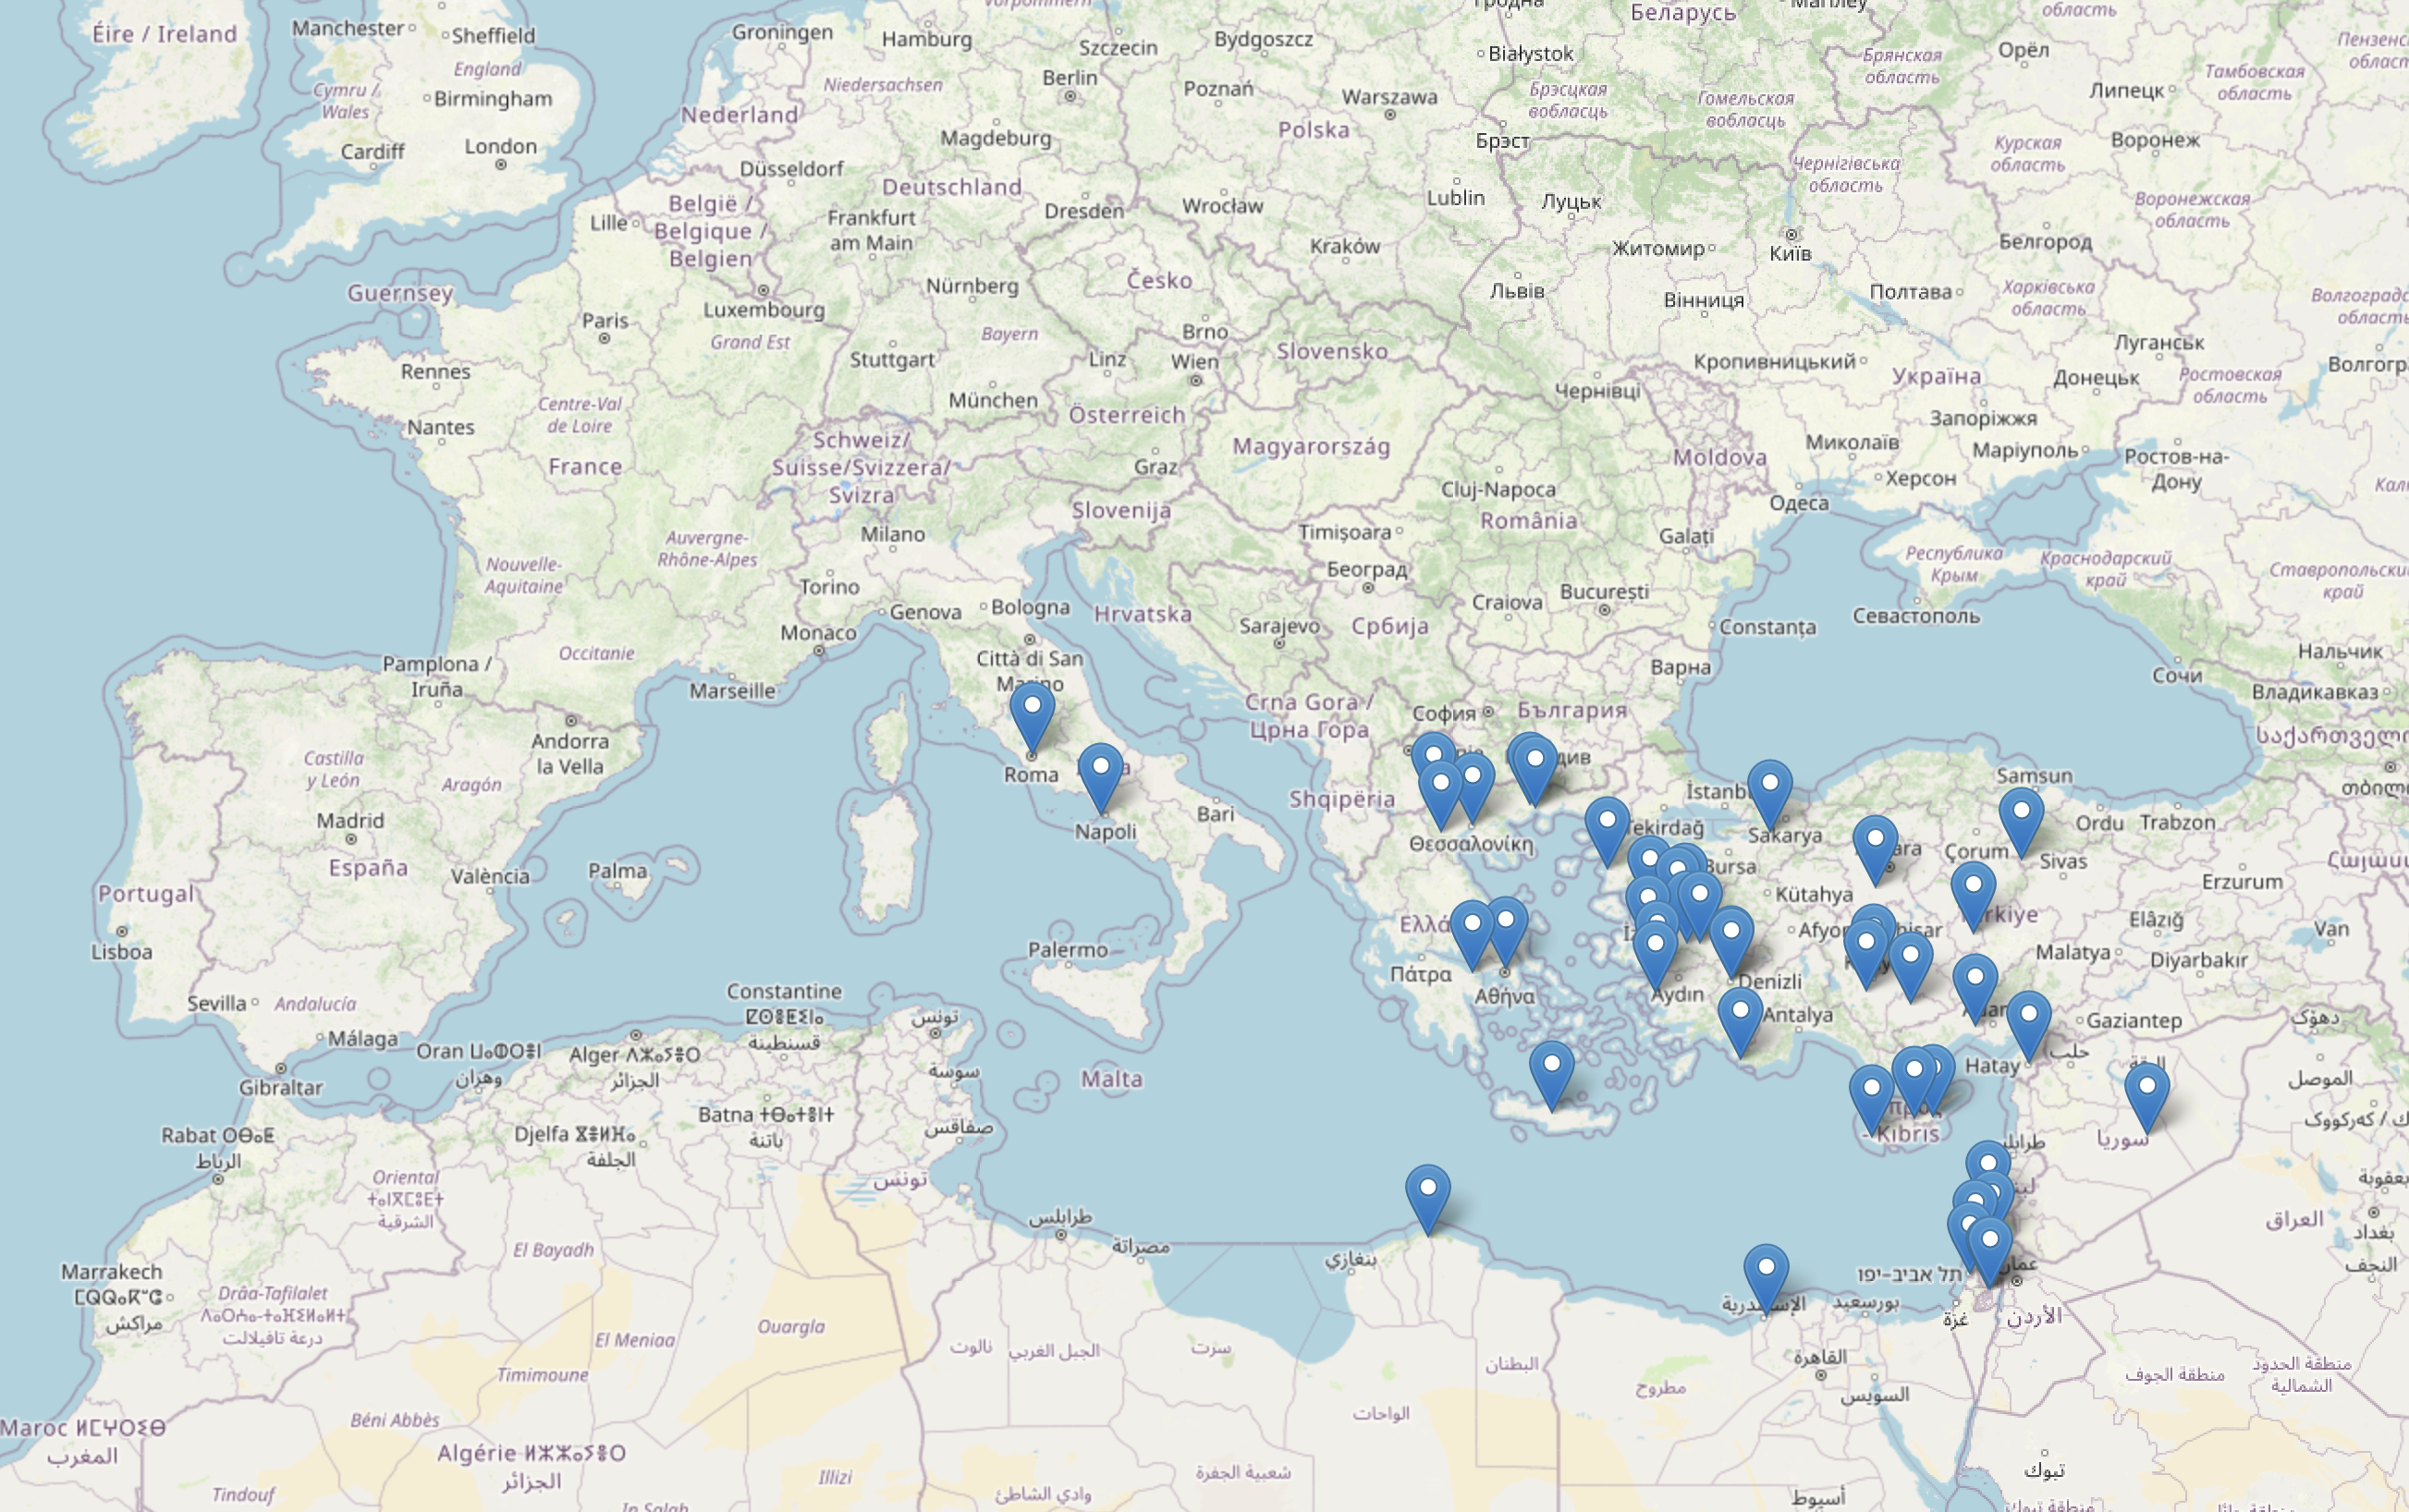
\includegraphics[width=\textwidth, keepaspectratio]{../../assets/locations_map}
    \caption{Mapa wszystkich lokalizacji wymienionych w Dziejach i listach.}
    \label{fig:figure}
\end{figure}

Osoby obeznane geograficznie dostrzegą niemal idealną korelację z granicami wschodniego cesarstwa rzymskiego.
Warto zwrócić uwagę na podróż do Rzymu, która miała zupełnie inny charakter niż pozostałe wyprawy.
\href{https://en.wikipedia.org/wiki/Byzantine_Empire_under_the_Theodosian_dynasty\#/media/File:4KTHEODOSIAN.png}{Mapa Rzymu}

\subsection{Uderzająca statystyka miast wymienionych w Dziejach i listach polega na tym, że wszystkie leżą w dawnym imperium greckim — i nie ma ani jednej wzmianki o mieście w imperium rzymskim, które nie należało wcześniej do imperium greckiego.}\label{subsec:the-striking-statistics-of-the-cities-mentioned-in-the-acts-and-the-epistles-are-that-they-are-all-in-the-former-greek-empire-and-not-one-mention-of-a-city-in-the-roman-empire-that-was-not-part-of-the-former-greek-empire.}

Ten fakt sprawia, że każda teoria uznająca chrześcijaństwo za ruch wyłącznie religijny, a nie polityczny, staje się natychmiast wysoce nieprawdopodobna.

\subsection{Minimalny opór wobec przyjęcia nowej religii.}\label{subsec:minimal-resistance-to-the-acceptance-of-the-new-religion.}

Nowa religia została przyjęta przez masy w dawnym imperium greckim i nie ma ani jednej wzmianki o oporze wobec niej ze strony samych Greków.
Jedyny realny sprzeciw pochodzi od władz świątynnych w Jerozolimie.
Jest to spójne z tezą, że chrześcijaństwo stanowi kontynuację greckiej filozofii imperialnej, którą ludność zhellenizowana już wcześniej akceptowała.

\subsection{Choć religia była tak skuteczna w pozyskiwaniu mas, zachowywała wszystkie elementy konspiracyjności.}\label{subsec:even-though-the-religion-was-so-successful-at-converting-the-masses-it-still-had-all-the-conspiratorial-parts-to-it.}

Pierwsi chrześcijanie używali tajnych symboli, by się rozpoznawać, spotykali się nocą, organizowali wspólne posiłki, posługiwali się zakodowaną ikonografią (ryba, kotwica, chi-rho) i unikali widoczności publicznej ze względu na wrażliwość polityczną.
Zarówno kult Mitry, jak i chrześcijaństwo funkcjonowały jako dyskretne, związkowe bractwa inicjacyjne związane przysięgą — różnica dotyczy treści teologicznej, a nie formy socjologicznej.
Pauline sformułowanie „żołnierze Chrystusa” idealnie wpisuje się w ten konspiracyjno-wojskowy model.

\subsection{Chrześcijaństwo było znacznie bardziej prześladowane niż jakakolwiek inna religia w imperium rzymskim.}\label{subsec:christianity-much-more-prosecuted-than-any-other-religion-in-the-roman-empire.}

Imperium rzymskie było bardzo tolerancyjne wobec innych kultów, a jedynym powodem ich ścigania było uznanie ich za zagrożenie dla państwa.
Chrześcijanie byli prześladowani nie za to, że czcili obcego boga, lecz za odmowę udziału w kulcie cesarskim przy równoczesnym twierdzeniu, że jedynie ich Chrystus jest królem.

Najpierw trzeba zauważyć, że najszerzej znane źródło o wczesnym prześladowaniu chrześcijan — oskarżenie Nerona, jakoby chrześcijanie wzniecili Wielki Pożar Rzymu — jest dziś powszechnie dyskredytowane jako zmyślenie.
Tacyt wspomina w swoim dziele o \emph{Chrestosie}, co było bardzo pospolitym imieniem i niemal na pewno nie odnosi się do Jezusa.
Pisząc po raz pierwszy o chrześcijanach, Tacyt — pięćdziesiąt lat po wydarzeniach — nie zna tej grupy.
To samo dotyczy Pliniusza Młodszego, który w swoim liście do Trajana również nie orientuje się, kim są chrześcijanie.
Gdyby chrześcijan obarczano winą za największą katastrofę w życiu zarówno Tacyta, jak i Pliniusza, byłoby nie do pomyślenia, by o tym nie wiedzieli.

Jednocześnie jednak Piotr został stracony w Rzymie przez ukrzyżowanie, a Paweł — przez ścięcie.
Podobnie jak w przypadku Jezusa, ukrzyżowanie było zarezerwowane dla zbrodni przeciw państwu, buntów i zdrady.
Jako obywatel rzymski Paweł został ścięty za te same przestępstwa.
Jeżeli nie istniały zorganizowane prześladowania chrześcijan, trudno wyjaśnić, dlaczego zarówno Piotr, jak i Paweł zostali zgładzeni w taki właśnie sposób.

\subsection{Określenie „żołnierze Chrystusa” nie pojawia się dosłownie w Ewangeliach, ale występuje wyraźnie w listach Pawła.}\label{subsec:the-phrase-soldiers-of-christ-is-not-used-explicitly-in-the-gospels-but-it-appears-prominently-in-the-pauline-epistles-particularly-in-the-context-of-the-christian-life-being-compared-to-a-military-struggle-or-a-spiritual-battle.}

W świecie rzymskim metafory wojskowe nigdy nie były tylko metaforami.
Autorzy rzymscy używali języka żołnierskiego wobec grup, które składały przysięgi, miały tajne lojalności, utrzymywały wewnętrzną dyscyplinę i działały w komórkach lub bractwach.
Cyceron nazywa spiskowców Katyliny „żołnierzami Katyliny” długo po tym, jak byli nieuzbrojeni (\emph{Filipiki} 13.27).
Józef Flawiusz opisuje zwolenników Judy Galilejczyka jako „zdyscyplinowanych jak żołnierze”, choć nie stanowili regularnej armii (\emph{Dawne Dzieje Izraela} 18.23).
Plutarch opisuje frakcje polityczne jako działające „jak żołnierze”, nawet bez broni (\emph{Żywot Sertoriusza} 26).
Ilekroć ruch był związany przysięgą lub nastawiony na zmianę ustroju, autorzy rzymscy spontanicznie sięgali po język żołnierski, nawet jeśli nie istniała otwarta armia.

Paweł intensywnie korzysta z tego słownictwa: στρατιώτης Χριστοῦ, „żołnierz Chrystusa” (2 Tm 2:3); συστρατιώτης, „współ-wojownik” (Flp 2:25; Flm 2); στρατεία, „kampania wojenna” (1 Kor 9:7; 2 Kor 10:3–4); πανοπλία, „pełna zbroja” (Ef 6:11).
Wszystkie te cztery terminy należą do sfery składania przysięgi, zdyscyplinowanego posłuszeństwa, gotowości do konfliktu i wspólnej walki.
Starożytny słuchacz, słysząc „żołnierze Chrystusa”, nie odbierałby tego jako miłej metafory.
Usłyszałby: to grupa lojalnościowa zorganizowana jak armia.

Rzymskie przesłuchania chrześcijan potwierdzają tę interpretację.
Pliniusz, Tacyt i \emph{Acta Scillitanorum} wielokrotnie zarzucają chrześcijanom nielegalne zgromadzenia, tajne przysięgi, odmowę udziału w kulcie cesarskim i przynależność do \emph{collegium illicitum}.
Rzymianie opisują ich jako grupy związane przysięgą i zdyscyplinowane — znacznie bliższe oddziałom żołnierskim niż dobrowolnym klubom kultowym.
Jeśli chrześcijanie otwarcie posługiwali się językiem żołnierskim, urzędnicy rzymscy traktowali to dosłownie.

Miasta Pawła — Filippi, Korynt, Tesalonika, Efez, Antiochia — wszystkie posiadały stałe lub półstałe garnizony rzymskie.
Kiedy Paweł nazywa zaufanych współpracowników „współ-wojownikami”, nadaje im standardowy rzymski tytuł dowódców komórek wewnątrz zorganizowanego ruchu.
Ma to pełny sens w świecie, w którym Jezus jest królem, królestwo jest realne, lojalność wobec Chrystusa koliduje z lojalnością wobec Cezara, a wierzący działają jak podziemna struktura przygotowująca się do przestawienia ładu politycznego.

\section{Wczesne datowanie Ewangelii może uczynić listy Pawła bardziej wiarygodnymi, ponieważ wydaje się, że Paweł zna przynajmniej jedną z Ewangelii oraz Dzieje Apostolskie.}\label{sec:the-early-dating-of-the-gospels-can-make-the-letters-of-paul-more-plausible-as-it-seems-paul-already-has-the-knowledge-of-at-least-one-of-the-gospels-and-the-acts.}

Wielu badaczy podaje w wątpliwość istnienie Pawła, opierając się na uderzającej sprzeczności w nurcie głównym: autorzy listów Pawłowych zdają się znać Ewangelie i Dzieje, a równocześnie Ewangelie i Dzieje są niemal jednomyślnie datowane na okres \emph{po} listach Pawła.
W tym ujęciu samo istnienie Pawła można ponownie przemyśleć, jeśli przyjmiemy wczesne datowanie Ewangelii i to, że Ewangelia Jana została napisana przez naocznego świadka życia Jezusa.

\subsection{Paweł ledwie wspomina o życiu Jezusa i prawie nigdy go nie cytuje.}\label{subsec:paul-barely-mentions-the-life-of-jesus-and-almost-never-quotes-him.}

Często twierdzi się, że religia Pawła nie jest religią Jezusa, lecz religią o Jezusie.
Uderza brak odniesień do jakichkolwiek nauk Jezusa, do prawa żydowskiego oraz do wydarzeń związanych z życiem i śmiercią Jezusa.
Możemy więc pójść o krok dalej.
Jest to religia skupiona na odnowieniu królestwa Bożego poprzez przywrócenie urzędu Christosa, prawowitego króla królestwa Bożego.
Dlatego dla Pawła i wszystkich wczesnych chrześcijan chodziło przede wszystkim o przywrócenie Chrystosa, a nie o nauczanie konkretnego Jezusa Chrystusa.
Chodziło o to, że Bóg ponownie pośle króla, który odnowi imperium greckie — królestwo Boże — pod przewodnictwem Christosa, prawowitego ziemskiego króla królestwa Bożego.

\subsection{Używanie tego języka konspiracyjnego jasno zadziałało.}\label{subsec:using-this-conspiratorial-language-clearly-worked}

Rzym nawet nie zorientował się, że celem nowej religii jest przywrócenie Wschodniego Imperium, dopóki to faktycznie nie nastąpiło.

\subsection{10.
Aleksandria była stolicą imperium greckiego i centrum świata hellenistycznego, a jednak nie ma żadnych misji ani listów skierowanych do Aleksandrii.}

\label{subsec:alexandria-was-the-capital-of-the-greek-empire-and-the-center-of-the-hellenistic-world-and-yet-there-are-no-missions-or-letters-to-alexandria.}

Nieobecność Aleksandrii w Nowym Testamencie jest uderzająca, zwłaszcza jeśli uwzględnić jej znaczenie.
Aleksandria została z tekstu usunięta, choć była miastem pochodzenia Apollosa oraz niektórych innych towarzyszy Pawła, takich jak Marek, Demas i Łukasz.
To przemilczenie najlepiej wyjaśnić jako celowe wymazanie, właśnie dlatego, że Aleksandria była już centrum ruchu.
Tak jak Stary Testament w dużej mierze pomija imperium Ptolemejskie mimo jego centralnego znaczenia, tak Nowy Testament minimalizuje rolę Aleksandrii, jednocześnie zakładając jej przywództwo.

\section{Dzieje Apostolskie}\label{subsec:acts-of-the-apostles}

Nazywają się Dzieje \emph{Apostolskich}, a nie dzieje uczniów.
Apostołowie wykonują pracę imperialną: ogłaszają wszystkim narodom imperium wolę Boga-Króla.

\subsection{10.
Dzieje rozpoczynają się od królewskiej intronizacji}\label{subsec:acts-opens-with-a-royal-enthronement}

Dz 1:6 --- „Panie, czy w tym czasie odbudujesz królestwo Izraela?”.
To nie jest pytanie duchowe.
Zakłada, że Jezus rości sobie prawo do politycznego królowania.
Twoja teoria: Jezusa postrzegano jako prawowitego monarchę odnowionego królestwa — następcę tronów herodiańskich lub hasmonejskich w ramach greckich ideałów imperialnych.

\subsection{10.
Jezus zostaje wzięty do nieba jak cesarz}\label{subsec:jesus-is-taken-up-like-an-emperor}

Dz 1:9–11 --- Wniebowstąpienie naśladuje sceny apoteozy (np. Aleksandra, cesarzy rzymskich).
Przedstawia Jezusa w kategoriach imperialnych, jako wyniesionego na tron w niebie — jak boskiego cesarza.
To dokładnie odpowiada ujęciu, że chrześcijaństwo dotyczyło lojalności wobec „Chrystusa-Cesarza”.

\subsection{10.
Scena Pięćdziesiątnicy naśladuje inaugurację imperialną}\label{subsec:the-pentecost-scene-mimics-an-imperial-inauguration}

Dz 2 --- Cud wielojęzyczności i masowego nawrócenia odzwierciedla imperialny ideał zjednoczenia narodów pod jednym boskim królem.
Język „języków” ma wymiar polityczny: przesłanie cesarza jest przeznaczone dla wszystkich narodów.

\subsection{10.
Dz 5: proces apostołów}\label{subsec:acts-5-the-trial-of-the-apostles}

Gamaliel przywołuje wcześniejszych przywódców rewolucyjnych — Teudasa i Judę Galilejczyka.
Potwierdza w ten sposób, że mesjańskie bunty miały charakter polityczny i że ruch Jezusa był postrzegany w podobnych kategoriach.

\subsection{10.
Mowa Szczepana w Dz 7 jest anty-świątynna}\label{subsec:stephens-speech-in-acts-7-is-anti-temple}

Szczepan atakuje Świątynię i tradycję Mojżeszową, nawiązując do krytyki legalizmu żydowskiego u Filona i myślicieli stoickich.
Wspiera to pogląd, że wczesne chrześcijaństwo odrzucało religię Mojżeszową i było bliższe filozoficznemu monoteizmowi.

\subsection{10.
Dzieje kończą się bez rozwiązania akcji}\label{subsec:acts-ends-without-resolution}

Księga kończy się w Rzymie, gdzie Paweł swobodnie głosi „królestwo Boże”.
Brakuje narracyjnego finału, ponieważ prawdziwe przesłanie brzmi: imperium jest już chrześcijańskie.
Zakłada to istniejącą wcześniej publiczność, która widzi chrześcijaństwo jako siłę polityczno-teologiczną.

\subsubsection{Jakub Sprawiedliwy}\label{subsec:james-the-just}

\subsection{Jakub Sprawiedliwy również napisał list do wszystkich narodów.}\label{subsec:james-the-just-also-wrote-an-epistle-to-all-nations.}

Był bratem Jezusa i kolejnym w linii dziedziczenia tronu.
Podobnie jak Jezus Chrystus Zbawca, Jakub nosił tytuł królewski: Sprawiedliwy.

Jakub Sprawiedliwy również napisał list do wszystkich narodów, włączony do Nowego Testamentu.
Jakub, podobnie jak Jan, odwołuje się do tego samego rozumienia Logosu co Filon z Aleksandrii.
Styl retoryczny Jakuba — moralna diatryba z wyimaginowanymi rozmówcami, wezwania w trybie rozkazującym, żywe przykłady — należy do tego samego hellenistycznego nurtu filozoficznej nauki moralnej, który przejął Filon.

Po grecku Jk 1:21 brzmi:
„Διὸ ἀποθέμενοι πάσαν ἀκαθαρσίαν καὶ περισσείαν κακίας ἐν πραΰτητι δέξασθε τὸν ἐμφυτον λόγον, ὃς δύναται σῶσαι τὰς ψυχὰς ὑμῶν.”
Transliteracja: „Dio apothemenoi pasan akatharsian kai perisseian kakias en prautēti dexasthe ton emphuton logon, hos dynatai sōsai tas psychas hymōn.”
Przekład dosłowny: „Dlatego, odrzuciwszy wszelką nieczystość i nadmiar zła, w łagodności przyjmijcie wszczepione słowo, które może zbawić wasze dusze.”

List Jakuba jest napisany wyrafinowaną literacką koine, z użyciem złożonych zdań podrzędnie złożonych, szerokiego i częściowo twórczego słownictwa (zawiera ponad sześćdziesiąt słów unikatowych w Nowym Testamencie) oraz technik retorycznych hellenistycznej diatryby moralnej — paronomazji, aliteracji, personifikacji i gwałtownych pytań retorycznych.
Taki poziom greki trudno pogodzić z analfabetą-parobkiem wiejskim i wskazuje raczej na postać osadzoną w wykształconych, greckojęzycznych sieciach wschodniego basenu Morza Śródziemnego, czy to dzięki własnej formacji, czy we współpracy z biegłym skrybą.

\subsubsection{Listy Jana}\label{subsec:the-epistles-of-john}

\subsection{Obalenie istniejących modeli}\label{subsec:a-disproof-of-existing-models}

Literatura naukowa zwykle wyjaśnia powstanie chrześcijaństwa w ramach jednego z trzech modeli: misyjnej dyfuzji, żydowskiej sekty lub konkurencji kultów imperialnych.
Wszystkie trzy zakładają, że chrześcijaństwo rozpoczęło się jako mała grupa religijna i stopniowo rozszerzało poprzez procesy organiczne.
Rzeczywiste dane pokazują, że to założenie jest niemożliwe.

\textbf{1. Model misyjnej dyfuzji (Harnack, Stark i in.).}
Model ten wyobraża sobie apostołów podróżujących od miasta do miasta, nawracających domy i zakładających lokalne wspólnoty, które następnie rosły z czasem.
Przewiduje on: (a) stopniowe rozprzestrzenianie się po regionach, (b) nierównomierną recepcję, (c) wielojęzyczną dokumentację oraz (d) ciągły wzrost w II wieku.
\emph{Obserwacja:} nagła sieć kościołów w każdym większym polis greckiego Wschodu, wyłącznie w języku greckim, po czym następuje stulecie stagnacji.
\emph{Wniosek:} model nie jest w stanie tego wyjaśnić.
Stopniowa dyfuzja nie daje w efekcie natychmiastowej obecności w całym imperium, a potem ciszy.

\textbf{2. Model żydowskiej sekty (Eisenman, Sanders, Vermes i in.).}
Model ten opisuje chrześcijaństwo jako mesjańską reformę wewnątrz judaizmu, która dopiero później otworzyła się na pogan.
Przewiduje: (a) najwcześniejsze pisma w języku aramejskim lub hebrajskim, (b) oparcie na prawie Mojżeszowym i tradycji świątynnej, (c) ekspansję poprzez diasporę synagogalną oraz (d) późniejsze tłumaczenia na grekę.
\emph{Obserwacja:} ani jednego listu po aramejsku czy hebrajsku, brak rozprzestrzeniania się przez synagogi, wrogość wobec prawa Mojżeszowego i powszechna korespondencja w języku greckim.
\emph{Wniosek:} oczekiwane żydowskie ramy są całkowicie nieobecne.
Ruch jest grecki i imperialny od samego początku.

\textbf{3. Model konkurencji kultów imperialnych (Friesen, Harland i in.).}
Model ten ujmuje chrześcijaństwo jako kolejny kult miejski konkurujący na rzymskim rynku religijnym.
Przewiduje: (a) stopniowe przyjmowanie zarówno na łacińskim Zachodzie, jak i na greckim Wschodzie, (b) lokalną różnorodność praktyk, (c) synkretyzm z kultem cesarskim oraz (d) powolny wzrost od prywatnych stowarzyszeń do kultu publicznego.
\emph{Obserwacja:} brak ekspansji na łaciński Zachód, brak losowego rozproszenia po miastach rzymskich, za to pełne pokrycie dawnego imperium greckiego z jednolitym roszczeniem jednego królewskiego Chrystosa.
\emph{Wniosek:} dane obalają ten model.
Zamiast rozproszonej konkurencji kultów, widzimy wzorzec spójny i scentralizowany.

\textbf{Ostateczna ocena.}
Każdy z modeli alternatywnych się załamuje.
Ich przewidywania nie tylko „słabo pasują” — są całkowicie nie do pogodzenia z rzeczywistymi świadectwami.
Jest więc pewne, że wczesne chrześcijaństwo nie było produktem misyjnego wzrostu, żydowskiego sekciarstwa ani konkurencji kultów.
Kościoły nie były świeżo zakładanymi zgromadzeniami, lecz kontynuującymi działalność \textit{ekklesiami} świata greckiego, przeorganizowanymi pod panowaniem Christosa.
Sekwencja wydarzeń — brak obecności, natychmiastowe pokrycie imperialne, potem długotrwała stagnacja — dopuszcza tylko jedno wyjaśnienie: kontynuację imperium greckiego pod nową proklamacją królewską.

\subsection{Korpus Nowego Testamentu}\label{subsec:the-corpus-of-the-new-testament}

Co tak naprawdę wchodzi w skład Nowego Testamentu i jak rozkłada się to na cztery bieguny imperialne, które zidentyfikowaliśmy?
Poniżej czynimy tę mapę jawną \emph{oraz} kotwiczymy ją w konkretnych starożytnych świadectwach, zwłaszcza w odniesieniu do listów i wczesnych twierdzeń o autorstwie.
Warto podkreślić: w starożytności przypisania czterech kanonicznych Ewangelii \textit{Mateusz, Marek, Łukasz, Jan} są jednomyślnie podtrzymywane przez Ojców.
Nie zanotowano dla nich żadnych alternatywnych apostolskich imion.

\subsection{Świadectwa patrystyczne (autorstwo w starożytności).}

Przed połową III wieku obraz jest spójny.
\textbf{Papias} (przez Euzebiusza, \textit{Hist.\ Eccl.} 3.39) — Marek pisał jako tłumacz Piotra.
Mateusz zebrał \textit{logia}.
\textbf{Ireneusz} (\textit{Adv.\ Haer.} 3.1.1) — wprost wylicza i broni czterech: Mateusza, Marka, Łukasza (towarzysza Pawła) i Jana.
\textbf{Fragment Muratoriański} (koniec II w.) nazywa Łukasza i Jana trzecim i czwartym ewangelistą i rozpoznaje korpus Pawłowy.
\textbf{Klemens Aleksandryjski} i \textbf{Orygenes} powtarzają te przypisania.
\textbf{Euzebiusz} później podsumowuje je jako powszechnie przyjęte.
Co do listów: \textbf{1 List Klemensa} (ok. 96 r.) cytuje 1 List do Koryntian.
\textbf{Ignacy} (ok. 110 r.) zakłada istnienie kościołów pawłowych i ich języka.
\textbf{Polikarp} (ok. 135 r.) cytuje lub parafrazuje wiele listów Pawła i 1 List Piotra.
\textbf{Ireneusz} korzysta z 1–2 Listu Piotra, 1 Listu Jana i Listu Jakuba jako pism apostolskich.
Dyskusje nad autorstwem Listu do Hebrajczyków i późnością 2 Listu Piotra pojawiają się dopiero później.
Kluczowe jest to, że nie ma wczesnych kontrprzypisań \emph{czterech Ewangelii} do innych imion.

\subsection{Papirologia i wczesny obieg (migawka).}

\textbf{P\textsuperscript{46}} (ok. 200 r.) zawiera zbiór listów Pawła (Rz, 1–2 Kor, Ga, Ef/Kol, Flp, 1 Tes, Hbr), pokazując, że listy krążyły już jako korpus.
\textbf{P\textsuperscript{66}} (ok. 200 r.) i \textbf{P\textsuperscript{75}} (początek III w.) to główne wczesne świadectwa Ewangelii Jana (oraz Łukasza/Jana).
\textbf{P\textsuperscript{9}} (III w.) zachowuje fragment 1 Listu Jana z Oksyrynchos.
\textbf{P\textsuperscript{72}} (III/IV w.) zawiera 1–2 List Piotra i List Judy.
\textbf{P\textsuperscript{13}} (III w.) — List do Hebrajczyków.
\textbf{P\textsuperscript{45}} (III w.) — Ewangelie/Dzieje.
Świadectwa te potwierdzają wczesny obieg i naturalne klastrowanie (zestaw Pawłowy; Piotrowy/Judy; Janowy), które odzwierciedla naszą czterobiegunową architekturę.
Egipskie miejsca znalezienia odzwierciedlają stronniczość zachowania materiału.
\emph{Kompozycyjne} skupiska nadal odpowiadają mapie imperialnej.

\subsection{Cztery ocalałe greckie światy kulturowe po Aleksandrze}

Istnienie czterech kanonicznych Ewangelii nie było późniejszym redakcyjnym przypadkiem ani teologicznym kompromisem.
Odzwierciedla coś znacznie starszego i głębszego: sam wschodni basen Morza Śródziemnego był ustrukturyzowany w cztery wielkie światy kulturowe, które przetrwały w niezmienionej formie od czasu rozpadu imperium Aleksandra.
Ewangelie powstały wewnątrz tego czteroczłonowego świata, a ich różnice odzwierciedlają właśnie te cztery ocalałe greckie sfery kulturowe.

Gdy imperium Aleksandra się rozpadło, nie rozkruszyło się na dziesiątki równorzędnych państw; niemal natychmiast skrystalizowało się w cztery dominujące regiony dynastyczne, z których każdy stał się samowystarczalnym ekosystemem kulturowym, z własnymi instytucjami, własnym idiomem greckim i własną pamięcią polityczną.
Nie były to jedynie królestwa w sensie politycznym; były to całe cywilizacyjne światy, każdy na tyle rozległy, by kształtować życie milionów ludzi, i na tyle stabilny, by trwać przez stulecia, nawet po zniknięciu samych dynastii.
Każde ważniejsze miasto, każdy lud i każdy system edukacyjny we wschodnim basenie Morza Śródziemnego należał do jednego z tych czterech światów.

Ptolemejska Egipt zbudował najbardziej intelektualnie ambitną kulturę grecką starożytności.
Aleksandria pozostała bezdyskusyjnym centrum badań, żydowsko–greckiej syntezy filozoficznej, produkcji tekstów i spekulacji metafizycznej, nawet po tym jak August przyłączył Egipt do imperium.
Jej instytucje przeżyły dynastię: Muzeum, akademie filozoficzne, kultura skrybów oraz charakterystycznie aleksandryjski styl greki pojęciowej przetrwały w stanie nienaruszonym.
To właśnie ten świat wydał teologię Logosu, dualizmy platońskie, dialogi objawieniowe i słownik metafizyczny, które znamionują Ewangelię Jana.
Jan nie jest anomalią; to głos judaizmu aleksandryjskiego, mówiącego po grecku w swoim własnym intelektualnym rejestrze.

Seleucka Syria, z Antiochią jako stolicą, rozwinęła zupełnie inne greckie środowisko: grecką metropolię na skraju aramejskojęzycznego zaplecza.
Rzeczywistość językowa tego regionu była stabilna i jednoznaczna — greka w miastach, aramejski na prowincji — co tworzyło naturalny, niewymuszony bilingwizm.
Krótkie rozkazy, przezwiska, okrzyki, formuły uzdrowień i pograniczne zwroty nieustannie przechodziły z jednego języka do drugiego.
Dokładnie taki wzorzec zachowuje się w aramejskich zwrotach Marka.
Nie są to relikty galilejskiego Jezusa; to nawyki kodowego przełączania się językowego greckiego autora z Antiochii, piszącego wewnątrz syryjsko–seleuckiego świata dwujęzycznego.
Heroiczny styl pogranicza, urywana narracja, epicko–mimetyczna struktura i mieszanka greki z aramejskim doskonale pasują do Antiochii, a wcale do Galilei.

Królestwo Judei, stworzone przez Hasmoneuszy na długo przed wejściem Rzymu do regionu, było projektem dużego, spójnego, politycznie ambitnego ludu, zdeterminowanego, by rządzić sobą samym.
Nie było wytworem Rzymian.
Zdobyli niezależność, ponieważ w momencie załamania władzy Seleucydów byli wystarczająco silni i dobrze zorganizowani, by stworzyć własną dynastię i zachować własne tradycje w obrębie greckiej oikoumene.
Herodiańscy następcy kontynuowali ten świat w innym tonie, ale blok kulturowy trwał: region z własnymi szkołami prawa, własną pamięcią dynastyczną, własnymi sporami o legitymizację i własną tożsamością w ramach greckiej kultury politycznej.
Ewangelia Mateusza odzwierciedla to środowisko z niezwykłą precyzją: genealogia dynastyczna, argumentacja prawno–egzegetyczna, formuły wypełnienia proroctw i judejska teologia polityczna wyrażona po grecku, a nie egejski styl retoryczny, ani aleksandryjski styl metafizyczny, ani syryjski styl bilingwalny.

Świat Antygonidów — Macedonia, Grecja i basen Morza Egejskiego — był czwartym wielkim postaleksandryjskim kręgiem kulturowym.
Nawet po zgnieceniu samej dynastii instytucje, które zbudowała, przetrwały w niezmienionej formie.
Gimnazja, szkoły retoryki klasycznej, zgromadzenia polis, dekrety honorowe, tradycja historiografii elit i system edukacyjny greckiego lądu oraz zachodniej Azji Mniejszej wszystkie wywodziły się z fundamentów antygonidzkich.
W I wieku Efez stał się faktyczną metropolią całego tego regionu: największym, najbogatszym, najbardziej „instytucjonalnie greckim” miastem świata egejskiego.
To właśnie ten krąg kulturowy wydał Saloniki, Filippi, Korynt i szerszą, miejską sieć pawłową.
To także sfera odzwierciedlona w grece Łukasza: wyszlifowany proem historiograficzny, precyzja administracyjna, słownictwo żeglarskie, terminologia miejska i struktura retoryczna nauczana w gimnazjach egejskich.
Łukasz nie pisze „ogólnej” greki; pisze greką klasycznego centrum edukacyjnego całego Morza Śródziemnego.

Te cztery światy były jedynymi realnymi, wielkoskalowymi podziałami kulturowymi greckiego Wschodu.
Każdy inny podział jest sztuczny.
Każdy region podpadał pod któryś z tych bloków.
Ich kultury instytucjonalne przetrwały długo po tym, jak dynastie przestały rządzić.
Pod rzymską administracją te cztery światy nadal istniały jako fakty kulturowe: Aleksandria myślała jak Ptolemeusze, Antiochia jak Seleucydzi, Jerozolima jak jej rodzima dynastia, a miasta egejskie jak świat Antygonidów.

Dlatego właśnie różnorodność Ewangelii wreszcie nabiera historycznego sensu.
Każda Ewangelia nie jest tylko portretem teologicznym; jest wytworem jednego z tych czterech wielkich ekosystemów kulturowych.
Jan przemawia z Aleksandrii.
Marek przemawia z Antiochii.
Mateusz przemawia z Judei.
Łukasz przemawia ze świata egejskiego.
Czterokrotna Ewangelia nie jest przypadkiem powstania kanonu; jest literacką mapą czterech ocalałych kultur greckich wschodniego basenu Morza Śródziemnego.
Sama struktura czterokrotna jest jednak starsza niż Aleksander.

\subsection{Cztery symbole królewskie sprzed Aleksandra}

Czteropolowa mapa, która kształtuje Ewangelie, nie została wymyślona w epoce hellenistycznej.
Czytelnik natychmiast zauważy, że Ezechiel prorokował w VI wieku p.n.e., na długo przed rozbiciem imperium Aleksandra na Ptolemeuszy, Seleucydów, Hasmoneuszy i Antygonidów.
Ten dystans chronologiczny nie stanowi problemu; jest kluczem.
Widzenie Ezechiela należy do świata, w którym Bliski Wschód używał czterech symboli królewskich od ponad tysiąca lat.
Symbole te nie były ozdobą.
Były oficjalnymi insygniami państwowymi, znakami wojskowymi, ikonami świątynnymi i emblematami królewskimi czterech wielkich sfer kulturowych, które poprzedzały wszystkie późniejsze imperia.
Gdy Ezechiel widzi lwa, wołu, orła i człowieka, opisuje ugruntowaną polityczną i kosmologiczną gramatykę starożytnego Bliskiego Wschodu — sposób, w jaki królestwa przedstawiały władzę.
Te cztery emblematy stoją w centrum politycznej teologii regionu na długo przed Ewangeliami i na długo przed rządami hellenistycznymi.

Przez ponad dwa tysiące lat przed Ezechielem symbolem królewskości Egiptu był koronowany sokół Horusa, umieszczony nad imieniem królewskim w każdej kartuszy.
Każdy faraon od Starego Państwa w górę był explicite tytułowany „Horus”, a ptak–sokół pojawiał się na znakach wojskowych, fasadach pałacowych, świątyniach grobowych, chorągwiach wojskowych i w biżuterii królewskiej.
W Okresie Późnym — za życia samego Ezechiela — sokół pozostawał oficjalnym emblematem egipskiej suwerenności, widocznym w ikonografii tronu, w szatach kapłańskich i na reliefach monumentalnych.
Dlatego oblicze orła u Ezechiela jest natychmiast rozpoznawalne: przywołuje wschodni symbol boskiego królowania, stworzenie, które dosłownie spoczywa na głowie każdego faraona jako duet ureus–Horus.
Gdy Ptolemeusze później rządzą Egiptem, przyjmują Orła Zeusa, będącego po prostu greckim odpowiednikiem sokoła Horusa: królewskiego ptaka nieba, emblemat suwerenności.
Symbol ten jest tak dominujący, że staje się rzymskim orłem legionowym, a przez Rzym przechodzi w emblemat Bizancjum, Niemców, Rosjan, Polaków, Amerykanów i republik arabskich.
Orzeł jest najstarszym nieprzerwanym symbolem królewskim wschodniego basenu Morza Śródziemnego i politycznym obliczem wschodniego kwadrantu starożytnego świata.

We wschodnim Lewancie — świecie fenickim i aramejskim — wół był najwyższym symbolem władzy państwowej przez co najmniej tysiąc lat przed Aleksandrem.
Wół był żywym emblematem Baala i Hadada, królewskiego boga burzy tego regionu, który w tekstach ugaryckich z XIII–XII wieku p.n.e. zasiada na tronie na grzbiecie wołu, włada deszczem i legitymizuje królów.
Fenickie świątynie w Byblos, Tyrze i Sydonie wystawiały przy bramach brązowe woły; miasta aramejskie rzeźbiły posągi wołów jako figury strażnicze; królewskie pieczęcie w całym Kanaanie przedstawiają bóstwa o głowach wołów przekazujące władzę królom.
Gdy Biblia opisuje, że Izrael buduje złotego cielca, nie mówi o przypadkowym bożku — opisuje oficjalnego fenickiego boga państwowego, królewski emblemat całego systemu monarchii nadbrzeżnych.
W czasach Ezechiela wół jest już rozpoznawalnym symbolem zachodniego kwadrantu, rolniczo–morskiego świata rządzonego przez bogów burzy.
Gdy Seleucydzi później budują swoje imperium na tym samym obszarze, przyjmują hybrydę wołu, konia i rogatej ikonografii mocy, która kontynuuje ten liczący tysiąclecia emblemat władzy.
Ox face Ezechiela nie jest więc zwierzęciem wybranym losowo; to polityczny symbol całego zachodniego bloku lewantyńsko–syryjskiego.

Na długo przed Ezechielem lew stał się kanonicznym emblematem królewskości w całym wnętrzu świata zachodniosemickiego, od Kanaanu i Moabu po Izrael i Judę.
Pałace asyryjskie pokrywają się niekończącymi się reliefami polowań na lwy, ponieważ lew symbolizował królewską dominację, a Babilon wznosi całe aleje lwów na potrzeby rytuałów państwowych.
Biblijny „Lew Judy” nie jest uroczą metaforą: to judejski emblemat państwowy poświadczony w ideologii królewskiej co najmniej od czasów Dawida, wzmocniony w błogosławieństwie Judy w Rdz 49 i wsparty ikonografią lwa na pieczęciach judejskich, dzbanach magazynowych i architekturze monumentalnej.
Potęga lwa nad pustynią, jego drapieżna gwałtowność i związek z królewskim podbojem uczyniły go naturalnym symbolem południowego kwadrantu: wyżyn zachodniosemickich i pustyń pogranicza.
W świecie Ezechiela lew pełni już funkcję identyfikatora królewskiej linii Izraela, tak jak sokół identyfikuje Egipt, a wół Fenicję.
Lew Ezechiela reprezentuje więc południową kulturę królewską na symbolicznej mapie Bliskiego Wschodu.

Czwarty symbol — człowiek — nie ma być słaby ani neutralny.
To człowiek heroiczny, postać dominująca w sztuce greckiej od epoki brązu.
Freski i kratery mykeńskie ukazują wojowników w hełmach; ceramika okresu geometrycznego przedstawia szeregi hoplitów; rzeźba archaiczna rozwija kurosa jako idealnego obywatela–wojownika; a klasyczne Ateny, Sparta i Macedonia czynią z uzbrojonej postaci ludzkiej podstawowy emblemat tożsamości obywatelskiej.
Świat grecki jest jedynym blokiem kulturowym Bliskiego Wschodu, którego symbol suwerena jest jawnie antropiczny: Achilles, Ajas, Herakles, Perseusz, Tezeusz i ostatecznie obywatel–hoplita.
Przez co najmniej siedem stuleci przed Ezechielem teologia polityczna świata egejskiego buduje się wokół człowieka–herosa, a nie zwierzęcego bóstwa.
Dlatego czwarta twarz Ezechiela — ludzka — należy do północnego kwadrantu, gór i miast–państw Anatolii i Grecji.
Gdy Aleksander rozszerza Grecję w imperium, nie tworzy tej tożsamości; globalizuje to, co już było ludzkim, heroicznym emblematem greckiego panowania.

W czasach, gdy Ezechiel pisze w VI wieku p.n.e., te cztery insygnia dominują w regionie już od ponad tysiąca lat: sokół jako symbol królewskości Egiptu, wół jako znak władzy Fenicji i Syrii, lew jako emblemat królewski Judy i świata zachodniosemickiego oraz człowiek–heros jako znak państw wojowniczych Anatolii i Grecji.
Jego czterotwarzowe stworzenie jest najstarszą zachowaną literacką reprezentacją czteroczłonowego świata bliskowschodniego, łączącą cztery symbole królewskie, cztery bloki kulturowe, cztery wiatry, czterech nosicieli tronu i czteroczłonową strukturę kosmosu.
Gdy Kościół pierwotny później mówi, że Ewangelia musi być czterokrotna, ponieważ świat jest czterokrotny, nie popada w mistykę.
Przypomina sobie tę starożytną symboliczną architekturę — taką, która poprzedza Aleksandra, poprzedza monarchię Izraela i poprzedza samego Ezechiela.
A gdy cztery kanoniczne Ewangelie trafiają w ręce Aleksandrii, Judei, Syrii i świata egejskiego, wchodzą bezpośrednio w czterokwadrantowy system świata, który był wizualnie i politycznie definiowany przez co najmniej tysiąc lat przez sokoła, wołu, lwa i herosa.

\subsection{Dlaczego Ireneusz się nie mylił}

Najwcześniejszym chrześcijaninem, który wyjaśnia, dlaczego istnieją cztery Ewangelie, jest Ireneusz, i podaje on powód, z którego niemal wszyscy dziś kpią: Ewangelie odpowiadają czterem istotom żyjącym — lew, wół, orzeł, człowiek — tym samym czterem istotom z Ezechiela i Apokalipsy.
Uczeni odrzucają to jako numerologię.
Traktują je jako mistyczną ozdobę albo prymitywną symbolikę.
Ale takie odrzucenie jest całkowicie powierzchowne.
Ireneusz nie wybiera zwierząt na chybił trafił.
Czerpie z sztywnej, odziedziczonej kosmologii czterech kierunków — tej samej symbolicznej architektury, której używa starożytna literatura apokaliptyczna — a ta czterostronna struktura jest dokładnie sposobem, w jaki świat śródziemnomorski po Aleksandrze był faktycznie podzielony.
Język symboliczny Ireneusza nakłada się bezpośrednio na realną rzeczywistość geopolityczną.

Ireneusz nie był osamotniony.
Schema czterech stworzeń przenika całą tradycję patrystyczną.
Apokalipsa jest pierwszym chrześcijańskim tekstem, który podejmuje wizję tronu z Księgi Ezechiela i czyni ją centralnym elementem chrześcijańskiej kosmologii: Jan opisuje cztery istoty żyjące „pośrodku tronu i dokoła tronu” (Ap 4,6–8), każdą z inną twarzą — lwa, cielca, człowieka, orła — śpiewające bez wytchnienia Trisagion, dokładnie tak jak cherubini Ezechiela wyznaczali obecność chwały Boga.
Już w Nowym Testamencie czterokrotna istota Ezechiela staje się częścią chrześcijańskiej gramatyki kosmosu i tronu, a nie marginalną ciekawostką.

Pod koniec II wieku Ireneusz czyni tę gramatykę explicite i kanoniczną.
W \textit{Against Heresies} 3.11.8 bierze istoty żyjące z Apokalipsy 4,7 i odczytuje je jako figury całej „ekonomii” Syna Bożego, po czym stwierdza wprost, że „istoty żyjące są czteroformne, Ewangelia jest czteroformna i droga, którą kroczył Pan, jest czteroformna”.
Dla Ireneusza nie chodzi o ładną alegorię, ale o konieczność: Kościół jest rozproszony po czterech wiatrach, świat ma cztery strefy i cztery główne wiatry, a zatem jeden Chrystus musi być głoszony w formie czterokrotnej, jeśli orędzie ma odpowiadać strukturze stworzenia.

Pisarze III wieku wzmacniają tę logikę.
Orygenes, w homiliach do Ezechiela i Łukasza, traktuje liczbę cztery jako immanentną tradycji Ewangelii, wiążąc ją z czterema rzekami Edenu, czterema wiatrami i czterema krańcami ziemi, i po prostu zakłada, że istoty Ezechiela i Jana dostarczają podstawowego schematu tego, jak jeden Chrystus może zostać przedstawiony w wielu, niekonkurujących formach.
Wiktoryn z Patawii, najwcześniejszy zachowany komentator Apokalipsy, jest jeszcze bardziej bezpośredni: komentując Apokalipsę 4 pisze, że „cztery istoty żyjące to cztery Ewangelie” i przypisuje każdej stworzonej istocie jednego ewangelistę, nalegając przy tym, że razem otaczają tron i śpiewają Trisagion.
Na tym etapie identyfikacja jest już ustalona: ilekroć prawowierni chrześcijanie czytają tron z Apokalipsy, widzą wokół niego rozchodzącą się kanoniczną czterokrotną Ewangelię.

Teologia łacińska IV i V wieku przejmuje to i buduje na tym ortodoksję.
Augustyn poświęca cały rozdział w \textit{De Consensu Evangelistarum} „czterem istotom żyjącym w Apokalipsie, które zostały uznane za trafne figury czterech ewangelistów”, przyjmuje identyfikację jako oczywistą i debatuje jedynie nad tym, które stworzenie najlepiej odpowiada któremu ewangeliście.
Dla Augustyna tetramorf oznacza, że ewangeliści różnią się, a zarazem są zgodni, tak jak cztery oblicza mogą należeć do jednego rydwanu–tronu: struktura czterech nie jest przypadkiem przetrwania rękopisów, lecz znakiem, że Duch rozdzielił jedną rzeczywistość chrystologiczną na cztery komplementarne perspektywy.
Hieronim w swoich przedmowach i komentarzu do Mateusza standaryzuje dobrze nam dziś znany zachodni przydział — człowiek dla Mateusza, lew dla Marka, wół dla Łukasza, orzeł dla Jana — i scala go z kolejnością w Wulgacie, która zdominuje sztukę i liturgię średniowiecza.
Późniejsi pisarze łacińscy, tacy jak Chromacjusz czy Raban Maur, po prostu powtarzają ten schemat: cztery istoty żyjące, cztery wiatry, cztery krańce ziemi, czterej ewangeliści, jeden tron.

Kluczowe spostrzeżenie jest takie, że wszyscy ci autorzy nie zgadzają się w szczegółach, które zwierzę odpowiada której księdze, ale absolutnie zgadzają się, że musi być cztery i tylko cztery.
Ireneusz, Wiktoryn, Augustyn, Hieronim i Atanazy dziedziczą różne lokalne tradycje parowania zwierzę–ewangelista, ale żaden z nich nawet nie rozważa piątej Ewangelii ani redukcji do jednej czy dwóch; czterokrotność jest traktowana jako kosmologiczna, a nie redakcyjna.
Gdy odwołują się do Ezechiela i Apokalipsy, przywołują starożytne bliskowschodnie przekonanie, że sam świat jest czteroczęściowy, strzeżony i reprezentowany przez cztery żywe moce, a tron prawdziwego króla musi stać w centrum tego czteroformnego porządku.
Kanoniczna czterokrotna Ewangelia zostaje usprawiedliwiona dokładnie w tych kategoriach: Chrystus, który zasiada między cherubinami (Ps 80,1) i pośrodku czterech istot żyjących (Ap 4,6), musi być głoszony w czterech zbiegających się głosach, jeśli głoszenie ma odpowiadać architekturze stworzenia.

Współczesna nauka ma zwyczaj cytować zdanie Ireneusza o czterech wiatrach i czterech krańcach świata z pobłażliwym uśmiechem, jakby była to prymitywna racjonalizacja doklejona do już ustalonego kanonu, ale świadectwo patrystyczne wskazuje w przeciwną stronę: tron z czterech stworzeń, czterokrotny świat i czterokrotna Ewangelia są traktowane jako jeden zintegrowany wzorzec przez niemal wszystkich głównych architektów ortodoksji.
To, czego brakuje Ojcom, to nie inteligencja symboliczna, lecz perspektywa geopolityczna.
Czują, że opowieść o Chrystusie musi promieniować z czterech oblicz na cały zamieszkany świat i używają Ezechiela i Apokalipsy, by to wyrazić, ale jeszcze nie nazywają konkretnych bloków kulturowych — aleksandryjski Egipt, Judea, syryjsko–seleucka Antiochia i miasta greckie świata egejskiego — które faktycznie dostarczyły tych oblicz.
Ich nieustanne odwołanie do tetramorfu nie jest więc niezdarnym dopiskiem, lecz zachowanym fragmentem znacznie starszej logiki czterech części, która okazuje się dokładnie zbieżna z realną polityczną i językową strukturą postaleksandryjskiego wschodniego basenu Morza Śródziemnego, gdy tylko przywrócimy ten kontekst do widzenia.

Bo zdumiewający fakt historyczny jest taki: cztery stworzenia, które nazywają, to cztery państwowe emblematy czterech wielkich kultur dynastycznych rządzących greckim Wschodem — tych samych czterech kultur, które wydały cztery kanoniczne Ewangelie.

Ptolemejski Egipt nie używał orła jako dekoracji; używał Orła Zeusa jako centralnej odznaki władzy królewskiej.
Każdy główny typ monety ptolemejskiej — srebrnej, złotej i brązowej — ukazuje ten sam nieomylny obraz: orzeł Zeusa stojący na błyskawicy, najbardziej powtarzalny emblemat dynastyczny w świecie hellenistycznym.
Ten sam orzeł pojawiał się na ptolemejskich znakach wojskowych, banderach okrętowych, ikonografii pałacowej i insygniach garnizonów granicznych, tak nasycając przestrzeń publiczną, że poddani od Cypru po Fenicję rozpoznawali orła jako wizualny podpis władzy ptolemejskiej.
Symbol nie zniknął wraz z dynastią.
Rzym przyjął tego samego ptaka jako Orła Jowisza, legionową \textit{aquila}, czyniąc z orła Zeusa najwyższy emblemat władzy imperialnej na następnych pięć stuleci.
Przez Rzym emblemat przeszedł do heraldyki europejskiej, stając się orłem cesarskim Świętego Cesarstwa Rzymskiego, a ostatecznie symbolem narodowym Niemiec, Polski oraz — przez świadome republikańskie naśladownictwo ikonografii rzymskiej — Stanów Zjednoczonych.
Na Bliskim Wschodzie jedno-głowy orzeł przetrwał niezależnie dzięki wcześniejszemu ptolemejskiemu nasyceniu Egiptu i wybrzeża syryjskiego, dlatego współczesne Egipt, Syria, Irak, Palestyna i Jemen nadal używają tego samego orła.
Ptolemejski Orzeł Zeusa jest zatem jednym z najdłużej żyjących symboli państwowych w dziejach świata i precyzyjnie wyznacza krąg kulturowy stojący za aleksandryjską Ewangelią Jana.

Emblemat Seleucydów został ustalony na samym szczycie, przez założyciela dynastii.
Seleukos I Nikator bił królewskie złoto i srebro z wizerunkiem Bukefalosa z wołowymi rogami, będącym zamierzoną deklaracją wizualną łączącą legendarnego konia bojowego Aleksandra ze starożytną „mocą wołu” Syrii.
Napis ΒΑΣΙΛΕΩΣ ΣΕΛΕΥΚΟΥ potwierdza, że był to oficjalny wydatek dynastyczny: rogata głowa konia jest osobistą odznaką pierwszego króla seleuckiego, pieczęcią legitymacji, której używał, gdy wykuwał swoje imperium od Babilonu po Antiochię.
Gdy założyciel raz ustalił symbol, dynastia go nie porzuciła.
Seleucydzi wielokrotnie używali wołów, wołów rogatych, szarżujących wołów i bóstw–wołów na swojej monecie przez dwa stulecia — SC 130–133, 379, 505–525, 841–856 oraz 1420–1421 — rozszerzając założycielskie wyobrażenie rogatego Bukefalosa w szerszy system „mocy wołu”, który stał się wizualną gramatyką panowania seleuckiego.
To jest polityczny świat stojący za Markiem: syryjsko–seleuckie pogranicze, gdzie grecka królewskość stapia się z tysiącletnią tradycją wołu Lewantu i gdzie „wołowy” kwadrant Ezechiela nie jest metaforą, lecz doświadczaną na co dzień rzeczywistością.

Lew był emblematem królestwa hasmonejskiego i herodiańskiego, lwem Judy, rzeźbionym w kamieniach twierdz, odciskanym na pieczęciach królewskich, niesionym na chorągwiach, kojarzonym z królewskością i Jerozolimą.
Był tak centralny dla tożsamości judejskiej, że symbol przetrwał długo po śmierci dynastii: flaga cesarska Etiopii nosiła Lwa Judy aż do XX wieku.
Lew Judy do dziś pozostaje herbem miasta Jerozolimy.
Nikt w starożytności nie musiał być informowany, co oznacza lew we wschodnim basenie Morza Śródziemnego: oznaczał Judeę, dynastię, legitymizację, pamięć królewską.
Dokładnie w tym świecie stoi Mateusz: w tradycji judejskiej zorientowanej na dynastię, prawo i sukcesję.

A człowiek–wojownik — hełmowy hoplita macedoński — był emblematem świata egejskiego Antygonidów.
To najbardziej rozpoznawalny symbol starożytnej Grecji do dziś: grzebieniowy hełm koryncki, profil hoplity, ludzkie oblicze polis greckiej.
Antygonidzi zbudowali instytucje klasycznego świata greckiego — gimnazja, szkoły retoryki, edukację obywatelską — a ich tożsamość publiczna była w przeważającej mierze ludzka, a nie zwierzęca.
To jest świat Łukasza — jedynej Ewangelii napisanej wyszlifowaną greką historiograficzną, miejską, administracyjną, typową dla miast egejskich.

A więc, gdy Ireneusz mówił, że są cztery Ewangelie, ponieważ są cztery stworzenia, nie był dziecinny — wyrażał apokaliptycznym językiem symbolicznym tę samą czteroczęściową strukturę, która definiowała polityczną rzeczywistość świata hellenistycznego.
Cztery zwierzęta były już publicznymi symbolami państwowymi — bite na monecie, malowane na chorągwiach i niesione na znakach wojskowych — czterech kultur sukcesyjnych Aleksandra.
Wczesnym chrześcijanom udało się zachować wzorzec, nie rozumiejąc już jego historycznego pochodzenia.
Możemy wreszcie powiedzieć to wprost: istnieją cztery Ewangelie, ponieważ grecki Wschód miał cztery światy kulturowe, a każdy z nich posiadał już własny emblemat–stworzenie.
Czterokrotna Ewangelia jest po prostu czterokrotnym światem śródziemnomorskim przełożonym na tekst.

\subsection{Janowy (Egipt / Ptolemeusze).}

\textbf{Ewangelia Jana} jest Ewangelią aleksandryjską, napisaną w idiomie teologii Logosu.
W naszym ujęciu zachowuje ona świadectwo Umiłowanego Ucznia (kobiety, którą Jezus kochał) i wywodzi się z Egiptu.
Ewangelia Jana, napisana przez aleksandryjską kobietę stojącą pod krzyżem, przechowuje domowy świat pamięci, który Paweł później przeskalowuje do poziomu urzędu publicznego i rządów instytucjonalnych.
\textbf{Listy Jana} (1–3 J) rozwijają ten sam idiom (światło/ciemność, prawda/kłamstwo, objawione Słowo).
Konsolidują egipskie \textit{ekklesiai} pod królewskim roszczeniem Chrystusa.
Nalegają na ucieleśnioną lojalność (``cośmy słyszeli, cośmy widzieli, czego dotykały nasze ręce'') i pilnują rozłamów.
\emph{Wczesne świadectwa:} Ireneusz cytuje Jana i 1 J jako pisma apostolskie.
P\textsuperscript{66} i P\textsuperscript{75} (Jan) oraz P\textsuperscript{9} (1 J) należą do naszych najwcześniejszych świadków.
Fragment Muratoriański zalicza katolickie listy Janowe.
Jan pisze intelektualną greką Aleksandrii, największego ośrodka filozoficznego wschodniego Morza Śródziemnego.
Jego słowo otwierające, \textit{Logos}, użyte jest w dokładnie tym sensie metafizycznym, który znajdujemy w traktatach Filona z Aleksandrii, takich jak \textit{De Opificio Mundi} 6–25, gdzie Logos jest boską racjonalną strukturą porządkującą kosmos.
Termin \textit{monogenēs} w J 1,14 i 1,18 odpowiada użyciu u Filona w \textit{De Sacrificiis} 41 na określenie jedynego niebiańskiego obrazu, co pokazuje, że autor posługuje się aleksandryjskim słownictwem filozoficznym, a nie greką synagog palestyńskich.
Janowe zestawienie \textit{charis} i \textit{alētheia} (J 1,14) odpowiada temu samemu aleksandryjskiemu połączeniu w \textit{Leg. All.} 3.207, gdzie Filon opisuje boskie atrybuty w greckich kategoriach pojęciowych nieznanych w Judei.
Jego dualizm światła i ciemności (\textit{phōs}/\textit{skotos}) należy do aleksandryjskiego średniego platonizmu, stylu widocznego w \textit{Quis Rer. Div. Heres Sit} 87–88 Filona, a nie w literaturze prawnej Judei.
To słownictwo pokazuje, że greka Jana wyrasta ze świata filozoficznego Aleksandrii, w którym Pismo interpretowano poprzez kategorie platońskie, a nie rabiniczne.
Najwcześniejsze materialne świadectwa Jana — P\textsuperscript{66} i P\textsuperscript{75} — pochodzą z Egiptu i wykazują cechy ortograficzne szkół skrybów egipskich, znanych z kolekcji Bodmera.
Same papirusy, język filozoficzny i rama pojęciowa wskazują razem na aleksandryjskie środowisko, w którym grecka metafizyka i żydowskie Pismo były od stuleci ze sobą zespolone.
Jan pasuje do Egiptu, ponieważ żaden inny region wschodniego basenu Morza Śródziemnego nie używał żydowskiej greki z taką techniczną precyzją filozoficzną.
Najgłębsza ciągłość między religijnym światem Egiptu ptolemejskiego a życiem liturgicznym chrześcijaństwa polega na wspólnej gramatyce liturgicznej, w której boska obecność jest zawierana, niesiona, ukazywana i przyjmowana, a janowy dyskurs o ``chlebie żywym'' najnaturalniej czyta się na tle kultury ukształtowanej przez wieki boskich procesji, świętych ofiar i solarnych teofanii.
Religia świątynna Egiptu koncentrowała się na bogu mieszkającym w przenośnym tabernakulum, niesionym na ramionach kapłanów, otoczonym słonecznym nimbem lub promienistą ramą, ukazywanym przed ołtarzem w chwili, która czyniła obecność bóstwa widzialną, obdarzanym chlebem, winem, kadzidłem i światłem, a następnie z powrotem wprowadzanym do sanktuarium, gdy spotkanie boga z ludem zostało dokonane.
Ta sekwencja rytualna — procesja, wyniesienie, objawienie, adoracja, powrót — przetrwała jako ciągłość wzorca w chrześcijańskiej Mszy, gdzie konsekrowana hostia jest przechowywana w tabernakulum, uroczyście przynoszona do ołtarza, w milczeniu wynoszona, ukazywana ludowi jako widoczny punkt boskiej obecności, okadzana i adorowana, po czym złożona z powrotem, domykając cykl, który nie byłby obcy w Aleksandrii ptolemejskiej.
Ten sam wzorzec widać szczególnie wyraźnie w koptyjskim Obrzędzie Baranka, gdzie wybrany chleb eucharystyczny zostaje zasłonięty, oznaczony, podniesiony przez kapłana, niesiony wokół ołtarza przy śpiewanych odpowiedziach i wprowadzony do sanktuarium przez zasłonięty próg, odpowiadający progresji architektonicznej świątyń egipskich i ich ukrytych wnętrz.
Logika wizualna pokrywa się jeszcze dokładniej: egipskie naos otoczone są dyskami słonecznymi, wachlarzami promieni i świetlistymi łukami, które oznaczają boga jako źródło życia i ochrony, podczas gdy chrześcijańska monstrancja — choć jest średniowiecznym wynalazkiem — krystalizuje ten starszy śródziemnomorski język w swoim kształcie słońca: złotej eksplozji promieni okalających konsekrowaną hostię w centrum.
Nie jest to przypadkowa zbieżność estetyczna, lecz ponowne wyłonienie się rozpoznawalnego schematu rytualnego, w którym boska obecność staje się małym, centralnym, promiennym punktem mocy, fizycznie niesionym przez duchownych i prezentowanym publicznie jako źródło życia.
Fragmentaryczność zapisu dotyczącego chrześcijaństwa egipskiego tłumaczy okres islamski, w którym publiczne procesje chrześcijańskie były wielokrotnie ograniczane lub zakazywane, co sprawiało, że wszelkie praktyki aleksandryjskie najbardziej podobne do świątynnych widowisk Egiptu były pierwsze do wyciszenia, przekształcenia lub utraty.
Monstrancja nie schodzi więc jako zachowany artefakt z Luksoru, lecz jako średniowieczna krystalizacja logiki rytualnej, która kształtowała chrześcijaństwo egipskie, aleksandryjskie i koptyjskie na długo przed jej pojawieniem się w europejskim złotnictwie.
W Egipcie chleb nie był metaforą, lecz częścią świątynnej ekonomii życia: ofiarowywano go bogu, aby przyjął boską moc, a następnie rozdzielano kapłanom; w Janie ta dawna struktura symboliczna osiąga najbardziej rozwiniętą formę, gdy Jezus ogłasza, że jest ``chlebem żywym'', miejscem, w którym życie boskie staje się dostępne i w którym spożywający ``nie umrze, ale będzie żył na wieki'' — twierdzeniem znacznie bliższym egipskim koncepcjom boskiego pokarmu i unieśmiertelniającego kontaktu niż czemukolwiek w judaizmie palestyńskim.
Ewangelie synoptyczne pozostają w świecie przypowieści, etyki i ostrzeżeń apokaliptycznych, natomiast Jan mówi liturgicznym i metafizycznym językiem Egiptu, gdzie bogowie i królowie–bogowie pojawiają się w blasku, dają życie, leczą chorych, przezwyciężają śmierć i poruszają się po świecie w uroczystych procesjach, które czynią widzialną boską obecność.
Z tej perspektywy chrześcijańska monstrancja — promienisty dysk zamykający boską obecność, niesiony do ołtarza, ukazywany i adorowany, a następnie znów przenoszony do sanktuarium — jest łacińską krystalizacją struktury rytualnej, która kształtowała wschodni basen Morza Śródziemnego przez stulecia: bóg objawiony w kręgu światła, bóg niesiony wśród ludu i bóg przyjmowany jako moc samego życia.

\emph{Celowo nie łączymy tu Apokalipsy.}
Zostanie omówiona osobno.

\subsection{Mateuszowy (Judea / Herodowie).}
\textbf{Ewangelia Mateusza} jest Ewangelią judejską: Jezus jako prawdziwy Król Żydów i nowy Mojżesz, wypełniający i przekraczający Torę.
Pisma partnerskie: \textbf{List Jakuba} (autorstwa Jakuba Sprawiedliwego, królewskiego brata, który przewodził Jerozolimie) oraz \textbf{List Judy} (autora przedstawiającego się jako brat Jakuba).
\emph{Wczesne świadectwa:} Papias o Mateuszu.
Ireneusz i Fragment Muratoriański wymieniają Mateusza.
Orygenes i Euzebiusz potwierdzają autorstwo Jakubowe.
Wczesne listy katolickie uwzględniają Judę.
Wysmakowany grecki styl moralny Jakuba pasuje do autora wykształconego w greckojęzycznych sieciach wschodniego Morza Śródziemnego.
Mateusz pisze z judejskiego świata, w którym w przestrzeni publicznej dominowały greka i hebrajski, a nie aramejski.
Inskrypcja ostrzegawcza z Dziedzińca Świątynnego (SEG 8.169), wykuta w samej Jerozolimie, jest napisana wyłącznie po grecku, co dowodzi, że nawet najświętszy dziedziniec używał greki do oficjalnej komunikacji.
Inskrypcja synagogi Teodotosa (CIIP I.2 573) jest również grecka i wymienia \textit{archisynagogosa}, posługując się terminologią obywatelską identyczną z innymi greckimi inskrypcjami z epoki herodiańskiej.
Ossuaria z Jerozolimy skatalogowane przez Rahmaniego zawierają imiona hebrajskie i greckie, ale żadnych aramejskich formuł, co pokazuje, że judejska praktyka pogrzebowa używała hebrajskiego dla tożsamości i greki dla inskrypcji skierowanych na zewnątrz.
Ten profil epigraficzny — greka w przestrzeni publicznej, hebrajski dla Pisma — odpowiada własnemu połączeniu u Mateusza: wysokiej greki narracyjnej z semickimi strukturami zaczerpniętymi z hebrajskiej kultury tekstowej.
Jego omownicze \textit{basileia tōn ouranōn} (``królestwo niebios'') powtarza judejski zwyczaj unikania wypowiadania imienia „Bóg”, wzorzec nieobecny w greckojęzycznych regionach i charakterystyczny tylko dla hebrajskiej czci.
Jego powtarzające się formuły cytatowe (\textit{hina plērōthē}) naśladują judejski styl egzegetyczny, w którym Pismo przywołuje się, by legitymizować roszczenia królewskie i prawne.
Greka Mateusza odzwierciedla autora wykształconego w judejskich szkołach zakorzenionych w hebrajskim, który jednocześnie żyje w świecie greckich inskrypcji obywatelskich, tworząc dwujęzyczną judejską narrację królewską bez śladu rodzimej kultury aramejskiej.
Dowody językowe potwierdzają, że Ewangelia Mateusza należy do środowiska herodiańsko–jerozolimskiego, a nie do północnego regionu aramejskojęzycznego.

\subsection{Łukaszowo–Pawłowy (Egejski / Grecy).}
\textbf{Ewangelia Łukasza} jest Ewangelią egejską: prolog historiograficzny (\textit{kratiste Theophile}), wyszlifowana greka.
Kontynuacją jest \textbf{Dzieje Apostolskie}.
Korpus ten łączy się z \textbf{Listami Pawłowymi} — listami do \textit{ekklesiai} w świecie egejskim i Azji Mniejszej: \textit{List do Rzymian} (z Koryntu), \textit{1–2 List do Koryntian}, \textit{List do Galatów} (wnętrze Anatolii), \textit{List do Filipian} (Macedonia), \textit{1–2 List do Tesaloniczan} (Macedonia), \textit{List do Efezjan}/\textit{List do Kolosan} (Azja), \textit{List do Filemona}.
\emph{Wczesne świadectwa:} 1 List Klemensa odnosi się do korespondencji Pawła z Koryntem.
Ignacy kieruje listy do miast Pawłowych i przejmuje słownictwo Pawłowe.
Polikarp wielokrotnie cytuje Pawła.
Fragment Muratoriański wylicza korpus Pawłowy.
P\textsuperscript{46} potwierdza istnienie zbioru.
Związek Łukasza z Pawłem jest dawny: Kol 4,14; Flm 24; 2 Tm 4,11 oraz „my–sekcje” w Dziejach.
Łukasz jako jedyny pisze pełną greką historiograficzną nauczaną w gimnazjach Macedonii, Achai i Azji Mniejszej.
Jego przedmowa (Łk 1,1–4) naśladuje dokładnie strukturę proemium egejskich historyków: łańcuch imiesłowów przyczynowych, techniczne słownictwo takie jak \textit{epeidēper}, \textit{parēkolouthēkoti} i \textit{akribōs}, formalne dedykowanie dzieła wysoko postawionemu patronowi oraz obietnica uporządkowanej narracji (\textit{kathexēs}).
To wyszlifowana, klasycyzująca greka wykształconej historiografii, a nie greka jakiejkolwiek innej Ewangelii.
Jan pisze filozoficzną greką Aleksandrii — pojęciową, metafizyczną, dualistyczną i uformowaną przez terminologię Filona — a nie retoryką szkoloną w gimnazjach Łukasza.
Mateusz pisze judejsko–semicką greką, z prawniczo–egzegetycznymi formułami, semickimi echami składni i motywami wypełnienia, które nie należą do egejskiej edukacji literackiej.
Marek pisze syryjsko–dwujęzyczną greką, z chropowatą koinē, wtrętami aramejskimi, prostymi łańcuchami zdań i wzorcami epicko–mimetycznymi, które nie mają związku z egejską historiografią.
Tylko Łukasz ujawnia narzędzia retoryczne wykształcone w ramach greckiej edukacji literackiej świata egejskich polis.
System ten był geograficznie skoncentrowany w Macedonii, Achai i nadbrzeżnej Anatolii — dokładnie w świecie Tesaloniki, Filipii, Koryntu, Efezu i innych miast adresatów listów Pawłowych.
Jego tytularne \textit{kratistē Theophile} odpowiada dekretom obywatelskim tych samych polis egejskich, gdzie tytuł \textit{kratistos} pojawia się w inskrypcjach na określenie urzędników lokalnych (IG X.2.1).
Dz 17,6 zachowują termin \textit{politarchai}, tytuł poświadczony wyłącznie w inskrypcjach macedońskich z Tesaloniki, co pokazuje, że Łukasz zna administracyjne słownictwo miast wymienionych w korpusie Pawłowym.
„My–sekcje” w Dziejach używają greki żeglarskiej identycznej z literaturą podróżniczą świata egejskiego, taką jak \textit{Periplus}, sytuując Łukasza w świecie morskim łączącym miasta Pawłowe przez basen egejski.
Łukaszowa składnia okresowa, terminologia medyczna i precyzja obywatelska odpowiadają miejskiej grece Macedonii i Azji Mniejszej, temu samemu światu, w którym krążyły listy Pawłowe i z którego zaczerpnięte jest ich słownictwo.
Dowody językowe zakotwiczają więc Łukasza w orbicie kulturowej Egei — w środowisku, w którym wykształcona proza grecka, administracja miejska i sieć Pawłowa zbiegają się w jeden spójny świat językowy.
Łukasz pasuje do Egei, ponieważ pisze dokładnie jak ktoś ukształtowany wewnątrz elitarnego greckiego systemu edukacyjnego obsługującego miasta Pawłowe.

\subsection{Markowo–Petryne (Wschód Seleucki / Syria–Anatolia).}
\textbf{Ewangelia Marka} jest Ewangelią seleucką, proklamacją w szorstkiej grece z aramejskimi śladami, dopasowaną do Syrii–Antiochii–Anatolii.
Zachowuje w formie pisanej przepowiadanie Piotra.
Listem partnerskim jest \textbf{1 List Piotra}, adresowany explicite do prowincji pogranicza seleuckiego („Pont, Galacja, Kapadocja, Azja, Bitynia”; 1 P 1,1).
\emph{Wczesne świadectwa:} Papias o Marku jako tłumaczu Piotra.
Ireneusz umieszcza Marka po Piotrze i Pawle.
Lista adresatów 1 P wyznacza nasze pogranicze seleuckie.
P\textsuperscript{72} później przekazuje 1–2 P wraz z Judą w wschodnim zbiorze katolickim.
Marek zachowuje siedem fraz aramejskich: \textit{Talitha koum} (5,41), \textit{Boanērges} (3,17), \textit{Korban} (7,11), \textit{Ephphatha} (7,34), \textit{Rabbouni} (10,51), \textit{Golgotha} (15,22) i \textit{Eloi Eloi lama sabachthani} (15,34).
Każda z nich odpowiada dialektom aramejskim pasa syryjsko–seleuckiego, a nie grecko–hebrajskiemu profilowi epigraficznemu Galilei i Judei.
Centrum Antiochii dostarcza wyłącznie greckich inskrypcji obywatelskich (SEG 28.1235; OGIS 256–259; CIJ II 803–809).
Wiejski syryjski interior otaczający Antiochię zachowuje aramejskie inskrypcje nagrobne i wotywne (IGLS IV; CIS II).
Greka Marka odpowiada dwujęzycznemu środowisku antiocheńskiemu, w którym miejska greka i wiejski aramejski stale się przenikały.
Te wtręty aramejskie są światem językowym Marka, a nie Jezusa.

\subsection{Dlaczego dowody wskazują, że Jezus nie mówił po aramejsku}

Twierdzenie badaczy, że Jezus mówił po aramejsku, opiera się całkowicie na aramejskich wyrażeniach zachowanych w Ewangelii Marka.
Przez pokolenia te krótkie rozkazy i okrzyki — \textit{Talitha koum}, \textit{Ephphatha}, \textit{Rabbouni}, \textit{Eloi Eloi} — traktowano jako dosłowne cytaty z samego Jezusa.
Tymczasem dokładnie tego typu wyrażenia pojawiają się najpierw w regionach, gdzie współistnieją dwa języki, ponieważ tryb rozkazujący, przezwiska i okrzyki są najbardziej przepuszczalnymi elementami mowy dwujęzycznej.
To jest klucz: każde aramejskie wyrażenie u Marka odpowiada zachodnim dialektom aramejskim pasa syryjsko–seleuckiego, środowisku językowemu Antiochii, a nie Galilei.
Antiochia była greckim ośrodkiem miejskim z aramejskojęzycznymi okolicami wiejskimi, a stały ruch między miastem a wsią wytwarzał naturalną mieszaninę greckiej narracji z aramejskimi rozkazami i okrzykami.
Grecki autor z Antiochii używałby właśnie takich drobnych aramejskich wyrażeń bez wyjaśnień, bo były częścią codziennej dwujęzycznej tkanki regionu.
Dlatego tylko Marek je zachowuje, a inne Ewangelie je ignorują: nie należą one do galilejskiej tradycji o Jezusie, lecz do własnego, antiocheńskiego świata językowego Marka.
Gdy tylko dialekt Marka zostanie właściwie osadzony w Antiochii, hipoteza Jezusa mówiącego po aramejsku traci jedyny filar dowodowy, ponieważ frazy przestają wskazywać na Jezusa, a zaczynają wskazywać na wzorce mowy odbiorców Marka.
Epigraficzny zapis galilejski potwierdza tę zmianę: wczesno–I-wieczne inskrypcje z Seforis, Jafii, Kefar Hananja, Giszkali i monety Heroda Antypasa są greckie, i nie znaleziono żadnej pewnie datowanej inskrypcji aramejskiej z jakiegokolwiek stanowiska w Galilei.
Galilea nie wykazuje dwujęzycznej ekologi, jaką odzwierciedla Marek, i nic w jej zachowanej kulturze materialnej nie wspiera obrazu publicznej sfery aramejskojęzycznej.
Razem wzięte, dane dialektalne z Marka i profil epigraficzny Galilei prowadzą do jednego wniosku: aramejski w tradycji chrześcijańskiej pochodzi ze środowiska antiocheńskiego Marka, a nie od Jezusa, a Jezus nauczał w greckojęzycznym kontekście publicznym.

\subsection{Co wyjaśnia lokalizacja Ewangelii}

Zagadnienie aramejskie nie jest pojedynczym wyjątkiem.
Gdy każdą Ewangelię umieści się w jej właściwym środowisku regionalnym, dawne zagadki we wszystkich czterech tekstach rozwiązują się.

Mateuszowa obsesja na punkcie proroctwa, prawa i genealogii królewskiej nabiera sensu, gdy zostanie osadzona w judejskim środowisku elit.
Skrajne nagromadzenie cytatów spełnienia pasuje do odbiorców wyszkolonych w używaniu Pisma jako argumentu na rzecz roszczeń politycznych.
Podwójna genealogia przez Józefa i Marię odzwierciedla judejską praktykę dynastyczną, wymagającą równoległej linii prawnej i biologicznej.
Kazanie na Górze czyta się jak judejska dyskusja halachiczna prowadzona po grecku, a antyfaryzejska polemika staje się konfliktem wewnątrz elit Judei, a nie przypadkową wiejską wrogością.
Mateusz pisze judejski polityczno–genealogiczny wywód na rzecz legitymacji Jezusa.

Łukaszowe przywiązanie do porządku, chronologii, spisu ludności i imperium staje się naturalne, gdy umieści się je w świecie egejskiej polis.
Jego opowieść o spisie włącza historię Jezusa w ramy biurokratyczne dobrze znane czytelnikom egejskim.
Ścisły schemat chronologiczny z wymienionymi z imienia urzędnikami i znacznikami administracyjnymi odzwierciedla oczekiwania egejskiej historiografii.
Silne zainteresowanie rzymskimi urzędnikami pasuje do autora z miast, w których życie obywatelskie koncentrowało się wokół namiestników, prokonsulów i politarchów.
Jego temat uniwersalizmu odpowiada światopoglądowi polis, gdzie grecka tożsamość obywatelska współistniała z obywatelstwem imperialnym.
Jezus Łukasza odpowiada oczekiwaniom greckich czytelników miejskich, a nie palestyńskich chłopów.

Janowa doktryna Logosu, dualizm, długie mowy i motywy inicjacyjne stają się regionalnie spójne, gdy umieści się je w Aleksandrii.
Logos to aleksandryjska filozofia żydowska ubrana w grekę, brzmiąca dokładnie jak metafizyka Filona.
Długie dyskursy są aleksandryjskimi dialogami filozoficznymi — tak Aleksandria uprawiała teologię.
Silne dualizmy światła i ciemności, tego co z góry i z dołu, odpowiadają aleksandryjskiemu, splatonizowanemu żydowskiemu światopoglądowi.
Wysoka chrystologia wyrasta naturalnie z aleksandryjskich kategorii wywyższonych pośredników boskich.
Jan jest najbardziej regionalnie spójną Ewangelią, gdy umieści się go w Aleksandrii.

Inne osobliwości Marka poza frazami aramejskimi także pasują do Antiochii.
Jego nacisk na egzorcyzmy odpowiada syryjskiej kulturze religijnej skupionej na konflikcie ze złymi duchami.
Jego gwałtowne przejścia sceniczne i heroiczna struktura odpowiadają syryjskiemu upodobaniu do greckiej epiki popularnej.
Marek jest syryjską hellenistyczną narracją heroiczną, a nie prymitywną czy „szorstką” Ewangelią.

Wniosek jest metodologiczny: nie ma potrzeby harmonizowania Ewangelii, które nigdy nie miały być harmonizowane.
Każda Ewangelia jest produktem regionalnego języka, polityki, edukacji i oczekiwań literackich.
To, co wygląda na sprzeczności, jest w istocie regionalnym odciskiem palca.

\subsection{Mapa epistolarna (dowody w skrócie).}
\begin{center}
\begin{tabular}{@{}p{3.1cm}p{3.3cm}p{3.8cm}p{4.0cm}@{}}
\toprule
\textbf{List} & \textbf{Adresaci / Region} & \textbf{Najwcześniejsze świadectwo patrystyczne} & \textbf{Najwcześniejszy świadek papirusowy} \\
\midrule
List do Rzymian & Rzym (z Koryntu) / sieć egejska & 1 List Klemensa; Ignacy; Polikarp & P\textsuperscript{46} \\
1–2 List do Koryntian & Korynt / Egea & 1 Klem 47 cytuje 1 Kor; Polikarp & P\textsuperscript{46} \\
List do Galatów & Wnętrze Anatolii & Ireneusz; echa u Polikarpa & P\textsuperscript{46} \\
List do Efezjan/Kolosan & Azja (okrężny) & Ignacy (Ef); Ireneusz & P\textsuperscript{46} \\
List do Filipian & Macedonia & Polikarp (do Filipian) & P\textsuperscript{46} \\
1–2 List do Tesaloniczan & Macedonia & Ireneusz; Polikarp & P\textsuperscript{46} (1 Tes) \\
List do Filemona & Kolosy (Azja) & Ignacy; Polikarp & P\textsuperscript{46} \\
List do Hebrajczyków* & (homilia aleksandryjska) & Klemens/Orygenes dyskutują; wczesne cytaty & P\textsuperscript{13}; P\textsuperscript{46} \\
List Jakuba & Diaspora (biegun Judea/Jerozolima) & Orygenes; aluzje u Ireneusza & --- (wczesne kodeksy) \\
1–2 List Piotra & Prowincje seleuckie & Polikarp; Ireneusz & P\textsuperscript{72} \\
List Judy & Biegun Judea/Jerozolima & Ireneusz (kataloguje); Orygenes & P\textsuperscript{72} \\
1–3 List Jana & Biegun egipski (katolicki) & Ireneusz; Fragment Muratoriański & P\textsuperscript{9} (1 J); później P\textsuperscript{74} \\
\bottomrule
\end{tabular}
\end{center}
\noindent *List do Hebrajczyków jest w starożytności anonimowy.
Traktujemy go jako aleksandryjski w stylu i recepcji, a nie włączamy go pod Pawła.

\paragraph{Regionalne kanony i biblioteki.}
Starodawne „kanony regionalne” odzwierciedlają tę czteropolową mapę.
\textbf{Marcion} (ok. 140) rozpowszechniał kanon egejski (zredagowanego Łukasza i Pawłowy \textit{Apostolikon}).
W Egipcie najsilniejszy wczesny klaster \textbf{Janowy} (Ewangelia i Listy) pojawia się w zespołach papirusowych.
Wzorzec pokrywa się z odczytem imperialnym.
Każda stolica kuratoruje swoją sztandarową Ewangelię i listy administracyjne.

\paragraph{Zbieżność badaczy co do skupienia na odbiorcach.}
Choć szczegóły się różnią, czołowi badacze szeroko zgadzają się, że każda Ewangelia jest skierowana do odmiennego audytorium i macierzy.
\textit{Mateusz} dla środowiska judejsko/judeo–chrześcijańskiego.
\textit{Łukasz–Dzieje} dla hellenistycznych pogan.
\textit{Marek} jako przepowiadanie Piotrowe dla mieszanych odbiorców nie–judejskich.
\textit{Jan} ukształtowany przez wyróżniającą się wspólnotę, z kategoriami Logosu rozpoznawalnymi w Aleksandrii.
Reprezentatywne głosy: R.~Bauckham o fundamencie naocznych świadków.
M.~Hengel o wczesnej, ustalonej czterokrotnej Ewangelii.
R.~E.~Brown o wspólnocie Janowej.
L.~T.~Johnson i J.~M.~G.~Barclay o miejskich zgromadzeniach Pawłowych.
L.~W.~Hurtado o wczesnej królewskiej/„dewocyjnej” chrystologii.
Naszym wkładem jest uczynienie mapowania \emph{imperialno–regionalnego} wyraźnym oraz pokazanie, jak potwierdza je materiał epistolarny.

\subsection{Most: dlaczego Apokalipsa pojawia się w kanonie właśnie teraz.}\label{subsec:bridge-why-revelation-enters-the-canon-now}
Bez Apokalipsy korpus ma proklamację i administrację, ale nie ma dopełnienia.
Bez Apokalipsy brakuje programowi prawnego wyroku na Rzym i operacyjnego sygnału „start”.
Apokalipsa jest brakującym trzecim aktem: sądem, mobilizacją, sukcesją.

\emph{Uwaga: Niniejszy fragment traktuje Apokalipsę jako dokument operacyjny — rozkaz wojenny, trasę inspekcji, plan kampanii.
Rozdział~\ref{sec:revelation-political-restoration} traktuje ten sam tekst jako teologię restauracji, pokazując, jak wizja Nowego Jeruzalem wpisuje się w szerszy łuk greckiej nadziei imperialnej od klęski w 70 r. po triumf za Konstantyna.
Oba odczyty się uzupełniają: jeden dotyczy mechaniki administracyjnej, drugi — znaczenia teologicznego.}

\subsection{Apokalipsa jako imperialna restauracja przez bunt przeciw Rzymowi.}\label{subsec:revelation-as-imperial-restoration-by-revolt-from-rome}
Apokalipsa nie jest podręcznikiem prywatnej pobożności.
Apokalipsa jest rozkazem wojennym.
Bestia to Rzym.
Babilon to ideologia stolicy Rzymu.
Smok to ponadpolityczna moc, która posadziła Rzym na tronie nad światem greckim.
Chrystos pojawia się nie jako rabin, lecz jako βασιλεύς (\textit{basileus}) z diademami i στρατεῦμα (\textit{strateuma}).
Celem nie jest ucieczka z ziemi, lecz przekazanie władzy na ziemi.
Kartą programową jest „będzie pasł narody laską żelazną”.
To język imperialny, nie synagogalny.

Siedem orędzi nie jest zbiorem rozważań dewocyjnych.
To raporty gotowości do głównych węzłów pnia komunikacyjnego rzymskiej Azji.
Z Patmos gońca skierowano by najpierw do Efezu, stolicy prowincji i głównego portu egejskiego, potem szlakiem pocztowym na północ do Smyrny i Pergamonu.
Z Pergamonu droga skręca w głąb lądu do Tiatyry, przecina dawną stolicę Lidii w Sardes, gdzie kończyła się perska Droga Królewska, i biegnie przez Filadelfię oraz Laodyceę w stronę wnętrza Anatolii.
Ta pętla leżała na głównej osi pocztowo–handlowej łączącej wybrzeże egejskie z frygijskim interiorom — tym samym korytarzu, którego do szybkiej komunikacji używały władze perskie, hellenistyczne i rzymskie.
Kolejność miast w Apokalipsie dokładnie odpowiada tej trasie inspekcji.

Te siedem miast nie jest przypadkowymi zgromadzeniami.
To strategiczne węzły Azji: stolica prowincji w Efezie, głęboko–wodny port i ośrodek kultu cesarskiego w Smyrnie, dawna stolica Attalidów i akropol kultu cesarskiego w Pergamonie, miasto garnizonowe w Tiatyrze, strzegące drogi lądowej, dawna stolica Lidii w Sardes, gdzie kończyła się Droga Królewska, placówka graniczna Attalidów w Filadelfii, założona, by hellenizować interior, oraz finansowa potęga Laodycei, leżąca na skrzyżowaniu szlaków wschód–zachód i północ–południe.
To administracyjne, militarne i handlowe gardła prowincji.
Gdyby ktoś chciał ocenić gotowość ruchu działającego w Azji, właśnie te miasta należałoby skontrolować.

Sieć Pawłowa jest rozrzucona po wielu prowincjach — Galacja, Macedonia, Achaja, Syria — to wysunięta linia ekspansji.
Siedem miast Janowych tworzy zamkniętą pętlę w obrębie jednej prowincji, biegnąc główną osią komunikacyjną Azji.
Paweł idzie na zewnątrz; Jan dokonuje inspekcji do wewnątrz.
To nie jest itinerarium misyjne.
To audyt.

Każdy list ma formę raportu z kontroli: „Znam twoje czyny”, po którym następuje pochwała, wskazanie braków, rozkazy „umocnij, co pozostało” i wyraźne konsekwencje w razie porażki.
Efezowi grozi się usunięciem świecznika.
Sardes ostrzega się, że dowódca przyjdzie jak złodziej, jeśli nie się obudzą.
Laodyceę straszy się wypluciem.
To nie są duszpasterskie pokrzepienia; to oceny wyników z klauzulami zwolnienia.

Każdy list kończy formuła zwycięstwa (ὁ νικῶν, \textit{ho nikon}), a nie formuła terapeutyczna.
Zwycięstwo jest kategorią imperium, nie odwrotu.

Pieczęcie, trąby i czasze nie są losowymi katastrofami.
To trzystopniowy plan kampanii.
Siedem pieczęci: prawne otwarcie sukcesji.
Siedem trąb: sygnały mobilizacji i uderzenia wstrząsowe.
Siedem czasz: ostateczne wyroki, które załamują rzymską zdolność rządzenia.
Czterej jeźdźcy to faza otwierająca destabilizacji.
Dwaj świadkowie są wysłannikami państwowymi, którzy zgłaszają roszczenia jurysdykcyjne i zostają zabici przez władzę okupacyjną.
Ich zmartwychwstanie jest znakiem, że władza okupacyjna utraciła mandat.

Znak (χάραγμα) nie dotyczy grzechu osobistego.
Dotyczy ekonomicznej lojalności wobec kultowego państwa Rzymu.
Bez znaku nie można kupować ani sprzedawać, ponieważ Rzym stapia rynek z kultem, aby nadzorować wierność.
Kontrznakiem jest pieczęć na sługach Boga (σφραγίς).
To kontrpaństwowa administracja pod rywalizującym królem.

Niewiasta obleczona w słońce nie jest prywatną mistyczką.
Jest matką linii królewskiej.
Dziecko jest pretendentem, który zostaje porwany do Boga i Jego tronu.
Rzym nie może przejąć tronu, tylko ziemię; sukcesja uchodzi i powraca z nienaruszonym mandatem.
To teologia sukcesji imperialnej, a nie apokaliptyczna rozpacz.

Liczba Bestii koduje cesarza, ale sens nie polega na sprycie arytmetycznym.
Chodzi o jasność oskarżenia: nazwać reżim, zdjąć z niego aurę, ogłosić jego zagładę.
Siedem głów i dziesięć rogów to nie zoologia.
To mapa roszczeń suwerenności Rzymu i zębów jego wasali.

Jeździec na białym koniu nie głosi Bestii przebaczenia.
On „sprawiedliwie sądzi i walczy”.
Ma wiele diademów, bo nie jest kolejnym królem–klientem.
Jest suzerenem.
Jego imię to Λόγος τοῦ Θεοῦ, ponieważ dekret, który stwarza światy, teraz detronizuje imperia.
To jest koronacja, którą rozpoczęły Ewangelie, a Listy administrowały na wygnaniu.

Nowe Jeruzalem nie jest ulotnym miastem na chmurze.
Jest stolicą.
Zstępuje.
Ma mury, bramy, wymiary, fundamenty z imionami apostołów i tron.
Zastępuje rzymską teologię miasta rywalizującą polis.
Królowie ziemi wnoszą do niego swój splendor, co zakłada, że królowie nadal istnieją i zostają przeorientowani pod Chrystosa.

Dlatego Apokalipsa należy do kanonu właśnie dlatego, że projekt jest restauracją imperialną.
Ewangelie ogłaszają króla.
Listy organizują Jego zgromadzenia.
Apokalipsa upoważnia bunt przeciw Rzymowi i opowiada o usunięciu Rzymu.
Koniec nie jest końcem historii, lecz końcem hegemonii rzymskiej nad światem greckim i jej zastąpieniem przez basileię Chrystusa.


\chapter{Purpurowy Feniks powstaje}\label{ch:the-purple-phoenix-raises}
To jest wielka tajemnica wiary:
Chrystus umarł, Chrystus zmartwychwstał, Chrystus powróci.

To jest sedno wiary chrześcijańskiej.
Chrześcijanie głosili miłość i przebaczenie oraz obiecywali życie wieczne wszystkim, którzy wierzą w Chrystusa.
Przyciągało to wielu nowych wyznawców.
A gdy ich liczba rosła, tajemnica stawała się coraz jaśniejsza.
Chrystus powróci.
Nie tylko jako duchowy zbawca, lecz jako nowy cesarz świata greckiego.
I tak Grecy stopniowo rozbudowywali wspólnotę chrześcijańską, przenikając Imperium Rzymskie, niższe warstwy społeczne, ośrodki miejskie i elity rządzące.
Aż w końcu samo Imperium Rzymskie zostało schrystianizowane, a dawne imperium greckie Aleksandra Wielkiego zostało przywrócone jako królestwo Boże na ziemi.

Powszechne, niepodważalne, a zarazem całkowicie błędne założenie współczesnej nauki głosi, że cała wczesna literatura chrześcijańska była pisana po grecku, ponieważ grecki był lingua franca Imperium Rzymskiego.
Gdyby tak było, należałoby oczekiwać, że Juliusz Cezar, Lud i Senat Rzymu, Wergiliusz czy Seneka wszyscy biegle posługiwaliby się greką i obficie w niej pisali oraz mówili.
W rzeczywistości to grecki był językiem administracyjnym niemal całego dawnego imperium greckiego, które później stało się znane jako wschodnia część Imperium Rzymskiego.
Znamienne, że niemal wszyscy pisarze chrześcijańscy, w tym Klemens Rzymski, Ignacy z Antiochii, Polikarp, Justyn Męczennik, Ireneusz, Orygenes, pisali po grecku.
Pierwszym niegreckim ojcem Kościoła jest Tertulian, dopiero pod koniec II wieku.
W tym rozdziale chcemy podkreślić, że chrześcijaństwo było religią wyłącznie grecką w swoim literackim i intelektualnym fundamencie, choć pojawiały się liczne wzmianki o Jezusie w źródłach niegreckich, a zwłaszcza teksty religijne pisane w koptyjskim nie były uważane za tę samą religię co chrześcijaństwo.
W tym rozdziale analizujemy pisma ojców Kościoła przez pryzmat odrodzenia Cesarstwa Bizantyjskiego.

\section{Feniks: symbolika imperialna w najwcześniejszej literaturze chrześcijańskiej}\label{sec:phoenix-symbolism}

Jedno z najwcześniejszych pism chrześcijańskich spoza kanonu Nowego Testamentu, \emph{1 Klemens} (ok.~96 r. n.e.), skierowane z Rzymu do Koryntu, zawiera rozbudowany fragment o feniksie:

\begin{quote}
Istnieje ptak zwany Feniksem.
Jest jedyny w swoim rodzaju i żyje pięćset lat.
Kiedy zbliża się czas jego rozpadu, przygotowuje dla siebie trumnę z kadzidła, mirry i innych wonności, a gdy czas jest wypełniony, wchodzi do niej i umiera.
Ale gdy jego ciało się rozkłada, powstaje robak, który odżywia się wilgocią martwego stworzenia i wyrasta mu skrzydła.
Następnie, gdy już się wzmocni, bierze tę trumnę i leci z ziemi Arabii do Egiptu, do miasta Heliopolis, i za dnia, na oczach wszystkich, kładzie ją na ołtarzu słońca.
(\emph{1 Klemens} 25:1--5)
\end{quote}

Współczesna nauka niemal zawsze interpretuje ten fragment jako alegorię zmartwychwstania Chrystusa oraz powszechnego zmartwychwstania umarłych.
Takie odczytanie wyrywa jednak tekst z politycznego kontekstu, w którym feniks funkcjonował już jako ikonografia imperialna.
Feniks nie był chrześcijańskim wynalazkiem; w I wieku był już ustalonym symbolem \emph{imperium renovatum} — „odnowionego imperium”.

Monety rzymskie od okresu julijsko-klaudyjskiego regularnie zestawiały feniksa z legendami takimi jak AETERNITAS AVG, SAECULUM NOVUM czy FEL TEMP REPARATIO.
Za Hadriana feniks pojawia się z promienistą aureolą, stojąc na gałązce laurowej, jako rewers złotych i srebrnych emisji reklamujących „wieczność cesarza” (RIC II Hadrian 246--247).
Późniejsze, IV-wieczne monety Konstansa i innych władców konstantyńskich ukazują feniksa na skalistym kopcu z legendą FEL TEMP REPARATIO — „pomyślne odnowienie czasów” — wyraźnie oznaczającą odnowę losów imperium po kryzysie.
W tym rzymskim użyciu feniks należy do cesarza: siada na jego globie, stoi obok personifikowanej Aeternitas albo wieńczy odbudowę jego wieku.

Wersja historii w \emph{1 Klemensie} wygląda podobnie na powierzchni, lecz jej geografia jest zupełnie inna.
Feniks nie leci do Rzymu, na Kapitol ani na jakikolwiek ołtarz imperialny w Italii.
Niesie trumnę z kośćmi przodka z „krainy Arabii do Egiptu, do miasta zwanego Heliopolis” i tam, w pełnym świetle dnia, składa ją na „ołtarzu słońca”, po czym wraca do dawnego miejsca zamieszkania.
Ta trasa — Arabia $\rightarrow$ Heliopolis $\rightarrow$ ołtarz słoneczny — nie jest przypadkową scenerią mityczną.
Dokładnie odpowiada starszym tradycjom egipskim i hellenistycznym, które umieszczają kult feniksa w Heliopolis i łączą go z Bennu, słonecznym ptakiem Ra, „panem jubileuszy”, czczonym w wielkiej świątyni słońca w On.
Powrót feniksa do Heliopolis jest powrotem do centrum kultowego grecko–egipskiego Wschodu, dawnego serca państwa Ptolemeuszów.

Kontrast z monetami imperialnymi jest wyraźny.
Na rzymskich monetach feniks jest związany z osobą Augusta i z „odnowionym wiekiem” Rzymu.
W \emph{1 Klemensie} ten sam ptak dokonuje odnowy, która całkowicie omija Rzym.
Jego ofiara dokonuje się na ołtarzu słonecznym w Egipcie, symbolicznym centrum greckiego Wschodu, a nie w mieście cezarów.
W tym świetle fragment jest co najmniej zawłaszczeniem, a być może cichą inwersją rzymskiej imperialnej ideologii feniksa.
Znak wieczności cesarskiej zostaje opowiedziany na nowo, ze wschodnią trasą i przeniesioną ofiarą.

Klemens Aleksandryjski, piszący około 190 r. n.e., zna ten sam zespół idei i czyni imperialne zabarwienie całkowicie wyraźnym.
W swoich \emph{Stromata} opisuje feniksa jako \emph{porphyrous} (πορφυροῦς), „purpurowego”, używając tego samego przymiotnika, który stosowano do płaszczy cesarskich i królewskich tkanin.
W grece zarówno πορφυροῦς, jak i pokrewne terminy, jak φοῖνιξ, oznaczają głęboką czerwień–purpurę związaną ze statusem wysokiego rodu i rangą królewską.
Literatura męczeńska przejmuje dokładnie ten język w wyrażeniach typu „purpura krwi” (το πορφυρουν αιμα), opisując krew męczennika jako rodzaj królewskiego barwnika.
Feniks, purpurowy od królewskiego upierzenia, i męczennik, odziany w purpurę krwi, zostają wciągnięci w to samo semantyczne pole cierpienia, suwerenności i odnowy kosmicznej.

Na początku III wieku feniks staje się standardowym chrześcijańskim emblematem zmartwychwstania w literaturze i sztuce, lecz jego imperialne podteksty trwają nadal.
Tertulian w \emph{O zmartwychwstaniu ciała} 13 powtarza historię feniksa jako naturalny dowód, że ciała mogą umrzeć i powstać na nowo, explicite traktując ją jako znak „zmartwychwstania naszych ciał”.
W tym samym czasie lub nieco później łaciński poemat \emph{De ave phoenix}, powszechnie przypisywany Laktancjuszowi, rozwija motyw tysiącletniego życia feniksa, jego ognistej śmierci i odrodzenia w rajskim ogrodzie Wschodu; choć nie jest jawnie chrześcijański, został szybko odczytany jako alegoria zmartwychwstania Chrystusa i rajskiej ojczyzny odkupionych.
Obrazy feniksa — zwykle ptaka siedzącego na gałęzi palmy — pojawiają się w III-wiecznej sztuce funeralnej, m.in. w katakumbach Pryscylii (kompleks kaplicy greckiej), jako wizualny skrót idei życia wiecznego.
Średniowieczne opisy mozaiki apsydy starej bazyliki św. Piotra (poświadczone w tradycji \emph{Liber Pontificalis} oraz w notatkach Giacomo Grimaldiego przed renesansową przebudową) wspominają ptaka ponad krzyżem i drzewem życia, powszechnie interpretowanego przez historyków sztuki jako feniksa, który przenosi imperialny język „wieczności” w klucz chrystologiczny.

Późnoantyczna ideologia imperialna nie pozostała w miejscu, gdy to wszystko się działo.
Od IV wieku sami cesarze chrześcijańscy bili monety z feniksem, z legendami jednoznacznie odnowicielskimi, takimi jak FEL TEMP REPARATIO, głoszącymi „pomyślne czasy przywrócone”, łącząc tym samym dawną pogańską symbolikę wieczności z chrześcijańską retoryką opatrznościowej odnowy.
W tym sensie dyskursy feniksa krzyżują się: cesarze przywłaszczają ptaka do własnej chrześcijańskiej autoprezentacji, a biskupi i teologowie coraz częściej włączają go do narracji o zmartwychwstaniu, męczeństwie i przyszłej chwale Kościoła.
W okresie bizantyjskim feniks przetrwa głównie jako obraz literacki i liturgiczny, a nie jako formalny emblemat państwowy, lecz jego funkcja pozostaje taka sama: oznacza wspólnotę lub organizm polityczny, który przeszedł przez śmierć i stanął na nowo.

W tym szerszym kontekście alegoria feniksa w \emph{1 Klemensie} nie jest odosobnioną ciekawostką.
To pierwszy punkt długiej chrześcijańskiej tradycji, w której feniks niezmiennie symbolizuje zmartwychwstanie i życie wieczne — w kazaniach, w poezji łacińskiej, w sztuce katakumbowej, w mozaikach apsyd.
Tym, co wyróżnia \emph{1 Klemensa}, jest to, że droga feniksa wiedzie nie do Rzymu, lecz do Heliopolis, i że jego ofiara składana jest na ołtarzu słońca w Egipcie, a nie na rzymskim ołtarzu imperialnym.
Ten wybór geografii i miejsca kultu był oczywisty dla każdego, kto znał heliopolitańskie tradycje feniksa.
Koduje on — w pozornie niewinnym przykładzie zaczerpniętym z natury — opowieść o odnowie kosmicznej i politycznej zakorzenionej we Wschodzie greckim.
Ten sam ptak, który na rzymskich monetach gwarantuje „wieczność cesarza”, tutaj gwarantuje odnowienie innego porządku, powracając do własnego sanktuarium i ołtarza na Wschodzie, a nie do miasta cezarów.
Nie jest to wyłącznie opowieść o indywidualnym zmartwychwstaniu; to mit odnowy imperialnej, opowiedziany na nowo z perspektywy wspólnoty chrześcijańskiej oczekującej nadejścia nowego wieku i ponownego wyniesienia Wschodu.

\section{Aleksandria w Egipcie doznała ogromnych trudów i prześladowań pod rządami Rzymu.}\label{sec:alexandria-egypt-suffered-enormous-hardship-and-persecution-during-the-roman-empire.}

Dwustuletnia walka Rzymu o podbicie całego świata greckiego zakończyła się nałożeniem ogromnych ciężarów podatkowych na nowo zdobyte terytoria.
Niemal cały dochód podatkowy Imperium Rzymskiego w czasach Jezusa i krótko po nich pochodził z nowo podbitych ziem Greków, a niemal połowa z samego Egiptu.
Często błędnie zakłada się, że Egipt był po prostu tak bogaty i rozwinięty, iż mógł odpowiadać za tak wielką część wpływów podatkowych.
Egipt rzeczywiście był najbogatszy, lecz w żadnym razie nie aż o tak wielki margines.
Podatek był po prostu tak wysoki, aby przetransferować bogactwo Greków do Rzymu i zniszczyć serce świata greckiego wraz z jego możliwościami oporu w przyszłości.
Biorąc pod uwagę trudności, jakich doświadczyli Grecy, nie może budzić wątpliwości, że dążyli do przywrócenia własnego królestwa Bożego, a nie do życia pod panowaniem bestii Rzymu.
Egipt był traktowany jako własność cesarza i nie podlegał zwykłemu systemowi rządów senacko–cesarskich.
Stłumienie greckiej autonomii przez rzymskie podatki stworzyło nie tylko głęboki sprzeciw, lecz także teologiczno–polityczną nadzieję: że imperium Greków, obecnie zmiażdżone rzymskim trybutem, powstanie na nowo jako prawdziwe królestwo Boże.
Dlatego chrześcijaństwo narodziło się całkowicie w formach literackich greckich — każda epistoła, każda ewangelia, każdy traktat apologetyczny — ponieważ należało do intelektualnych i politycznych spadkobierców Aleksandra, a nie spadkobierców Mojzesza.
Zniszczenie Jerozolimy przez Rzym (70 r. n.e.) pozostawiło judaizm rozproszony, lecz greckie miasta Wschodu — Aleksandrię, Antiochię, Efez, Smyrnę — stały się centrami teologii chrześcijańskiej.

\section{Wschodnie Morze Srodziemne: synteza trzystu lat zjednoczonej cywilizacji}\label{sec:eastern-mediterranean-synthesis}

Przed Aleksandrem wschodnie Morze Srodziemne było mozaiką odrębnych ludów z odrębnymi bogami.
Egipcjanie służyli Ozyrysowi, Izydzie i gęstemu panteonowi świątynnemu zakorzenionemu w królewskości faraonów.
Tradycje izraelskie i judejskie mówiły o Elu, Elohim, Jahwe, Baalu i Aszerze, splatając je w nakładających się na siebie nurtach kultu i polemiki.
Grecy czcili Zeusa, Atene, Apollina, Dionizosa i grono olimpijskie w kulcie miejskim.
Miasta fenickie wielbiły Melkarta, Astarte i lokalnych Baalów wzdłuż wybrzeża Lewantu.
Ośrodki syryjskie i mezopotamskie łączyły kult Hadada, Atargatis, Isztar i lokalnych bogów burzy.
Każda grupa miała własny język, własne kapłaństwo, własny kalendarz kultowy i własne instytucje polityczne.

Podboje Aleksandra nie sprowadzały się do prostego narzucenia tym ludom „greckości”.
Wymusiły trwałe współistnienie i zapoczątkowały świadomą politykę fuzji.
Nowi władcy macedońscy promowali jeden wspólny język, grekę, jako medium administracji, filozofii i handlu.
Zakładali miasta mieszane, w których greckie rady i zgromadzenia rządziły ludnością pozostającą etnicznie i religijnie zróżnicowaną.
Ptolemeusze w Egipcie przyjęli tytulaturę faraonów i przedstawiali się jako następcy starożytnych królów egipskich.
Seleukidzi w Syrii i Mezopotamii wydawali dekrety łączące greckie formy prawne z lokalnymi przywilejami kultowymi.
Rządy hellenistyczne tworzyły w ten sposób wspólną cywilizacyjną skorupę, nie wymazując przy tym lokalnej treści.

Od początku wymiana była dwukierunkowa.
Grecy, którzy osiedlili się w Egipcie, zetknęli się ze starszą kulturą kapłańską i czytali ją jako źródło mądrości, a nie barbarzyństwo.
Utożsamili Ozyrysa z Dionizosem i interpretowali mity egipskie w kategoriach własnej filozofii.
Egipskie nauki o sądzie pośmiertnym, zmartwychwstaniu i ważeniu serca weszły do dyskursu greckiego jako czcigodne obrazy ładu moralnego.
Grecy, którzy spotkali Żydów w Aleksandrii i diasporze, napotkali tradycję pism, która głosiła jednego Boga Stwórcę wszystkich narodów.
Usłyszeli historie o Noem, Adamie i Ewie, Abrahamie, Józefie, Mojzeszu i Dawidzie jako uniwersalną historię moralną, a nie tylko folklor jednej grupy plemiennej.

Greckie tłumaczenie Pism hebrajskich w III i II wieku przed Chr. stanowi punkt zwrotny w tym procesie.
Septuaginta została przygotowana przez Żydów, po grecku, na potrzeby środowiska greckojezycznego, w którym Żydzi i nie-Żydzi posługiwali się tym samym językiem.
Gdy Tora, a potem prorocy, psalmy i księgi mądrości pojawiły się w koiné, mogły krążyć wszędzie tam, gdzie przemieszczały się wykształcone elity.
Te teksty można było przepisywać w tych samych skryptoriach, które przechowywały Homera i Platona.
Można było przywoływać je w argumentacji filozoficznej i chwalić za starożytność oraz rygor moralny.
Jednocześnie Żydzi w Aleksandrii i innych poleis przyjmowali grecką retorykę, słownictwo filozoficzne i struktury obywatelskie.
Synagogi funkcjonowały z urzędnikami i zgromadzeniami na wzór grecki, nawet jeśli zachowywały odrębną liturgię i Prawo.
Filon z Aleksandrii stoi na końcu tej drogi, przedstawiając Mojzesza jako archetypicznego filozofa w całkowicie greckiej gramatyce pojęciowej.

Wkład Egiptu w rodzącą się syntezę nie ograniczał się do rytuału i mitu.
Oferował w pełni rozwiniętą teologię królewskości, w której władca ucieleśniał wyższą rzeczywistość boską.
Oferował uporządkowaną eschatologię, w której życie jednostki było ważone po śmierci według standardu sprawiedliwości.
Takie obrazy czyniły czymś naturalnym myślenie o historii, prawie i władzy pod spojrzeniem jednego ładu moralnego.

Miasta fenickie dały infrastrukturę, która spinała ten świat.
Ich porty i szlaki żeglugowe łączyły Egipt, Syrię, Cypr i Morze Egejskie na długo przed Aleksandrem.
Ich wcześniejszy alfabet spółgłoskowy, na wiele stuleci przed epoką hellenistyczną, wpłynął na rozwój alfabetu greckiego.
W I wieku naszej ery codziennym językiem pisanym w tych portach była greka, ale morska sieć przenosząca teksty greckie nadal spoczywała na fenickich fundamentach.

W późnym okresie hellenistycznym i wczesnorzymskim wschodnie Morze Srodziemne dzieliło ten sam zasadniczy zestaw pojęć.
Greka stała się wspólnym językiem edukacji od Aleksandrii po Antiochię, od Efezu po Korynt.
Elity miejskie w całej tej strefie uczyły się tego samego kanonu poetów, historyków i filozofów.
Szkoły filozoficzne coraz częściej mówiły o jednej najwyższej zasadzie albo jednym bogu stojącym ponad wielością kultów.
Stoicki logos, platońskie Jedno i Bóg Izraela mogły być słyszane jako różne akcenty tej samej tezy o źródle kosmosu.
Nawet tam, gdzie dawni bogowie miejscy trwali w praktykach rytualnych, inskrypcje i hymny zaczęły przywoływać „Boga Najwyższego” ponad nimi.

Materiał epigraficzny czyni tę konwergencję widoczną.
W Azji Mniejszej, na Lewancie i na Cyprze od epoki hellenistycznej po czasy cesarstwa rzymskiego pojawiają się dedykacje dla Theos Hypsistos, „Boga Najwyższego”.
Te inskrypcje są pisane po grecku i często pochodzą z nieżydowskich środowisk.
Zazwyczaj są anikoniczne, używając ołtarzy i formuł zamiast pełnych posągów kultowych.
Opisują jednego najwyższego boga językiem, który może zarazem przywoływać filozoficzny monoteizm i żydowskie frazy biblijne.
Zacierają granice między Zeusem, filozoficzną pierwszą zasadą, a Bogiem Izraela, nie utożsamiając ich jednak wprost.

Ta wspólna gramatyka cywilizacyjna okazała się trwalsza niż jakakolwiek pojedyncza dynastia czy sanktuarium.
Egipt przechodził spod władzy rodzimych królów pod Persów, Macedończyków i Rzymian, a jego mądrość kapłańska przetrwała każdy kolejny reżim.
Ateny zostały pokonane przez Sparte w 404 r. przed Chr. i podporządkowane Macedonii w 338 r. przed Chr., a jednak grecka paideia wkrótce kształciła dzieci ich zwycięzców.
Jerozolima została zniszczona przez Babilon w 586 r. przed Chr., a jednak na wygnaniu Żydzi utrwalili Pismo i nauczyli się być ludem bez rodzimej monarchii.
Korynt został złupiony przez Rzym w 146 r. przed Chr., po czym odrodził się jako kolonia rzymska, która szybko odzyskała znaczenie greckojezycznego ośrodka handlowego.
Aleksandria straciła ostatniego władcę z dynastii Ptolemeuszy w 30 r. przed Chr., ale aleksandryjska nauka i teologia wkrótce zaczęły kształtować elity cesarskie w całym basenie Morza Srodziemnego.

W czasach Jezusa wschodnie Morze Srodziemne nie było już patchworkiem odizolowanych kultów etnicznych.
Było jedną oikoumene, w której miasta dzieliły język, kanon edukacyjny i nakładające się na siebie założenia teologiczne.
Lokalni bogowie i tradycje trwali, lecz interpretowano ich teraz w ramach wspólnego schematu zakładającego istnienie jednego Boga najwyższego ponad wszystkimi.
W tej celowo zespolonej i już zjednoczonej cywilizacji pojawiają się najwcześniejsze ekklesie chrześcijańskie i wysuwają swoje roszczenia wobec tytułu prawdziwego władcy świata.

\section{Co dokładnie wydarzyło się około roku 70 n.e.?}\label{sec:what-exactly-happen-near-year-70-ad}

Rok 70 n.e. jest absolutnie kluczowy w badaniach nad wczesnym chrześcijaństwem.
To rok kotwiczny, według którego datuje się ewangelie, oraz moment, w którym chrześcijaństwo rzekomo przeszło od nieudanego ruchu apokaliptycznego do religii duchowej.
Musimy jednak zapytać, dlaczego właśnie ten rok uważa się za tak rozstrzygający.
To był rok, w którym świątynia w Jerozolimie została zniszczona przez Rzymian.
A jednak wszyscy pisarze chrześcijańscy tego okresu, włącznie z Pawłem, żyli daleko od Jerozolimy i świątyni i nie utrzymywali realnej więzi z jej kapłańską religią.
Dlatego powszechne założenie, że zniszczenie świątyni wymusiło całkowitą zmianę teologiczną w chrześcijaństwie, ma bardzo słabe podstawy.
Nie sposób uznać za wiarygodne, że jedno wydarzenie w mieście, w którym niemal żaden z wczesnych autorów nie mieszkał, spowodowało rzekome całkowite przepisanie wszystkich ewangelii, listów i tradycji albo spalenie ich pierwotnych wersji.

Trzeba dostrzec, że zniszczenie świątyni w Jerozolimie było tylko jednym z wielu gwałtownych wydarzeń, które naznaczyły tę samą dekade.
Koniec lat 60. i początek lat 70. n.e. był czasem ogromnej niestabilności w greckim Wschodzie Imperium Rzymskiego.
W Galilei Józef Flawiusz walczył z Rzymianami jako dowódca armii północnej w \textit{pierwszej wojnie żydowsko–rzymskiej} (66--73 n.e.).
W tym samym czasie w Aleksandrii wybuchła zaciekła \textbf{wojna grecko–żydowska} w 66 r. n.e., gdy grecka i żydowska dzielnica miasta pogrążyły się we wzajemnej rzezi; legiony wysłane przez Wespazjana, by przywrócić porządek, ostatecznie zrównały z ziemią znaczną część miasta (Józef Flawiusz, \textit{Wojna} 2.497--507; Filon, \textit{In Flaccum}).
Podobne \textbf{zamieszki międzyetniczne} wybuchły w Antiochii i Damaszku, gdzie greccy i żydowscy mieszkańcy wymordowali się nawzajem w tysiącach (Józef Flawiusz, \textit{Wojna} 7.43--45).
Tymczasem w Efezie, Sardes i w całej Azji Mniejszej dochodziło do \textbf{powstań antyrzymskich} przeciw podatkom i przymusowej rekrutacji, odnotowanych przez Tacyta (\textit{Dzieje} 2.81) i Kasjusza Diona.
W Cyrenajce i w Egipcie \textbf{wojna Kitos} (rozpoczynająca się około 70 r. n.e. i rozpalająca się na nowo za Trajana) kontynuowała tę samą falę niepokojów.
To praktycznie każde główne miasto greckie w Imperium Rzymskim, wszystkie zbuntowane przeciw rzymskim rządom, wszystkie w tym samym czasie.
Nawet w samym Rzymie kilku senatorów i ekwitów oskarżono o zmowę z buntownikami ze Wschodu i stracono za zdradę.
Nie była to odosobniona wojna żydowska — był to ogólny bunt grecki i orientalny przeciw rzymskiej władzy, w którym lokalne konflikty etniczne i powstania antyimperialne stopiły się w jeden wielki rozpad ładu obywatelskiego.

Sama rzymska naczelna komenda widziała w tych buntach jeden system.
Zachowana tradycja takytejska u Sulpicjusza Sewera opisuje radę wojenną Tytusa, debatującą nad tym, czy oszczędzić świątynie, czy ją zniszczyć.
Tytus ostatecznie rozkazuje jej zburzenie „aby religia Żydów i chrześcijan została tym pełniej zdeptana”, ponieważ oba ruchy „wyrastają z tego samego pnia, a jeśli korzeń zostanie zniszczony, gałąź uschnie” (Sulpicjusz Sewer, \textit{Chronica} 2.30.6--7).
To nie teologia.
To rzymski dokument wojenny, który identyfikuje Żydów i ludzi, którzy później otrzymają nazwę „chrześcijanie”, jako jeden blok polityczno–religijny, którego siła opierała się na tym samym centrum w Jerozolimie.

Właśnie na ten okres historycy przypadają najlepsze szacunki dat egzekucji Pawła (ok.~64--67 n.e.), Piotra (ok.~64--67 n.e.) i Jakuba (ok.~62 n.e.).
Wszyscy trzej zginęli w Rzymie, sercu imperium, daleko od Jerozolimy.
Wszyscy zostali straceni za bunt, nie za herezję religijną.

I tu wyłania się punkt krytyczny.
Józef Flawiusz, Paweł, Piotr i Jakub nie byli przeciwnikami na rozproszonym krajobrazie religijnym.
Działali w tym samym świecie politycznym: ruchu odnowy imperialnej, który skupiał greckie, żydowskie i wschodnie elity w jednym antyrzymskim horyzoncie.
Nie dzielili tych samych rytuałów ani szkół, ale służyli tej samej sprawie w różnych rejestrach.
Ich różne „religie” były gałęziami tej samej sprawy królewskiej, dostosowanymi do różnych odbiorców.
Józef Flawiusz w \textit{Testimonium Flavianum} opisuje Jezusa jako przywódcę, który przyciągnął wielu zwolenników.
W odczytaniu królewskim to stwierdzenie nie jest wcale paradoksalne.
Józef pozostał wierny religii Mojzesza, ale uznał także Jezusa za \textit{Christos} — królewskiego przywódcę Galilei — którego ruch, choć pokonany, stanowił część szerszego buntu, który wstrząsnął całym światem greckim około roku 70 n.e.

\subsection{Korelacja geograficzna: sieć ekklesii jako infrastruktura polityczna}

Związek między ustaleniami geograficznymi z Rozdziału 5 a powstaniami około roku 70 n.e. jest nie do uchwycenia w inny sposób niż jako ścisła zależność.
Rozdział 5 pokazał, że wczesne chrześcijańskie \emph{ekklesiai} pojawiły się we \emph{wszystkich} głównych miastach greckich — Aleksandrii, Antiochii, Efezie, Sardes, Smyrnie, Koryncie, Filipii, Tesalonice — i w \emph{zeru} głównych miastach łacińskojezycznych.
Niniejszy rozdział pokazuje, że w późnych latach 60. i wczesnych 70. n.e. \emph{dokładnie te same miasta} — Aleksandria, Antiochia, Efez, Sardes oraz miasta całej Azji Mniejszej — stanęły w ogniu skoordynowanych powstań antyrzymskich.

Nie może to być zbieg okoliczności.

Problem nie sprowadza się do prostej korelacji.
Miasta, które wybuchły buntem w latach 60. — Aleksandria, Antiochia, Efez, Sardes — to te same miasta, które tworzyły hellenistyczną monoteistyczną sieć miejską w greckim Wschodzie.
W każdym węźle pojawia się ta sama wspólna ideologia: jeden Bóg, prawo przodków, odrzucenie kultu cezara i oczekiwanie władcy uprawomocnionego przez Boga.
W każdym węźle widzimy tę samą wspólną formę instytucjonalną: greckie zgromadzenia obywatelskie, rady i stowarzyszenia dobrowolne — \emph{ekklesiai} — a nie wiejskie synagogi czy plemienne milicje.
W całym kryzysie przewijają się te same kategorie osób: wykształceni po grecku monoteiści, kapłani, nauczyciele filozofii, elity miejskie, a nie odizolowani judejscy zeloci.
I spina je ta sama chronologia: Aleksandria 38, Antiochia lata 40., Azja Mniejsza w latach 50., Judea 66--73.
To fronty tego samego świata politycznego, a nie odosobnione przypadki.

Sieć \emph{ekklesii} nie była stowarzyszeniem religijnym, które przypadkowo pokryło się z granicami politycznymi; stanowiła część tej samej strukturalnej infrastruktury, która wydała z siebie bunt.
Gdy nanosimy na mapę miasta wymienione w Dziejach Apostolskich i Listach oraz miasta, które zbuntowały się w latach 66--73 n.e., pokrycie jest niemal doskonałe.
Zgromadzenia, do których Paweł kierował swoje listy w Koryncie, Efezie, Filipii i Tesalonice, nie były biernymi wspólnotami religijnymi; były węzłami sieci restauracyjnej, która po uruchomieniu wyzwoliła skoordynowane powstanie w greckojezycznym Wschodzie.

Statystyczna nieprawdopodobność tego wzorca jest trudna do przecenienia.
Gdyby wczesne wspólnoty chrześcijańskie były po prostu kościołami misyjnymi szerzącymi się dzięki ustnej ewangelizacji, należałoby oczekiwać losowego rozmieszczenia geograficznego, stopniowej dyfuzji ponad granicami językowymi i politycznymi oraz braku korelacji z wydarzeniami politycznymi.
Tymczasem obserwujemy: (1) wyłączną koncentrację na dawnych terytoriach imperium greckiego, (2) równoczesne pojawienie się we wszystkich głównych miastach greckich do lat 60. n.e., (3) skoordynowane powstania dokładnie w tych miastach w latach 66--73 n.e. oraz (4) natychmiastowy rozpad tej sieci po stłumieniu buntów, a następnie (5) jej odtworzenie dopiero wtedy, gdy patronat cesarski przesunął się ku Wschodowi za Konstantyna.

Nie jest to wzorzec ruchu religijnego.
Jest to wzorzec programu restauracji politycznej wykorzystującego zgromadzenia obywatelskie (\emph{ekklesiai}) jako mechanizm organizacyjny.

Nałożenie mapy powstań i mapy ekklesii nie jest przypadkiem ani prostą korelacją.
Odbija ono pojedynczą infrastrukturę hellenistyczno–monoteistyczną, rozciągniętą od Aleksandrii przez Antiochie i Azje Mniejszą aż po Jerozolime.
Zgromadzenia, na które natrafiał Paweł, nie były zgromadzeniami religijnymi unoszącymi się ponad polityką.
Były miejskimi, greckimi instytucjami obywatelskimi, przez które działał każdy poważny ruch na Wschodzie — filozoficzny, polityczny czy powstańczy.
Gdy nadeszła dekada ognia, to właśnie te miasta budziły strach Rzymu, to one wybuchły i to je Tytus wyraźnie utożsamił z tym samym ideologicznym korzeniem, który zamierzał odciąć.
\emph{Ekklesiai} nie były widownią buntu; należały do tego samego świata, który go zrodził.
Gdy Rzym niszczył świątynie „aby religia Żydów i chrześcijan została obalona”, nie rozróżniał wyznań; miażdżył polityczną architekturę całego grecko–monoteistycznego Wschodu.

Ostateczne zwycięstwo przyszło trzy stulecia później, gdy wschodnie cesarstwo rzymskie (Bizancjum) zostało ustanowione jako chrześcijańskie imperium.

\section{Literatura martyrologiczna: uniwersalna literatura ludów okupowanych}\label{sec:martyrdom-literature-occupied-peoples}

Współczesna nauka traktuje ogromną obfitość literatury martyrologicznej we wczesnym chrześcijaństwie jako zjawisko religijne — dowód wiary, pobożności i gotowości umierania za doktrynę.
Takie ujęcie ignoruje jednak najbardziej oczywisty kontekst porównawczy: literatura męczeńska jest standardową produkcją literacką \emph{wszystkich} ludów okupowanych, które stawiają opór dominacji imperialnej.

Wszędzie tam, gdzie przyglądamy się krajom okupowanym o silnej tożsamości narodowej — Polsce w okresie zaborów, Wietnamowi pod rządami francuskimi, Algierii pod okupacją francuską, Irlandii pod dominacją angielską — znajdujemy te same cztery elementy: obfitą literature martyrologiczną, program wyzwolenia narodowego poprzez moralną wyższość nad okupantem, kult przywódców duchowych i bohaterów narodowych zarówno z czasów niedawnych, jak i odległych oraz zintensyfikowaną organizacje religijną skupioną wokół zgromadzeń wspólnotowych.

Męczennicy są czczeni nie za osobistą świętość, lecz jako symbole zbiorowego oporu.
Ich śmierć dowodzi, że naród nadal żyje i zostanie odnowiony.
Samo męczeństwo jednak nie wystarcza: lud okupowany musi także \emph{stać się lepszy} niż jego ciemiężcy — bardziej cnotliwy, bardziej zdyscyplinowany, bardziej godny suwerenności.
Musi odwoływać się do dawnych przywódców — starożytnych królów, proroków, wojowników i mędrców — jako dowodu dawnej chwały i wzorców dla przyszłej odnowy.
Musi też regularnie gromadzić się w kościołach, świątyniach, domach ludowych czy konspiracyjnych zgromadzeniach, aby zachować tożsamość zbiorową, gdy bezpośrednia działalność polityczna jest tłumiona.
Taki jest standardowy program ruchów wyzwoleńczych: moralna i obywatelska przemiana, inspirowana przez bohaterskich przodków, podtrzymywana przez wspólnotowe zgromadzenia religijne, jako przygotowanie do restauracji politycznej.

Polska, rozebrana i okupowana w latach 1795–1918, daje najczystszy przykład.
Polski romantyzm — zwłaszcza twórczość Adama Mickiewicza, Juliusza Słowackiego i Zygmunta Krasińskiego — stworzył ogromny korpus narracji martyrologicznych, który stał się fundamentem polskiej tożsamości narodowej.
Koncepcja Polski jako „Chrystusa narodów” (\emph{Chrystus narodów}) — narodu, który znosi ukrzyżowanie pod obcym panowaniem, ale zmartwychwstanie — przenikała poezję, dramat i prozę w całym okresie zaborów.
Nie była to mistyka religijna; była to literatura polityczna zaszyfrowana w obrazach chrześcijańskich.
Męczennicy tacy jak Tadeusz Kościuszko, straceni lub wygnani za przewodzenie oporowi, stali się świeckimi świętymi, których cierpienie dowodziło dalszego istnienia Polski jako narodu.
Gdy w 1918 r. niepodległość została przywrócona, polityczna funkcja tego gatunku w znacznej mierze wygasła.

Literatura wietnamskiego i algierskiego ruchu oporu w podobny sposób ujmowała ich zmagania jako moralne oczyszczenie przygotowujące drogę do niepodległości.
Schemat jest uniwersalny: ludy okupowane tworzą narracje martyrologiczne i głoszą samodoskonalenie nie jako cele same w sobie, lecz jako drogę do restauracji narodowej.

Wczesnochrześcijańska literatura martyrologiczna dokładnie wpisuje się w ten wzorzec.
\emph{Akta męczenników}, \emph{Męczeństwo Polikarpa}, \emph{Męka Perpetuy i Felicyty} i niezliczone inne teksty nie były przede wszystkim dokumentami teologicznymi; były literaturą polityczną tworzoną przez lud okupowany, by podtrzymać nadzieję na restaurację.
Męczennicy umierali nie za abstrakcyjną doktrynę, lecz za odmowę uznania rzymskiej władzy imperialnej za ostateczną.
Skazywano ich za \emph{maiestas} — zdradę majestatu cesarza — pod tym samym zarzutem, pod którym zginęli Paweł, Piotr i Jakub.

Kluczowy szczegół polega na tym, że literatura martyrologiczna rodziła się niemal wyłącznie we greckojezycznym Wschodzie, na tych samych terytoriach dawnego imperium greckiego, które dokumentuje Rozdział 5.
Łacińskie martyrologia pojawiają się znacznie później i mają wyraźnie pochodny charakter.
Pierwotny korpus pism o męczennikach pochodzi ze Smyrny, Antiochii, Aleksandrii, Azji Mniejszej — z miast, które zbuntowały się w latach 66--73 n.e. i które później utworzyły rdzeń cesarstwa bizantyjskiego.

To nie jest przypadek.
Literatura martyrologiczna rozkwita tam, gdzie restauracja polityczna pozostaje żywą nadzieją.
Gdy wschodnie cesarstwo rzymskie zostało skutecznie schrystianizowane za Konstantyna, gatunek uległ przekształceniu: męczennicy przestali być buntownikami przeciw Rzymowi, a stali się obrońcami ortodoksji przeciw herezji.
Polityczna funkcja męczeństwa — podtrzymywanie nadziei na wyzwolenie pod okupacją — zniknęła, gdy wyzwolenie zostało osiągnięte.

Ogromna liczba chrześcijańskich tekstów martyrologicznych w pierwszych trzech stuleciach nie jest więc dowodem niezwykłej pobożności, lecz trwałego oporu politycznego.
To literatura ludu, który wierzył, że jego królestwo zostanie przywrócone, który w każdym męczenniku widział dowód, że Bóg go nie opuścił, i który ostatecznie doprowadził do powstania chrześcijańskiego cesarstwa bizantyjskiego.
Męczennicy nie ginęli za samo niebo; ginęli za restaurację królestwa Bożego w świecie greckojezycznym.

\section{Symbol Chi-Rho i wschodnia restauracja imperialna Konstantyna}\label{sec:chi-rho-constantinan-restoration}

Utworzenie wschodniego cesarstwa rzymskiego jako królestwa Bożego rządzonego przez Chrystusa, przez chrześcijańską armię chrześcijańskiego cesarza Konstantyna, było wydarzeniem o ogromnym znaczeniu w dziejach świata.
W tym momencie symbolem żołnierzy nie był krzyż.
Symbolem żołnierzy był znak Chi-Rho, będący symbolem Christosa.
Zwróćmy uwagę, że tarcze oznaczały wyłącznie Christosa, a nie bezpośrednio Jezusa, co mogło stanowić oznaczenie: „jesteśmy żołnierzami Christosa", prawowitego króla królestwa Bożego, oraz znak bitew o restaurację królestwa Christosa.
Gdyby wojnę pojmowano przede wszystkim jako religijną, zapewne widzielibyśmy dużo silniejszy nacisk na krzyż i masowe konwersje na chrześcijaństwo, czego jednak nie obserwujemy w przekazach historycznych dotyczących właśnie tej wojny.
Widzimy natomiast silne podkreślenie zmian politycznych i przywrócenia rządów na Wschodzie.
Użycie przez Konstantyna znaku Chi-Rho na monetach, tarczach i sztandarach nie było osobistą dewocją wobec Jezusa z Nazaretu, lecz stworzeniem chrystycznego monogramu imperialnego — znaku, że samo imperium należy teraz do Christosa, namaszczonego władcy.
Euzebiusz (\emph{Życie Konstantyna}, Księga 1) podkreśla, że imperium zostało odnowione pod rządami Chrystusa, jasno pokazując, iż chrześcijaństwo funkcjonowało jako religia legitymizująca nowy porządek cesarski.

Chronologia jest kluczowa: chrystianizacja Rzymu zbiegła się dokładnie z podziałem imperium na część zachodnią i wschodnią.
Restauracja wschodniego cesarstwa rzymskiego była jawnym celem tego ruchu, co potwierdzają pisma Euzebiusza.
Nazywa on Konstantynopol „Nowym Rzymem” zgodnym z wolą Bożą, przedstawiając podział imperium i chrystianizację Wschodu jako jedno, zintegrowane wydarzenie — wypełnienie teologii restauracji, która napędzała wczesne pisma chrześcijańskie przez trzy stulecia.

\section{Apokalipsa: bestia Rzymu i królestwo przywrócone}\label{sec:revelation-political-restoration}

\emph{Uwaga: Rozdział~\ref{subsec:revelation-as-imperial-restoration-by-revolt-from-rome} traktuje Apokalipsę jako dokument operacyjny — siedem miast jako obwód inspekcyjny, pieczęcie i trąby jako plan kampanii, znamię jako administrację kontrpaństwową.
Niniejsza sekcja traktuje Apokalipsę jako teologię restauracji: pokazuje, jak jej wizja upadku Babilonu i zstąpienia Nowego Jeruzalem wpisuje się w szerszy łuk greckich nadziei imperialnych.}

Apokalipsa (ok.~95 n.e.) łączy obie funkcje: jest zarówno operacyjnym schematem oporu, jak i teologiczną wizją restauracji.

\section{Orygenes z Aleksandrii (ok.~185--254 n.e.): uniwersalne królestwo przez Logos}\label{sec:origen-universal-kingdom}

Orygenes, pisząc z Aleksandrii — intelektualnego centrum greckiego Wschodu — formułuje wizję kosmicznej restauracji poprzez Logos, która łączy filozofię grecką z chrześcijańską eschatologią.
W \emph{Contra Celsum} wprost broni chrześcijaństwa przed oskarżeniami o zdradę stanu, argumentując, że chrześcijanie nie dążą do obalenia Rzymu siłą, lecz do jego przemiany przez prawdę Bożą.
Ale przemiany ku jakiemu celowi?

Orygenes pisze w \emph{Contra Celsum} 8.68:

\begin{quote}
Mówimy, że ostatecznie nadejdzie czas, gdy Słowo zatriumfuje nad całym światem istot rozumnych i doprowadzi każdą duszę do swojej doskonałości, kiedy to przekaże królestwo Bogu Ojcu, gdy wszystkie rozumne byty zostaną ukształtowane przez Słowo Boże w jedną doskonałość.
\end{quote}

Nie jest to ucieczka do innego świata.
Orygenes widzi czas, gdy „Słowo zatriumfuje nad całym światem istot rozumnych” — nad \emph{oikoumene}, światem cywilizowanym.
„Królestwo”, które Chrystus „przekaże Bogu Ojcu”, jest rzeczywistością polityczną: powszechnym królestwem zjednoczonym pod władzą Boża.

Koncepcja \emph{apokatastasis} (ἀποκατάστασις) — przywrócenia wszystkiego — jest często uduchawiana przez współczesnych interpretatorów, ale język Orygenesa jest jawnie polityczny.
Opisuje on ostateczne poddanie wszystkich \emph{archontes} (ἄρχοντες, władcy) i \emph{exousiai} (ἐξουσίαι, zwierzchności) Chrystusowi (\emph{De Principiis} 3.6.6), używając słownictwa administracji cesarskiej.
To teologia restauracji: rekonstrukcja politycznego kosmosu uporządkowanego przez Boga, skoncentrowanego we greckojezycznym Wschodzie, gdzie pisał Orygenes.

\section{Ireneusz z Lyonu (ok.~130--202 n.e.): opatrzność i nadchodzące królestwo}\label{sec:irenaeus-providence-kingdom}

Ireneusz, biskup Lyonu (greckojezycznego miasta w Galii), przedstawia millenarystyczną eschatologię w \emph{Przeciw herezjom}, w której oczekuje dosłownego królestwa ziemskiego rządzonego przez Chrystusa.
Pisząc około 180 r. n.e., Ireneusz interpretuje wizję czterech królestw z Księgi Daniela (Dn 2,31–45) jako proroctwo następstwa imperiów — babilońskiego, medyjskiego, perskiego i wreszcie rzymskiego — przy czym królestwo Boże jest piątym, ostatecznym królestwem, które zmiażdży i zastąpi wszystkie władze ziemskie.

W \emph{Przeciw herezjom} 5.26.1 Ireneusz pisze:

\begin{quote}
Na końcu kamień odcięty bez udziału rąk [z Daniela] uderzy w posag po nogach z żelaza i gliny, rozbije je na kawałki, a sam wypełni całą ziemię.
Odnosi się to do królestwa naszego Pana... które rozbije i położy kres wszystkim królestwom, a samo trwać będzie na wieki.
\end{quote}

Nie jest to alegoria duchowa — to jawne proroctwo polityczne.
„Kamień”, który uderza w nogi z żelaza i gliny (Rzym), to królestwo Chrystusa, które fizycznie „wypełni całą ziemię" i „rozbije... wszystkie królestwa”.
Ireneusz rozumie to jako ustanowienie tysiącletniego królestwa na ziemi, w którym zmartwychwstali święci będą królować z Chrystusem (5.32.1--5.35.2), w bezpośredniej paraleli do Ap 20,4–6.

Kluczowy jest wymiar geograficzny: królestwo ma zostać przywrócone w Jerozolimie i ziemiach ościennych, ale Jerozolima pełni tu funkcję symbolicznej stolicy odnowionej \emph{oikoumene} — świata cywilizowanego znajdującego się teraz pod władzą Boża, a nie pod rzymskim imperium.

\section{Tertulian (ok.~155--240 n.e.)}\label{sec:tertullian-c.-155240-ad---in-his-writings-such-as-apology-and-on-the-resurrection-of-the-flesh-tertullian-often-implies-the-eventual-triumph-of-christianity-within-the-roman-empire-framing-it-as-part-of-a-divine-plan.-while-he-doesnt-directly-speak-of-the-restoration-of-the-empire-there-is-a-sense-of-christianity-fulfilling-the-destiny-of-the-roman-state.}

W swoich pismach, takich jak \emph{Apologetyk} i \emph{O zmartwychwstaniu ciała}, Tertulian często sugeruje ostateczne zwycięstwo chrześcijaństwa wewnątrz Imperium Rzymskiego, ujmując je jako element planu Bożego.
Choć nie mówi wprost o „restauracji” cesarstwa, pojawia się u niego wizja chrześcijaństwa wypełniającego przeznaczenie państwa rzymskiego.

\section{Euzebiusz z Cezarei (ok.~260--340 n.e.)}\label{sec:eusebius-of-caesarea-c.-260340-ad}

W swoich dziełach \emph{Historia kościelna} i \emph{Życie Konstantyna} Euzebiusz explicite przedstawia wzrost znaczenia Konstantyna i ustanowienie chrześcijaństwa jako wypełnienie planu Bożego wobec Imperium Rzymskiego.
Postrzega rządy Konstantyna jako „restaurację" cesarstwa, uzgadniającą jego strukturę z wolą Bożą.
Wyraża to przekonanie, że chrześcijaństwo nie tylko odnowi cesarstwo, lecz doprowadzi je do jego prawdziwego, chrześcijańskiego celu.

\section{Atanazy z Aleksandrii (ok.~296--373 n.e.)}\label{sec:athanasius-of-alexandria-c.-296373-ad}

W swoich pismach, zwłaszcza w polemice z arianizmem i dziełach teologicznych, Atanazy mówi o kosmicznym zwycięstwie Chrystusa nad złem, co ma doniosłe konsekwencje dla restauracji imperium.
Często ujmuje cesarza chrześcijańskiego jako prawowitego władce działającego pod przewodnictwem Bożym, co można odczytać jako powiązanie restauracji cesarstwa ze zwycięstwem Chrystusa.

\section{Wiktoryn z Petawium (ok.~250--303 n.e.)}\label{sec:victorinus-of-pettau-c.-250303-ad}

W swoim \emph{Komentarzu do Apokalipsy} Wiktoryn rysuje zależności między Imperium Rzymskim a ostatecznym triumfem chrześcijaństwa.
Jak wielu jego współczesnych, uważa, że cesarstwo jest częścią planu Bożego i że jego ostateczne przeobrażenie w imperium chrześcijańskie doprowadzi do wypełnienia proroctw.
Można to rozumieć jako formę „restauracji" poprzez chrystianizację cesarstwa.

\section{Bunt nie jest militarny — Rzym wybiera duchowe nawrócenie na chrześcijaństwo, a wschodnie cesarstwo rzymskie zostaje przywrócone pokojowo, podczas gdy pisarze chrześcijańscy zaczynają wychwalać Rzym.}\label{sec:the-revolt-is-not-militaristic-rome-chose-to-spiritually-convert-to-christianity-and-the-eastern-roman-empire-was-restored-peacefully-while-the-christian-writers-started-to-praise-rome.}

Laktancjusz, piszący krótko przed zwycięstwem Konstantyna, ogłasza w \emph{Bożych naukach}, że przeznaczeniem Rzymu jest stać się chrześcijańskim i że samo cesarstwo jest narzędziem Boga do zjednoczenia świata.
Augustyn z Hippony (354--430 n.e.) rozszerza tę wizję w \emph{Państwie Bożym}, gdzie upadek Imperium Rzymskiego ujmuje w perspektywie chrześcijańskiej.
Twierdzi, że schyłek cesarstwa nie oznacza porażki Opatrzności.
Choć skupia się na duchowym wymiarze imperium, uznaje jego rolę w przygotowaniu świata na królestwo chrześcijańskie, sugerując „restaurację" Imperium Rzymskiego jako przyszłego bytu chrześcijańskiego.

\section{Pasterz Hermasa: najpopularniejszy tekst chrześcijański i nostalgia za grecką chwałą}\label{sec:the-shepherd-of-hermas-c.-100-160-ad}

\emph{Pasterz Hermasa} (ok.~100--160 n.e.) nie był jednym z wielu wczesnych tekstów chrześcijańskich — był \emph{najpowszechniej czytanym dziełem chrześcijańskim} w II i III wieku, bardziej popularnym niż większość tekstów, które później uznano za kanoniczne.
Świadectwa rękopiśmienne, cytaty u Ojców Kościoła i wczesne katalogi chrześcijańskich bibliotek dowodzą, że \emph{Hermas} krążył szerzej niż Ewangelie Marka czy Jana w wielu regionach, był włączany do niektórych wczesnych zbiorów Nowego Testamentu (Kodeks Synajski) i był traktowany jako Pismo przez Ireneusza, Tertuliana, Orygenesa i Klemensa Aleksandryjskiego.

Ta niezwykła popularność domaga się wyjaśnienia.
Współczesna nauka traktuje \emph{Hermasa} jako nieco bezbarwną alegorię moralną o pokucie i dyscyplinie kościelnej, co wydaje się mało nośne jako podstawa masowej recepcji.
Odczytanie polityczne ujawnia jednak, dlaczego tekst tak silnie rezonował z greckojezycznymi odbiorcami pod rządami rzymskimi: \emph{Hermas} jest rozbudowaną alegorią restauracji imperialnej, kodującą grecką nostalgię za utraconą suwerennością w obrazach starzejącej się kobiety odzyskującej młodość, zrujnowanej wieży odbudowywanej do dawnej chwały oraz ludu oczyszczonego i przywróconego do należnego mu miejsca.

\subsection{Wizja przemienionej starej kobiety: restauracja greckiej witalności}

Centralna wizja \emph{Hermasa} (Widzenia 1--4) przedstawia starą kobietę, która stopniowo młodnieje.
W pierwszym widzeniu ukazuje się jako osoba w podeszłym wieku, siedząca na krześle i trzymająca księge.
W kolejnych widzeniach staje się coraz młodsza, jej twarz nabiera wigoru, aż w czwartym widzeniu pojawia się jako jaśniejąca oblubienica.
Hermas pyta Pasterza, kim jest ta kobieta, i otrzymuje odpowiedź: „Kościołem”.

Tekst mówi, że kobieta jest „Kościołem”, ale dokładnie tak przemawia alegoria polityczna w starożytności.
Platon ukrywa plany ustrojowe pod językiem duszy.
Ezop ukrywa sztukę rządzenia pod bajkami o zwierzętach z morałem.
4 Księga Ezdrasza ukrywa antyrzymskie proroctwo w wizjach wyjaśnianych jako wezwania do pobożności.
Sybilliny ukrywają ideologię powstańczą pod płaszczem kosmicznych przepowiedni.
Apokalipsa ukrywa krytykę imperialną w głosie Jezusa.
Religijny komentarz nie jest znaczeniem; jest kamuflażem, który pozwala znaczeniu przetrwać pod rządami Rzymu.

Ale \emph{którego} Kościoła i \emph{jakiego} rodzaju przemiana?

Współcześni interpretatorzy uduchawiają ten obraz jako moralną odnowę Kościoła przez pokutę.
Tymczasem obraz jest jawnie polityczny: stara kobieta, która staje się młoda, nie oznacza poprawy moralnej, lecz \emph{przywrócenie młodzieńczej siły} — dokładnie takiego języka używano w greckim i rzymskim dyskursie politycznym na określenie odnowy imperium.
Łacińskie \emph{renovatio imperii} i greckie \emph{ananeosis tes arkhes} (ἀνανέωσις τῆς ἀρχῆς) opisują imperium przywrócone do dawnej potęgi po okresie upadku.

Stara kobieta reprezentuje greckojęzyczny świat pod rządami Rzymu: zestarzały, osłabiony, podbity.
Jej przemiana w młodą oblubienicę oznacza restaurację tego świata do dawnej chwały — ponowne ustanowienie suwerenności greckiej, odnowę hellenistycznej potęgi imperialnej.
Nie jest to abstrakcyjna eklezjologia; to alegoria polityczna, typowa dla literatury krążącej pod okupacją, gdy mowa wprost była niebezpieczna, a literatura symboliczna mogła kodować opór.

Stopniowe odmładzanie kobiety odzwierciedla strukturę ruchów oporu: najpierw rozpoznanie upadku (stara kobieta, podbita i ujarzmiona), potem nadzieja na restaurację (jej stopniowe odmładzanie), wreszcie wizja pełnej odnowy (jaśniejąca oblubienica).
To dokładny schemat narracyjny literatury ludów okupowanych: utrata, opór i obiecana restauracja.

\subsection{Wizja wieży: odbudowa greckiej oikoumene}

Najbardziej rozbudowaną alegorią w \emph{Hermasie} jest wizja wznoszonej wieży (Widzenie 3, Podobieństwo 9).
Wieża wznoszona jest z kamieni, z których część zostaje odrzucona, a część wymaga obróbki i oczyszczenia, zanim będzie nadawać się do wbudowania w konstrukcję.
Wieża reprezentuje „Kościół”, ale obraz architektoniczny ma jednoznacznie grecki charakter: wieża (\emph{pyrgos}, πύργος) zbudowana z starannie dopasowanych kamieni (\emph{lithoi}, λίθοι) przywołuje monumentalną architekturę greckiego miasta.

Miasta greckie na obszarze dawnego państwa Ptolemeuszów i Seleukidów — Aleksandria, Antiochia, Efez, Pergamon — wyróżniały się monumentalnymi wieżami, bramami i kolumnowymi ulicami.
Pod rządami Rzymu wiele z tych struktur popadło w ruinę, a ich utrzymanie zaniedbano, gdy trybut płynął do Rzymu, a nie na lokalne inwestycje miejskie.
Wizja wieży odbudowywanej kamień po kamieniu, z rygorystyczną selekcją i oczyszczaniem materiału, jest przejrzystą alegorią odbudowy greckojezycznego świata: każdy kamień to miasto lub region, każdy akt oczyszczenia to przygotowanie do restauracji politycznej.

Co istotne, kamienie odrzucane lub wyrzucane to te, których nie można wbudować w strukturę — ci, którzy odmawiają uczestnictwa w programie restauracji.
Nie chodzi tu o indywidualne zbawienie; chodzi o zbiorowy udział w odnowionym ciele politycznym.
Język oczyszczenia i pokuty (\emph{metanoia}) w \emph{Hermasie} ma charakter obywatelski, nie tylko moralny: wezwanie jest wezwaniem do stania się kamieniem godnym miejsca w odbudowanej wieży, do przygotowania się na restaurację królestwa.

\subsection{Dlaczego Hermas był najpopularniejszym tekstem chrześcijańskim?}

Niezwykła popularność \emph{Hermasa} we wschodnim świecie greckim staje się zrozumiała, gdy czytamy go jako alegorię restauracji.
Był popularny właśnie dlatego, że w sugestywnych i poruszających obrazach wyrażał centralną nadzieję polityczną Greków pod okupacją: że ich świat — postarzały i pokonany — zostanie przywrócony do młodzieńczej witalności, że ich miasta — zrujnowane i zaniedbane pod rządami Rzymu — zostaną odbudowane w chwale, a oni sami zostaną oczyszczeni i uczynieni godnymi tej restauracji.

Tekst nie wzywa do natychmiastowego buntu zbrojnego.
Głosi \emph{metanoia} — pokutę, przemianę, cnoty obywatelskie — jako drogę do restauracji.
To standardowy program ruchów oporu pod okupacją: odnowa moralna i obywatelska jako przygotowanie do wyzwolenia politycznego.
Wizja jest gradualistyczna, nie rewolucyjna, ale cel ostateczny jest jasny: wieża zostanie ukończona, kobieta w pełni odnowiona, a wierni będą panować w odnowionym królestwie.

Dlatego \emph{Hermas} krążył szerzej niż większość tekstów kanonicznych w II i III wieku.
Nie był traktatem teologicznym; był popularną literaturą restauracji imperium greckiego, zapisaną w formie alegorycznej, by ominąć cenzurę rzymską, ale przejrzystą dla zamierzonych odbiorców.
Grecy, którzy przepisywali, rozpowszechniali i czcili \emph{Hermasa}, doskonale rozumieli, co obiecuje: restaurację ich królestwa, odbudowę ich miast i potwierdzenie, że Bóg nie porzucił ich na zawsze w stanie poddaństwa.

Gdy Konstantyn w IV wieku ustanowił chrześcijańskie cesarstwo bizantyjskie, popularność \emph{Hermasa} zaczęła słabnąć.
Wizja została spełniona: wieża została odbudowana jako Konstantynopol, stara kobieta odnowiona jako młode imperium chrześcijańskie, a kamienie zostały dopasowane, gdy miasta greckiego Wschodu włączono na powrót w chrześcijański porządek imperialny.
Tekst spełnił swoją rolę, a jego funkcja polityczna — podtrzymywanie nadziei w czasie okupacji — przestała być konieczna.

\section{Klemens Aleksandryjski i \emph{Zachęta dla Greków} (ok.~190 n.e.)}\label{sec:clement-of-alexandrias-exhortation-to-the-greeks-c.-190-ad}

W swoich pismach Klemens łączy chrześcijańską eschatologię z filozofią grecką, głosząc powrót „Logosu" i ostateczną restaurację ludzkości do harmonii z Bogiem.
Choć nie jest apokaliptyczny w sensie wizji na wzór Apokalipsy, jego wizja przyszłości współbrzmi z ideą kosmicznej odnowy.
Apokaliptyczne motywy u Klemensa obejmują ostateczne odnowienie świata przez Logos, idee, która wiąże się z przywróceniem ładu Bożego w sposób zbliżony do eschatologicznych wizji znanych z Apokalipsy.

\section{\emph{O upadłych} Cypriana z Kartaginy (ok.~250 n.e.)}\label{sec:cyprian-of-carthages-the-lapsed-c.-250-ad}

Cyprian pisze o prześladowaniach chrześcijan i bliskim powrocie Chrystusa.
Jego dzieła zapowiadają sąd ostateczny, zwycięstwo sprawiedliwych i ustanowienie królestwa Bożego.
Podobnie jak inni wczesnochrześcijańscy autorzy apokaliptyczni, Cyprian wierzył, że Kościół zostanie odnowiony i zatriumfuje nad swoimi prześladowcami, odzwierciedlając szerszą nadzieję apokaliptyczną obecną w Apokalipsie.


\paragraph{Epilog}\label{par:epilogue}

Chociaż teoria przedstawiona w tej książce wydaje się całkowicie nowa i podważająca wszystkie dotychczasowe interpretacje historycznego Jezusa, autor ma wrażenie, że niektórzy ludzie wiedzieli to od dawna.

Posłuchajmy jednej z najpiękniejszych i najbardziej ukochanych pieśni, które od trzystu lat śpiewa się w świecie anglojęzycznym na Boże Narodzenie.

``Mild he lays his glory by, born that man no more may die, born to raise the sons of earth, born to give them second birth.
Joyful all ye nations rise, join the triumph of the skies, with the angelic host proclaim, Christ is born in Bethlehem, Hark!
the herald angels sing, glory to the newborn king.''

\end{document}
